%%____________________________________________________________________________||

%%____________________________________________________________________________||
\RCS$Revision: 273188 $
\RCS$HeadURL: svn+ssh://svn.cern.ch/reps/tdr2/notes/AN-15-004/trunk/AN-15-004.tex $
\RCS$Id: AN-15-004.tex 273188 2015-01-08 15:07:24Z alverson $

%%____________________________________________________________________________||
\newlength\cmsFigWidth
\ifthenelse{\boolean{cms@external}}{\setlength\cmsFigWidth{0.85\columnwidth}}{\setlength\cmsFigWidth{0.4\textwidth}}
\ifthenelse{\boolean{cms@external}}{\providecommand{\cmsLeft}{top\xspace}}{\providecommand{\cmsLeft}{left\xspace}}
\ifthenelse{\boolean{cms@external}}{\providecommand{\cmsRight}{bottom\xspace}}{\providecommand{\cmsRight}{right\xspace}}

\newcommand{\kfactor}{\ensuremath{k\text{-factor}}\xspace}
\newcommand{\kfactors}{\ensuremath{k\text{-factors}}\xspace}
\newcommand{\njet}{\ensuremath{n_{\text{jet}}}\xspace}
\newcommand{\njetlow}{\ensuremath{2 \leq \njet \leq 3}\xspace}
\newcommand{\njethigh}{\ensuremath{\njet \geq 4}\xspace}
\newcommand{\nb}{\ensuremath{n_{\text{b}}}\xspace}
\newcommand{\alphat}{\ensuremath{\alpha_{\text{T}}}\xspace}
\newcommand{\alphatcut}{\ensuremath{\alpha_{\text{T}}^{\text{cut}}}\xspace}
\newcommand{\htalphat}{\texttt{HT\_AlphaT}\xspace}
\newcommand{\photon}{\texttt{Photon}\xspace}
\newcommand{\muht}{\texttt{Mu\_HT}\xspace}
\newcommand{\httrigger}{\texttt{HT}\xspace}
\newcommand{\mt}{\ensuremath{M_{\textrm T}}\xspace}
\newcommand{\gj}{\ensuremath{\gamma} + jets\xspace}
\newcommand{\mj}{\ensuremath{\mu} + jets\xspace}
\newcommand{\mmj}{\ensuremath{\mu\mu} + jets\xspace}
\newcommand{\npre}{\ensuremath{N_{\textrm{pred}}}\xspace}
\newcommand{\nobs}{\ensuremath{N_{\textrm{obs}}}\xspace}
\newcommand{\njets}{\ensuremath{N_{\textrm{jet}}}\xspace}
\newcommand{\sq}{\ensuremath{\tilde{\rm q}}\xspace}
\newcommand{\st}{\ensuremath{\tilde{\rm t}}\xspace}
\newcommand{\gl}{\ensuremath{\tilde{\rm g}}\xspace}
\newcommand{\dht}{\ensuremath{\Delta\scalht}\xspace}
\newcommand{\ewk}{\ensuremath{\mathrm{EWK}}\xspace}
\newcommand{\qcd}{\ensuremath{\mathrm{QCD}}\xspace}
\newcommand{\fZinv}[1]{\ensuremath{f_{\rm Zinv}^{#1}}\xspace}
\newcommand{\zInv}[1]{\ensuremath{Z_{\rm inv}^{#1}}\xspace}
\newcommand{\meanHt}[1]{\ensuremath{\langle \HT \rangle^{#1}}\xspace}
\newcommand{\lk}[2]{\ensuremath{L^{\rm #1}_{\rm #2}}\xspace}
\newcommand{\sep}{\ensuremath{68^{\mathrm{th}}}\xspace}
\newcommand{\partonht}{\ensuremath{\scalht^{\rm parton}}\xspace}
\newcommand{\meff}{\ensuremath{M_{\rm eff}}\xspace}
\newcommand{\mhttt}{\ensuremath{\hslash_{\rm T}^{TT}}\xspace}


\newcommand\rs{\raisebox{1.0ex}[-1.0ex]}
\newcommand{\ra}{\ensuremath{\rightarrow}}
\newcommand{\znunu}{\ensuremath{{\text Z} \ra \nu\bar{\nu}}\xspace}
\newcommand{\zll}{\ensuremath{{\text Z} \ra \ell\ell}\xspace}
\newcommand{\zmumu}{\ensuremath{{\text Z} \ra \mu\mu}\xspace}
\newcommand{\zee}{\ensuremath{{\text Z} \ra ee}\xspace}
\newcommand{\wmunu}{\ensuremath{{\text W} \ra \mu\nu}}
\newcommand{\wtaunu}{\ensuremath{{\text W} \ra \tau\nu}}
\newcommand{\dphi}{\ensuremath{\Delta \phi}}
\newcommand{\dphijj}{\ensuremath{\Delta \phi_{ j1,j2}}}
\newcommand{\Pt}{\ensuremath{{p_{\text T}}}\xspace}
\newcommand{\pts}{\ensuremath{p_{\text T}{\text s}}\xspace}
\newcommand{\Et}{\ensuremath{{E_{\text T}}}\xspace}
\newcommand{\ptjf}{\ensuremath{p_{\rm T}^{ {\rm j}_1} }}
\newcommand{\ptjs}{\ensuremath{p_{\rm T}^{ {\rm j}_2} }}
\newcommand{\ptjt}{\ensuremath{p_{\rm T}^{ {\rm j}_3} }}
\newcommand{\etajf}{\ensuremath{\eta^{ {\rm j}_1} }}
\newcommand{\etajs}{\ensuremath{\eta^{ {\rm j}_2} }}
\newcommand{\etajt}{\ensuremath{\eta^{ {\rm j}_3} }}
\newcommand{\ttj}{\ensuremath{\rm{t}\bar{\rm{t}} + jets}\xspace}
\newcommand{\wj}{\ensuremath{\rm W + \textrm{jets}}\xspace}
\newcommand{\wej}{\ensuremath{{\rm W}(\rightarrow{\rm e}\nu) + \textrm{jets}}\xspace}
\newcommand{\wmj}{\ensuremath{{\rm W}(\rightarrow\mu\nu) + \textrm{jets}}\xspace}
\newcommand{\zj}{\ensuremath{{\rm Z} + \textrm{jets}}\xspace}
\newcommand{\zmmj}{\ensuremath{{\rm Z}(\rightarrow\mu\mu) + \textrm{jets}}\xspace}
\newcommand{\zeej}{\ensuremath{{\rm Z}(\rightarrow{\rm ee}) + \textrm{jets}}\xspace}

\newcommand{\al}{\ensuremath{\alpha}}
\newcommand{\alt}{\ensuremath{\alpha_{\text{T}}}\xspace}
\newcommand{\etaabs}{\ensuremath{|\eta|}}
%\newcommand{\gev}{\ensuremath{\mathrm{\,Ge\kern -0.1em V}}}
\newcommand{\pb}{\ensuremath{pb^{-1}}}
\newcommand{\mjj}{\ensuremath{M_{\text{inv}}^{j1,j2}}}
%\newcommand{\ttbar}{\ensuremath{t\bar{t}}}
\newcommand{\chiznew}{\ensuremath{\chi^{0}}\xspace}
\newcommand{\chipnew}{\ensuremath{\chi^{+}}\xspace}
\newcommand{\sQuanew}{\ensuremath{\tilde{\rm q}}\xspace}
\newcommand{\sGlunew}{\ensuremath{\tilde{\rm g}}\xspace}
\newcommand{\ttNew}{\ensuremath{\rm{t}\bar{\rm{t}}}\xspace}
\newcommand{\tev}{\TeV}
%<TW date="30/10/2010">
%\newcommand{\Et}{E_{T}}
\newcommand{\combIso}{Iso_{\textrm{comb.}}}
\renewcommand{\arraystretch}{1.2}
\newcommand{\bigNum}[2]{#1 \, \times \, 10 \, ^{#2}}
%</TW>

\newcommand{\raT}{\ensuremath{R_{\alt}}}
\newcommand{\RaT}{\ensuremath{R_{\alt}}\xspace}

\newcommand{\Ttwocc}{\ensuremath{\text{pp}\,\ra\,\sTop\sTop^{*}\,\ra\,\text{c}\chiz\,\bar{\text{c}}\chiz}}
\newcommand{\Ttwodegen}{\ensuremath{\text{pp}\,\ra\,\sTop\sTop^{*}\,\ra\,\text{b}ff'\chiz \,\text{b}ff'\chiz}}
\newcommand{\Ttwobw}{\ensuremath{\text{pp}\,\ra\,\sTop\sTop^{*}\,\ra\,\text{b}W\chiz \,\bar{\text{b}}W\chiz}}
\newcommand{\Ttwott}{\ensuremath{\text{pp}\,\ra\,\sTop\sTop^{*}\,\ra\,\text{t}\chiz\,\bar{\text{t}}\chiz}}
\newcommand{\Ttwobb}{\ensuremath{\text{pp}\,\ra\,\sBot\sBot^{*}\,\ra\,\text{b}\chiz\,\bar{\text{b}}\chiz}}
\newcommand{\Ttwoqq}{\ensuremath{\text{pp}\,\ra\,\sQua\sQua^{*}\,\ra\,\text{q}\chiz\,\bar{\text{q}}\chiz}}
\newcommand{\Tonebbbb}{\ensuremath{\text{pp}\,\ra\,\sGlunew\sGlunew^{*}\,\ra\,\bar{\text{b}}\text{b}\chiz\,\bar{\text{b}}\text{b}\chiz}}
\newcommand{\Toneqqqq}{\ensuremath{\text{pp}\,\ra\,\sGlunew\sGlunew^{*}\,\ra\,\bar{\text{q}}\text{q}\chiz\,\bar{\text{q}}\text{q}\chiz}}
\newcommand{\Tonetttt}{\ensuremath{\text{pp}\,\ra\,\sGlunew\sGlunew^{*}\,\ra\,\bar{\text{t}}\text{t}\chiz\,\bar{\text{t}}\text{t}\chiz}}

\newcommand\T{\rule{0pt}{2.6ex}}
\newcommand\B{\rule[-1.2ex]{0pt}{0pt}}

\def\eslash{{\hbox{$E$\kern-0.6em\lower-.05ex\hbox{/}\kern0.10em}}}
\def\vecmet{\mbox{$\vec{\eslash}_T$}} %missing ET vector
\def\vecet{\mbox{$\vec{E}_\text{T}$}} % ET vector
\def\MET{\mbox{$\eslash_\text{T}$}\xspace}
%\def\met{\mbox{$\eslash_\text{T}$}\xspace}
\def\met{\mbox{$E_\text{T}^{\rm miss}$}\xspace}
\def\pfmet{\mbox{$\eslash_\text{T}^{\rm PF}$}\xspace}
\def\mex{\mbox{$\eslash_\text{x}$}} %missing Ex
\def\mey{\mbox{$\eslash_\text{y}$}} %missing Ey
\def\mepar{\mbox{$\eslash_\parallel$}}
\def\meperp{\mbox{$\eslash_\perp$}}
\def\Zmm{Z \rightarrow \mu\mu}
\def\metvec{\mbox{$\vec{\met}$}\xspace}
\def\metvecrec{\mbox{$\vec{\met}^{\rm rec}$}\xspace}
\def\metvecgen{\mbox{$\vec{\met}^{\rm gen}$}\xspace}
\def\metgen{\mbox{$\met^{\rm gen}$}\xspace}
\def\metparl{\mbox{$\mepar^{\rm rec}$}\xspace}
\def\metperp{\mbox{$\meperp^{\rm rec}$}\xspace}
\def\deltamet{\mbox{$\Delta\met$}\xspace}
\def\pthat{\mbox{$\hat{p}_T$}\xspace}
\def\hslash{{\hbox{$H$\kern-0.8em\lower-.05ex\hbox{/}\kern0.10em}}}
\def\MHT{\mbox{$\hslash_\text{T}$}\xspace}
%\def\mht{\mbox{$\hslash_\text{T}$}\xspace}
\def\mht{\mbox{$H_{\rm T}^{\rm miss}$}\xspace}
\def\mhtvec{\mbox{$\vec{H}_{\rm T}^{\rm miss}$}\xspace}
%\def\mhtmet{\mbox{$\hslash_\text{T} / \eslash_\text{T}$}\xspace}
\def\mhtmet{\mbox{$\mht / \met$}\xspace}
\def\mhtmetmiss{\mbox{$\H_\text{T}^{\rm miss} / \E_\text{T}^{\rm miss}$}\xspace}
%\def\rmhtmet{\mbox{$R_{\hslash_\text{T} / \eslash_\text{T}}$}\xspace}
\def\rmhtmet{\mbox{$R_{\mht / \met}$}\xspace}
\def\sumet{\mbox{$\sum \rm{E}_\text{T}$}\xspace}
\def\scalht{\mbox{$H_\text{T}$}\xspace}
\def\etmiss{\mbox{$\eslash_\text{T}$}\xspace}
\def\htmiss{\mbox{$\hslash_\text{T}$}\xspace}
\def\mtt{\mbox{$\rm{M}_\text{T2}$}\xspace}
\def\rmec{\mbox{$R_{\mht/\met}$}\xspace}
\def\bdphi{\mbox{$\Delta\phi^{*}_{\rm min}$}\xspace}
\def\dphimhtj{\mbox{$\Delta\phi(j_{1234}, \mht)_{\rm min}$}\xspace}
\def\bigeslash{{\hbox{$E$\kern-0.38em\lower-.05ex\hbox{/}\kern0.10em}}}
\def\bigmet{\mbox{$\bigeslash_T$}}
\def\bighslash{{\hbox{$H$\kern-0.6em\lower-.05ex\hbox{/}\kern0.10em}}}
\def\bigmht{\mbox{$\bighslash_T$}}
\def\incl{\includegraphics[width=0.49\linewidth]}
\def\inclrot{\includegraphics[angle=90,width=0.47\linewidth]}
\def\INCL{\includegraphics[angle=90,width=0.45\linewidth]}
\def\Incl{\includegraphics[angle=90,width=0.60\linewidth]}
\def\cls{\mbox{CL$_s$}\xspace}
\def\nj{\ensuremath{n_{\mathrm{jet}}}}
\def\nb{\ensuremath{n_{\mathrm{b}}}}

\newcommand{\zero}{\ensuremath{\phantom{0}}}

%%____________________________________________________________________________||
\cmsNoteHeader{AN-15-004}

%%____________________________________________________________________________||
\title{Search for new physics in final states with jets and missing
transverse momentum in $\sqrt{s} = 13\TeV$ pp collisions with the
\alphat variable: the Early Analysis exercise}

%%____________________________________________________________________________||
\author[bristol]{R.~Aggleton}
\author[imperial]{M.~Baber}
\author[imperial]{R.~Bainbridge}
\author[imperial]{O.~Buchm\"uller}
\author[imperial]{S.~Casasso}
\author[imperial]{M.~Citron}
\author[imperial]{A.~Elwood}
\author[bristol]{H.~Fl\"acher}
\author[rochester]{A.~Garcia-Bellido}
\author[imperial]{C.~Laner}
\author[rochester]{K.H.~Lo}
\author[bristol]{C.~Lucas}
\author[imperial]{S.A.~Malik}
\author[imperial]{B.~Penning}
\author[bristol]{T.~Sakuma}
\author[bristolvub]{D.~Smith}
\author[imperial]{A.~Tapper}

\address[imperial]{Imperial College, London, UK}
\address[bristol]{University of Bristol, Bristol, UK}
\address[rochester]{University of Rochester, NY, US}
\address[bristolvub]{University of Bristol, Bristol, UK, Vrije Universiteit Brussel, Brussel, BE}

%%____________________________________________________________________________||
\date{\today}

%%____________________________________________________________________________||
\abstract{This note summarises the projections for an inclusive search
for new physics processes that produce final states with jets and
missing transverse energy in pp collisions at a centre-of-mass energy
of $\sqrt{s} = 13\tev$. In this search, a dimensionless kinematic
variable, \alphat, provides powerful discriminating power between
events with genuine and misreconstructed missing transverse energy,
which allows the use of soft final-state objects in the definition of
the trigger and candidate signal event selections. The search is based
on an examination of the number of reconstructed jets per event, the
number of these jets identified as originating from bottom quarks, and
both the scalar and vector sums of transverse momenta of these
jets. Projections for sensitivity to various benchmark simplified
models are made for two separate integrated luminosity scenarios:
3\fbinv and 10\fbinv.} 

%%____________________________________________________________________________||
\hypersetup{
  pdfauthor={Robin Aggleton, Mark Baber, Robert Bainbridge, Oliver Buchmueller,
  Stefano Casasso, Matthew Citron, Adam Elwood, Henning Flaecher, Aran Garcia-Bellido,
  Christian Laner, Kin Ho Lo, Chris Lucas, Sarah Alam Malik, Bjoern Penning, Tai Sakuma,
  Dominic Smith, Alex Tapper.},
  pdftitle={PHYS14 exercise for supersymmetry searches with
  with the AlphaT variable},
  pdfsubject={CMS, jets, missing transverse momentum, supersymmetry, AlphaT},
  pdfkeywords={CMS, jets, missing transverse momentum, supersymmetry, AlphaT},
}

%%____________________________________________________________________________||
\maketitle

%%____________________________________________________________________________||
\tableofcontents

%%____________________________________________________________________________||
%%____________________________________________________________________________||
\section{Introduction}
\label{sec:intro}


In this note, we summarize the PHYS14 exercise [REF] for the \alphat
analysis, which searches for signatures of physics beyond the standard
model in events with jets and missing transverse momentum (MET). This
analysis uses the kinematic variable \alphat in selecting events with
missing transverse momentum.

With this variable \alphat, CMS has been searching for supersymmetry
(SUSY) in proton-proton collisions data collected during LHC Run 1. With
data at a centre-of-mass energy of 7 TeV collected in 2010 and 2011, the
\alphat analysis has excluded a large parameter space of the constrained
minimal supersymmetric extension of the standard model (CMSSM)
\cite{Khachatryan:2011tk, Chatrchyan:2011zy, Chatrchyan:2012wa} and a
parameter space of simplified models \cite{Chatrchyan:2012wa}. With data
at a centre-of-mass energy of 8 TeV collected and promptly reconstructed
in 2012, the \alphat analysis further excluded a parameter space of
simplified models \cite{Chatrchyan:2013lya}. Additional sets of data
which were collected in 2012 but were reconstructed later during the LHC
Long Shutdown 1 (LS1) are called the ``parked data'', which contain data
for events triggered with lower energy thresholds. The review of the
\alphat analysis of the parked data \cite{CMS_AN_2013-366} is ongoing.
The search strategy in this note is an extension of that in Ref.
\cite{CMS_AN_2013-366}.

After two years of the LS1, in the middle of 2015, LHC will start its
Run 2 and deliver proton-proton collisions to CMS at a higher
centre-of-mass energy of 13 TeV. It is highly motivated to continue the
search for supersymmetry at this higher energy. The \alphat analysis is
particularly suited for this search and has potential for discovery in
early data. The higher energy collision considerably increases the
production cross sections of heavy particles. The reconstruction of
missing transverse momentum in different collider environment or at new
collider energy is typically very challenging and often requires an
extended period of the development. However, the variable \alphat can
effectively select events with missing transverse momentum without
directly using the reconstructed missing transverse momentum.

The production of dark matter at LHC Run 2 has been predicted by many
models of physics beyond the standard model, by both supersymmetric and
non-supersymmetric models. The variable \alphat can be also effective to
select events that potentially contain dark matter produced in the
collisions. In Run 2, we will extend the \alphat analysis to include the
collider dark matter search.

The PHYS14 exercise, which started in October 2014 and will conclude in
February 2015, is a preparation for LHC Run 2 carried out in the CMS
collaboration. This exercise is particularly focused on the preparation
of physics analyses. In this exercise, we analyzed events which were
simulated under conditions anticipated in early LHC Run 2, e.g, the
centre-of-mass energy, the bunch-spacing, the number of the interactions
per bunch crossing. We have derived expected exclusion limits on
parameter spaces of simplified models.

Section \ref{sec:strategy} discusses changes in the search methods that
we are planning to make in Run 2. Section \ref{sec:dm} introduces the
dark matter searches. Section \ref{sec:datasets} lists the data sets
used in this note. Section \ref{sec:triggers} describes the preparation
of the triggers for Run~2. Section \ref{sec:objects} defines the physics
objects used in this note. Section \ref{sec:selection} describes how
events are selected. Section \ref{sec:physics} shows the performance of
the event selection. Section \ref{sec:background} discusses the
background estimation. Section \ref{sec:sensitivity} discusses the
search sensitivity. Section \ref{sec:summary} summarizes this exercise.




%%____________________________________________________________________________||

%%____________________________________________________________________________||
\section{Analysis strategy}
\label{sec:strategy}

\textbf{FIXME: We either want to modify the content or simply put the relevant information described here somewhere else} \\

\subsection{The analysis during Run~1}

While the analysis strategy has evolved significantly prior to and
during Run~1, certain design features have remained central to the RA1
analysis throughout the run. These features, along with some of the
more important recent developments, are outlined below.

{\bf Model-independent search for new physics:}

The analysis is designed to be sensitive to a range of beyond standard
model (BSM) physics scenarios with signatures that are characterised
by jets and significant \met in the final state. The search is one of
the original Reference Analyses (RAs) that formed the basis of the CMS
SUSY search program at the beginning of Run~1. The program was
designed to be inclusive, model-independent (as much as possible), and
topology-based. 

The current incarnation of the RA1 search still retains its generic,
inclusive nature. A binned signal region, defined by a set of
inclusive selection criteria, is employed to provide sensitivity to a
range of new physics models. By the end of Run~1, three discriminating
variables were used to categorise signal event candidates: \scalht,
\njet, and \nb. In the case of SUSY, this choice of variables provides
sensitivity to the direct pair-production of all flavours of squarks,
as well as pair-produced gluinos and their decays via, again, all
favours of squarks. The large dymamic range in \scalht provides
sensitivity to a large range of mass splittings between the parent
sparticle and the LSP.

{\bf Robust performance under Start-Up conditions:}

The search relies on the \alphat variable, which strongly suppresses
the dominant background of multijet production from QCD, while
maintaining acceptance to new physics signatures with genuine \met in
the final state. At the beginning of Run~1, the \alphat variable was
chosen because it was shown to be extremely effective at operating
under Start-Up conditions, when the beam conditions and detector
performance were poorly understood. For example, multijet
events with significant \met from jet mismeasurements due to
instrumental effects are penalised to lower values of \alphat, hence
the variable exhibits an intrinsic robustness against potential
sources of ``fake'' \met.

% Further, the analysis did not use directly the \met variables and
% relied instead solely on calorimeter-based jets (with relatively
% high thresholds of \Pt > 50\gev) to

While the Collaboration now has a deep understanding of the detector
performance under Run~1 conditions, the strategy we employ will still
be very relevant when exploring the new high-energy, high-luminosity
frontier expected in Run~2.

{\bf Inclusive trigger strategy with low thresholds:}

The trigger strategy has made use of the \alphat variable at the HLT
since 2011. Given the rejection power of \alphat for multijet events,
we employ this variable (crossed with \scalht) at the trigger level,
which allows to push to lower thresholds for a given trigger rate with
respect to other discriminating variables typically used in jets +
\met searches (\eg \met, \mht, etc). A suite of \scalht-\alphat cross
triggers allowed the RA1 search to push as low as $\scalht > 200\gev$
and (effectively) $\mht \gtrsim 100\gev$ at the trigger, and as low as
$\scalht > 200\gev$ and (effectively) $\mht \gtrssim 130\gev$ in the
signal region definition, with near-maximum signal efficiency at the
cost of $\sim25$~Hz (of which $\sim$15 was ``parked'').

{\bf Multijet-free signal region.}

As the analysis has evolved, the event selection has been tailored to
provide a multijet-free sample of signal event candidates. This is
achieved by applying a \scalht-dependent \alphat threshold, tuned to
suppress the multijet contribution to the sub-percent level with
respect to the total background counts per signal region bin. This is
extremely important for the lowest \scalht bins, which provide a
significant contribution to the overall sensitivity to compressed SUSY
or Dark Matter models.

{\bf Access to new physics via initial state radiation:}

The analysis acceptance to very compressed SUSY models relies not on
the detection of very soft objects (often failing acceptance cuts)
produced in the decay of the sparticles, but instead on the presence
of jets from initial state radiation. The signal acceptance times
efficiency for this mechanism is typically at the sub-percent level.
Further, the signal is characterised by a very broad shape in \scalht,
with significant counts at low \scalht, as well low values of \njet,
\nb, and \mht. Hence, the highest signal counts are typically found in
the bins with the highest background counts, typically populated by
events from W + jets and Z$\ra\nu\nu$ + jets, which results in a poor
S/B. Hence, the signal shape over many bins has to be considered in
order to achieve reasonable sensitivity to such signatures. One
distinguishing feature with respect to the SM backgrounds, which is
most pronounced for (near-)degenerate spectra, is that while the
values of \scalht and \mht are typically small, the ratio $\mht /
\scalht$ is large with respect to SM backgrounds.

This mechanism of signal acceptance was the focus of the ``parked
analysis'' in Ref~\cite{CMS_AN_2013-366}. While the interpretations of
this result focused on strongly-produced compressed SUSY models, the
same mechanism can be used to access the direct production of a Dark
Matter candidate, as detailed in Sec.~\ref{sec:dm}. Sensitivity to this
class of models relies heavily on tight background control and low
thresholds. This is the motivation for the strategies of developing
high-performance triggers with low thresholds, tuning the event
selection to provide a multijet-free signal region, and relying on a
large ensemble of closure tests in data to demonstrate excellent
control of the non-multijet backgrounds in the signal region.

{\bf Data-driven background estimation methods and closure tests:}

The analysis relies on multiple data control samples to predict the
non-multijet backgrounds. The control samples have a composition very
similar to the signal region, cover a very similar kinematic phase
space, have a large acceptance, and are signal-depleted. The analysis
relies on transfer factors constructed from MC to extrapolate from the
control regions to the signal region. The extrapolation is minimised
by using identical binning in all samples. Potential residual biases
in the transfer factors, \eg from MC mismodelling, are probed though a
large ensemble of closure tests performed between numerous data
control sub-samples. Several hundred statistically independent tests
are performed, which cover a wide range of potential biases. 

These closure tests are one of the most crucial components of this
analysis, as they provide an understanding of the reliance on MC (in
the form of ratios, \ie transfer factors) that is {\it founded on
  comparison with data}. Any potential biases or dependencies on the
discriminating variables used to categorise the signal events must be
understood prior to unblinding the signal region. There are concrete
examples in the past when the closure tests have revealed problems,
which had to be understood and solved prior to continuing with the
analysis.

In the absence of any significant biases, the closure tests are then
used to determine systematic uncertainties on the transfer factors,
which are propagated through to the analysis result via the likelihood
model. These systematic uncertainties are therefore motivated through
comparisons with control data and are, ultimately, statistically
limited by the data counts in the control samples. With increasing
integrated luminosity, we expect the closure tests to be increasingly
statistically-significant probes of potential biases and, in the
absence of bias, the systematic uncertainties will correspondingly
reduce.

\subsection{Developments with respect to the Run~1 analysis}
\label{sec:changes}

We plan to build on the experience gained during Run~1 and develop the
analysis to provide improved sensitivity to a range of new physics
models. These developments fall broadly under three categories:

\begin{itemize}
\item general optimisations concerning event reconstruction and
  selection;
\item improvements in the sensitivity to heavy objects, such as gluinos;
\item improvements concerning compressed SUSY and Dark Matter
  models. 
\end{itemize}

Some of these changes have already been implemented, while some are
still under study. The status will be noted at appropriate points in
this document. A summary of these changes are listed below. This list
is not exhaustive and some developments are subject to change.

{\bf Particle Flow event reconstruction:}

The analysis will switch from relying on jets reconstructed solely
from calorimeter information to the use of jets from the Particle Flow
(PF) reconstruction algorithm. This change will provide performance
improvements for jet-based variables (including \scalht, \mht, and
\alphat) and, in particular, better mitigate any effects relating to
pileup.

{\bf General event selection optimisation:}

In addition to the switch to PF, all event selection criteria for the
signal region and control samples are currently under review. The jet
\Pt threshold is no longer scaled at low \scalht as during Run~1, and
the binning in \scalht has been simplified. The binning choice in the
signal region will evolve with integrated luminosity.  We also plan to
investigate developments concerning lepton isolation and boosted
objects.

{\bf Trigger strategy:}

The trigger strategy is similar to that of Run~1, which will continue
to rely on a suite of \scalht-\alphat cross triggers at the HLT. The
trigger decision is now based on PF jets, rather than
calorimeter-based jets as during Run~1. The aim is to maintain the
thresholds used at the end of Run~1, which fall in the range of $200 <
\scalht < 400\gev$ and $0.57 > \alphat > 0.51$. MC-based studies have
revealed this appears to be achievable. Studies are ongoing to further
mitigate any performance degradation due to pileup.

The highest \scalht bins in the analysis will be seeded by the lowest
unprescaled \scalht trigger, which currently has a threshold of
$\scalht > 900\gev$.

There have also been developments of novel L1 seeds to improve
efficiencies at low \scalht. Studies suggest that the performance of
L1 cross triggers based on these seeds is sufficient to provide near
100\% efficiency down to $\scalht > 200\gev$.

{\bf \scalht-dependent \alphat thresholds:}

During Run-1, the \alphat thresholds were raised as high as $\alphat >
0.65$ for the lowest \scalht bins to suppress potential contamination
from multijet events to the sub-percent level with respect to the
total background counts. A constant threshold of $\alphat > 0.55$ was
used for all bins satisfying $\scalht > 325\gev$. However, \alphat is
a relative quantity that relates \scalht and \mht (and \dht) such that
there is an effective lower bound on \mht that increases linearly with
\scalht. In order to maximise signal acceptance, while maintaining at
least the same level of multijet rejection as in the lowest \scalht
bins, the \alphat threshold will be lowered as a function of \scalht
in line with the thresholds for the suite of HLT triggers. This
approach should allow an \alphat threshold as low as 0.52 for the
region $\scalht > 500\gev$, which corresponds to a lower bound on \mht
of $\sim130\gev$. This requirement on \mht is (indirectly) imposed on
all bins in the low \scalht region through an appropriate choice of
\alphat threshold.

For the region $\scalht > 900\gev$, events will be collected with the
lowest unpreascaled \scalht trigger in the HLT menu. As there is no
\alphat requirement in the trigger, we choose to employ a loose
baseline requirement of $\mht > 130\gev$ in place of \alphat (which
would correpond to a threshold of $\sim0.507$). While the use of
\alphat is necessary to push to low values of \scalht and \mht, we opt
for the \mht requirement at high \scalht as this provides a higher
signal efficiency than \alphat, while still controlling multijet
events. Any potential multijet contamination can be controlled through
other means, such as $\Delta\Phi^{*}_{\rm min}$.

This dependence on \scalht of the \alphat thresholds allows to open up
phase space, particularly to ``jetty'' signatures which are a
characteristic of gluino pair-production and decay. The approach
allows to maintain an approximately constant \mht requirement of
$\sim130\gev$ through the full range of $\scalht > 200\gev$.

{\bf Additional discriminating variables:}

During Run~1, events in the signal region were categorised according
to three discriminating variables: \scalht, \njet, and \nb. While
\scalht has historically been used in many searches for new physics at
the LHC as an estimator for the mass scale of new physics, another
characteristic signature for (R-parity conserving) SUSY and other
models involving the direct production of a Dark Matter candidate is
the presence of significant \met.

We are currently investigating options for an additional
discriminating variable that will improve the analysis sensitivity to
both the strong production of heavy objects such as gluinos and
squarks as well as compressed SUSY models and Dark Matter
candidates. The use of more than one discriminating variable, with
each potentially being used in different categories of the signal
region, is also being considered. Early candidates include \mht,
$M_{\rm eff}$, and variants.

{\bf Additional \njet categories:}

We will adopt a more granular jet multiplicity binning in Run~2, in
which events will be categorised according to whether they contain
exactly two, three, four, or at least five jets. This compares with
the two categories of $\njet = 2-3$ and $\njet \geq 4$ used during
Run~1. Events are also categorised according to the number of jets
that are tagged as originating from b-quarks, with up to as many as
four b-tags (as during Run~1). This finer granularity in the number of
jets helps to improve the sensitivity to a wide range of models,
including compressed SUSY scenarios, direct production of Dark Matter,
and gluino-mediated models.

{\bf ``Asymmetric'' jet \Pt thresholds:}

The nominal event selection criteria for the signal region include a
raised threshold of $100\gev$ for the two hardest jets in the
event. This raised threshold is aimed at reducing the V + jets
backgrounds while maintaining acceptance to SUSY models due to the
assumed pair-production of sparticles. (The decay of each
sparticle is assume to result in at least one hard jet.) 

However, for compressed SUSY and Dark Matter models, signal acceptance
is largely due to the presence of jets from initial state
radiation. Under this scenario, it is beneficial to relax the
requirements on the second leading jet in the event in order to
maximise acceptance. Hence, in addition to each ``nominal'' \njet
category, there is now a new disjoint ``asymmetric'' \njet category
that still requires a hard leading jet but also requires a soft second
jet. The ``asymmetric'' dijet category is therefore comparable to the
dijet bin of the monojet analysis~\cite{Chatrchyan:2011nd,
Chatrchyan:2012me, Khachatryan:2014rra}. Given that a minimum of two
jets are still required, the method of using \alphat to suppress
multijet contaimination is still applicable.

{\bf Additional data control samples:}

We are investigating the addition of new data control samples,
specifically an electron + jets and di-electron + jets sample. These
two samples will closely mirror their $\mu$ + jets and $\mu\mu$ + jets
counterparts. 

Further, as a baseline, we plan to mirror the \scalht-dependent
\alphat thresholds of the signal region in the $\gamma$ + jets
sample. We will also investigate the impact of removing entirely the
\alphat requirement. 

The overall aim is to maximise the data counts in multiple control
samples to allow better control of the extrapolations made in the
analysis. For example, the additional control samples will help reduce
the statistical uncertainties associated with the predictions in the
signal region.

{\bf Developments concerning closure tests:}

As in Run~1, closure tests will be performed in bins of \njet and
\scalht. These tests will allow to identify any biases or dependencies
in the predictions. If an additional discriminating variable is used
to categorise events in the signal region, we will investigate the
possibility to perform closure tests in slices of this variable.

The addition of two new electron control samples will allow many
additional closure tests to be performed, which will further improve
the understanding of the transfer factors constructed from MC, with
the ultimate aim of reducing their associated systematic
uncertainties.

%%____________________________________________________________________________||

%%____________________________________________________________________________||
\section{Definition of $\alphat$}
\label{sec:alphatdef}

The \alphat~\cite{Randall:2008rw, CMS:2008vya, CMS-PAS-SUS-09-001} variable is used to
efficiently reject multijet events without significant \met or with
transverse energy mismeasurements, while retaining a large sensitivity
to new physics with final-state signatures containing significant
\met.

The measurement of \met typically relies on independent sources of
information from each of the calorimeter, tracking, and muon
subdetectors. Relative to other physics objects, this
measurement is particularly sensitive to the beam conditions and
detector performance. This difficulty is compounded by the
high-energy, high-luminosity hadron collider environment at the LHC
and the lack of precise theoretical predictions for the kinematic
properties and cross sections of multijet events. Hence it is very
challenging to control and model accurately the multijet background in
the high-\met phase space that is typical of SUSY searches.

Given these difficulties, the variable \alphat was developed to avoid
direct reliance on a measurement of \met, instead depending solely on
the measurements of the transverse energies and (relative) azimuthal
angles of jets. The variable is
intrinsically robust against the presence of jet energy
mismeasurements in multijet systems.\\
%and is observed to be robust against the effects of pileup. 
For dijet events, the \alphat variable is defined
as:

\begin{equation}
\label{eq:alphat}
\alphat\, =\, \frac{\Et^{{\rm j}_2}}{M_\text{T}} \, ,
\end{equation}

where $\Et^{\rm j_2}$ is the transverse energy of the less energetic
jet and $M_\text{T}$ is the transverse mass of the dijet system,
defined as

\begin{equation}
  \label{eq:mt}
  M_\text{T}\, = \,\sqrt{ \left( \sum_{i=1}^2 \Et^{{\rm j}_i}
    \right)^2 - \left( \sum_{i=1}^2 p_x^{{\rm j}_i} \right)^2 - \left(
      \sum_{i=1}^2 p_y^{{\rm j}_i} \right)^2} \, .
\end{equation}

where $\Et^{{\rm j}_i}$, $p_x^{{\rm j}_i}$, and $p_y^{{\rm j}_i}$ are,
respectively, the transverse energy and $x$ or $y$ components of the
transverse momentum of jet ${\rm j}_i$.

For a perfectly measured dijet event with $\Et^{\rm j_1} = \Et^{\rm
  j_2}$ and jets back-to-back in $\phi$, and in the limit in which the
momentum of each jet is large compared with its mass, the value of
\alphat is 0.5. For the case of an imbalance in the measured
transverse energies of back-to-back jets, \alphat is reduced to a
value smaller than 0.5, which gives the variable its intrinsic
robustness with respect to jet energy mismeasurements. Values
significantly greater than 0.5 are observed when the two jets are not
back-to-back and are recoiling against significant, genuine \met.

The definition of the \alphat variable can be generalised for events
with two or more jets as follows. The mass scale of the physics
processes being probed is characterised by the scalar sum of the
transverse energy $\Et$ of jets considered in the analysis, defined as
$\scalht = \sum_{i=1}^{\njet} \Et^{{\rm j}_i}$, where \njet is the
number of jets with \Et above a predefined threshold. The estimator
for \met is given by the magnitude of the transverse momenta
$\vec{\pt}$ vectorial sum over these jets, defined as $\mht =
|\sum_{i=1}^{N_{\rm jet}} \vec{\pt}^{{\rm j}_i}|$.

For events with three or more jets, a pseudo-dijet system is formed by
combining the jets in the event into two pseudo-jets. The total \Et
for each of the two pseudo-jets is calculated as the scalar sum of the
measured \Et of the contributing jets. The combination chosen is the
one that minimises the absolute \Et difference between the two
pseudo-jets, \dht. This simple clustering criterion provides the best
separation between multijet events and events with genuine
\met. Eq.~\ref{eq:alphat} can therefore be generalised as:

\begin{equation}
  \label{eq:alphat2}
  \alphat\, = \,\frac{1}{2} \times \frac{\scalht -
    \dht}{\sqrt{\scalht^2 - \mht^2}} \, = \,\frac{1}{2} \times 
  \frac{1 - (\dht/\scalht)}{\sqrt{1 - (\mht/\scalht)^2}} \, . 
\end{equation}

In the presence of jet energy mismeasurements, the direction and
magnitude of the apparent missing transverse energy, \mht, and energy
imbalance of the pseudo-dijet system, \dht, are highly correlated.
This correlation is much weaker for R-parity-conserving SUSY with each
of the two decay chains producing the LSP.

It is useful to consider the limiting case $\dht \rightarrow 0$ to
understand the relationship between \alphat and the ratio \mht/\scalht:

\begin{equation}
  \label{eq:alphat3}
  \frac{\mht}{\scalht} \, = \, \sqrt{ 1 - \frac{1}{4 \cdot \alphat^2} }
\end{equation}

For reference, under the assumption of $\dht = 0$, the values of
$\alphat = 0.55$, 0.60, and 0.65 map onto values of the ratio
$\mht/\scalht = 0.42$, 0.55, and 0.64.


%%____________________________________________________________________________||

%%____________________________________________________________________________||
\section{Data sets}
\label{sec:datasets}

\subsection{Data}


In this note, we use proton-proton collision data at $\sqrt{s} =$
13~TeV collected in 2015. This version of the note uses 1.3~\ifb of
data certified by the physics validation group. The JSON file listed
in Table~\ref{tab:cert_json} specifies the periods of the time in
which these certified data are collected.
Table~\ref{tab:datasets_data} lists the names of the data sets
relevant for the analysis, along with the integrated luminosities for
each data set. Since the certification of the data collected in 2015
is ongoing, we will use more data in the final version of the note.

We perform a blind analysis. In the previous version of the note, the
data in the signal region is blinded with the exception of 149.48~\ipb
of the certified data specified by the JSON file in
Table~\ref{tab:cert_unblind_json}. Data in the control regions is
never blinded. These bliding policies are agree in the SUS PAG.

In the review of the previous version of the note and related
presentations in the SUS PAG, it becomes clear that we understand the
data in the control regions and a small fraction of the unblinded data
in the signal region well enough to predict the backgrounds in the
signal region. As a result, no data in the signal region is blinded in
this version of the note.

\begin{table}[!h]
\topcaption{The JSON file that specifies the periods of the time in
which 1.2~\ifb of the certified data are collected} \footnotesize
%latex.default(d, title = NULL, booktabs = FALSE, width = 3, rowname = NULL,     helvetica = FALSE, caption.loc = "bottom", ...)%
\begin{center}
\begin{tabular}{c}
\hline\hline
\verb!Cert_271036-276811_13TeV_PromptReco_Collisions16_JSON.txt!\tabularnewline
\hline
\end{tabular}\end{center}
 \label{tab:cert_json}
\end{table}

\begin{table}[!h]
\topcaption{Data sets}
\footnotesize \begin{center}
\begin{tabular}{l}
\hline\hline
\multicolumn{1}{c}{Data set}\tabularnewline
\hline
\verb!/HTMHT/Run2016B-23Sep2016-v3/MINIAOD!\tabularnewline
\verb!/HTMHT/Run2016C-23Sep2016-v1/MINIAOD!\tabularnewline
\verb!/HTMHT/Run2016D-23Sep2016-v1/MINIAOD!\tabularnewline
\verb!/HTMHT/Run2016E-23Sep2016-v1/MINIAOD!\tabularnewline
\verb!/HTMHT/Run2016F-23Sep2016-v1/MINIAOD!\tabularnewline
\verb!/HTMHT/Run2016G-23Sep2016-v2/MINIAOD!\tabularnewline
\verb!/HTMHT/Run2016H-PromptReco-v2/MINIAOD!\tabularnewline
\verb!/HTMHT/Run2016H-PromptReco-v3/MINIAOD!\tabularnewline
\verb!/JetHT/Run2016B-23Sep2016-v2/MINIAOD!\tabularnewline
\verb!/JetHT/Run2016C-23Sep2016-v2/MINIAOD!\tabularnewline
\verb!/JetHT/Run2016D-23Sep2016-v2/MINIAOD!\tabularnewline
\verb!/JetHT/Run2016E-23Sep2016-v1/MINIAOD!\tabularnewline
\verb!/JetHT/Run2016F-23Sep2016-v1/MINIAOD!\tabularnewline
\verb!/JetHT/Run2016G-23Sep2016-v2/MINIAOD!\tabularnewline
\verb!/JetHT/Run2016H-PromptReco-v2/MINIAOD!\tabularnewline
\verb!/JetHT/Run2016H-PromptReco-v3/MINIAOD!\tabularnewline
\verb!/MET/Run2016B-23Sep2016-v3/MINIAOD!\tabularnewline
\verb!/MET/Run2016C-23Sep2016-v1/MINIAOD!\tabularnewline
\verb!/MET/Run2016D-23Sep2016-v1/MINIAOD!\tabularnewline
\verb!/MET/Run2016E-23Sep2016-v1/MINIAOD!\tabularnewline
\verb!/MET/Run2016F-23Sep2016-v1/MINIAOD!\tabularnewline
\verb!/MET/Run2016G-23Sep2016-v1/MINIAOD!\tabularnewline
\verb!/MET/Run2016H-PromptReco-v2/MINIAOD!\tabularnewline
\verb!/SingleMuon/Run2016B-23Sep2016-v3/MINIAOD!\tabularnewline
\verb!/SingleMuon/Run2016C-23Sep2016-v1/MINIAOD!\tabularnewline
\verb!/SingleMuon/Run2016D-23Sep2016-v1/MINIAOD!\tabularnewline
\verb!/SingleMuon/Run2016E-23Sep2016-v1/MINIAOD!\tabularnewline
\verb!/SingleMuon/Run2016F-23Sep2016-v1/MINIAOD!\tabularnewline
\verb!/SingleMuon/Run2016G-23Sep2016-v1/MINIAOD!\tabularnewline
\verb!/SingleMuon/Run2016H-PromptReco-v2/MINIAOD!\tabularnewline
\verb!/SingleMuon/Run2016H-PromptReco-v3/MINIAOD!\tabularnewline
\verb!/SinglePhoton/Run2016B-23Sep2016-v3/MINIAOD!\tabularnewline
\verb!/SinglePhoton/Run2016C-23Sep2016-v1/MINIAOD!\tabularnewline
\verb!/SinglePhoton/Run2016D-23Sep2016-v1/MINIAOD!\tabularnewline
\verb!/SinglePhoton/Run2016E-23Sep2016-v1/MINIAOD!\tabularnewline
\verb!/SinglePhoton/Run2016F-23Sep2016-v1/MINIAOD!\tabularnewline
\verb!/SinglePhoton/Run2016G-23Sep2016-v1/MINIAOD!\tabularnewline
\verb!/SinglePhoton/Run2016H-PromptReco-v2/MINIAOD!\tabularnewline
\verb!/SinglePhoton/Run2016H-PromptReco-v3/MINIAOD!\tabularnewline
\verb!/DoubleEG/Run2016B-23Sep2016-v3/MINIAOD!\tabularnewline
\verb!/DoubleEG/Run2016C-23Sep2016-v1/MINIAOD!\tabularnewline
\verb!/DoubleEG/Run2016D-23Sep2016-v1/MINIAOD!\tabularnewline
\verb!/DoubleEG/Run2016E-23Sep2016-v1/MINIAOD!\tabularnewline
\verb!/DoubleEG/Run2016F-23Sep2016-v1/MINIAOD!\tabularnewline
\verb!/DoubleEG/Run2016G-23Sep2016-v1/MINIAOD!\tabularnewline
\verb!/DoubleEG/Run2016H-PromptReco-v2/MINIAOD!\tabularnewline
\verb!/DoubleEG/Run2016H-PromptReco-v3/MINIAOD!\tabularnewline
\hline
\end{tabular}\end{center}

\label{tab:datasets_data}
\end{table}

\begin{table}[!h]
\topcaption{The JSON file specifying the 149.48~\ipb of the certified
data that we never blind} \footnotesize
%latex.default(d, title = NULL, booktabs = FALSE, width = 3, rowname = NULL,     helvetica = FALSE, caption.loc = "bottom", ...)%
\begin{center}
\begin{tabular}{c}
\hline\hline
 \verb!Cert_246908-257599_13TeV_PromptReco_Collisions15_25ns_JSON_v3.txt!\tabularnewline
\hline
\end{tabular}\end{center}

\label{tab:cert_unblind_json}
\end{table}

\subsection{Simulation}

Table~\ref{tab:datasets_bkg} lists the data sets of simulated events
of the standard model background processes used in this note. Tables
from \ref{tab:datasets_SMS_T1qqqq} to \ref{tab:datasets_SMS_T1bbbb}
lists those of the signal processes. In these data sets, in addition
to the main interaction, each event contains on average 20 minimum
bias interactions which simulate multiple interactions per
bunch-crossing (in-time pileup). The expected detector signal from
previous or following bunch crossings (out-of-time pileup) with 25ns
bunch spacing is overlapped.

\begin{table}[!h]
 \centering
 \topcaption{Simulated background samples}
 \scriptsize
 \scalebox{.7}[1.0]{%latex.default(d, title = NULL, booktabs = FALSE, width = 3, rowname = NULL,     helvetica = FALSE, caption.loc = "bottom", ...)%
\begin{center}
\begin{tabular}{ll}
\hline\hline
\multicolumn{1}{c}{Data set}&\multicolumn{1}{c}{Cross section [pb]}\tabularnewline
\hline
\verb!/DYJetsToLL_M-10to50_TuneCUETP8M1_13TeV-amcatnloFXFX-pythia8/RunIISpring15DR74-Asympt25ns_MCRUN2_74_V9-v1/MINIAODSIM! &$1.861\times 10^{+04}$\tabularnewline
\verb!/DYJetsToLL_M-50_TuneCUETP8M1_13TeV-amcatnloFXFX-pythia8/RunIISpring15DR74-Asympt25ns_MCRUN2_74_V9-v3/MINIAODSIM! &$6.024\times 10^{+03}$\tabularnewline
\verb!/DYJetsToLL_M-50_HT-100to200_TuneCUETP8M1_13TeV-madgraphMLM-pythia8/RunIISpring15DR74-Asympt25ns_MCRUN2_74_V9-v2/MINIAODSIM! &$1.715\times 10^{+02}$\tabularnewline
\verb!/DYJetsToLL_M-50_HT-200to400_TuneCUETP8M1_13TeV-madgraphMLM-pythia8/RunIISpring15DR74-Asympt25ns_MCRUN2_74_V9-v2/MINIAODSIM! &$5.258\times 10^{+01}$\tabularnewline
\verb!/DYJetsToLL_M-50_HT-400to600_TuneCUETP8M1_13TeV-madgraphMLM-pythia8/RunIISpring15DR74-Asympt25ns_MCRUN2_74_V9-v2/MINIAODSIM! &$6.761\times 10^{+00}$\tabularnewline
\verb!/DYJetsToLL_M-50_HT-600toInf_TuneCUETP8M1_13TeV-madgraphMLM-pythia8/RunIISpring15DR74-Asympt25ns_MCRUN2_74_V9-v2/MINIAODSIM! &$2.718\times 10^{+00}$\tabularnewline
\verb!/GJets_HT-40To100_TuneCUETP8M1_13TeV-madgraphMLM-pythia8/RunIISpring15DR74-Asympt25ns_MCRUN2_74_V9-v2/MINIAODSIM! &$2.308\times 10^{+04}$\tabularnewline
\verb!/GJets_HT-100To200_TuneCUETP8M1_13TeV-madgraphMLM-pythia8/RunIISpring15DR74-Asympt25ns_MCRUN2_74_V9-v2/MINIAODSIM! &$9.110\times 10^{+03}$\tabularnewline
\verb!/GJets_HT-200To400_TuneCUETP8M1_13TeV-madgraphMLM-pythia8/RunIISpring15DR74-Asympt25ns_MCRUN2_74_V9-v2/MINIAODSIM! &$2.298\times 10^{+03}$\tabularnewline
\verb!/GJets_HT-400To600_TuneCUETP8M1_13TeV-madgraphMLM-pythia8/RunIISpring15DR74-Asympt25ns_MCRUN2_74_V9-v1/MINIAODSIM! &$2.730\times 10^{+02}$\tabularnewline
\verb!/GJets_HT-600ToInf_TuneCUETP8M1_13TeV-madgraphMLM-pythia8/RunIISpring15DR74-Asympt25ns_MCRUN2_74_V9-v1/MINIAODSIM! &$9.450\times 10^{+01}$\tabularnewline
\verb!/QCD_HT100to200_TuneCUETP8M1_13TeV-madgraphMLM-pythia8/RunIISpring15DR74-Asympt25ns_MCRUN2_74_V9-v2/MINIAODSIM! &$2.754\times 10^{+07}$\tabularnewline
\verb!/QCD_HT200to300_TuneCUETP8M1_13TeV-madgraphMLM-pythia8/RunIISpring15DR74-Asympt25ns_MCRUN2_74_V9-v2/MINIAODSIM! &$1.735\times 10^{+06}$\tabularnewline
\verb!/QCD_HT300to500_TuneCUETP8M1_13TeV-madgraphMLM-pythia8/RunIISpring15DR74-Asympt25ns_MCRUN2_74_V9-v2/MINIAODSIM! &$3.670\times 10^{+05}$\tabularnewline
\verb!/QCD_HT500to700_TuneCUETP8M1_13TeV-madgraphMLM-pythia8/RunIISpring15DR74-Asympt25ns_MCRUN2_74_V9-v1/MINIAODSIM! &$2.940\times 10^{+04}$\tabularnewline
\verb!/QCD_HT700to1000_TuneCUETP8M1_13TeV-madgraphMLM-pythia8/RunIISpring15DR74-Asympt25ns_MCRUN2_74_V9-v1/MINIAODSIM! &$6.524\times 10^{+03}$\tabularnewline
\verb!/QCD_HT1000to1500_TuneCUETP8M1_13TeV-madgraphMLM-pythia8/RunIISpring15DR74-Asympt25ns_MCRUN2_74_V9-v2/MINIAODSIM! &$1.064\times 10^{+03}$\tabularnewline
\verb!/QCD_HT1500to2000_TuneCUETP8M1_13TeV-madgraphMLM-pythia8/RunIISpring15DR74-Asympt25ns_MCRUN2_74_V9-v1/MINIAODSIM! &$1.215\times 10^{+02}$\tabularnewline
\verb!/QCD_HT2000toInf_TuneCUETP8M1_13TeV-madgraphMLM-pythia8/RunIISpring15DR74-Asympt25ns_MCRUN2_74_V9-v1/MINIAODSIM! &$2.542\times 10^{+01}$\tabularnewline
\verb!/QCD_Pt_80to120_TuneCUETP8M1_13TeV_pythia8/RunIISpring15DR74-Asympt25ns_MCRUN2_74_V9-v1/MINIAODSIM! &$2.763\times 10^{+06}$\tabularnewline
\verb!/QCD_Pt_120to170_TuneCUETP8M1_13TeV_pythia8/RunIISpring15DR74-Asympt25ns_MCRUN2_74_V9-v1/MINIAODSIM! &$4.711\times 10^{+05}$\tabularnewline
\verb!/QCD_Pt_170to300_TuneCUETP8M1_13TeV_pythia8/RunIISpring15DR74-Asympt25ns_MCRUN2_74_V9-v2/MINIAODSIM! &$1.173\times 10^{+05}$\tabularnewline
\verb!/QCD_Pt_300to470_TuneCUETP8M1_13TeV_pythia8/RunIISpring15DR74-Asympt25ns_MCRUN2_74_V9-v1/MINIAODSIM! &$7.823\times 10^{+03}$\tabularnewline
\verb!/QCD_Pt_470to600_TuneCUETP8M1_13TeV_pythia8/RunIISpring15DR74-Asympt25ns_MCRUN2_74_V9-v2/MINIAODSIM! &$6.482\times 10^{+02}$\tabularnewline
\verb!/QCD_Pt_600to800_TuneCUETP8M1_13TeV_pythia8/RunIISpring15DR74-Asympt25ns_MCRUN2_74_V9-v2/MINIAODSIM! &$1.869\times 10^{+02}$\tabularnewline
\verb!/QCD_Pt_800to1000_TuneCUETP8M1_13TeV_pythia8/RunIISpring15DR74-Asympt25ns_MCRUN2_74_V9-v2/MINIAODSIM! &$3.229\times 10^{+01}$\tabularnewline
\verb!/QCD_Pt_1000to1400_TuneCUETP8M1_13TeV_pythia8/RunIISpring15DR74-Asympt25ns_MCRUN2_74_V9-v1/MINIAODSIM! &$9.418\times 10^{+00}$\tabularnewline
\verb!/QCD_Pt_1400to1800_TuneCUETP8M1_13TeV_pythia8/RunIISpring15DR74-Asympt25ns_MCRUN2_74_V9-v1/MINIAODSIM! &$8.427\times 10^{-01}$\tabularnewline
\verb!/QCD_Pt_1800to2400_TuneCUETP8M1_13TeV_pythia8/RunIISpring15DR74-Asympt25ns_MCRUN2_74_V9-v1/MINIAODSIM! &$1.149\times 10^{-01}$\tabularnewline
\verb!/QCD_Pt_2400to3200_TuneCUETP8M1_13TeV_pythia8/RunIISpring15DR74-Asympt25ns_MCRUN2_74_V9-v1/MINIAODSIM! &$6.830\times 10^{-03}$\tabularnewline
\verb!/QCD_Pt_3200toInf_TuneCUETP8M1_13TeV_pythia8/RunIISpring15DR74-Asympt25ns_MCRUN2_74_V9-v1/MINIAODSIM! &$1.654\times 10^{-04}$\tabularnewline
\verb!/ST_tW_antitop_5f_inclusiveDecays_13TeV-powheg-pythia8_TuneCUETP8M1/RunIISpring15DR74-Asympt25ns_MCRUN2_74_V9-v1/MINIAODSIM! &$3.560\times 10^{+01}$\tabularnewline
\verb!/TTJets_TuneCUETP8M1_13TeV-amcatnloFXFX-pythia8/RunIISpring15DR74-Asympt25ns_MCRUN2_74_V9-v1/MINIAODSIM! &$8.318\times 10^{+02}$\tabularnewline
\verb!/TTJets_TuneCUETP8M1_13TeV-madgraphMLM-pythia8/RunIISpring15DR74-Asympt25ns_MCRUN2_74_V9-v2/MINIAODSIM! &$8.318\times 10^{+02}$\tabularnewline
\verb!/ST_s-channel_4f_leptonDecays_13TeV-amcatnlo-pythia8_TuneCUETP8M1/RunIISpring15DR74-Asympt25ns_MCRUN2_74_V9-v1/MINIAODSIM! &$3.681\times 10^{+00}$\tabularnewline
\verb!/ST_t-channel_4f_leptonDecays_13TeV-amcatnlo-pythia8_TuneCUETP8M1/RunIISpring15DR74-Asympt25ns_MCRUN2_74_V9-v1/MINIAODSIM! &$7.031\times 10^{+01}$\tabularnewline
\verb!/ST_tW_top_5f_inclusiveDecays_13TeV-powheg-pythia8_TuneCUETP8M1/RunIISpring15DR74-Asympt25ns_MCRUN2_74_V9-v1/MINIAODSIM! &$3.560\times 10^{+01}$\tabularnewline
\verb!/WJetsToLNu_TuneCUETP8M1_13TeV-amcatnloFXFX-pythia8/RunIISpring15DR74-Asympt25ns_MCRUN2_74_V9-v1/MINIAODSIM! &$6.153\times 10^{+04}$\tabularnewline
\verb!/WJetsToLNu_HT-100To200_TuneCUETP8M1_13TeV-madgraphMLM-pythia8/RunIISpring15DR74-Asympt25ns_MCRUN2_74_V9-v1/MINIAODSIM! &$1.630\times 10^{+03}$\tabularnewline
\verb!/WJetsToLNu_HT-200To400_TuneCUETP8M1_13TeV-madgraphMLM-pythia8/RunIISpring15DR74-Asympt25ns_MCRUN2_74_V9-v1/MINIAODSIM! &$4.356\times 10^{+02}$\tabularnewline
\verb!/WJetsToLNu_HT-400To600_TuneCUETP8M1_13TeV-madgraphMLM-pythia8/RunIISpring15DR74-Asympt25ns_MCRUN2_74_V9-v3/MINIAODSIM! &$5.917\times 10^{+01}$\tabularnewline
\verb!/WJetsToLNu_HT-600To800_TuneCUETP8M1_13TeV-madgraphMLM-pythia8/RunIISpring15DR74-Asympt25ns_MCRUN2_74_V9-v2/MINIAODSIM! &$1.549\times 10^{+01}$\tabularnewline
\verb!/WJetsToLNu_HT-800To1200_TuneCUETP8M1_13TeV-madgraphMLM-pythia8/RunIISpring15DR74-Asympt25ns_MCRUN2_74_V9-v1/MINIAODSIM! &$6.365\times 10^{+00}$\tabularnewline
\verb!/WJetsToLNu_HT-1200To2500_TuneCUETP8M1_13TeV-madgraphMLM-pythia8/RunIISpring15DR74-Asympt25ns_MCRUN2_74_V9-v1/MINIAODSIM! &$1.609\times 10^{+00}$\tabularnewline
\verb!/WJetsToLNu_HT-2500ToInf_TuneCUETP8M1_13TeV-madgraphMLM-pythia8/RunIISpring15DR74-Asympt25ns_MCRUN2_74_V9-v2/MINIAODSIM! &$3.738\times 10^{-02}$\tabularnewline
\verb!/WWTo2L2Nu_13TeV-powheg/RunIISpring15DR74-Asympt25ns_MCRUN2_74_V9-v1/MINIAODSIM! &$1.246\times 10^{+01}$\tabularnewline
\verb!/WZ_TuneCUETP8M1_13TeV-pythia8/RunIISpring15DR74-Asympt25ns_MCRUN2_74_V9-v1/MINIAODSIM! &$6.610\times 10^{+01}$\tabularnewline
\verb!/ZJetsToNuNu_HT-100To200_13TeV-madgraph/RunIISpring15DR74-Asympt25ns_MCRUN2_74_V9-v1/MINIAODSIM! &$3.450\times 10^{+02}$\tabularnewline
\verb!/ZJetsToNuNu_HT-200To400_13TeV-madgraph/RunIISpring15DR74-Asympt25ns_MCRUN2_74_V9-v1/MINIAODSIM! &$9.638\times 10^{+01}$\tabularnewline
\verb!/ZJetsToNuNu_HT-400To600_13TeV-madgraph/RunIISpring15DR74-Asympt25ns_MCRUN2_74_V9-v1/MINIAODSIM! &$1.346\times 10^{+01}$\tabularnewline
\verb!/ZJetsToNuNu_HT-600ToInf_13TeV-madgraph/RunIISpring15DR74-Asympt25ns_MCRUN2_74_V9-v1/MINIAODSIM! &$5.170\times 10^{+00}$\tabularnewline
\verb!/ZZ_TuneCUETP8M1_13TeV-pythia8/RunIISpring15DR74-Asympt25ns_MCRUN2_74_V9-v3/MINIAODSIM! &$3.180\times 10^{+01}$\tabularnewline
\hline
\end{tabular}\end{center}
}
 \label{tab:datasets_bkg}
\end{table}

\begin{table}[!p]
 \centering
 \topcaption{Simulated signal samples: SMS T1qqqq}
 \scriptsize
 \scalebox{.7}[1.0]{%latex.default(d, title = NULL, booktabs = FALSE, width = 3, rowname = NULL,     helvetica = FALSE, caption.loc = "bottom", ...)%
\begin{center}
\begin{tabular}{l}
\hline\hline
\multicolumn{1}{c}{Data set}\tabularnewline
\hline
\verb!/SMS-T1qqqq_mGluino-600_mLSP-1to300_TuneCUETP8M1_13TeV-madgraphMLM-pythia8/RunIISpring15FSPremix-MCRUN2_74_V9-v1/MINIAODSIM! \tabularnewline
\verb!/SMS-T1qqqq_mGluino-600_mLSP-400to475_TuneCUETP8M1_13TeV-madgraphMLM-pythia8/RunIISpring15FSPremix-MCRUN2_74_V9-v1/MINIAODSIM! \tabularnewline
\verb!/SMS-T1qqqq_mGluino-600_mLSP-500to575_TuneCUETP8M1_13TeV-madgraphMLM-pythia8/RunIISpring15FSPremix-MCRUN2_74_V9-v1/MINIAODSIM! \tabularnewline
\verb!/SMS-T1qqqq_mGluino-625_mLSP-425to525_TuneCUETP8M1_13TeV-madgraphMLM-pythia8/RunIISpring15FSPremix-MCRUN2_74_V9-v1/MINIAODSIM! \tabularnewline
\verb!/SMS-T1qqqq_mGluino-625to650_mLSP-475to550_TuneCUETP8M1_13TeV-madgraphMLM-pythia8/RunIISpring15FSPremix-MCRUN2_74_V9-v1/MINIAODSIM! \tabularnewline
\verb!/SMS-T1qqqq_mGluino-675_mLSP-500to650_TuneCUETP8M1_13TeV-madgraphMLM-pythia8/RunIISpring15FSPremix-MCRUN2_74_V9-v1/MINIAODSIM! \tabularnewline
\verb!/SMS-T1qqqq_mGluino-750to775_mLSP-450to750_TuneCUETP8M1_13TeV-madgraphMLM-pythia8/RunIISpring15FSPremix-MCRUN2_74_V9-v1/MINIAODSIM! \tabularnewline
\verb!/SMS-T1qqqq_mGluino-800to825_mLSP-1to750_TuneCUETP8M1_13TeV-madgraphMLM-pythia8/RunIISpring15FSPremix-MCRUN2_74_V9-v1/MINIAODSIM! \tabularnewline
\verb!/SMS-T1qqqq_mGluino-825to875_mLSP-400to825_TuneCUETP8M1_13TeV-madgraphMLM-pythia8/RunIISpring15FSPremix-MCRUN2_74_V9-v1/MINIAODSIM! \tabularnewline
\verb!/SMS-T1qqqq_mGluino-1000to1025_mLSP-1to1000_TuneCUETP8M1_13TeV-madgraphMLM-pythia8/RunIISpring15FSPremix-MCRUN2_74_V9-v1/MINIAODSIM! \tabularnewline
\verb!/SMS-T1qqqq_mGluino-1025to1075_mLSP-400to1050_TuneCUETP8M1_13TeV-madgraphMLM-pythia8/RunIISpring15FSPremix-MCRUN2_74_V9-v1/MINIAODSIM! \tabularnewline
\verb!/SMS-T1qqqq_mGluino-1075_mLSP-925to975_TuneCUETP8M1_13TeV-madgraphMLM-pythia8/RunIISpring15FSPremix-MCRUN2_74_V9-v1/MINIAODSIM! \tabularnewline
\verb!/SMS-T1qqqq_mGluino-1100to1125_mLSP-1to1100_TuneCUETP8M1_13TeV-madgraphMLM-pythia8/RunIISpring15FSPremix-MCRUN2_74_V9-v1/MINIAODSIM! \tabularnewline
\verb!/SMS-T1qqqq_mGluino-1125to1175_mLSP-925to1125_TuneCUETP8M1_13TeV-madgraphMLM-pythia8/RunIISpring15FSPremix-MCRUN2_74_V9-v1/MINIAODSIM! \tabularnewline
\verb!/SMS-T1qqqq_mGluino-1225to1250_mLSP-1to1225_TuneCUETP8M1_13TeV-madgraphMLM-pythia8/RunIISpring15FSPremix-MCRUN2_74_V9-v1/MINIAODSIM! \tabularnewline
\verb!/SMS-T1qqqq_mGluino-1250to1275_mLSP-550to1250_TuneCUETP8M1_13TeV-madgraphMLM-pythia8/RunIISpring15FSPremix-MCRUN2_74_V9-v1/MINIAODSIM! \tabularnewline
\verb!/SMS-T1qqqq_mGluino-1300to1325_mLSP-1to1275_TuneCUETP8M1_13TeV-madgraphMLM-pythia8/RunIISpring15FSPremix-MCRUN2_74_V9-v1/MINIAODSIM! \tabularnewline
\verb!/SMS-T1qqqq_mGluino-1325to1350_mLSP-1to1275_TuneCUETP8M1_13TeV-madgraphMLM-pythia8/RunIISpring15FSPremix-MCRUN2_74_V9-v1/MINIAODSIM! \tabularnewline
\verb!/SMS-T1qqqq_mGluino-1400to1450_mLSP-1to1275_TuneCUETP8M1_13TeV-madgraphMLM-pythia8/RunIISpring15FSPremix-MCRUN2_74_V9-v1/MINIAODSIM! \tabularnewline
\verb!/SMS-T1qqqq_mGluino-1450to1500_mLSP-1to1275_TuneCUETP8M1_13TeV-madgraphMLM-pythia8/RunIISpring15FSPremix-MCRUN2_74_V9-v1/MINIAODSIM! \tabularnewline
\verb!/SMS-T1qqqq_mGluino-1500to1550_mLSP-1to1250_TuneCUETP8M1_13TeV-madgraphMLM-pythia8/RunIISpring15FSPremix-MCRUN2_74_V9-v1/MINIAODSIM! \tabularnewline
\verb!/SMS-T1qqqq_mGluino-1550_mLSP-950_TuneCUETP8M1_13TeV-madgraphMLM-pythia8/RunIISpring15FSPremix-MCRUN2_74_V9-v1/MINIAODSIM! \tabularnewline
\verb!/SMS-T1qqqq_mGluino-1600to1650_mLSP-1to1250_TuneCUETP8M1_13TeV-madgraphMLM-pythia8/RunIISpring15FSPremix-MCRUN2_74_V9-v1/MINIAODSIM! \tabularnewline
\verb!/SMS-T1qqqq_mGluino-1650to1750_mLSP-1to1250_TuneCUETP8M1_13TeV-madgraphMLM-pythia8/RunIISpring15FSPremix-MCRUN2_74_V9-v1/MINIAODSIM! \tabularnewline
\verb!/SMS-T1qqqq_mGluino-1750_mLSP-50to1250_TuneCUETP8M1_13TeV-madgraphMLM-pythia8/RunIISpring15FSPremix-MCRUN2_74_V9-v1/MINIAODSIM! \tabularnewline
\verb!/SMS-T1qqqq_mGluino-1850to1950_mLSP-1to1250_TuneCUETP8M1_13TeV-madgraphMLM-pythia8/RunIISpring15FSPremix-MCRUN2_74_V9-v1/MINIAODSIM! \tabularnewline
\verb!/SMS-T1qqqq_mGluino-1950to2000_mLSP-1to1250_TuneCUETP8M1_13TeV-madgraphMLM-pythia8/RunIISpring15FSPremix-MCRUN2_74_V9-v1/MINIAODSIM! \tabularnewline
\verb!/SMS-T1qqqq_mGluino-2000_mLSP-50to950_TuneCUETP8M1_13TeV-madgraphMLM-pythia8/RunIISpring15FSPremix-MCRUN2_74_V9-v1/MINIAODSIM! \tabularnewline
\hline
\end{tabular}\end{center}
}
\label{tab:datasets_SMS_T1qqqq}
\end{table}

\begin{table}[!p]
 \centering
\topcaption{Simulated signal samples: SMS T1tttt}
 \scriptsize
 \scalebox{.7}[1.0]{%latex.default(d, title = NULL, booktabs = FALSE, width = 3, rowname = NULL,     helvetica = FALSE, caption.loc = "bottom", ...)%
\begin{center}
\begin{tabular}{l}
\hline\hline
\multicolumn{1}{c}{Data set}\tabularnewline
\hline
\verb!/SMS-T1tttt_mGluino-600_mLSP-250to325_TuneCUETP8M1_13TeV-madgraphMLM-pythia8/RunIISpring15FSPremix-MCRUN2_74_V9-v1/MINIAODSIM! \tabularnewline
\verb!/SMS-T1tttt_mGluino-625_mLSP-275to375_TuneCUETP8M1_13TeV-madgraphMLM-pythia8/RunIISpring15FSPremix-MCRUN2_74_V9-v1/MINIAODSIM! \tabularnewline
\verb!/SMS-T1tttt_mGluino-625to650_mLSP-200to400_TuneCUETP8M1_13TeV-madgraphMLM-pythia8/RunIISpring15FSPremix-MCRUN2_74_V9-v1/MINIAODSIM! \tabularnewline
\verb!/SMS-T1tttt_mGluino-650to675_mLSP-250to425_TuneCUETP8M1_13TeV-madgraphMLM-pythia8/RunIISpring15FSPremix-MCRUN2_74_V9-v1/MINIAODSIM! \tabularnewline
\verb!/SMS-T1tttt_mGluino-675_mLSP-325to450_TuneCUETP8M1_13TeV-madgraphMLM-pythia8/RunIISpring15FSPremix-MCRUN2_74_V9-v1/MINIAODSIM! \tabularnewline
\verb!/SMS-T1tttt_mGluino-700_mLSP-1to450_TuneCUETP8M1_13TeV-madgraphMLM-pythia8/RunIISpring15FSPremix-MCRUN2_74_V9-v1/MINIAODSIM! \tabularnewline
\verb!/SMS-T1tttt_mGluino-700to750_mLSP-200to500_TuneCUETP8M1_13TeV-madgraphMLM-pythia8/RunIISpring15FSPremix-MCRUN2_74_V9-v1/MINIAODSIM! \tabularnewline
\verb!/SMS-T1tttt_mGluino-750to775_mLSP-350to525_TuneCUETP8M1_13TeV-madgraphMLM-pythia8/RunIISpring15FSPremix-MCRUN2_74_V9-v1/MINIAODSIM! \tabularnewline
\verb!/SMS-T1tttt_mGluino-775_mLSP-475to550_TuneCUETP8M1_13TeV-madgraphMLM-pythia8/RunIISpring15FSPremix-MCRUN2_74_V9-v1/MINIAODSIM! \tabularnewline
\verb!/SMS-T1tttt_mGluino-800to825_mLSP-1to575_TuneCUETP8M1_13TeV-madgraphMLM-pythia8/RunIISpring15FSPremix-MCRUN2_74_V9-v1/MINIAODSIM! \tabularnewline
\verb!/SMS-T1tttt_mGluino-825to850_mLSP-200to600_TuneCUETP8M1_13TeV-madgraphMLM-pythia8/RunIISpring15FSPremix-MCRUN2_74_V9-v1/MINIAODSIM! \tabularnewline
\verb!/SMS-T1tttt_mGluino-850to875_mLSP-450to625_TuneCUETP8M1_13TeV-madgraphMLM-pythia8/RunIISpring15FSPremix-MCRUN2_74_V9-v1/MINIAODSIM! \tabularnewline
\verb!/SMS-T1tttt_mGluino-875to900_mLSP-1to650_TuneCUETP8M1_13TeV-madgraphMLM-pythia8/RunIISpring15FSPremix-MCRUN2_74_V9-v1/MINIAODSIM! \tabularnewline
\verb!/SMS-T1tttt_mGluino-950to975_mLSP-350to725_TuneCUETP8M1_13TeV-madgraphMLM-pythia8/RunIISpring15FSPremix-MCRUN2_74_V9-v1/MINIAODSIM! \tabularnewline
\verb!/SMS-T1tttt_mGluino-975_mLSP-600to750_TuneCUETP8M1_13TeV-madgraphMLM-pythia8/RunIISpring15FSPremix-MCRUN2_74_V9-v1/MINIAODSIM! \tabularnewline
\verb!/SMS-T1tttt_mGluino-1000to1050_mLSP-1to800_TuneCUETP8M1_13TeV-madgraphMLM-pythia8/RunIISpring15FSPremix-MCRUN2_74_V9-v1/MINIAODSIM! \tabularnewline
\verb!/SMS-T1tttt_mGluino-1050_mLSP-50to775_TuneCUETP8M1_13TeV-madgraphMLM-pythia8/RunIISpring15FSPremix-MCRUN2_74_V9-v1/MINIAODSIM! \tabularnewline
\verb!/SMS-T1tttt_mGluino-1100_mLSP-1to775_TuneCUETP8M1_13TeV-madgraphMLM-pythia8/RunIISpring15FSPremix-MCRUN2_74_V9-v1/MINIAODSIM! \tabularnewline
\verb!/SMS-T1tttt_mGluino-1100to1125_mLSP-700to900_TuneCUETP8M1_13TeV-madgraphMLM-pythia8/RunIISpring15FSPremix-MCRUN2_74_V9-v1/MINIAODSIM! \tabularnewline
\verb!/SMS-T1tttt_mGluino-1150_mLSP-1to800_TuneCUETP8M1_13TeV-madgraphMLM-pythia8/RunIISpring15FSPremix-MCRUN2_74_V9-v1/MINIAODSIM! \tabularnewline
\verb!/SMS-T1tttt_mGluino-1150to1175_mLSP-750to925_TuneCUETP8M1_13TeV-madgraphMLM-pythia8/RunIISpring15FSPremix-MCRUN2_74_V9-v1/MINIAODSIM! \tabularnewline
\verb!/SMS-T1tttt_mGluino-1175_mLSP-950_TuneCUETP8M1_13TeV-madgraphMLM-pythia8/RunIISpring15FSPremix-MCRUN2_74_V9-v1/MINIAODSIM! \tabularnewline
\verb!/SMS-T1tttt_mGluino-1200_mLSP-1to825_TuneCUETP8M1_13TeV-madgraphMLM-pythia8/RunIISpring15FSPremix-MCRUN2_74_V9-v1/MINIAODSIM! \tabularnewline
\verb!/SMS-T1tttt_mGluino-1200to1225_mLSP-800to1000_TuneCUETP8M1_13TeV-madgraphMLM-pythia8/RunIISpring15FSPremix-MCRUN2_74_V9-v1/MINIAODSIM! \tabularnewline
\verb!/SMS-T1tttt_mGluino-1250to1275_mLSP-700to1050_TuneCUETP8M1_13TeV-madgraphMLM-pythia8/RunIISpring15FSPremix-MCRUN2_74_V9-v1/MINIAODSIM! \tabularnewline
\verb!/SMS-T1tttt_mGluino-1275_mLSP-900to975_TuneCUETP8M1_13TeV-madgraphMLM-pythia8/RunIISpring15FSPremix-MCRUN2_74_V9-v1/MINIAODSIM! \tabularnewline
\verb!/SMS-T1tttt_mGluino-1300_mLSP-1to1075_TuneCUETP8M1_13TeV-madgraphMLM-pythia8/RunIISpring15FSPremix-MCRUN2_74_V9-v1/MINIAODSIM! \tabularnewline
\verb!/SMS-T1tttt_mGluino-1300to1325_mLSP-700to1100_TuneCUETP8M1_13TeV-madgraphMLM-pythia8/RunIISpring15FSPremix-MCRUN2_74_V9-v1/MINIAODSIM! \tabularnewline
\verb!/SMS-T1tttt_mGluino-1350to1375_mLSP-50to1025_TuneCUETP8M1_13TeV-madgraphMLM-pythia8/RunIISpring15FSPremix-MCRUN2_74_V9-v1/MINIAODSIM! \tabularnewline
\verb!/SMS-T1tttt_mGluino-1400_mLSP-1to1175_TuneCUETP8M1_13TeV-madgraphMLM-pythia8/RunIISpring15FSPremix-MCRUN2_74_V9-v1/MINIAODSIM! \tabularnewline
\verb!/SMS-T1tttt_mGluino-1400to1425_mLSP-50to1100_TuneCUETP8M1_13TeV-madgraphMLM-pythia8/RunIISpring15FSPremix-MCRUN2_74_V9-v1/MINIAODSIM! \tabularnewline
\verb!/SMS-T1tttt_mGluino-1425to1450_mLSP-1to1200_TuneCUETP8M1_13TeV-madgraphMLM-pythia8/RunIISpring15FSPremix-MCRUN2_74_V9-v1/MINIAODSIM! \tabularnewline
\verb!/SMS-T1tttt_mGluino-1450to1475_mLSP-50to1075_TuneCUETP8M1_13TeV-madgraphMLM-pythia8/RunIISpring15FSPremix-MCRUN2_74_V9-v1/MINIAODSIM! \tabularnewline
\verb!/SMS-T1tttt_mGluino-1475to1500_mLSP-1to1250_TuneCUETP8M1_13TeV-madgraphMLM-pythia8/RunIISpring15FSPremix-MCRUN2_74_V9-v1/MINIAODSIM! \tabularnewline
\verb!/SMS-T1tttt_mGluino-1500to1525_mLSP-50to1125_TuneCUETP8M1_13TeV-madgraphMLM-pythia8/RunIISpring15FSPremix-MCRUN2_74_V9-v1/MINIAODSIM! \tabularnewline
\verb!/SMS-T1tttt_mGluino-1525to1550_mLSP-1to1300_TuneCUETP8M1_13TeV-madgraphMLM-pythia8/RunIISpring15FSPremix-MCRUN2_74_V9-v1/MINIAODSIM! \tabularnewline
\verb!/SMS-T1tttt_mGluino-1600to1650_mLSP-1to1350_TuneCUETP8M1_13TeV-madgraphMLM-pythia8/RunIISpring15FSPremix-MCRUN2_74_V9-v1/MINIAODSIM! \tabularnewline
\verb!/SMS-T1tttt_mGluino-1650to1700_mLSP-1to1400_TuneCUETP8M1_13TeV-madgraphMLM-pythia8/RunIISpring15FSPremix-MCRUN2_74_V9-v1/MINIAODSIM! \tabularnewline
\verb!/SMS-T1tttt_mGluino-1700to1750_mLSP-1to1450_TuneCUETP8M1_13TeV-madgraphMLM-pythia8/RunIISpring15FSPremix-MCRUN2_74_V9-v1/MINIAODSIM! \tabularnewline
\verb!/SMS-T1tttt_mGluino-1800to1850_mLSP-1to1450_TuneCUETP8M1_13TeV-madgraphMLM-pythia8/RunIISpring15FSPremix-MCRUN2_74_V9-v1/MINIAODSIM! \tabularnewline
\verb!/SMS-T1tttt_mGluino-1850to1900_mLSP-1to1450_TuneCUETP8M1_13TeV-madgraphMLM-pythia8/RunIISpring15FSPremix-MCRUN2_74_V9-v1/MINIAODSIM! \tabularnewline
\verb!/SMS-T1tttt_mGluino-1900to1950_mLSP-0to1450_TuneCUETP8M1_13TeV-madgraphMLM-pythia8/RunIISpring15FSPremix-MCRUN2_74_V9-v1/MINIAODSIM! \tabularnewline
\verb!/SMS-T1tttt_mGluino-1950_mLSP-700to950_TuneCUETP8M1_13TeV-madgraphMLM-pythia8/RunIISpring15FSPremix-MCRUN2_74_V9-v1/MINIAODSIM! \tabularnewline
\hline
\end{tabular}\end{center}
}
%\label{tab:datasets_bkg}
\end{table}

\begin{table}[!p]
 \centering
\topcaption{Simulated signal samples: SMS T1bbbb}
 \scriptsize
 \scalebox{.7}[1.0]{%latex.default(d, title = NULL, booktabs = FALSE, width = 3, rowname = NULL,     helvetica = FALSE, caption.loc = "bottom", ...)%
\begin{center}
\begin{tabular}{l}
\hline\hline
\multicolumn{1}{c}{Data set}\tabularnewline
\hline
\verb!/SMS-T1bbbb_mGlu-1050-1075_mLSP-850to975-850to925-1000to1050_TuneCUETP8M1_13TeV-madgraph-pythia8/RunIISpring15FSPremix-MCRUN2_74_V9-v1/MINIAODSIM! \tabularnewline
\verb!/SMS-T1bbbb_mGlu-1250-1275_mLSP-400to950-1175to1200-1050to1175_TuneCUETP8M1_13TeV-madgraph-pythia8/RunIISpring15FSPremix-MCRUN2_74_V9-v1/MINIAODSIM! \tabularnewline
\verb!/SMS-T1bbbb_mGluino-600_mLSP-1to300_TuneCUETP8M1_13TeV-madgraphMLM-pythia8/RunIISpring15FSPremix-MCRUN2_74_V9-v1/MINIAODSIM! \tabularnewline
\verb!/SMS-T1bbbb_mGluino-600_mLSP-400to475_TuneCUETP8M1_13TeV-madgraphMLM-pythia8/RunIISpring15FSPremix-MCRUN2_74_V9-v1/MINIAODSIM! \tabularnewline
\verb!/SMS-T1bbbb_mGluino-600_mLSP-500to575_TuneCUETP8M1_13TeV-madgraphMLM-pythia8/RunIISpring15FSPremix-MCRUN2_74_V9-v1/MINIAODSIM! \tabularnewline
\verb!/SMS-T1bbbb_mGluino-625-650_mLSP-525to600-400to450_TuneCUETP8M1_13TeV-madgraphMLM-pythia8/RunIISpring15FSPremix-MCRUN2_74_V9-v1/MINIAODSIM! \tabularnewline
\verb!/SMS-T1bbbb_mGluino-625_mLSP-400to500_TuneCUETP8M1_13TeV-madgraphMLM-pythia8/RunIISpring15FSPremix-MCRUN2_74_V9-v1/MINIAODSIM! \tabularnewline
\verb!/SMS-T1bbbb_mGluino-650_mLSP-475to625_TuneCUETP8M1_13TeV-madgraphMLM-pythia8/RunIISpring15FSPremix-MCRUN2_74_V9-v1/MINIAODSIM! \tabularnewline
\verb!/SMS-T1bbbb_mGluino-675_mLSP-450to650_TuneCUETP8M1_13TeV-madgraphMLM-pythia8/RunIISpring15FSPremix-MCRUN2_74_V9-v1/MINIAODSIM! \tabularnewline
\verb!/SMS-T1bbbb_mGluino-700-725-750_mLSP-625to675-500to700-400_TuneCUETP8M1_13TeV-madgraphMLM-pythia8/RunIISpring15FSPremix-MCRUN2_74_V9-v1/MINIAODSIM! \tabularnewline
\verb!/SMS-T1bbbb_mGluino-700_mLSP-1to600_TuneCUETP8M1_13TeV-madgraphMLM-pythia8/RunIISpring15FSPremix-MCRUN2_74_V9-v1/MINIAODSIM! \tabularnewline
\verb!/SMS-T1bbbb_mGluino-750-775_mLSP-400to725-550to600_TuneCUETP8M1_13TeV-madgraphMLM-pythia8/RunIISpring15FSPremix-MCRUN2_74_V9-v1/MINIAODSIM! \tabularnewline
\verb!/SMS-T1bbbb_mGluino-775_mLSP-625to750_TuneCUETP8M1_13TeV-madgraphMLM-pythia8/RunIISpring15FSPremix-MCRUN2_74_V9-v1/MINIAODSIM! \tabularnewline
\verb!/SMS-T1bbbb_mGluino-800-825_mLSP-1to775-600_TuneCUETP8M1_13TeV-madgraphMLM-pythia8/RunIISpring15FSPremix-MCRUN2_74_V9-v1/MINIAODSIM! \tabularnewline
\verb!/SMS-T1bbbb_mGluino-825-850_mLSP-625to800-400to700_TuneCUETP8M1_13TeV-madgraphMLM-pythia8/RunIISpring15FSPremix-MCRUN2_74_V9-v1/MINIAODSIM! \tabularnewline
\verb!/SMS-T1bbbb_mGluino-850-875_mLSP-725to825-650to825_TuneCUETP8M1_13TeV-madgraphMLM-pythia8/RunIISpring15FSPremix-MCRUN2_74_V9-v1/MINIAODSIM! \tabularnewline
\verb!/SMS-T1bbbb_mGluino-875-900-925_mLSP-850-1to875-700_TuneCUETP8M1_13TeV-madgraphMLM-pythia8/RunIISpring15FSPremix-MCRUN2_74_V9-v1/MINIAODSIM! \tabularnewline
\verb!/SMS-T1bbbb_mGluino-925-950_mLSP-725to900-400to800_TuneCUETP8M1_13TeV-madgraphMLM-pythia8/RunIISpring15FSPremix-MCRUN2_74_V9-v3/MINIAODSIM! \tabularnewline
\verb!/SMS-T1bbbb_mGluino-950-975_mLSP-825to925-750to925_TuneCUETP8M1_13TeV-madgraphMLM-pythia8/RunIISpring15FSPremix-MCRUN2_74_V9-v1/MINIAODSIM! \tabularnewline
\verb!/SMS-T1bbbb_mGluino-975_mLSP-950_TuneCUETP8M1_13TeV-madgraphMLM-pythia8/RunIISpring15FSPremix-MCRUN2_74_V9-v1/MINIAODSIM! \tabularnewline
\verb!/SMS-T1bbbb_mGluino-1000-1025_mLSP-1to975-1000_TuneCUETP8M1_13TeV-madgraphMLM-pythia8/RunIISpring15FSPremix-MCRUN2_74_V9-v1/MINIAODSIM! \tabularnewline
\verb!/SMS-T1bbbb_mGluino-1075_mLSP-950to975_TuneCUETP8M1_13TeV-madgraphMLM-pythia8/RunIISpring15FSPremix-MCRUN2_74_V9-v1/MINIAODSIM! \tabularnewline
\verb!/SMS-T1bbbb_mGluino-1100_mLSP-1to1075_TuneCUETP8M1_13TeV-madgraphMLM-pythia8/RunIISpring15FSPremix-MCRUN2_74_V9-v1/MINIAODSIM! \tabularnewline
\verb!/SMS-T1bbbb_mGluino-1125-1150_mLSP-900to1100-1000to1075_TuneCUETP8M1_13TeV-madgraphMLM-pythia8/RunIISpring15FSPremix-MCRUN2_74_V9-v1/MINIAODSIM! \tabularnewline
\verb!/SMS-T1bbbb_mGluino-1150_mLSP-400to975-1100to1125_TuneCUETP8M1_13TeV-madgraphMLM-pythia8/RunIISpring15FSPremix-MCRUN2_74_V9-v1/MINIAODSIM! \tabularnewline
\verb!/SMS-T1bbbb_mGluino-1175_mLSP-950to1150_TuneCUETP8M1_13TeV-madgraphMLM-pythia8/RunIISpring15FSPremix-MCRUN2_74_V9-v1/MINIAODSIM! \tabularnewline
\verb!/SMS-T1bbbb_mGluino-1200_mLSP-1to1175_TuneCUETP8M1_13TeV-madgraphMLM-pythia8/RunIISpring15FSPremix-MCRUN2_74_V9-v1/MINIAODSIM! \tabularnewline
\verb!/SMS-T1bbbb_mGluino-1225-1250_mLSP-1000to1175-1000to1150_TuneCUETP8M1_13TeV-madgraphMLM-pythia8/RunIISpring15FSPremix-MCRUN2_74_V9-v1/MINIAODSIM! \tabularnewline
\verb!/SMS-T1bbbb_mGluino-1300_mLSP-1to1250_TuneCUETP8M1_13TeV-madgraphMLM-pythia8/RunIISpring15FSPremix-MCRUN2_74_V9-v1/MINIAODSIM! \tabularnewline
\verb!/SMS-T1bbbb_mGluino-1325-1350_mLSP-1100to1175-1000to1300_TuneCUETP8M1_13TeV-madgraphMLM-pythia8/RunIISpring15FSPremix-MCRUN2_74_V9-v1/MINIAODSIM! \tabularnewline
\verb!/SMS-T1bbbb_mGluino-1350-1375_mLSP-1to950-1150to1175_TuneCUETP8M1_13TeV-madgraphMLM-pythia8/RunIISpring15FSPremix-MCRUN2_74_V9-v1/MINIAODSIM! \tabularnewline
\verb!/SMS-T1bbbb_mGluino-1400-1450_mLSP-1to1350-1to200_TuneCUETP8M1_13TeV-madgraphMLM-pythia8/RunIISpring15FSPremix-MCRUN2_74_V9-v1/MINIAODSIM! \tabularnewline
\verb!/SMS-T1bbbb_mGluino-1450-1500_mLSP-250to1400-1350to1450_TuneCUETP8M1_13TeV-madgraphMLM-pythia8/RunIISpring15FSPremix-MCRUN2_74_V9-v1/MINIAODSIM! \tabularnewline
\verb!/SMS-T1bbbb_mGluino-1500-1550_mLSP-1to1300-1000to1300_TuneCUETP8M1_13TeV-madgraphMLM-pythia8/RunIISpring15FSPremix-MCRUN2_74_V9-v1/MINIAODSIM! \tabularnewline
\verb!/SMS-T1bbbb_mGluino-1550_mLSP-1to950-1350to1450_TuneCUETP8M1_13TeV-madgraphMLM-pythia8/RunIISpring15FSPremix-MCRUN2_74_V9-v1/MINIAODSIM! \tabularnewline
\verb!/SMS-T1bbbb_mGluino-1600_mLSP-1to1450_TuneCUETP8M1_13TeV-madgraphMLM-pythia8/RunIISpring15FSPremix-MCRUN2_74_V9-v1/MINIAODSIM! \tabularnewline
\verb!/SMS-T1bbbb_mGluino-1650-1700_mLSP-350to1450-1to650_TuneCUETP8M1_13TeV-madgraphMLM-pythia8/RunIISpring15FSPremix-MCRUN2_74_V9-v2/MINIAODSIM! \tabularnewline
\verb!/SMS-T1bbbb_mGluino-1700-1750_mLSP-700to1450-1to650_TuneCUETP8M1_13TeV-madgraphMLM-pythia8/RunIISpring15FSPremix-MCRUN2_74_V9-v1/MINIAODSIM! \tabularnewline
\verb!/SMS-T1bbbb_mGluino-1750_mLSP-700to1450_TuneCUETP8M1_13TeV-madgraphMLM-pythia8/RunIISpring15FSPremix-MCRUN2_74_V9-v1/MINIAODSIM! \tabularnewline
\verb!/SMS-T1bbbb_mGluino-1800-1850_mLSP-1to1450-1to450_TuneCUETP8M1_13TeV-madgraphMLM-pythia8/RunIISpring15FSPremix-MCRUN2_74_V9-v1/MINIAODSIM! \tabularnewline
\verb!/SMS-T1bbbb_mGluino-1850-1900_mLSP-500to1450-1to950_TuneCUETP8M1_13TeV-madgraphMLM-pythia8/RunIISpring15FSPremix-MCRUN2_74_V9-v1/MINIAODSIM! \tabularnewline
\verb!/SMS-T1bbbb_mGluino-1900-1950_mLSP-1000to1450-1to1450_TuneCUETP8M1_13TeV-madgraphMLM-pythia8/RunIISpring15FSPremix-MCRUN2_74_V9-v1/MINIAODSIM! \tabularnewline
\verb!/SMS-T1bbbb_mGluino-2000_mLSP-1to1450_TuneCUETP8M1_13TeV-madgraphMLM-pythia8/RunIISpring15FSPremix-MCRUN2_74_V9-v1/MINIAODSIM! \tabularnewline
\hline
\end{tabular}\end{center}
}
\label{tab:datasets_SMS_T1bbbb}
\end{table}

\clearpage

\subsection{Pileup reweighting}

The distribution of the numbers of the pileup interactions in the
simulated events is different from that in the data; the simulated
events contain, on average, a larger number of pileup interactions than
the data. We reweight simulated events to reproduce  for this difference.
This procedure is called \textit{pileup reweighting}.

In analyses in CMS, the pileup reweighting is, in general, done in the
method recommended by the physics validation group
\cite{twiki-PdmVPileUpDescription}. However, since, at the time of
writing, no official recommendation is available we currently use a private reweighting.
Once available we will update to use the recommended method.

The reweighting factors used in this version of the note is a function
of the number of the reconstructed vertices derived by comparing the
data and simulated events. Events passing the trigger path
\verb!HLT_ZeroBias! are used for this derivation. The condition of this
trigger path is a bunch crossing. Therefore, the events virtually
contain only pileup interactions. For the simulated event sample, we use
the so-called neutrino guns, listed in
Table~\ref{tab:datasets_neutrinoguns}. This sample also virtually
contain only pileup interactions. In contrast, the events in the signal
and control regions each has, in addition to the pileup interactions, the
main interaction that produces high-\PT jets, muons, electrons, photons,
or missing transverse momentum as described in
Sec.~\ref{sec:selection}.


\begin{table}[!h]
\topcaption{Simulated sample used in deriving pileup reweighting factors}
\footnotesize %latex.default(d, title = NULL, booktabs = FALSE, width = 3, rowname = NULL,     helvetica = FALSE, caption.loc = "bottom", ...)%
\begin{center}
\begin{tabular}{ll}
\hline\hline
\multicolumn{1}{c}{Data set}\tabularnewline
\hline
\verb!/SingleNeutrino/RunIISpring15DR74-Asympt25nsRaw_MCRUN2_74_V9-v2/MINIAODSIM! \tabularnewline
\hline
\end{tabular}\end{center}

\label{tab:datasets_neutrinoguns}
\end{table}

\begin{figure}[!b]
\centering
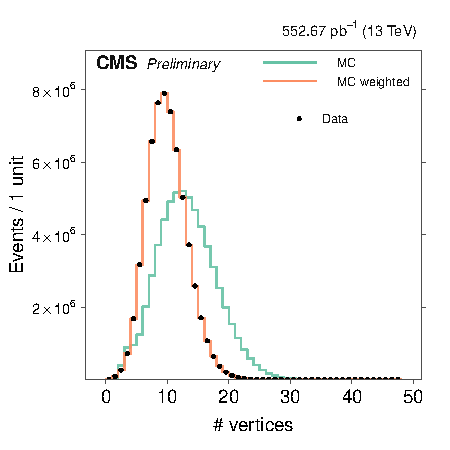
\includegraphics[scale=1.00]{figures/pileup_reweighting/f042_corr_nVert_data_mc_norm}
\caption{The distributions of the number of the reconstructed vertices
in the data, the simulated events, and the reweighted simulated events.
One is added to the the number of the reconstructed vertices.}
\label{f042_corr_nVert_data_mc_norm}
\end{figure}

The reweighting factors are derived as follows. First, we create the
distributions of the numbers of the reconstructed vertices for the data
and simulated sample. In creating these distributions, we add one to the
number of the reconstructed vertices. This is because these events do
not have the vertex for the main interaction while the events in the
signal and control regions do. Second, we smooth each distribution with
the smoothing spline. Third, we take the ratio of the two distributions,
i.e., the data over the simulated sample. The ratio is a function of the
number of reconstructed vertices. The ratio becomes reweighting factors
after normalised. The reweighting factors are normalised so as to
preserve the number of the generated events.

Figure~\ref{f042_corr_nVert_data_mc_norm} shows the distributions of the
number of the reconstructed vertices in the data, the simulated events,
and the reweighted simulated events. In the figure, one is added to the
the number of the reconstructed vertices. The figure demonstrates that
the reweighted simulated events have the distribution of the number of
the reconstructed vertices nearly identical to that in the data.


\subsection{Cross sections for SM samples}
Several MC samples of individual SM processes are binned according to a generator level quantity, such as the partonic \HT or bosonic \PT.
This analysis chooses to use samples binned in partonic \HT, for the set of MC samples (W+jets, DY+jets, QCD, $\gamma$+jets, $Z\rightarrow \nu\nu$+jets) and $\hat{P_{T}}$
for only the QCD sample.
These binned samples are provided with LO cross sections. The \kfactors required to go from LO to NNLO cross section are typically determined using corresponding
inclusive samples applied to each \HT binned sample.
Further studies can provide additional corrections to the cross sections, which can prove important to the closure test procedures described in
Section \ref{sec:closure-tests-desc}. As can be seen in Section \ref{sec:sideband_corrections}, residual cross section
corrections are measured using data in sidebands designed to enriched specific processes.

Following an inclusive selection, the distribution of the MC samples with respect to the binning variable $H_{T}^{parton}$ are shown in Fig.~\ref{fig:Lhe_Ht}, with
also the $\hat{P_{T}}$ distribution for QCD.

As stated above, the distributions shown in Fig.~\ref{fig:Lhe_Ht} follow an inclusive selection, whereby there is no requirement on each event. This direct translation
from MC allows to merge the binned generator level variable, and exhibits a smooth shape with respect to the cross sections in question.

A more in depth, data-driven investigation of the cross sections is shown in Sec.~\ref{sec:sideband_corrections}. Of which, an important point to note is that
the corrections to the cross sections, derived with the data sidebands are only relevant for data/MC comparison plots and the suite of closure tests defined in Section \ref{sec:closure-tests-desc}.

\begin{figure}[!h]
  \begin{center}
    \subfigure[$Z\rightarrow \nu\nu$ +jets] {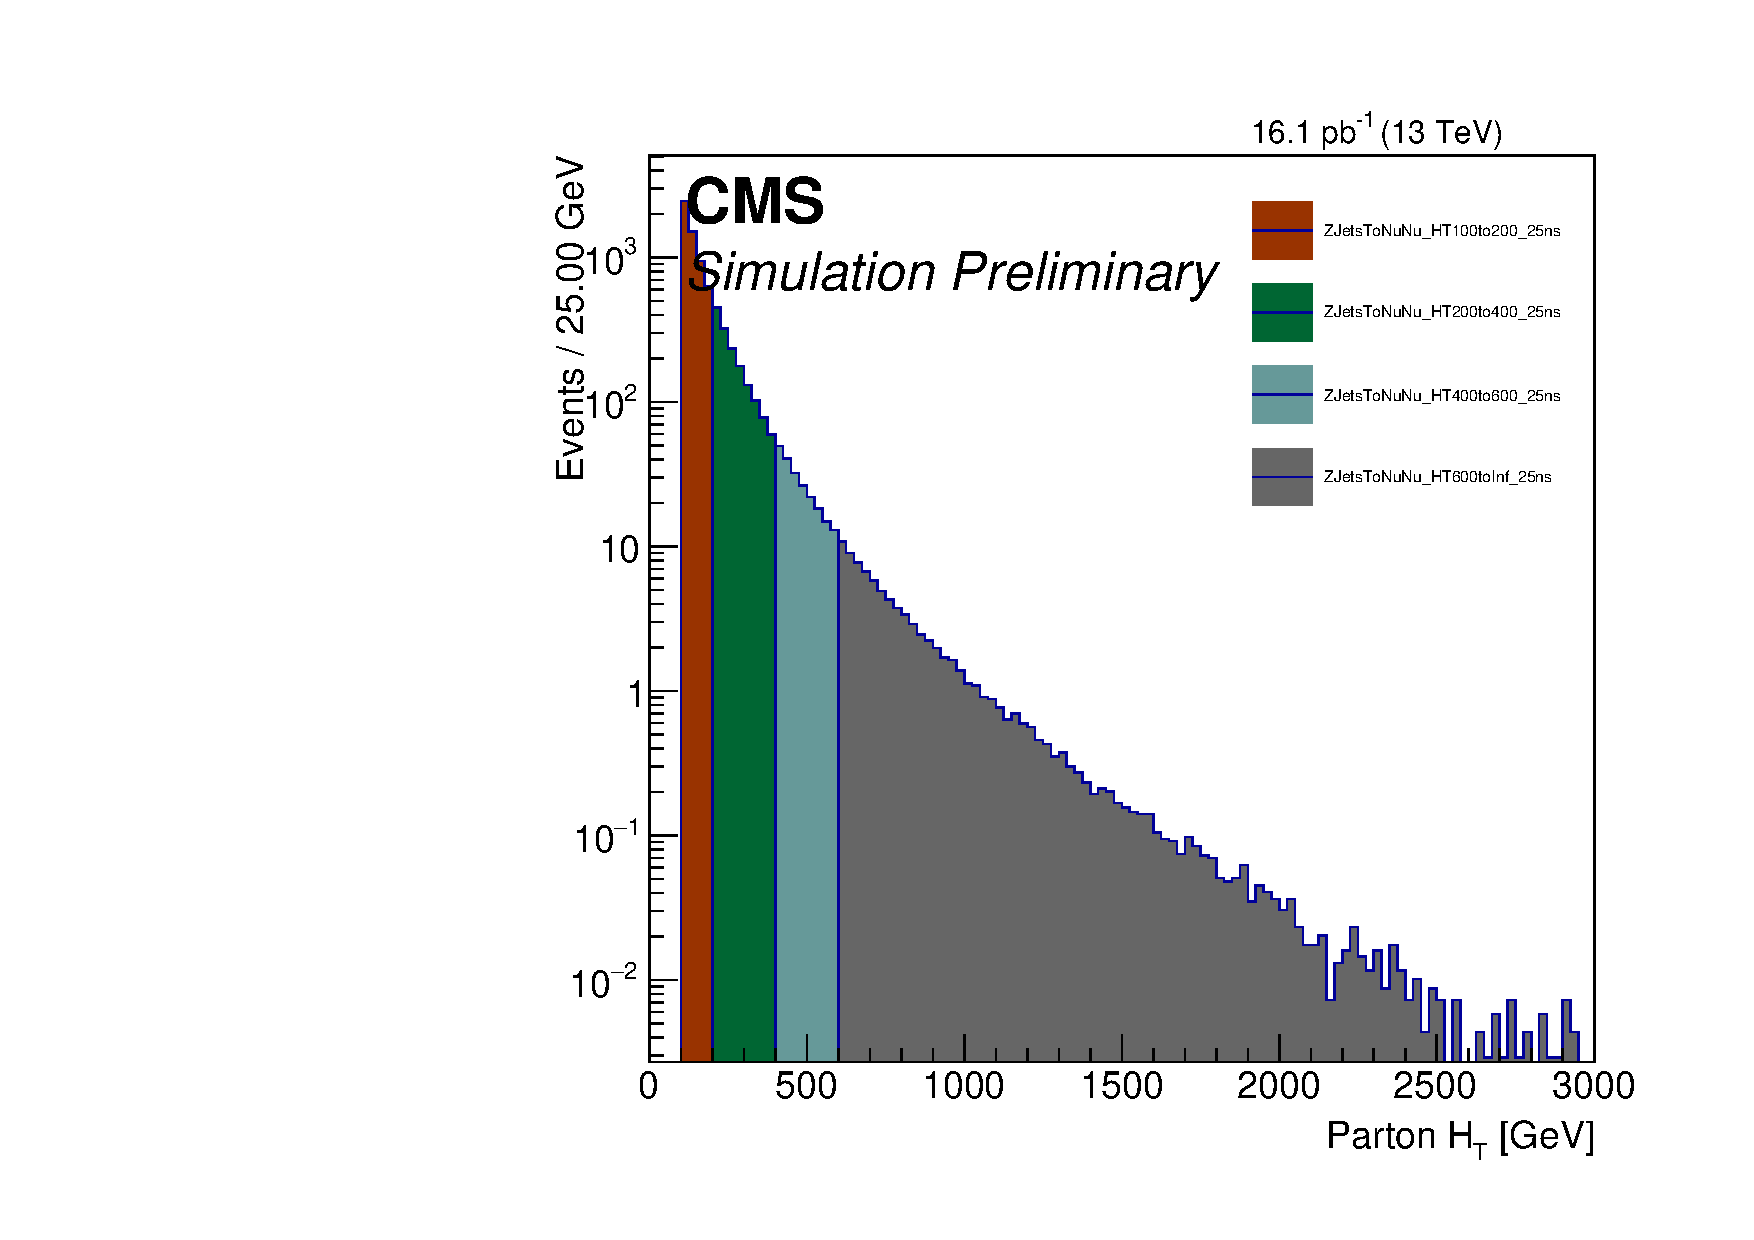
\includegraphics[width=0.45\textwidth]{figures/binnedMCsamples/Zinv.pdf}} ~~
    \subfigure[$W\rightarrow l \nu$ + jets]{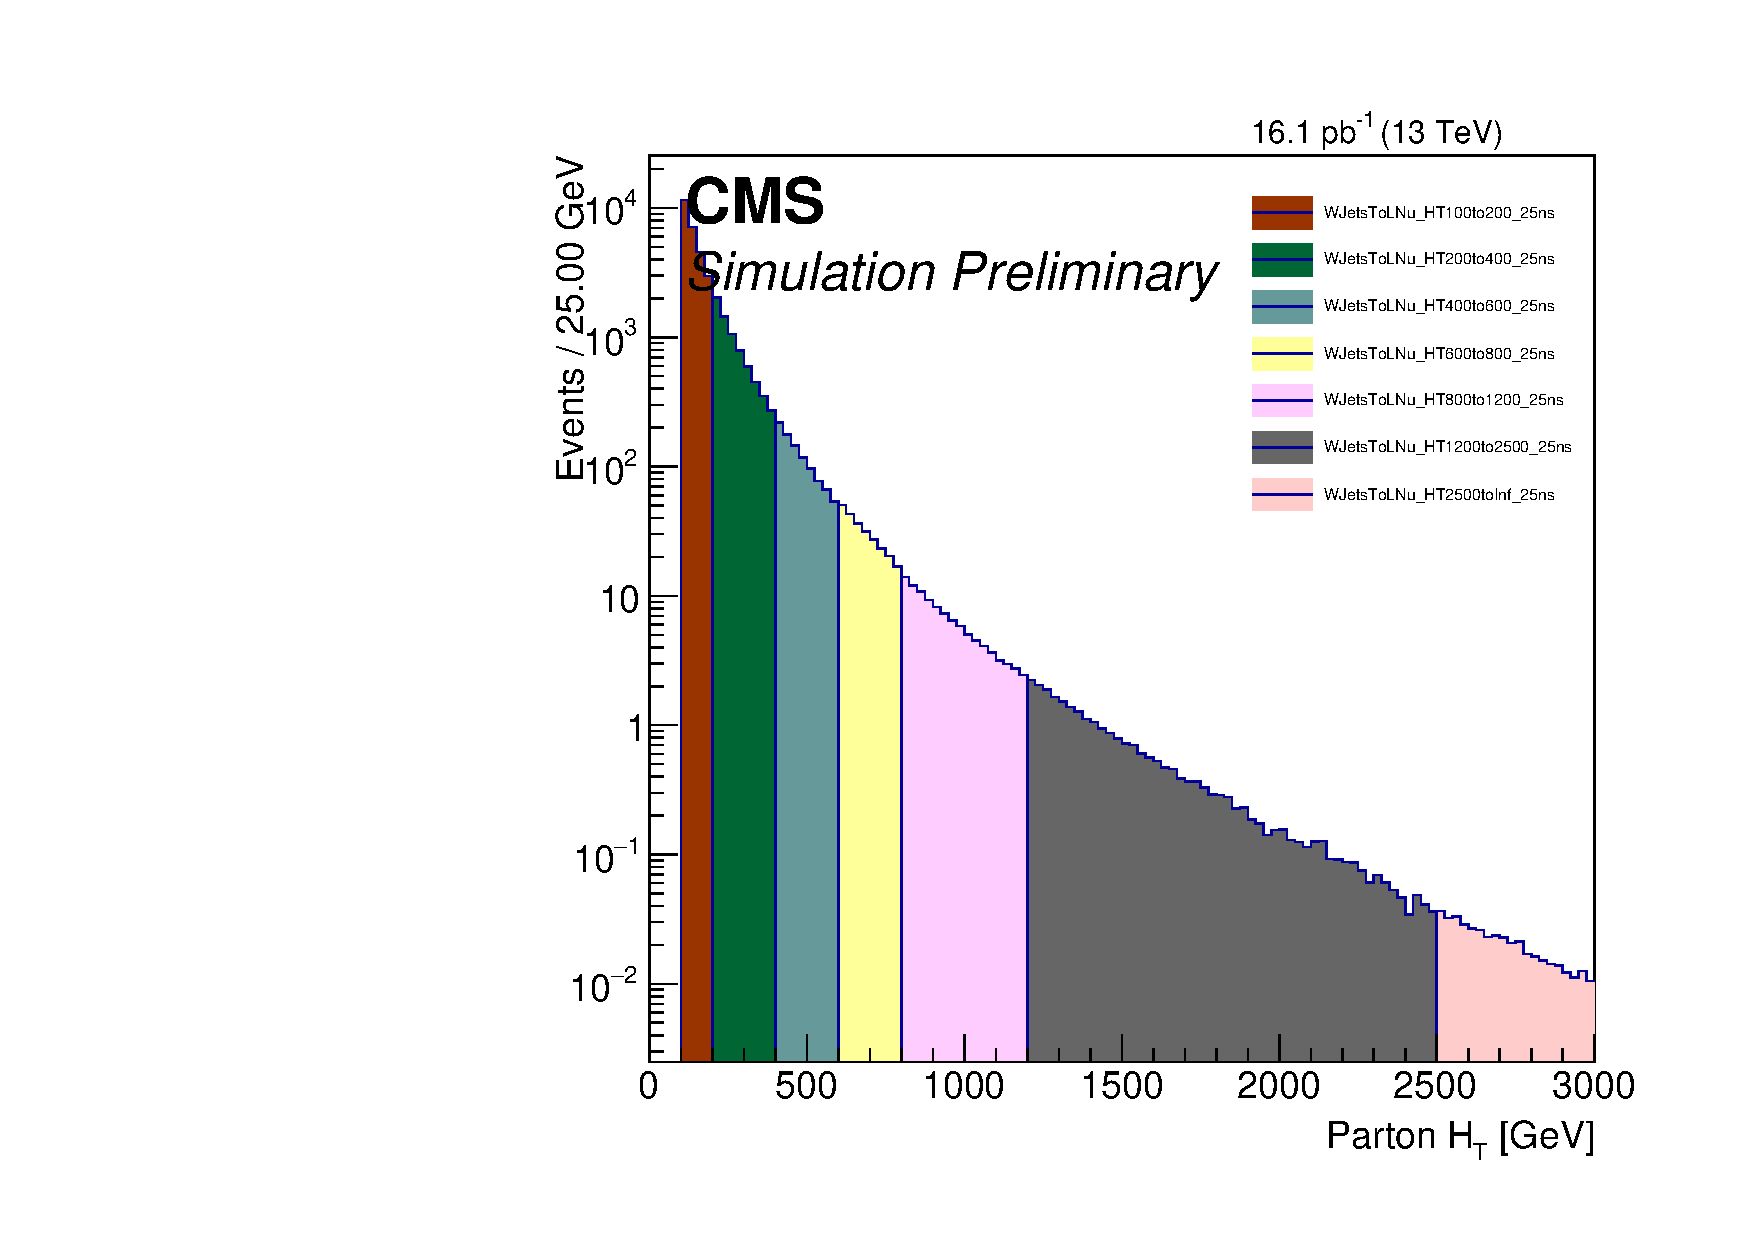
\includegraphics[width=0.45\textwidth]{figures/binnedMCsamples/WJetsToLNu_HT.pdf}} \\
    \subfigure[$DY\rightarrow ll$ + jets]{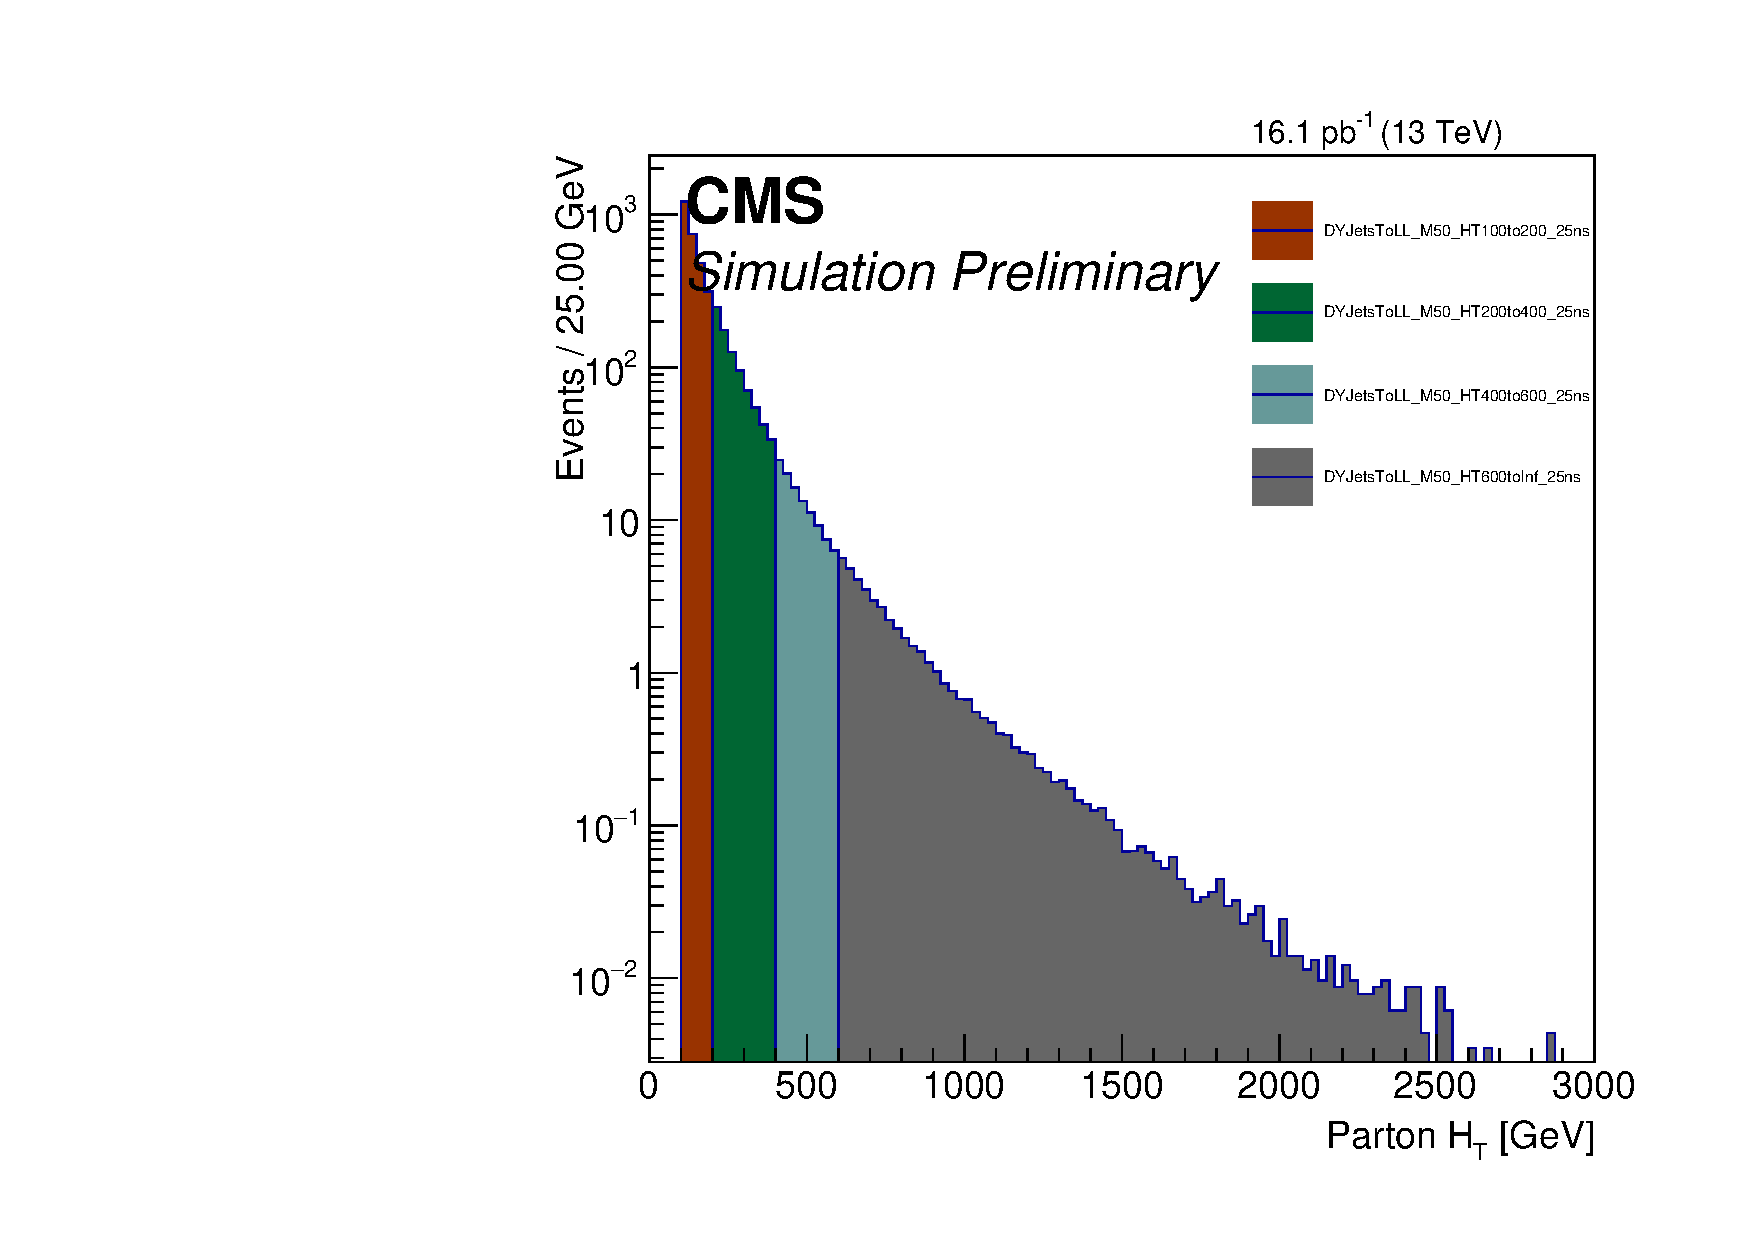
\includegraphics[width=0.45\textwidth]{figures/binnedMCsamples/DYJetsToLL_M50_HT.pdf}} ~~
    \subfigure[QCD]{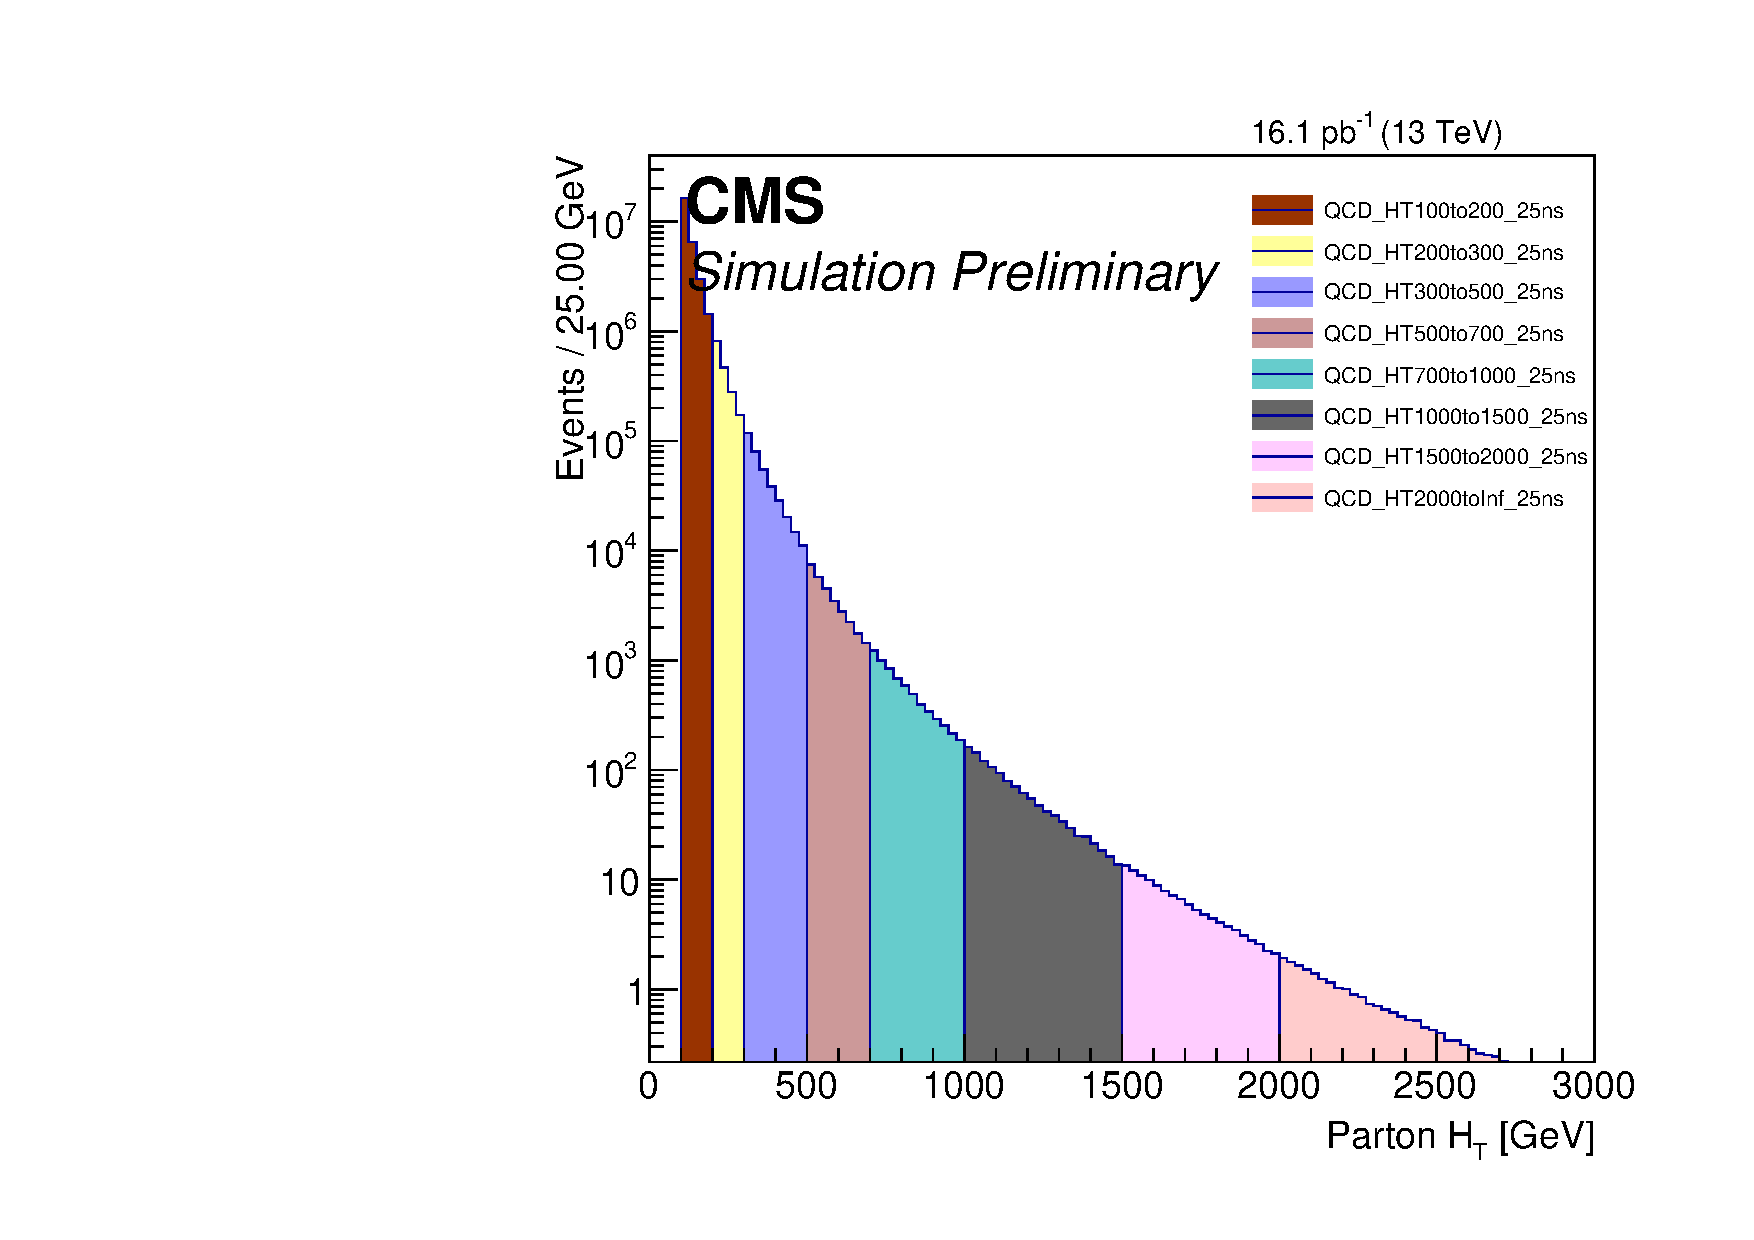
\includegraphics[width=0.45\textwidth]{figures/binnedMCsamples/QCD_HT.pdf}} \\
    \subfigure[$\gamma$+jets]{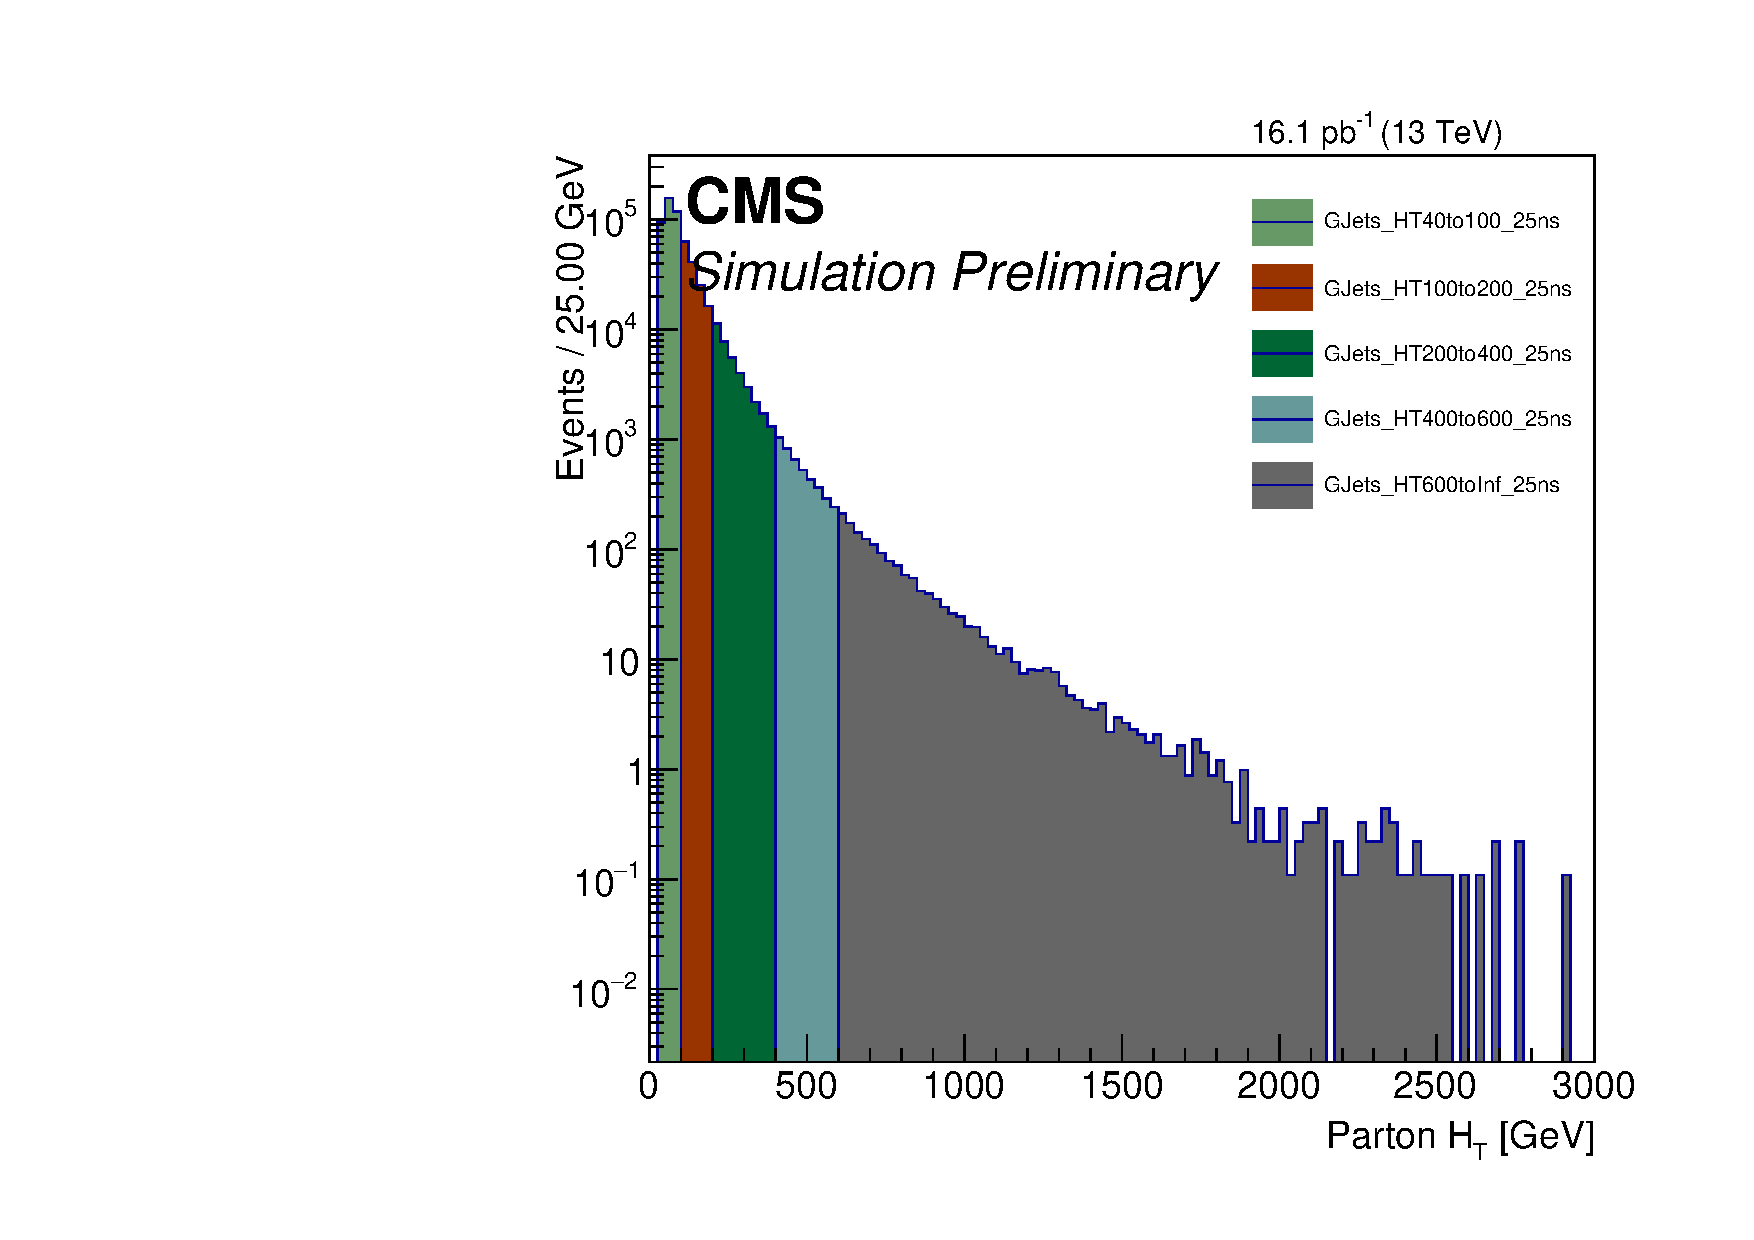
\includegraphics[width=0.45\textwidth]{figures/binnedMCsamples/GJets_HT.pdf}} ~~
    \subfigure[QCD $\hat{P_{T}}$]{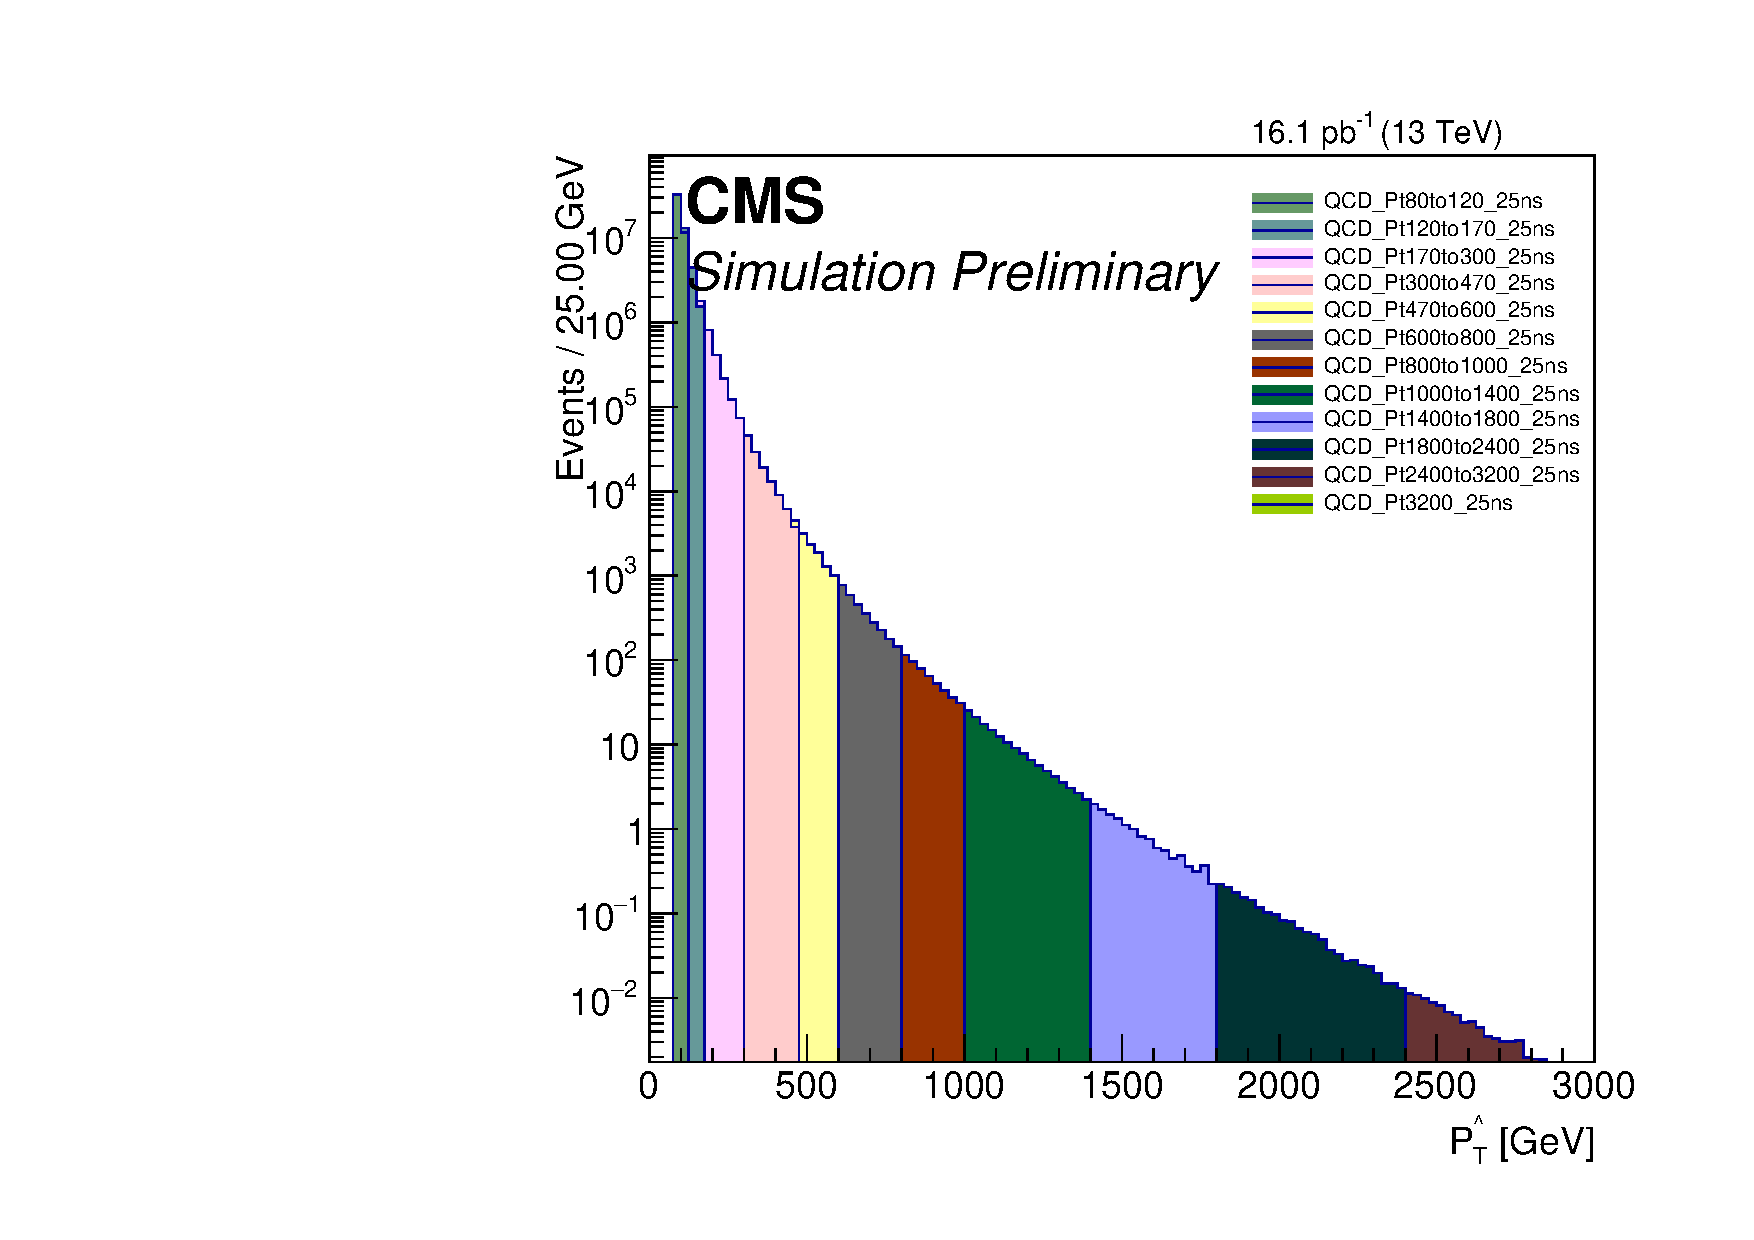
\includegraphics[width=0.45\textwidth]{figures/binnedMCsamples/QCD.pdf}}\\
    \caption{Generator-level $H_{T}^{parton}$ distributions for SM process, $Z\rightarrow \nu\nu$ + jets, W+jets, DY+jets, QCD, $\gamma$+jets, and $\hat{P_{T}}$ for QCD.}
    \label{fig:Lhe_Ht}
  \end{center}
\end{figure}

%%____________________________________________________________________________||

%%____________________________________________________________________________||
\section{Triggers}
\label{sec:triggers}


\subsection{Hadronic signal region}

In Run 2 the RA1 analysis will aim to retain the low-thresholds of Run 1 with developments to the trigger selection, maintaining sensitivity to signatures of new physics with hadronic energy as low as $\scalht = 200$ GeV. This in part is achieved by a migration to PF-based online jet reconstruction with a reduced radius parameter $\Delta R = 0.4$, which provides improvements in jet energy resolution in high-pileup conditions over calorimeter-based reconstruction and mitigates the effects of pileup contamination within the jet cone.

The hadronic signal selection is performed with $\scalht$-$\alphat$ cross triggers with a second jet threshold requirement (\verb!HLT_PFDijetXXXHTYYYAlphaTZZZ!), which suppresses QCD multijet events whilst maintaining signal acceptance.  A loose calorimeter trigger prefilter is utilised to reduce the pass-through rate prior to track-based reconstruction, ensuring the PF-based filters meet the HLT mean timing limit of $\sim$10 ms. The calorimeter prefilter utilises loose $\scalht$ and dijet $\pt$ requirements in addition to a new variable $\alphat$', defined as $\alphat$ in the limit $\Delta\scalht \rightarrow 0$, which better correlates $\alphat$ between calorimeter and PF-based reconstruction.

Each of the signal triggers uniquely seed a single offline analysis bin with the exception of the highest-$\scalht$ trigger which is utilised for analysis bins above $\scalht > 400$ GeV. Analysis bins at very high-$\scalht$ are seeded by the \verb!HLT_PFHT900! trigger with no explicit dependence on $\alphat$ or second jet threshold. A list of Run 2 triggers for the hadronic signal region in the Run 2 HLT menu are shown in Table~\ref{tab:2015_Hadronic_Signal_Triggers}. The thresholds of the triggers will remain unchanged through run conditions and are measured to give high efficiencies in all three proposed run conditions: PU40bx50, PU20bx25 and PU40bx25. The Level-1 seeds for the HLT paths are given by the disjunction of the lowest unprescaled Level-1 hadronic scalar energy and missing energy sum seeds (\verb!HTTXXX_OR_ETMYYY!) for the run scenario.

Studies are currently underway to extend the trigger strategy to increase acceptance to monojet-like signatures of compressed spectrum and DM models with the transition from a pure dijet $\pt$ requirement to a dijet average $\pt$ trigger, enabling an increase in efficiency in the selection of events exhibiting asymmetric jet topologies.


% TABLE : 2015 triggers
%----------------------------------------------------------------------
\begin{table}[h!]
\topcaption{Hadronic signal region HLT paths for the Run 2 PU40bx25 scenario, lower threshold Level-1 seeds, {\verb!HTT150 OR ETM60}, are utilised for the PU40bx50 and PU20bx50 scenarios. }
\footnotesize
\centering
\begin{tabular}{c|ccc|c} 
\hline
\hline
HLT path & L1 seed & HLT calo-prefilter                      & HLT PF-filter                          & Rate \\[0.7 ex] 
         &         & ($\scalht$, $\alphat$', $\pt^{\rm j2}$) & ($\scalht$, $\alphat$, $\pt^{\rm j2}$) & (Hz) \\[0.7 ex] 
\hline
\verb!HLT_PFDijet90HT200AlphaT0p57! & \verb!HTT175 OR ETM70! & 150, 0.540, 70 & 200, 0.570, 90 & 11.0 $\pm$ 3.0 \\
\verb!HLT_PFDijet90HT250AlphaT0p55! & \verb!HTT175 OR ETM70! & 200, 0.535, 70 & 250, 0.550, 90 & 8.5  $\pm$ 3.0 \\
\verb!HLT_PFDijet90HT300AlphaT0p53! & \verb!HTT175 OR ETM70! & 250, 0.525, 70 & 300, 0.530, 90 & 9.5  $\pm$ 3.0 \\
\verb!HLT_PFDijet90HT350AlphaT0p52! & \verb!HTT175 OR ETM70! & 300, 0.520, 70 & 350, 0.520, 90 & 10.0 $\pm$ 3.0 \\
\verb!HLT_PFDijet90HT400AlphaT0p51! & \verb!HTT175 OR ETM70! & 370, 0.510, 70 & 400, 0.510, 90 & 13.5 $\pm$ 3.5 \\
\hline
\multicolumn{4}{c|}{Exclusive rate (Hz)} & 34 $\pm$ 6 \\
\hline
\hline

\end{tabular}
\label{tab:2015_Hadronic_Signal_Triggers}
\end{table}




%Prescaled control region triggers
\subsection{Control samples}
Prescaled $\scalht$-dijet triggers, each with an exclusive rate of $\sim$1 Hz, are utilised in the selection of events for the hadronic control region. These share the same Level-1 seeds and $\scalht$ threshold of the signal triggers and are similarly each mapped to a unique offline bin. The non-hadronic control regions will be seeded by the lowest-threshold unprescaled triggers of the given run scenario, with \verb!HLT_Ele27_eta2p1_WP75_Gsf! seeding the electron control region ($e$, $ee$), \verb!HLT_IsoMu20_eta2p1! the muon control region ($\mu$, $\mu\mu$) and \verb!HLT_Photon175! the photon control region.





\subsection{Low-$\scalht$ Level-1 seeds}

Some models of new physics, such as supersymmetric compressed spectrum models, are challenging to select at the trigger level due to low-hadronic energy visible in the final state. Sensitivity to such models require low trigger thresholds which is difficult to achieve without incurring a large increase in the Level-1 trigger rate. New Level-1 seeds which enable low thresholds to be utilised by actively vetoing QCD event topologies have been studied and are shown to have higher efficiencies for such models than can be achieved with the current Level-1 menu.

The $\Delta\phi(j_{1}^{L1},j_{2}^{L1})$ seed exploits the typical dijet topologies exhibited in QCD dijet production by vetoing events where the azimuthal separation of the leading jets exceeds eight calorimeter regions, corresponding to a veto of: $\Delta\phi(j_{1}^{L1},j_{2}^{L1}) \ge 160^{\circ}$, where a jet threshold of $\pt > 32$ GeV is imposed on the second jet. This enables a much lower threshold on the $\scalht$-leg to be achieved, with a small increase in other thresholds in the menu, enabling for example the rate neutral trigger: \verb!L1_DoubleJetC32_WdPhi7_HTT125! to be utilised.

An alternate $\mht/\scalht$ 'reduced-MHT' seed exploits the correlation in missing hadronic energy and visible hadronic energy typical of decays with genuine $\met$ and the decorrelation of these quantities for QCD with fake-$\met$ by requiring a minimum $\mht/\scalht$ ratio. This again enables triggers with a significant reduction in the threshold on the $\scalht$-leg, for example with the rate neutral trigger: \verb!L1_HTT125_rHTM0p3!.

The logical disjunction of these two seeds can further improve signal efficiency whilst maintaining an effective suppression of QCD events by increasing acceptance to additional topolgies. ISR-dominated final states for instance typically have large $\mht/\scalht$ but may fail the $\Delta\phi(j_{1}^{L1},j_{2}^{L1})$ selection, where as events with high jet multiplicities typically have high $\Delta\phi(j_{1}^{L1},j_{2}^{L1})$ but may fail the $\mht/\scalht$ threshold due to the breakdown in $\mht/\scalht$ at high jet multiplicities. Combined these seeds allow even smaller thresholds to be used on the $\scalht$-leg without loss of efficiency to ISR-dominated or high jet multiplicity events, for example with the trigger:\\ \verb!L1_HTT110_rHTM0p6_rHTM0p0_WdPhi6!.


\subsubsection{Implementation and performance of low-$\scalht$ Level-1 seeds}

The new trigger seeds can be implemented in the trigger hardware by repurposing the bits currently utilised for $\mht$ and $\phi({\mht})$ trigger primitives with the new $\mht/\scalht$ and $\Delta\phi(j_{1}^{L1},j_{2}^{L1})$ primitives respectively. These changes have been discussed with trigger experts and are deemed to be relatively simple to implement in the calorimeter trigger firmware and will have little impact on the operation global trigger. The latest version of the Level-1 trigger emulator currently has the \verb!L1_DoubleJetC32_WdPhi7_HTT125!, \verb!L1_HTT125_rHTM0p3! and \\ \verb!L1_HTT110_rHTM0p6_rHTM0p0_WdPhi6! low-$\scalht$ trigger primitives implemented, enabling a wider study within the collaboration.

The performance after the full offline selection of the low-$\scalht$ Level-1 seeds was studied for a range of signal models in the lowest $\scalht$ and $\njet$ analysis bins which are predominantly populated by compressed models. Performance was measured relative to the current PU40bx25 Level-1 hadronic menu, {\verb!HTT175! \verb!OR! \verb!DoubleJetC100! \verb!OR! \verb!QuadJetC60! \verb!OR! \verb!ETM70!}, with the rate equivalent low-$\scalht$ menues defined as: Low-$\scalht$ seed {\verb!OR! \verb!HTT200! \verb!OR! \verb!DoubleJetC120! \verb!OR! \verb!QuadJetC60! \verb!OR! \verb!ETM70!}. The efficiencies of the proposed menues for $\njet = 2$ and $\njet = 3$, shown in Table~\ref{tab:LowHT_Seed_Signal_2Jet} and Table~\ref{tab:LowHT_Seed_Signal_3Jet} respectively, show significant improvements in trigger efficiency utilising the low-$\scalht$ seeds with respect to the current hadronic menu and similar performance to what could be obtained by reducing the $\met$ threshold without the additional 3 kHz Level-1 trigger rate this would incur.


% TABLE : Low-HT seed efficiencies - NJet = 2
%----------------------------------------------------------------------
\begin{table}[h!]
\topcaption{Trigger efficiency for $\njet = 2$, $200 < \scalht \le 300$ analysis bin and corresponding rate of the current Level-1 hadronic menu and proposed low-$\scalht$ trigger menues for a range of compressed signal models.} %sparticle and LSP masses represented by the first and second bracketed term respectively.}
\footnotesize
\centering
\begin{tabular}{cccccc} 
\hline
\hline
  Signal model & Hadronic menu & $\Delta\phi(j_{1}^{L1},j_{2}^{L1})$ & $\mht/\scalht$ &$\Delta\phi(j_{1}^{L1},j_{2}^{L1})$ \verb!OR! $\mht/\scalht$ & Hadronic menu \verb!OR ETM60! \\
\hline
  T2cc(250, 210)   & 0.60 & 0.86 & 0.91 & 0.94 & 0.95 \\
  T2qq(400, 400)   & 0.63 & 0.82 & 0.88 & 0.95 & 0.94 \\
  T2tt(300, 200)   & 0.53 & 0.91 & 0.95 & 0.99 & 0.96 \\
\hline
  Menu rate (kHz) & 15   & 15   & 15   & 15   & 19   \\
\hline
\hline
\end{tabular}
\label{tab:LowHT_Seed_Signal_2Jet}
\end{table}

% TABLE : Low-HT seed efficiencies - NJet = 3
%----------------------------------------------------------------------
\begin{table}[h!]
\topcaption{Trigger efficiency for $\njet = 3$, $200 < \scalht \le 300$ analysis bin and corresponding rate of the current Level-1 hadronic menu and proposed low-$\scalht$ trigger menues for a range of compressed signal models.} %sparticle and LSP masses represented by the first and second bracketed term respectively.}
\footnotesize
\centering
\begin{tabular}{cccccc} 
\hline
\hline
  Signal model & Hadronic menu & $\Delta\phi(j_{1}^{L1},j_{2}^{L1})$ & $\mht/\scalht$ &$\Delta\phi(j_{1}^{L1},j_{2}^{L1})$ \verb!OR! $\mht/\scalht$ & Hadronic menu \verb!OR ETM60! \\
\hline
  T2cc(250, 210)   & 0.45 & 0.74 & 0.74 & 0.83 & 0.94 \\
  T2qq(400, 400)   & 0.46 & 0.88 & 0.88 & 0.93 & 0.92 \\
  T2tt(300, 200)   & 0.41 & 0.76 & 0.83 & 0.84 & 0.86 \\
\hline
  Menu rate (kHz) & 15   & 15   & 15   & 15   & 19   \\
\hline
\hline
\end{tabular}
\label{tab:LowHT_Seed_Signal_3Jet}
\end{table}



%%____________________________________________________________________________||

%%____________________________________________________________________________||
\section{Physics objects}
\label{sec:objects}
The definitions of the physics objects used in this analysis follow the ongoing recommendations of the various Physics Object Groups (POGs) and PHYS14 subgroup investigations. 

\subsection{Jets}
\label{sec:jetreco}
Jets are defined as sets of particle-flow candidates clustered by the
anti-$k_{T}$ jet clustering algorithm with a distance parameter of 0.4
(PFJets). The Charged Hadron Subtraction (CHS) is applied, i.e., charged
hadrons that can be traced back to pileup vertices are not clustered.
The four-momenta of jets are initially defined as the four-vector sum of
the four-momenta of the constituent particle-flow candidates and then
scaled by the jet energy correction factors designated as L1FastJet,
L2Relative, and L3Absolute.

It should be noted that the early L1 FastJet corrections require
improvements at this stage, and as a result can impact the L2 and L3
corrections. The Tight working point Jet-Id selection criteria was
chosen for the PHYS14 investigation. Figure REF,REF and REF shows the
jet closure in simulation as a function of $p_{T}$, for the $\mu +$
jets, $\mu\mu +$ jets, and $\gamma$ + jets control sample

\subsection{b-tagged jets}
\label{sec:btags}
Jets originating from bottom quarks are identified through vertices that are displaced with respect to the primary interaction \cite{b-tagging}. The algorithm used to tag b-jets is the Combined Secondary Vertex tagger V2, using the ``Medium`` working point, which is achieved by requiring a cut of $>$ 0.814 on the algorithm discriminator variable and results in a gluon/light-quark mis-tag rate of 1.0623 $\%$ ( where ``light`` means $\it{u}$, $\it{d}$ and $\it{s}$ quarks).



\subsection{Muons}
\label{sec:muon-id}
Muons are identified according to the Tight working point definition ($\sim$ 95 $\%$ efficiency ) of the muon identifiction algorithim. A PF-based ``combined relative`` isolation is determined within a cone size of $\Delta R < 0.4 $, and ``$\rho$``corrections are applied to remove the effects of pileup. Isolated muons are required to have minimal energy from neutral and charged PF candidates. A cone of $\Delta R$ = 0.4 is formed around the candidate lepton trajectory, and the transverse momenta is summed over PF neutral and charged candidates, excluding that of the lepton itself. The relative combined isolation $I^{rel}_{comb}$ is then defined as the ratio of this scalar sum to the transverse momentum of the lepton candidate. 
Figures REF show the relative combined isolation $I^{rel}_{comb}$ for $\mu +$ jets and $\mu\mu +$ jets control sample. The distributions have been weighted according to the cross-section of the respective samples in each region, and an integrated luminosity of 1 fb$^{-1}$ at $\sqrt{s}$ = 13 TeV. Isolated muons promptly produced in the decays of W and Z bosons dominate the region $I^{rel}_{comb}$ $<$ 0.12.
In the case of high jet multiplicity events, an increase in energy resulting in boosted events can result in complicated topologies for leptons and jets. For example high $p_{T}$ top quarks decaying leptonically, the main issue is the small angular separation between that of the lepton and the b-jet. Classical lepton isolation techniques will reject the boosted leptonic top quarks. A solution to this is to reduce the cone size around the lepton in function of $p_{T}$. This technique known as Mini Isolation is currently being investigated as a potential candidate for increasing the prompt lepton efficiency in boosted topologies.  

Muons are used as a veto as part of the hadronic signal region definition, as described in Section REF, and as part of the $\mu +$ jets and $\mu\mu +$ jets control sample selections as described in Section REF.


\subsection{Photons}
\label{sec:photon-id}
Photons are identified according to the Tight working point defintion ($\sim$ 70 $\%$ efficiency) of the simple cut-based photon identification algorithm \cite{photon-id}. PF-based isolation is determined within a cone size $\Delta R$ $<$ 0.3 and $\rho$ x $A_{eff}$ corrections are applied to remove the effects of pileup \cite{pf-photon}. Table REF summarises the identification and isolation requirements for PHYS14 samples. 
This object is used as a veto as part of the hadronic signal region definiton, as described in Section REF, and as part of the $\gamma$ + jets control sample described in Section 7.4.4.

\begin{table}[ht!]
  \caption{Photon identification (Tight working point).\label{tab:photon-id-gamma}}
  \centering
  \footnotesize
  \begin{tabular}{ ccc }
    \hline
    \hline
    Categories                    & Barrel                             & EndCap                             \\
    \hline
    Conversion safe electron veto & Yes                                & Yes                                \\
    Single Tower H/E              & 0.012                              & 0.011                               \\
    $\sigma_{i\eta i\eta}$        & 0.098                              & 0.0264                               \\
    PF charged hadron isolation   & 1.91                               & 1.26                               \\
    PF neutral hadron isolation   & 2.55 + 0.0023 $\times$ $\pt^{\gamma}$  & 2.71 + 0.0116 $\times$ $\pt^{\gamma}$  \\
    PF photon isolation           & 1.29 + 0.0004 $\times$ $\pt^{\gamma}$ & 1.91 + 0.0037 $\times$ $\pt^{\gamma}$ \\
    \hline
    \hline
  \end{tabular}
  \end{table}


\subsection{Electrons}
\label{sec:electron-id}
Electrons are identified according to the Loose working point definition ( $\sim$ 90 $\%$ efficiency ) of the cut-based identification \cite{electron-id}. PF-based isolation \cite{pf-photon} is determined within a cone size of $\Delta R$ $<$ 0.3 and $\Delta \beta$ corrections are applied to remove the effects of pileup. Table REF summarises the identification and isolation requirements derived using the PHYS14 samples. 	

\begin{table}[h!]
  \caption{Electron identification (Loose working point).\label{tab:ele-id}}
  \centering
  \footnotesize
  \begin{tabular}{ lcc }
    \hline
    \hline
    Categories                                               & Barrel    & EndCap    \\
    \hline
    $\Delta \eta_{In}$                                       & 0.010557  & 0.010654  \\
    $\Delta \phi_{In}$                                       & 0.012442  & 0.145129  \\
    $\sigma_{i\eta i\eta}$                                   & 0.072624  & 0.032602  \\
    H/E                                                      & 0.121476  & 0.131862  \\
    d0 (vtx)                                                 & 0.022664  & 0.097358  \\
    dZ (vtx)                                                 & 0.173670  & 0.198444  \\
    $\lvert(1/E_{\textrm{ECAL}} - 1/p_{\textrm{trk}})\rvert$ & 0.221803  & 0.142283  \\
    PF relative isolation                                    & 0.120026  & 0.162914  \\
    Missing hits                                             & 1         & 1         \\
    \hline
    \hline
  \end{tabular}
  \end{table}


\subsection{Single Isolated Tracks}
\label{sec:SIT}

A single isolated track (SIT) can be used to identify W bosons through their leptonic decays: W $\rightarrow$ $\mu \nu$, W $\rightarrow$ $e\nu$, and W $\rightarrow$ $\tau$($\rightarrow l$) $\nu$. Single prong decays of the tau lepton can be identified: W $\rightarrow$ $\tau$ ($\rightarrow$ h$^{\pm}$ + n$\pi^{0}$) $\nu$. A single isolated track comprises a charged PF candidate that satisfies the requirements listed in Table REF. The relative track isolation is determined from the vectorial sum of neighbouring charged PF candidates within a cone $\Delta R$ $<$ 0.3 and satisfying $\Delta$z(candidate, PV) $<$ 0.05cm around the candidate isolated track.
This object can be used to efficiently suppress the ``lost lepton`` background from W and t$\bar{t}$, as described in Section 7.1. 


\subsection{Missing transverse momenum}
Missing transverse momentum is defined as the negative of the vector sum
of the transverse momentum of all particle-flow candidates in the event.
The Type-I MET correction is applied, i.e., the transverse momentum of
the particle-flow candidates clustered as jets are replaced with the
transverse momentum of the jets that are scaled by the jet energy
correction factors.

The missing transverse momentum is only used in the following two cases:
to define the transverse mass, $M_{T}$, which is in turn used as part of
the selection criteria that define the $\mu +$ jets control sample,
described in REF, and to define a cleaning filter applied after the
$\alpha_{T}$ requirement, as described in REF.



%%____________________________________________________________________________||

%____________________________________________________________________________||
\section{Event selection for signal and control regions}
\label{sec:selection}

This section first outlines the set of ``pre-selection'' requirements
that are common to all signal and control regions, before defining the
selection criteria that are specific to each region.

%%____________________________________________________________________________||
\subsection{Pre-selection}
\label{sec:preSelection}

{\bf Removing instrumental sources of ``fake'' \met.} 

A number of beam- and detector-related effects can induce significant
\met. Examples include beam halo, reconstruction failures, spurious
detector noise, or event misreconstruction due to detector
inefficiencies. These events, with large, non-physical values of \met,
are rejected with high efficiency by applying a range of dedicated
vetoes. All ``MET filters'' recommended by the JetMET POG and SUSY PAG
will be applied by default in this analysis, listed in Table ~\ref{tab:pre-selections}.

{\bf Jet requirements.} 

Jets considered in the analysis are required to satisfy $\PT>40\gev$
and $|\eta|<3.0$. Events containing jets in the forward region that
satisfy the requirements $\PT>40\gev$ and $|\eta|>3.0$ are rejected in
order to control background contributions from SM processes, without
introducing a significant reduction in signal acceptance. The jets
that are selected are used in the calculation of all jet-based
event-level variables, such as \HT, \mht, and \alphat.

Raised $\PT$ thresholds and tighter $\eta$ requirements on the lead jets 
are also required. The lead jet is required to satisfy $\PT > 100\gev$
and $|\eta|<2.5$. This helps to ensure high trigger efficiencies,
but also helps to improve the S/B for a wide
range of models with respect to SM processes, such as V + jets
production. Events are then classified based on the
second leading jet. In the case that a second leading jet satisfies $\PT > 100\gev$ 
events are assigned to a ``symmetric'' \njet category. If the second
jet satisfies $40 < \PT < 100\gev$ events are assigned to an
``asymmetric'' \njet category. Finally, if there is no second leading
jet with $\PT>40\gev$, events are assigned to the ``mono-jet''
category. The asymmetric and mono-jet categories have been added to
the analysis to help improve acceptance to a range of DM models and compressed
SUSY.

{\bf Event categorisation according to \njet and \nb.} 

Events in the hadronic signal and all control regions (described
below) are categorised identically and according to the number of jets
(\njet) reconstructed in each event and the number of jets identified
as originating from bottom quarks (\nb) in each event. As a baseline,
the resulting sub-samples comprise events containing exactly one, two,
three, four, or at least five jets. These are further split into
``monojet'' (only in the $\njet=1$ case),
``symmetric'' or ``asymmetric'' \njet categories according to the
second leading jet \Pt, as defined above.

Events are also categorised according to the the number of b-tagged
jets (``b-jets''). As a baseline, the sub-samples are defined by
requiring exactly zero, one, two, or at least three b-tagged jets. By
construction, $\nb \leq \njet$. Events containing three or more b-tags
typically implies either an additional source of b-jets beyond those
from the \ttbar process (\eg via gluon splitting) or at least one
mistag of a jet from a light-flavoured parton. The number of b-tagged
jets is currently taken directly from simulation.

In the near future, the ``b-tag formula method'' (described below and
detailed in Ref.~\cite{Chatrchyan:2013lya}) will again be employed to
improve the statistical precision of predictions involving events
containing high multiplicities of b-tagged jets, which will allow for
the addition of further categories that contain at least four b-tagged
jets. In order to maximise sensitivity to potential new physics
signatures in final states with a high b-quark content, a method that
improves the statistical power of the predictions from simulation,
particularly for $n_\cPqb \ge 2$, is employed~\cite{Chatrchyan:2013lya}. The
distribution of $n_\cPqb$ is estimated from generator-level
information contained in the simulation, namely the number of
reconstruction-level jets matched to underlying bottom quarks
($n_\cPqb^\text{gen}$), charm quarks ($n_\cPqc^\text{gen}$), and
light-flavoured partons ($n_\cPq^\text{gen}$) per event. All relevant
combinations of $n_\cPqb^{\rm gen}$, $n_\cPqc^{\rm gen}$, and
$n_{\cPq}^{\rm gen}$ are considered, and event counts are recorded
according to the categorisation of events in terms of \njet and
\scalht. The efficiency $\epsilon$ with which b-quark jets are
identified and the mistag probabilities $f_\cPqc$ and $f_\cPq$ are
also determined from simulation per event category, with each quantity
averaged over jet \pt and $\eta$. Corrections are applied on a
jet-by-jet basis to $\epsilon$, $f_\cPqc$, and $f_\cPq$ in order to
match the corresponding measurements from
data~\cite{Chatrchyan:2012jua}. This information is sufficient to
predict $n_\cPqb$ and thus also determine the event yield from
simulation for a given event category. The event yields for a given
b-quark jet multiplicity can be predicted with a higher statistical
precision than obtained directly from simulation, particularly for
events with high counts of b-quark jets.

{\bf \HT requirements and binning.} 

Events are required to have significant hadronic activity by requiring
$\scalht > 200\GeV$. Despite an increase in both multijet production
cross sections and pileup in Run~2, the lowest \HT threshold will be
kept at the same value of the Run~1 analysis~\cite{Chatrchyan:2013lya}
in order to maintain acceptance to DM models or compressed
SUSY. Events in all samples are binned identically, according to the
\HT variable. The choice of binning in \HT is driven primarily by the
trigger strategy employed by the analysis, as described in
Section~\ref{sec:triggers}, and can be summarised as follows: 50\gev
bins in the range $200 < \HT < 400\gev$, 100\gev bins in the range
$400 < \HT < 600\gev$, a 200\gev bin $600<\HT<800\gev$ and a final 
inclusive bin $\HT > 800\gev$.

The lower threshold of the last (inclusive) \HT bin is not forced to
$800\gev$, it is instead determined
independently for each (\njet,\nb) event category and is chosen to
always align with one of the ``default'' boundaries defined above. The
metric for choosing the final bin threshold is based on the number of
events in the corresponding event category and \HT bin of the data
control samples. This ensures that all bins in the data control
samples are sufficiently populated to ensure a statistically
significant prediction in each of the corresponding signal region
bins. Currently, this is achieved by requiring sufficient events
($\sim 10$) to yield a statistical uncertainty on the total background
prediction of $\lesssim30\%$. Events from high \HT bins are combined
into a single inclusive bin that satisfies this metric. This metric
also ensures that there are sufficient events in the control samples
to probe for potential systematic effects with closure tests between
simulation and data, as described in Sec.~\ref{sec:systematics}.

\begin{table}[h!]
  \topcaption{Summary of the pre-selection criteria for 3\fbinv and 10\fbinv.}
  \label{tab:pre-selections}
  \centering
  \footnotesize
  \begin{tabular}{ ll }
    \hline
    \hline
    Selection                     & Requirement                                                                          \\
    \hline
    ``MET filters''               & Primary Vertex, CSC Beam Halo, HBHE Noise and Isolation, ECAL Endcap SC Noise        \\
    Jet acceptance                & $\PT > 40\gev$, $|\eta| < 3$                                                         \\
%    \njet                         & $\geq2$                                                                \\
    Lead jet acceptance           & $\PT > 100\gev$, $|\eta| <    2.5$                                     \\
    Second jet acceptance         & $\PT > 100\gev$ \texttt{OR} $40 < \PT < 100\gev$                       \\
    Loosest \HT requirement       & $\HT > 200\gev$                                                        \\
    Baseline \HT binning          & 200--250, 250--300, 300--350, 350--400, 400--500, 500--600, 600--800, $>$800\gev \\
    Baseline \njet multiplicities & 1 (mono-jet), 2, 3, 4, $\geq$5 (both symmetric and asymmetric)                       \\
    Baseline \nb multiplicities   & 0, 1, 2, $\geq3$ ($\nb \leq \njet$)                                    \\
    \hline
    \hline
  \end{tabular}
\end{table}

{\bf Summary of pre-selection requirements for 3\fbinv and 10\fbinv.} 

Table~\ref{tab:pre-selections} summarises the pre-selection
requirements and default categorisation and binning scheme. The
threshold of the final \HT bin per (\njet,\nb) category is summarised
in Table~\ref{tab:binning-3fb}. An identical scheme is used for the
signal region and all control regions. No extrapolation is performed
in the variables \njet, \nb, and \HT in this analysis. For each of the
signal and control regions, thirty event categories are considered,
each with up to seven bins in \HT, assuming an integrated luminosity
of 3\fbinv. The same binning scheme is currently also used for the
sensitivity projections with 10\fbinv. However, this scheme will
evolve with integrated luminosity as discussed below.

\begin{table}[h!]
  \caption{Threshold (GeV) of the final \HT bin as a function of event
    category (\njet,\nb), which is always aligned with respect
    to one of the baseline boundaries (motivated primarily by the trigger) of
    200, 250, 300, 350, 400, 600, 800\gev. This is the projected choice for 3\fbinv.}
  \label{tab:binning-3fb}
  \centering
  \footnotesize
  \begin{tabular}{ l|ccc|cccc|cccc|cccc }
    \hline
    \hline
    \njet      & \multicolumn{3}{c}{2} & \multicolumn{4}{c}{3} & \multicolumn{4}{c}{4} & \multicolumn{4}{c}{$\geq5$}                                                   \\ 
    \nb        & 0                     & 1                     & 2                     & 0   & 1   & 2   & 3   & 0   & 1   & 2   & $\geq3$ & 0   & 1   & 2   & $\geq3$ \\
    \hline
    Symmetric  & 800                   & 800                   & 600                   & 800 & 800 & 800 & 400 & 800 & 800 & 800 & 600     & 800 & 800 & 800 & 800     \\
    Asymmetric & 800                   & 600                   & 400                   & 800 & 600 & 400 & 300 & 600 & 600 & 600 & 400     & 600 & 600 & 600 & 400     \\
    \hline
    \hline
  \end{tabular}
\end{table}

{\bf Evolution of event categorisation and \HT binning versus integrated luminosity.} 

The choice of how events are categorised according to the number of
\njet and \nb and binned in \HT will evolve as a function of
integrated luminosity. Additional categories with higher jet
multiplicities maybe added for data samples corresponding to higher
integrated luminosities (\eg $\sim$10\fbinv). Additional categories
with higher b-tag multiplicities will also be considered once the
b-tag ``formula method'' (described above and detailed in
Ref.~\cite{Chatrchyan:2013lya}) has been commissioned with data. This
will allow for categories defined by the requirement of at least four
b-tagged jets. Additional bins at high \HT will also be considered for
higher integrated luminosity scenarios. 

\subsection{Lepton and photon vetoes \label{sec:vetoes}}

To select a sample of events in the hadronic final state and to
suppress SM processes with genuine \met from neutrinos, events
containing an isolated electron with $\pt > 10\GeV$ and $|\eta| < 2.5$
or an isolated muon with $\pt > 10\GeV$ and $|\eta| < 2.5$ are
vetoed. Further, to reduce the ``lost leptons'' backgrounds from \wj
and \ttbar, events containing single isolated tracks with $\pt >
10\GeV$ and $|\eta| < 2.5$, as defined in Section~\ref{sec:objects},
are vetoed as part of the signal region selection criteria. In the
case of the single and di-lepton control samples, a further
requirement is made such that events are not vetoed due to the
presence of a track from the well identified leptons, by requiring
$\Delta R(\textrm{track},\textrm{lepton}) > 0.02$.

Finally, to select a pure multijet topology and to allow for a
disjoint control region, events are vetoed in which an isolated photon
with $\pt > 25\GeV$ and $|\eta| < 2.5$ is identified.

\subsection{The hadronic signal region}
\label{sec:had-signal}

The lepton and photon vetoes are applied to select hadronic final
states. All pre-selection criteria are also applied. Following these
selections, the multijet background from QCD is still several orders
of magnitude larger than the typical signal expected from SUSY.

{\bf \HT-dependent \alphat requirements.}

Background events from multijet production populate the region
$\alphat \lesssim 0.5$ and therefore can be rejected with very high
efficiency by requiring an appropriate cut on \alphat. In the Run~1
analyses, a minimum requirement of $\alphat > 0.55$ was imposed, with
a raised threshold (as high as 0.65) used at low \HT to control
against a potential increase in contamination from multijet production
due to worsening resolution and jet \PT threshold effects.  (The
latter effect refers to ``fake'' \mht arising from the rare occurrence
of multiple soft jets below threshold that are relatively collinear.)
The minimum threshold of 0.55 was motivated primarily by the control
of the multijet background and considered conservative for mid to high
regions in \HT, while maintaining good signal acceptance. However,
improving jet resolutions and a reduced jet threshold effect relative
to an increasing \HT scale means that looser \alphat thresholds can be
used at higher values of \HT.

A useful approximate conversion between \alphat and \mht can be
obtained by calculating \alphat while forcing $\dht = 0\gev$, as
described by Eq.~\ref{eq:alphat3}. Hence, using this metric, the
dependence of the \alphat requirement as a function of the \HT bin can
be determined such that the effective requirement on \mht is
comparable, \ie roughly constant, across all \HT bins. The values
typically fall in the range $\sim110 < \mht < \sim160\gev$. This
approximate levelling of the ``effective'' \mht threshold implies
increasingly tighter requirements against instrumental effects versus
\HT, while maximising signal
acceptance. Table~\ref{tab:alphat-thresholds} summarises the expected
\alphat thresholds and corresponding ``effective'' \mht thresholds for
each \HT bin. The \alphat threshold is dependent only on \HT and not
on \njet nor \nb that are used to define the event categories.

\begin{table}[h!]
  \caption{\alphat and corresponding ``effective'' \mht (GeV) thresholds versus
    lower bound of \scalht bin. For all \HT bins satisfying $\HT > 800
    \gev$, a direct requirement of $\mht > 130\gev$ is imposed rather
    than a requirement on \alphat. No \alphat requirement is imposed in the
    monojet bins.}
  \label{tab:alphat-thresholds}
  \centering
  \footnotesize
  \begin{tabular}{ lcccccccc }
    \hline
    \hline
    \scalht            & 200       & 250       & 300       & 350       & 400       & 500       & 600       \\
    \hline                                                                                     
    \alphat threshold  & 0.65      & 0.60      & 0.55      & 0.53      & 0.52      & 0.52      & 0.52      \\
    ``Effective'' \mht & $\sim$128 & $\sim$138 & $\sim$125 & $\sim$123 & $\sim$110 & $\sim$138 & $\sim$162 \\
    \hline
    \hline
  \end{tabular}
\end{table}

For Run~2, all signal region bins satisfying $\HT > 800\gev$ will be
seeded by the single-object \texttt{HLT\_HT800} trigger, which is
expected to be unprescaled. For these high \HT bins, no \alphat
threshold is required, which removes the inefficiencies of this
variable for high jet multiplicity events. Instead, the following
requirements are imposed to control the multijet background: $\mht >
130\gev$ and $\bdphi > 0.3$ (described below).

{\bf \bdphi requirement.} 

Further, an additional powerful variable \bdphi is used to suppress
multijet contamination due to both instrumental effects and
semi-leptonic heavy-flavour decays with genuine \met in the final
state. The variable is determined as follows. The jet-based estimate
of the missing transverse energy, ${\mhtvec}$, is recomputed while
ignoring one of the reconstructed jets (the ``test'' jet). The
difference in the azimuthal angle between the recomputed $\mhtvec$
and the ``test'' jet is then determined. This process is repeated for
each jet in the event and the minimum of all the azimuthal
differences, \bdphi, is determined. For monojet events, the calculation is 
performed using all jets with $\Pt > 20\gev$. The ``test'' jet whose subtraction
from the calculation $\mhtvec$ yields this minimum value, is
identified as the jet that is most likely to have given rise to the
missing transverse energy in the event. Events with significant \mht
due to instrumental effects or heavy flavour decays populate the
region $\bdphi \approx 0$ and so candidate signal event are accepted
only if they satisfy $\bdphi > 0.3$. The use of the \bdphi and \alphat
variables provide an extremely powerful rejection factor against
contamination from multijet events and allow to maintain low jet \PT,
\HT, and \mht thresholds, which in turn maximises signal acceptance
for a large range of DM and SUSY models with final states
characterised by the presence of significant \met.

{\bf $\mht/\met$ cleaning filter.} 

To protect against multiple jets failing the $\Et$ threshold, the jet-based
estimate of the missing transverse energy, \mht, is compared to the
missing transverse energy variable, $\met$, and events with $R_{\rm
  miss}=\mht/\met > 1.25$ are rejected.
  
{\bf Detector dead cell control.}

Masked regions in the ECAL (which amount to about 1\% of the ECAL channel count)
or HCAL, or by missing instrumentation in the barrel-endcap gap, could cause 
severe energy losses. A data-driven method is developed to identify dead cells. The 
procedure is as follows. For each jet in the inclusive jet collection with
$\PT > 20 \gev$ in data, the azimuthal angle ($\Delta\phi_{jet}$) between the jet and the 
recomputed ${\mhtvec}$ is determined, same as the procedure to compute the \bdphi 
variable. A $\eta$ $\phi$ map is made with each jet which gives $\Delta\phi_{jet} < 0.3$.
Finally, a $\eta$ $\phi$ map is also made with all jets in the inclusive jet collection and
a 2D ratio map is obtained with the numerator being the former and the denumerator being 
the later. Jets pointing to dead cells are likely to give $\Delta\phi_{jet} < 0.3$, so the
location of dead cells in $\eta$ and $\phi$ will have a higher value in the 2D ratio map. 
Figure~\ref{fig:2dRatioMap} is the 2D ratio map made with unblinded signal region with luminosity of 
149.49~$\text{pb}^{-1}$.

\begin{figure}[h!]
    \begin{center}
        {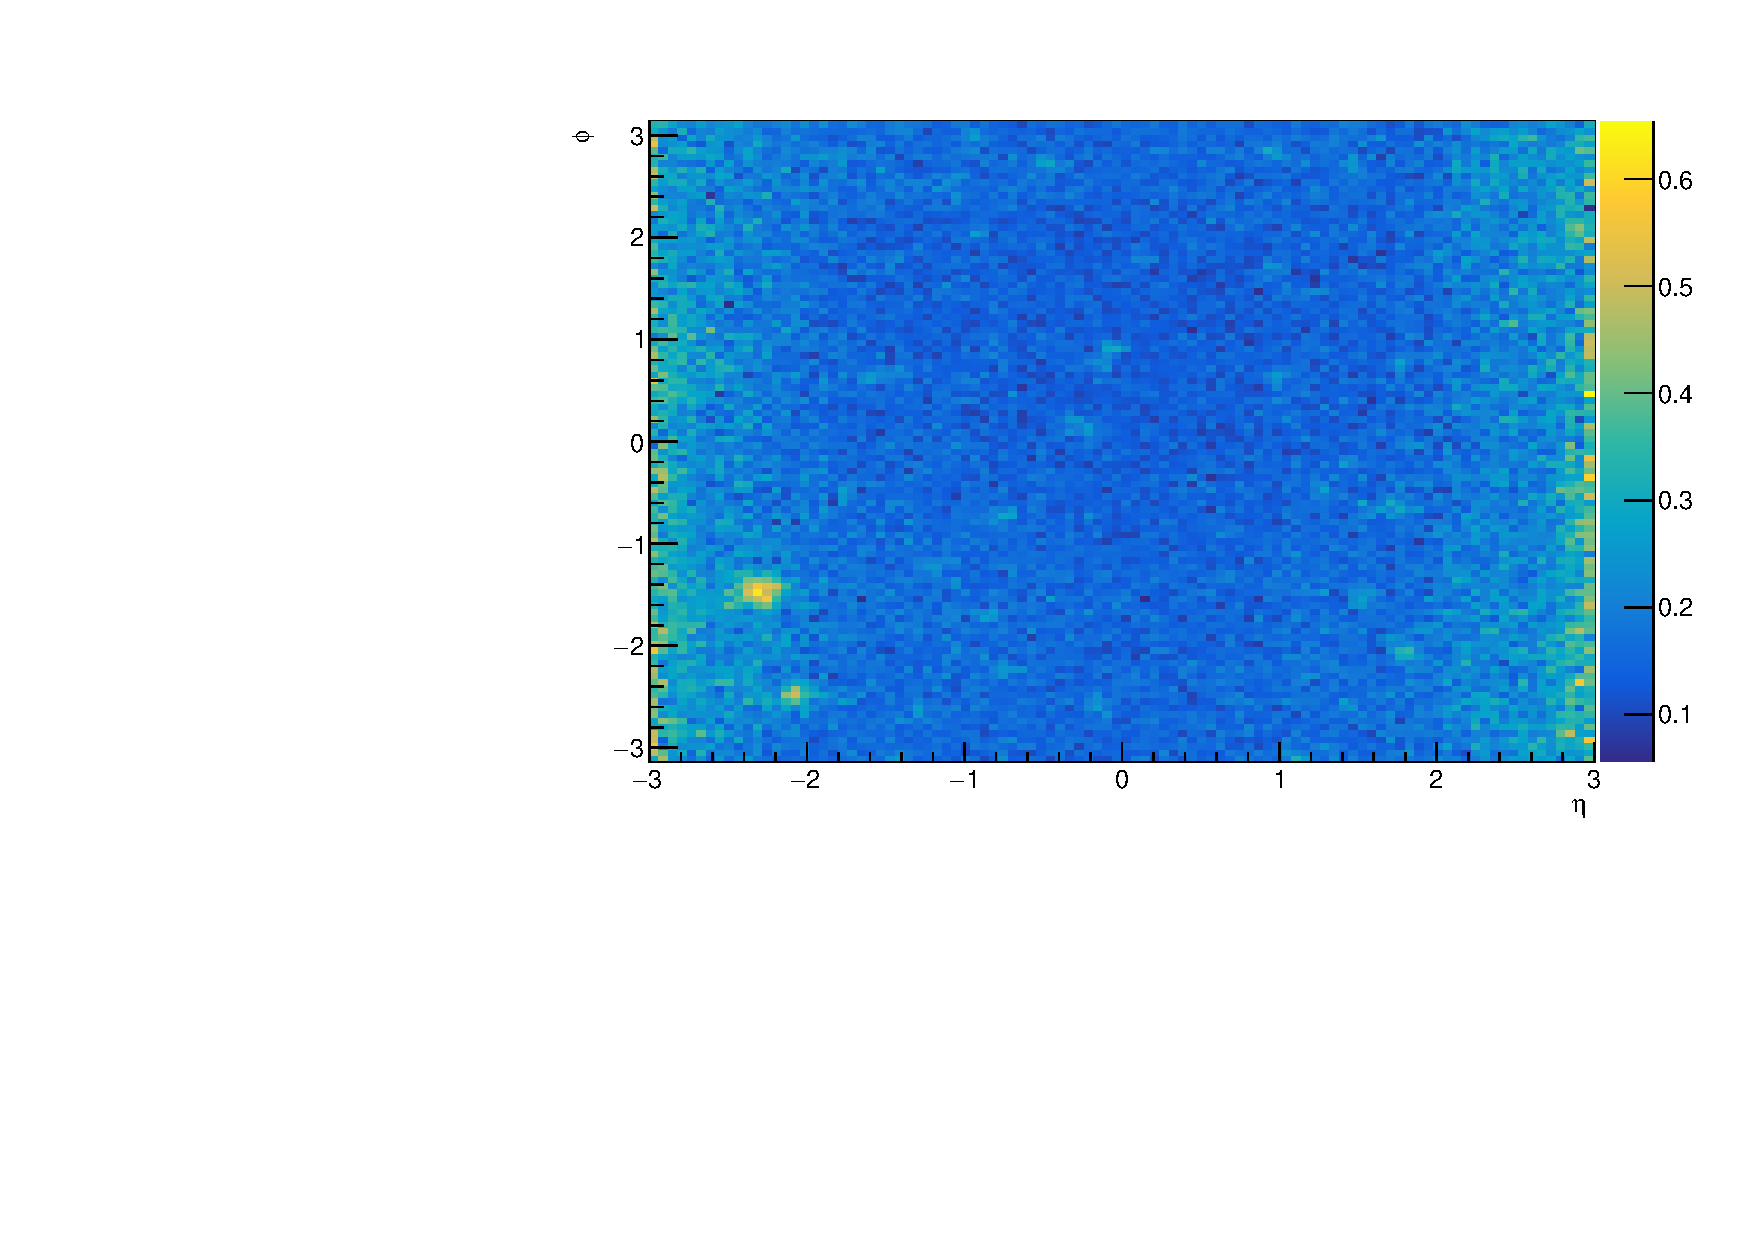
\includegraphics[width=0.7\textwidth]{figures/selection/EtaPhiMap.pdf}}
        \caption{2D ratio map, with unblinded signal region with luminosity of 149.49~$\text{pb}^{-1}$}
        \label{fig:2dRatioMap}
    \end{center}
\end{figure}



%To protect against severe energy losses caused by masked regions in the ECAL (which
%amount to about 1\% of the ECAL channel count) or HCAL, or by missing
%instrumentation in the barrel-endcap gap, events with $\bdphi < 0.5$
%are rejected if the distance in the ($\eta,\phi$) plane between the
%selected jet and the closest masked ECAL region, $\Delta R_{\rm
%  ECAL}$, is smaller than 0.3. Similarly, events are rejected if the
%jet points within 0.3 in $\eta$ of the ECAL barrel-endcap gap at
%$|\eta| = 1.5$.

{\bf Beam halo.}

The CSC beam halo filter has been found to be less efficient during the early
Run 2 data-taking period compared to the previous run.

Beam halo events manifest themselves as single energy deposits in the
calorimeters, which introduces large amounts of ``fake'' \met. This effect is
especially prominent in the signal region monojet category, particularly at
$\phi$ coordinates of 0 and $\pi$ because of the tendency of halo particles to
lie within the plane of the LHC ring. This is evident in
Fig.~\ref{fig:leadJetCleaning}.

Such spurious events are suppressed by requiring at least 10\% of the leading
jet's energy to originate from charged hadrons. The effectiveness of this selection
is demonstrated in Fig.~\ref{fig:leadJetCleaning}.

\begin{figure}[h!]
    \begin{center}
        {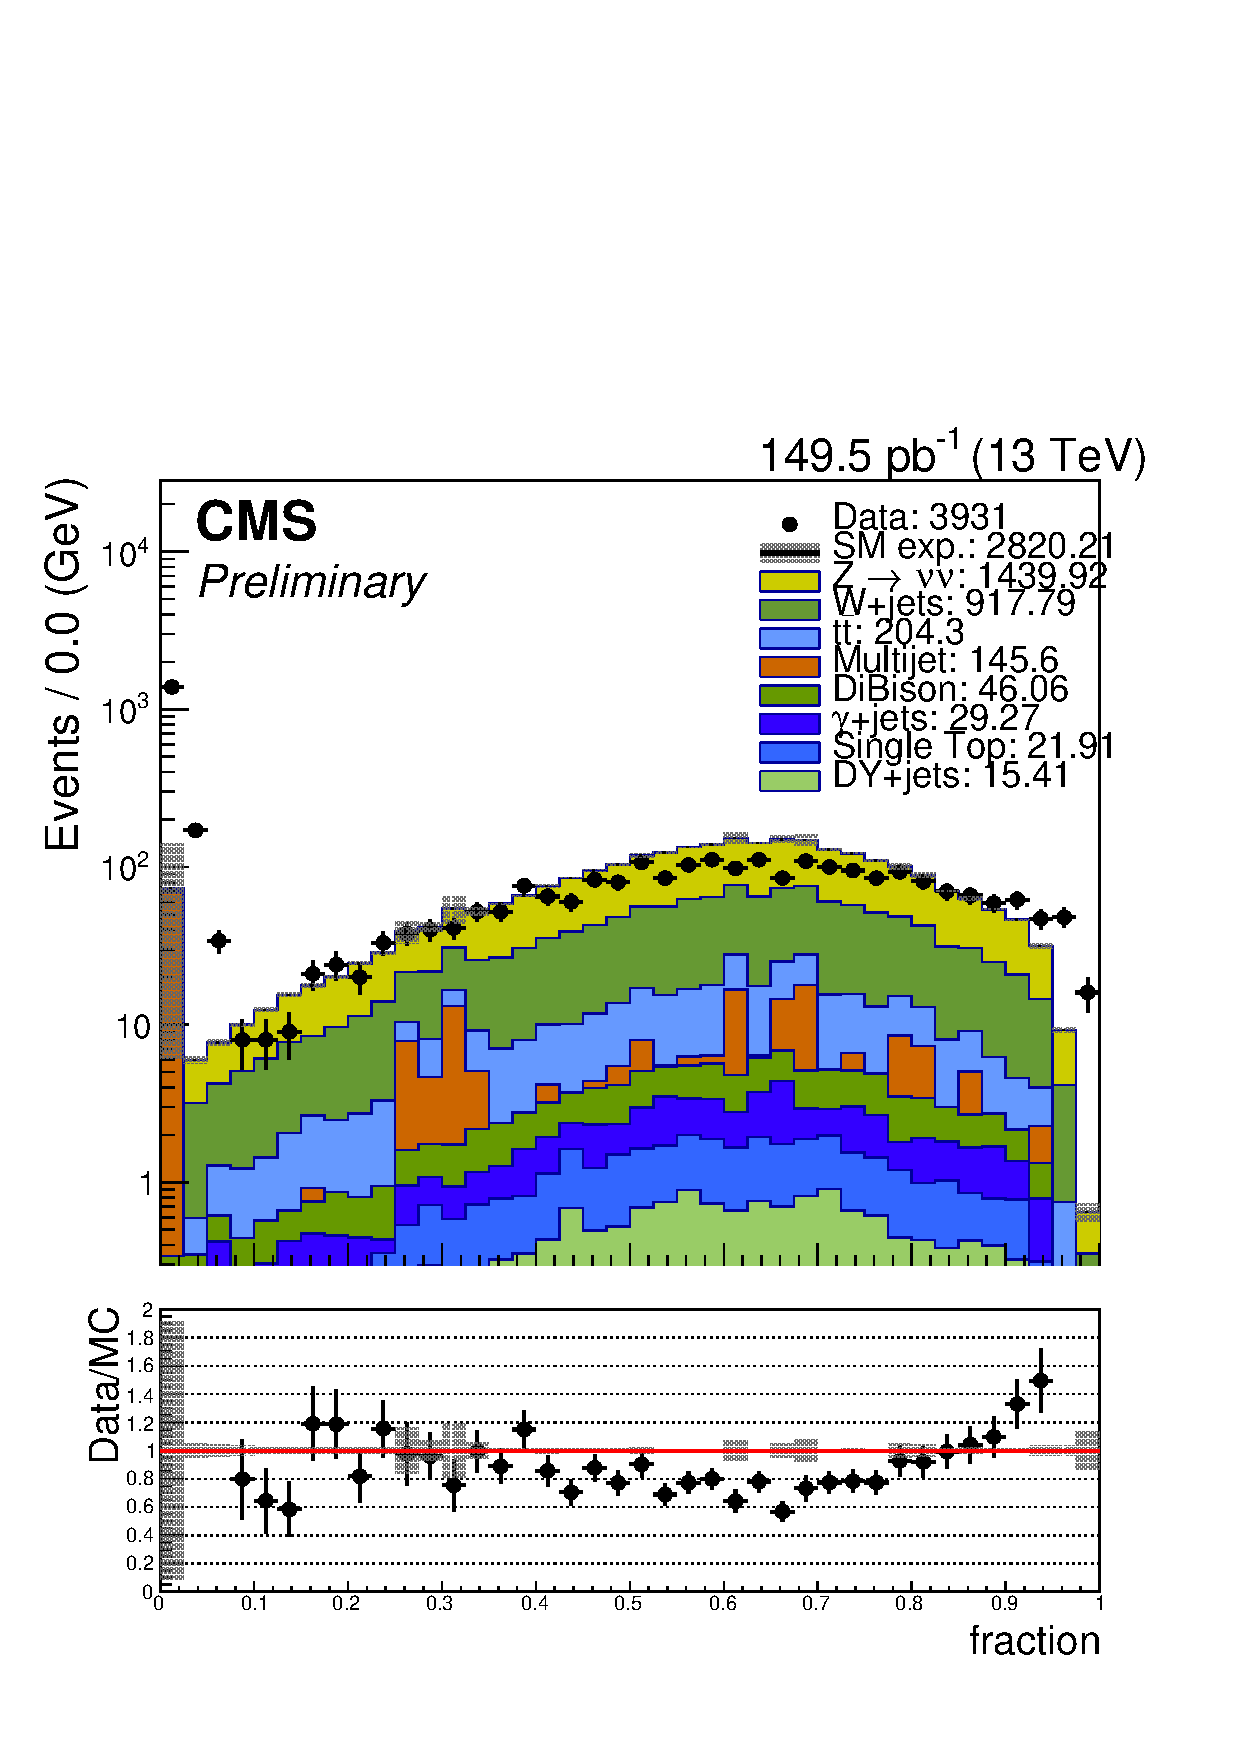
\includegraphics[width=0.32\textwidth]{figures/selection/leadJetChf_all_before.pdf}}
        {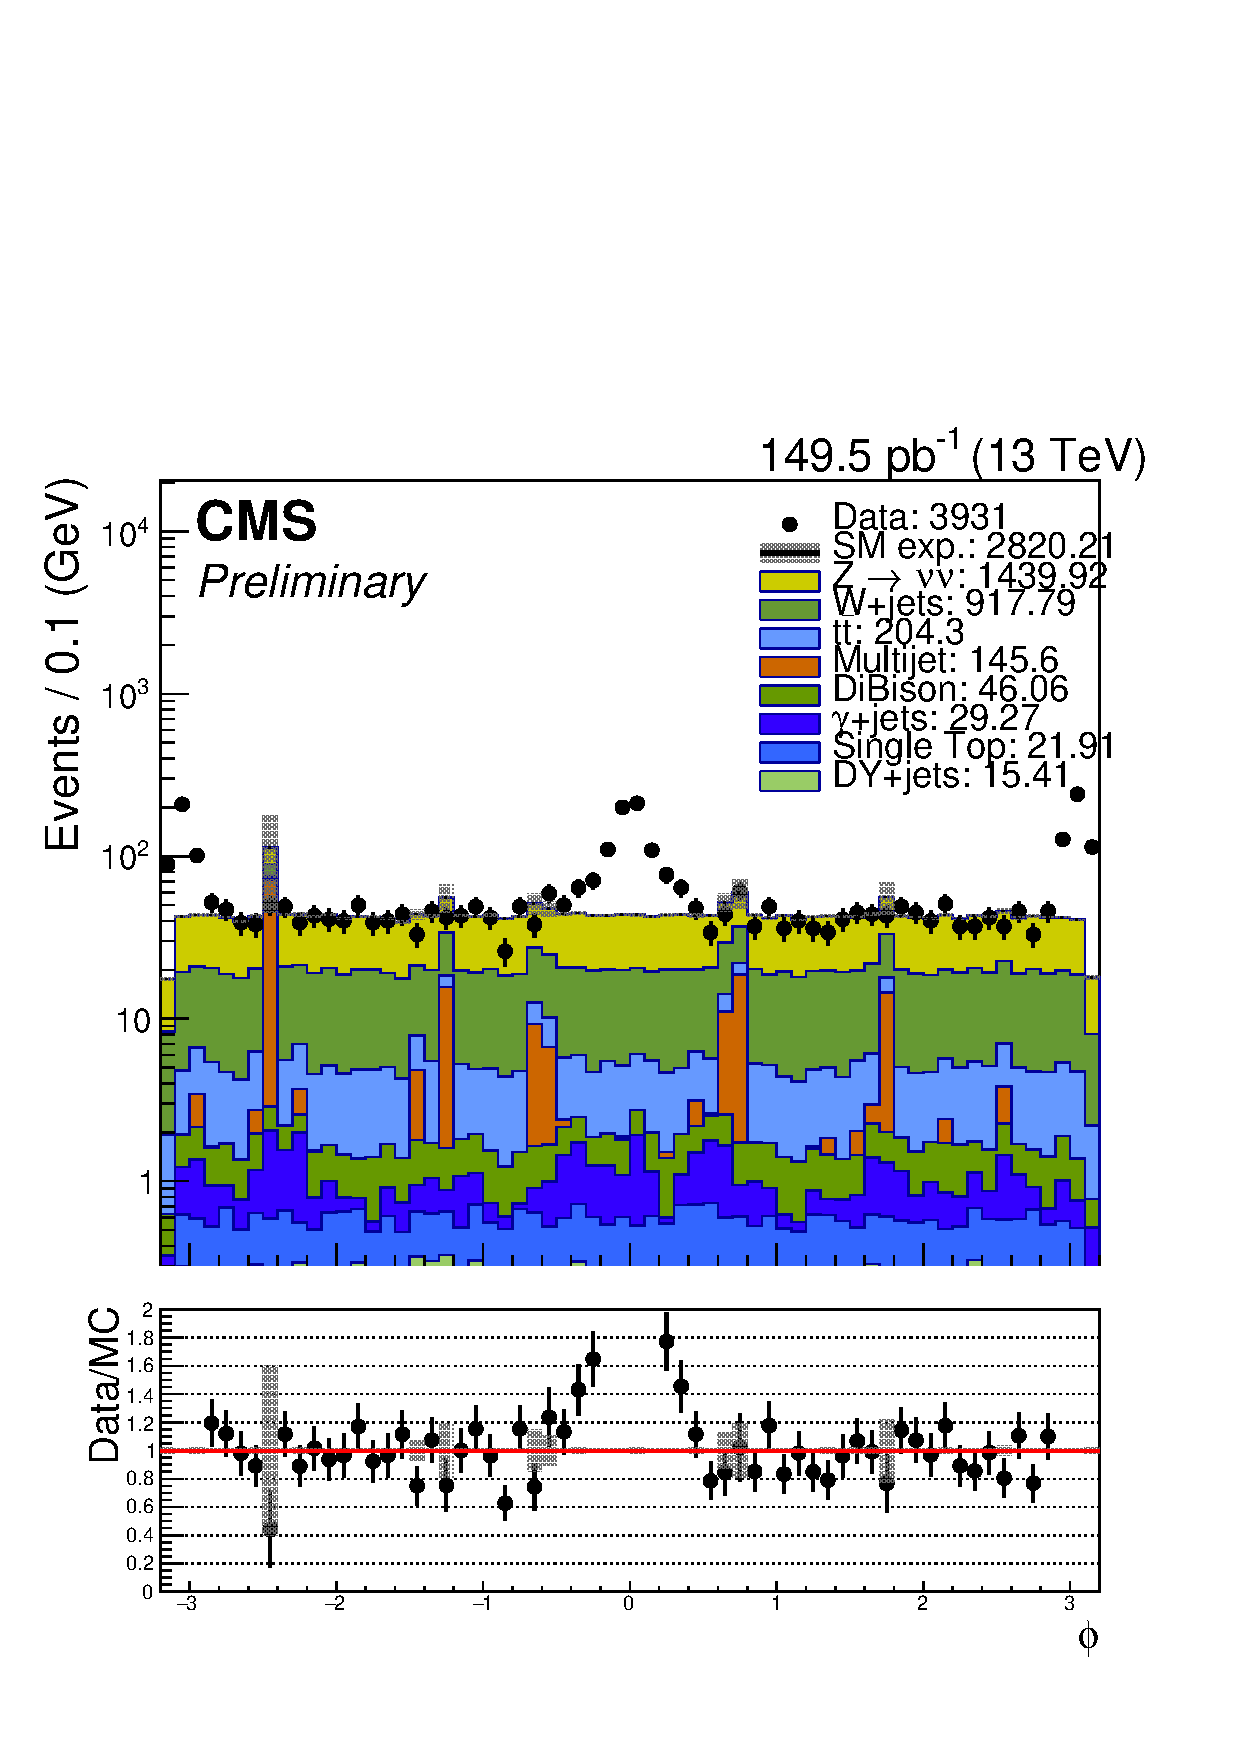
\includegraphics[width=0.32\textwidth]{figures/selection/leadJetPhi_all_before.pdf}}
        {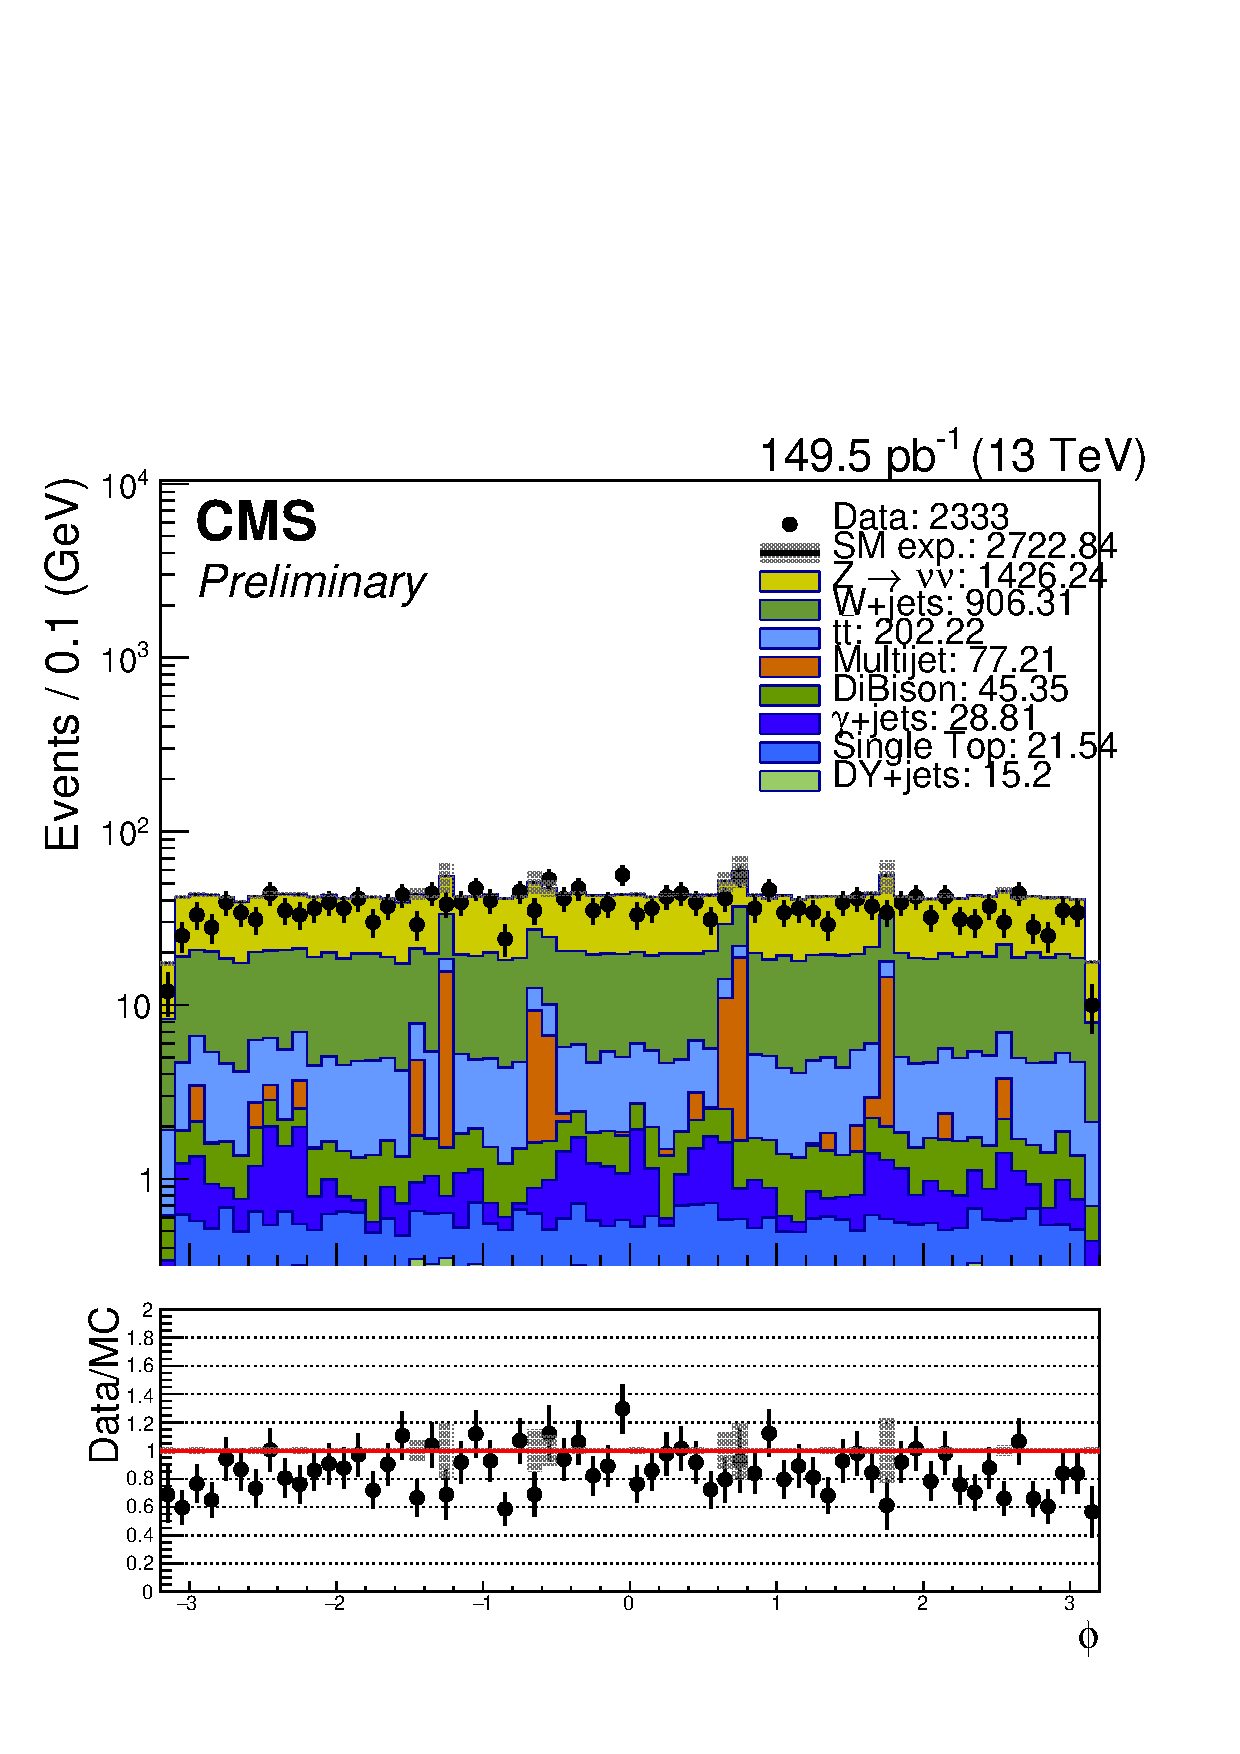
\includegraphics[width=0.32\textwidth]{figures/selection/leadJetPhi_all_after.pdf}}
        \caption{Distributions in the signal region of the lead jet charged hadron
        energy fraction (CHF) (Left), lead jet $\phi$ direction (Centre), and lead jet $\phi$
        direction after applying a requirement of {CHF~$>0.1$}. The large excess in data
        at charged hadron fractions close to zero and ${\phi = 0, \pi}$ is consistent with beam
        halo effects, and is effectively suppressed by the aforementioned selection.}
        \label{fig:leadJetCleaning}
    \end{center}
\end{figure}


{\bf Summary of signal region selection.} 

The requirements that define the hadronic signal region are summarised
in Table~\ref{tab:sr-selections}.

\begin{table}[h!]
  \topcaption{Summary of the signal region selection criteria, applied
    in addition to the pre-selection summarised in
    Table~\ref{tab:pre-selections}.}
  \label{tab:sr-selections}
  \centering
  \footnotesize
  \begin{tabular}{ ll }
    \hline
    \hline
    Selection             & Requirement                                                    \\
    \hline
    \alphat               & $>$0.52--0.65 (\HT-dependent) for region $200 < \HT < 800\gev$ \\
    \mht                  & $>130\gev$ for region $\HT > 800\gev$                          \\  
    \bdphi                & $>0.3$                                                         \\
    \mht/\met             & $<1.25$                                                        \\
    ``Dead ECAL filter''  & (see text)                                                     \\
    \hline
    \hline
  \end{tabular}
\end{table}

\subsection{Adding the \texorpdfstring{\mht}{MHT} dimension}
\label{sec:had-shape}

As described above, and as used in Run~1, the analysis takes advantage
of three discriminating variables, \njet, \nb, and \HT, to provide
sensitivity to a large range of SUSY (and DM) models. No extrapolation
in these variables is performed, with predictions of SM background
yields in the (\njet,\nb,\HT) bins of the signal region based on both
observed counts and transfer factors derived from simulated yields in
the corresponding (\njet,\nb,\HT) bins of the control samples. Each
prediction is statistically and systematically independent.

In Run~1, for each (\njet,\nb,\HT) bin in the signal region, an
extrapolation in the variable \alphat was necessary to obtain
background predictions based on the muon control samples, which did
not impose any \alphat requirement. No extrapolation in \alphat was
performed for the photon control sample, which used the same \alphat
requirements as the signal region. The \alphat requirements used in
Run~1 for the signal region correspond loosely to \mht thresholds in
the range $\sim$130 to $\sim$500\gev depending on the \HT
bin. Uncertainties in this extrapolation were determined through
closure tests with respect to data, including one dedicated to the
\alphat extrapolation, plus additional cross checks.

In Run~2, we will additionally bin event counts in the signal region
according to the variable \mht in order to provide further
discriminating power between any potential signal and the SM
background counts. Hence, while no extrapolation is performed in
\njet, \nb, nor \HT, the analysis will rely on information obtained
from simulation to extrapolate from counts (integrated over \mht) in
the control samples to a predicted distribution in \mht for each
corresponding (\njet,\nb,\HT) bin in the signal region.

The \mht dimension is included in the likelihood model using templates
determined per (\njet,\nb,\HT) bin from simulation. An associated
normalisation nuisance is determined from closure tests between
simulation and data, as described in
Sec.~\ref{sec:systematics}. Alternative templates are used to encode
the systematic uncertainty in the \mht distribution obtained from
simulation. 
%Preliminary studies and estimates of the shape systematics are also
%discussed Sec.~\ref{sec:systematics}. The likelihood model is
%described in Sec.~\ref{sec:likelihood}.

The templates use \mht bins of 50\gev in width. A metric is used to
determine the threshold of the final \mht bin used by the
templates. This metric is currently based on requiring a minimum
number of both observed counts in the {\it data control samples} and
(unweighted) simulated events with \mht values higher than the final
bin threshold. While the counts in the (\njet,\nb,\HT) bins of each
data control sample will not be binned according to \mht (as in the
signal region), the former requirement ensures that there are
sufficient events in each (\njet,\nb,\HT) bin of the control samples
to probe for potential systematic effects {\it across all bins in
  \mht} using closure tests between simulation and data, as described
in Sec.~\ref{sec:systematics}. Hence, a data-driven cross check for
potential biases and on the systematic uncertainty in the \mht
template is possible. The latter requirement minimises the statistical
uncertainties associated with the finite number of simulated events
for the various SM background processes. Both requirement are based on
counts according to \njet and \nb but inclusive with respect to \nb.

\subsection{The hadronic control region}

A hadronic control region that is enriched in multijet events and
disjoint with respect to the signal region is obtained by applying
both the pre-selection criteria and lepton/photon vetoes, as defined
above, and inverting the (\HT-dependent) \alphat and/or \mhtmet
requirements. 
%None of the cleaning filters are not applied to allow the study of
%instrumental effects. 
The sample of events populating this control region are used primarily
to estimate any residual background contamination from QCD multijet
events, described in Sec.~\ref{sec:qcd}.

\subsection{Commonalities between the data control regions}

There are five control regions with leptons or photons in the final
state: \mj, \mmj, \ej, \eej, and \gj. The full pre-selection is
applied as part of the definition of each of these control
regions. The cuts on event-level jet-based quantities are identical to
those applied in the hadronic search region and the same \njet, \nb,
and \scalht binning is used. The lepton(s) or photon is not considered
in the calculation of the event-level variables.

The selection criteria of the various control regions are defined such
that the background composition and event kinematics of the control
regions mirror as closely as possible those for the signal
region. This is done in order to minimise the reliance on the
simulation to model correctly the backgrounds and event kinematics in
the control and signal samples.

Two exceptions are made. First, no \bdphi requirement is imposed as
part of the selection criteria defining the control regions. Second,
in the case of the four leptonic control regions, no requirement is
made on \alphat. This is made possible by the remaining kinematic
selection criteria, which are sufficiently selective to ensure that
the leptonic event samples remain rich in events from the \wj, \ttbar
and \zll processes with negligible contamination from QCD multijet
events. Thus, the acceptance of the leptonic control regions can be
significantly increased, which simultaneously improves their
predictive power and further reduces the effect of any potential
signal contamination.

The lepton event samples can be used to predict components of the SM
background across all \scalht bins, while the \gj sample can only be
used for the region $\HT > 400\gev$ due to the photon trigger
requirements.

\subsection{The \texorpdfstring{\mj}{muon plus jets} control sample}
\label{subsec:mucontrolSelection}

%Events from the \wj and \ttbar processes are found in the hadronic
%signal sample due to unidentified leptons (either out of acceptance or
%not reconstructed) and hadronic tau decays originating from
%high-p$_{T}$ W bosons. An estimate of these background processes is
%obtained through the use of a \mj sample. 

The selection criteria for the \mj sample are chosen to identify W
bosons decaying to a muon and a neutrino in the phase-space of the
signal. In order to select events containing W bosons, exactly one
tight isolated muon within an acceptance of \PT $>$ 30 \gev and
$|\eta| <$ 2.1 is required (due to the trigger), and the transverse
mass of the W candidate must satisfy $30 < \mt(\mu,\pfmet) < 125\gev$
(to suppress QCD multijet and potential signal events). Events are
vetoed if $\Delta R(\mu,\textrm{jet}_i) < 0.5$ running over all jets
$i$. The single isolated track veto, described in
Sections~\ref{sec:objects} and~\ref{sec:vetoes}, is also applied,
which considers all single isolated tracks in the event except that
associated with the identified, isolated muon. Finally, the cleaning
cut $\mht/\met$ is also applied, as done in the signal region, where
the \met is adjusted to account for the transverse momentum of the
identified, isolated muon.

\subsection{The \texorpdfstring{\mmj}{di-muon plus jets} control sample}

%The \znunu\ + jets process forms an irreducible background and can be
%estimated using the \zmumu + jets process, which has similar kinematic
%properties but a different acceptance and a smaller branching ratio. A
%background estimate is obtained through the use of a \mmj sample. 

The selection criteria are identical to those for the \mj sample, with
the following exceptions that are tuned to identify Z bosons decaying
to two muons in the kinematic phase space of the signal region. 
In order to select an event sample containing Z bosons, exactly two
tight isolated muons within an acceptance of $\Pt > 30\gev$ and
$|\eta| < 2.1$ are required (due to the trigger). The invariant mass
of the two muons must satisfy $m_{Z} - 25 < M_{\mu_1\mu_2} < m_{Z} +
25$ and they must have opposite charge. Events are vetoed if $\Delta
R(\mu_{i},\textrm{jet}_j) < 0.5$ is satisfied, running over all muons
$i$ and all jets $j$. The single isolated track veto is also applied
considering all single isolated tracks in the event except those
associated with the two identified, isolated muons. Finally, the
cleaning cut $\mht/\met$ is also applied, as done in the signal
region, where the \met is adjusted to account for the transverse
momenta of the two identified, isolated muons. 

\subsection{The \texorpdfstring{\ej}{electron plus jets} control sample}
\label{subsec:elecontrolSelection}

The selection criteria that define the \ej control sample
mirror those of the \mj sample, \ie, they are tuned
to identify W boson decaying to an electron and a neutrino in the
kinematic phase space of the signal region.

Electrons are required to satisfy the Tight working point and satisfy
the requirements $\Pt> 30\gev$ and $|\eta| < 2.1$. The tightening of
the Loose working point defined in Sec.~\ref{sec:electron-id} was
found to greatly reduce multijet contamination without a large
reduction in statistics within the electron control samples. The
transverse mass of the W candidate must satisfy $30 < \mt(e,\pfmet)
< 125\gev$.

\subsection{The \texorpdfstring{\eej}{electron plus jets} control sample}
\label{subsec:dielecontrolSelection}

The selection criteria that define the \eej control sample
mirror those of the \mmj sample. They are tuned
to identify Z boson decaying to a pair of electrons in the
kinematic phase space of the signal region.

Both electrons need to satisfy Tight working point and the
requirements $\Pt> 30\gev$ and $|\eta| < 2.1$. The invariant mass of
the two electrons must satisfy $m_{Z} - 25 < M_{e_1e_2} < m_{Z} + 25$
and they must have opposite charge.

\subsection{The \texorpdfstring{\gj}{photon plus jets} control sample}
\label{subsec:photoncontrolSelection}

%The \znunu\ + jets process can also be estimated using the \gj
%process, which has a larger cross section and kinematic properties
%similar to those of \znunu\ events when the photon is
%ignored~\cite{PAS-SUS-08-002,Bern:2011pa}. 

The \gj sample is defined by requiring exactly one photon satisfying
tight isolation criteria and within an acceptance of $\pt > 200\gev$
(limited by trigger requirements) and $|\eta| < 1.45$. Furthermore,
events are vetoed if $\Delta R(\gamma,\textrm{jet}_i) < 1.0$ is
satisfied, running over all jets $i$. One important difference with
respect to the leptonic control samples is the application of the
\HT-dependent \alphat requirements imposed as part of the signal
region definition. This is done primarily to ensure that the photon
control sample and signal region are subject to identical kinematic
requirements and the photon carries sufficient transverse energy so
that the mass of the Z boson becomes a negligible effect when using
the \gj sample to predict the kinematic distributions of the \znunu
background. The cleaning cut $\mht/\met$ is also applied, as done in
the signal region, where the \met is adjusted to account for the
transverse energy of the identified, isolated photon. As stated above,
the \gj sample can only be used to predict background components in
the region $\HT > 400\gev$ due to trigger requirements.

%%____________________________________________________________________________||
\section{Expected event yields}
\label{sec:yields}

%%____________________________________________________________________________||
% \subsection{Key distributions for the hadronic signal
%   region\label{sec:mc-data-comp}}
%
% %Distributions of key analysis variables 
% The hadronic signal region selection is detailed in Sec.~\ref{sec:hadSelection}.

%%____________________________________________________________________________||
\subsection{Breakdown of SM backgrounds in the hadronic signal
  region\label{sec:bkgd-comp}}

In the absence of multijet events from QCD, the remaining significant
backgrounds in the signal region are expected to stem from SM
processes with genuine \met in the final state. For the low jet
multiplicity categories, the largest backgrounds with genuine \met are
generally from the associated production of W or Z bosons with jets,
followed by either the weak decays \znunu\ or \wtaunu, where the
$\tau$ decays hadronically and is identified as a jet, or by leptonic
decays that are outside acceptance or not rejected by the dedicated
electron or muon vetoes. For the higher jet multiplicity categories,
top quark production followed by semileptonic weak top quark decay
becomes important. The relative contribution from \ttbar is enhanced
or suppressed depending on the number of b-jets required. 
% A breakdown
% of the relative contributions of the SM backgrounds, as given by
% simulation, in the different (\njet, \nb, \scalht) bins can be found
% in Table~\ref{tab:backgrounds}. 
Plots showing the yields for these electroweak backgrounds and a reference
signal model can be seen in Figs~\ref{fig:ewkYields1}-\ref{fig:ewkYields4}. 
A breakdown of the three
dominant channels, \ttbar, \zInv~ and W~+~jets, are shown. The contribution from
other sources, such as the single top and diboson channels, was found to be
negligible so are not shown.

\begin{figure}[]
  \centering
  \subfigure[Hadronic signal region yields for electroweak backgrounds
  ($\njet = 2$)]{
    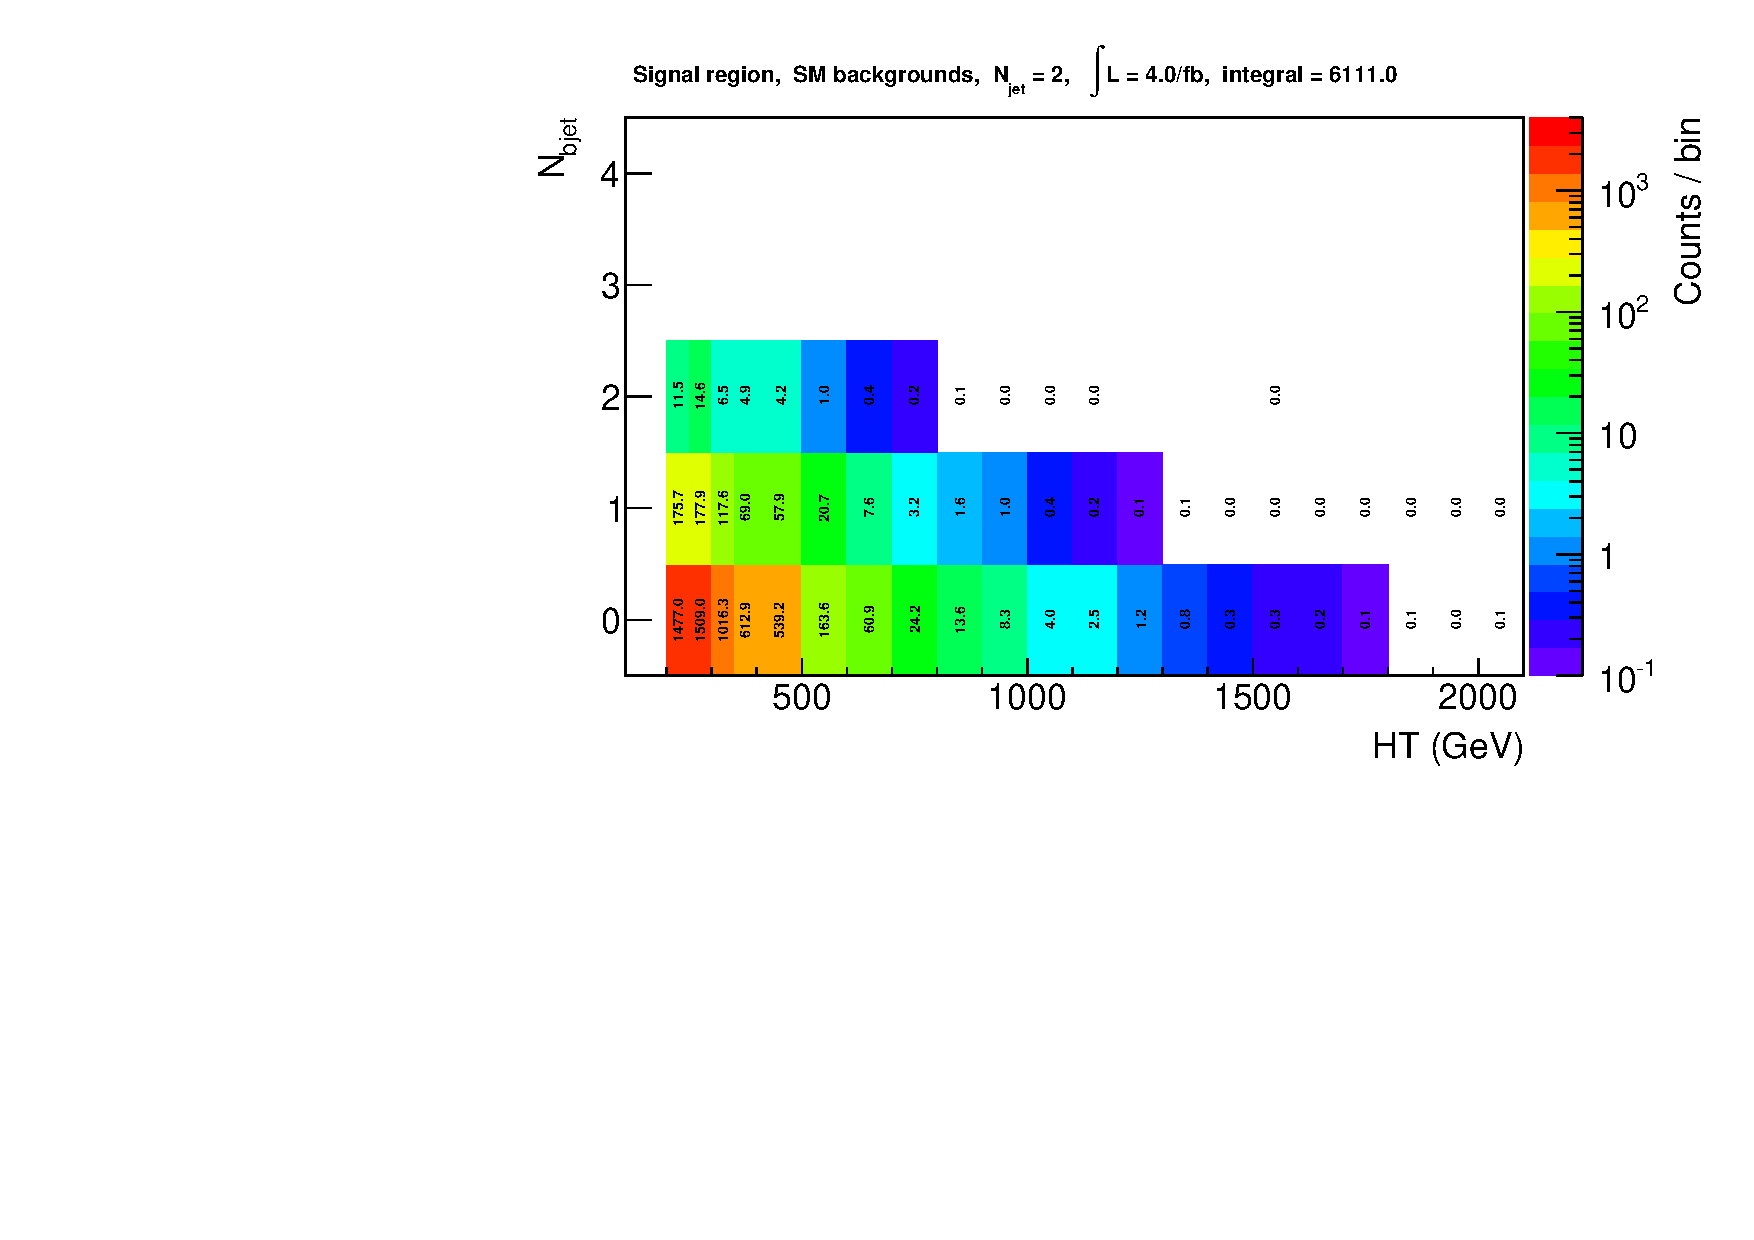
\includegraphics[width=0.5\textwidth]{figures/yieldPlots/had_ewk_eq2j.pdf}
  }~~
  \subfigure[Hadronic signal region yields for the \zInv background
  ($\njet = 2$)]{
    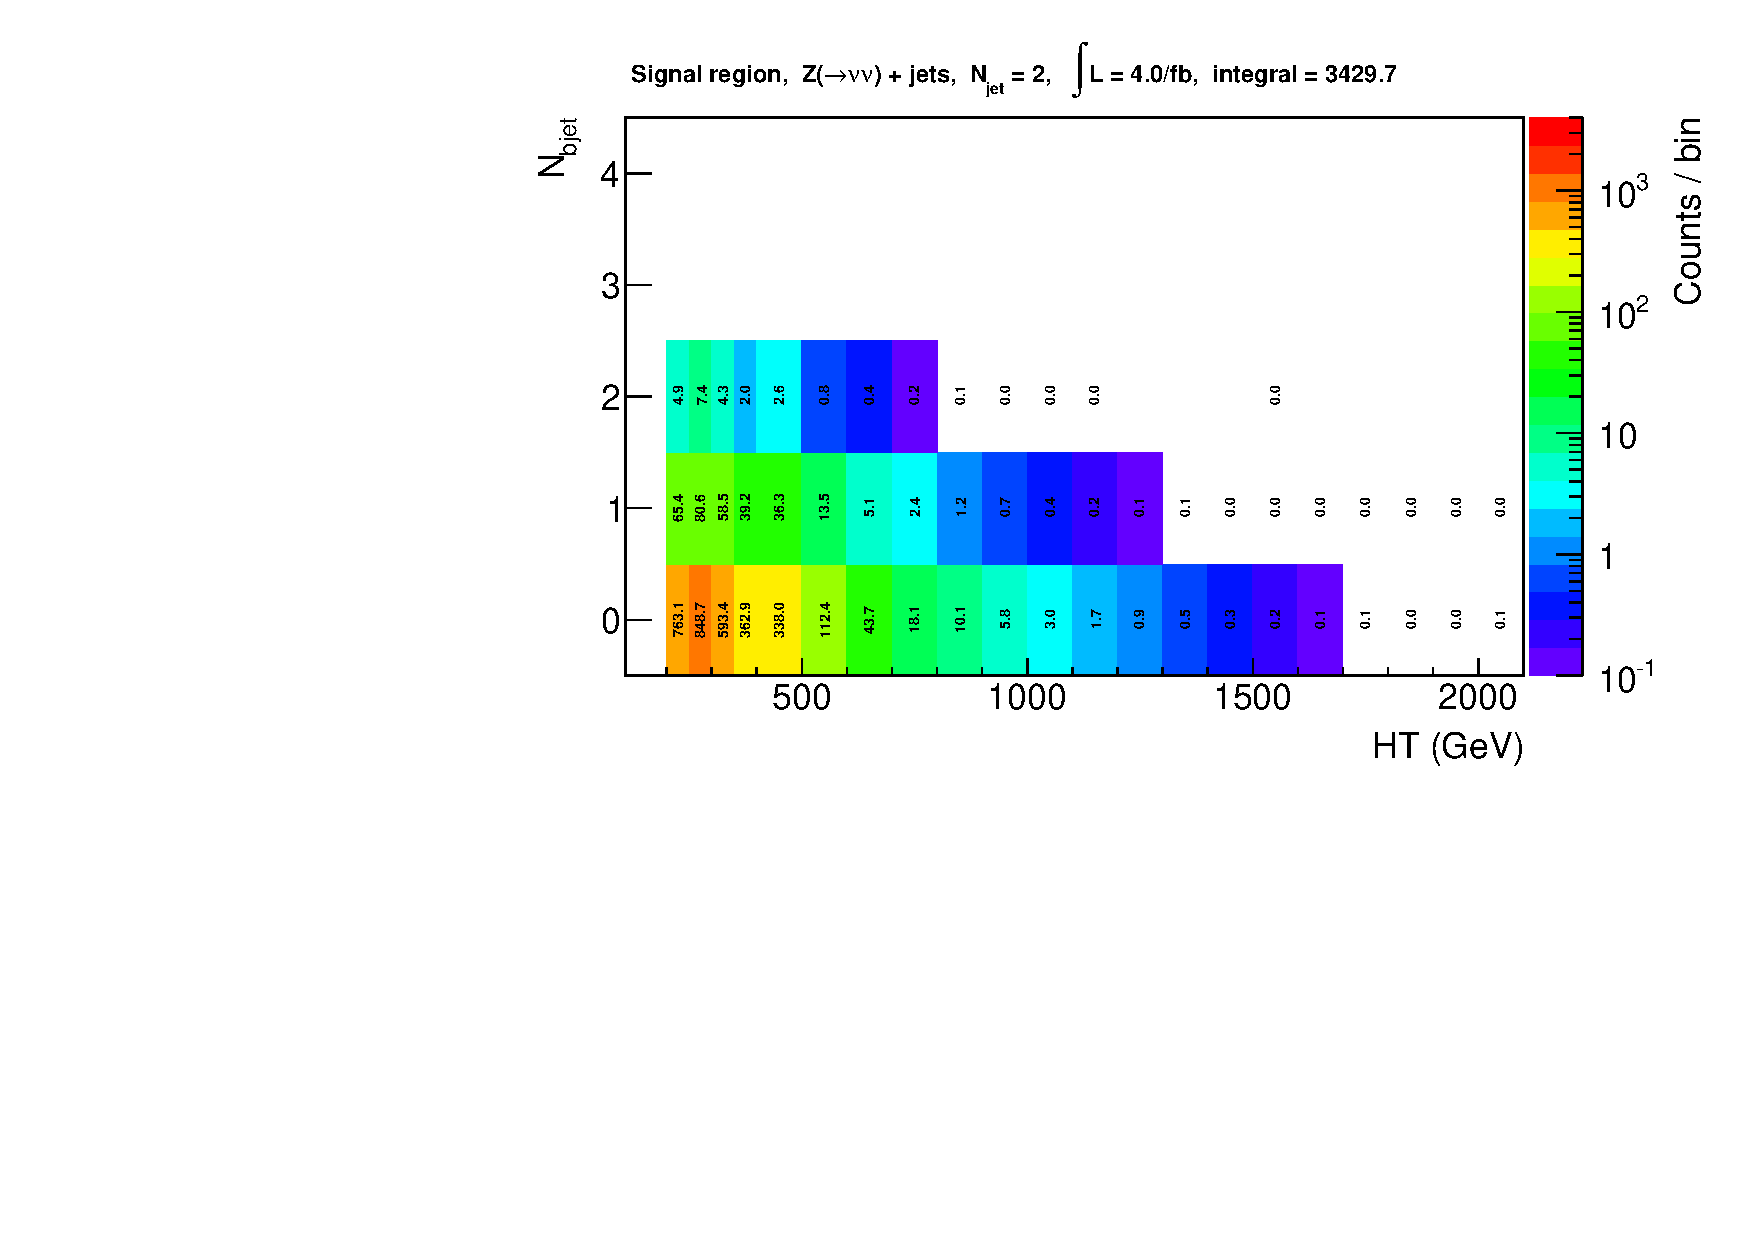
\includegraphics[width=0.5\textwidth]{figures/yieldPlots/had_zinv_eq2j.pdf}
  }\\
  \subfigure[Hadronic signal region yields for W~+~jets background
  ($\njet = 2$)]{
    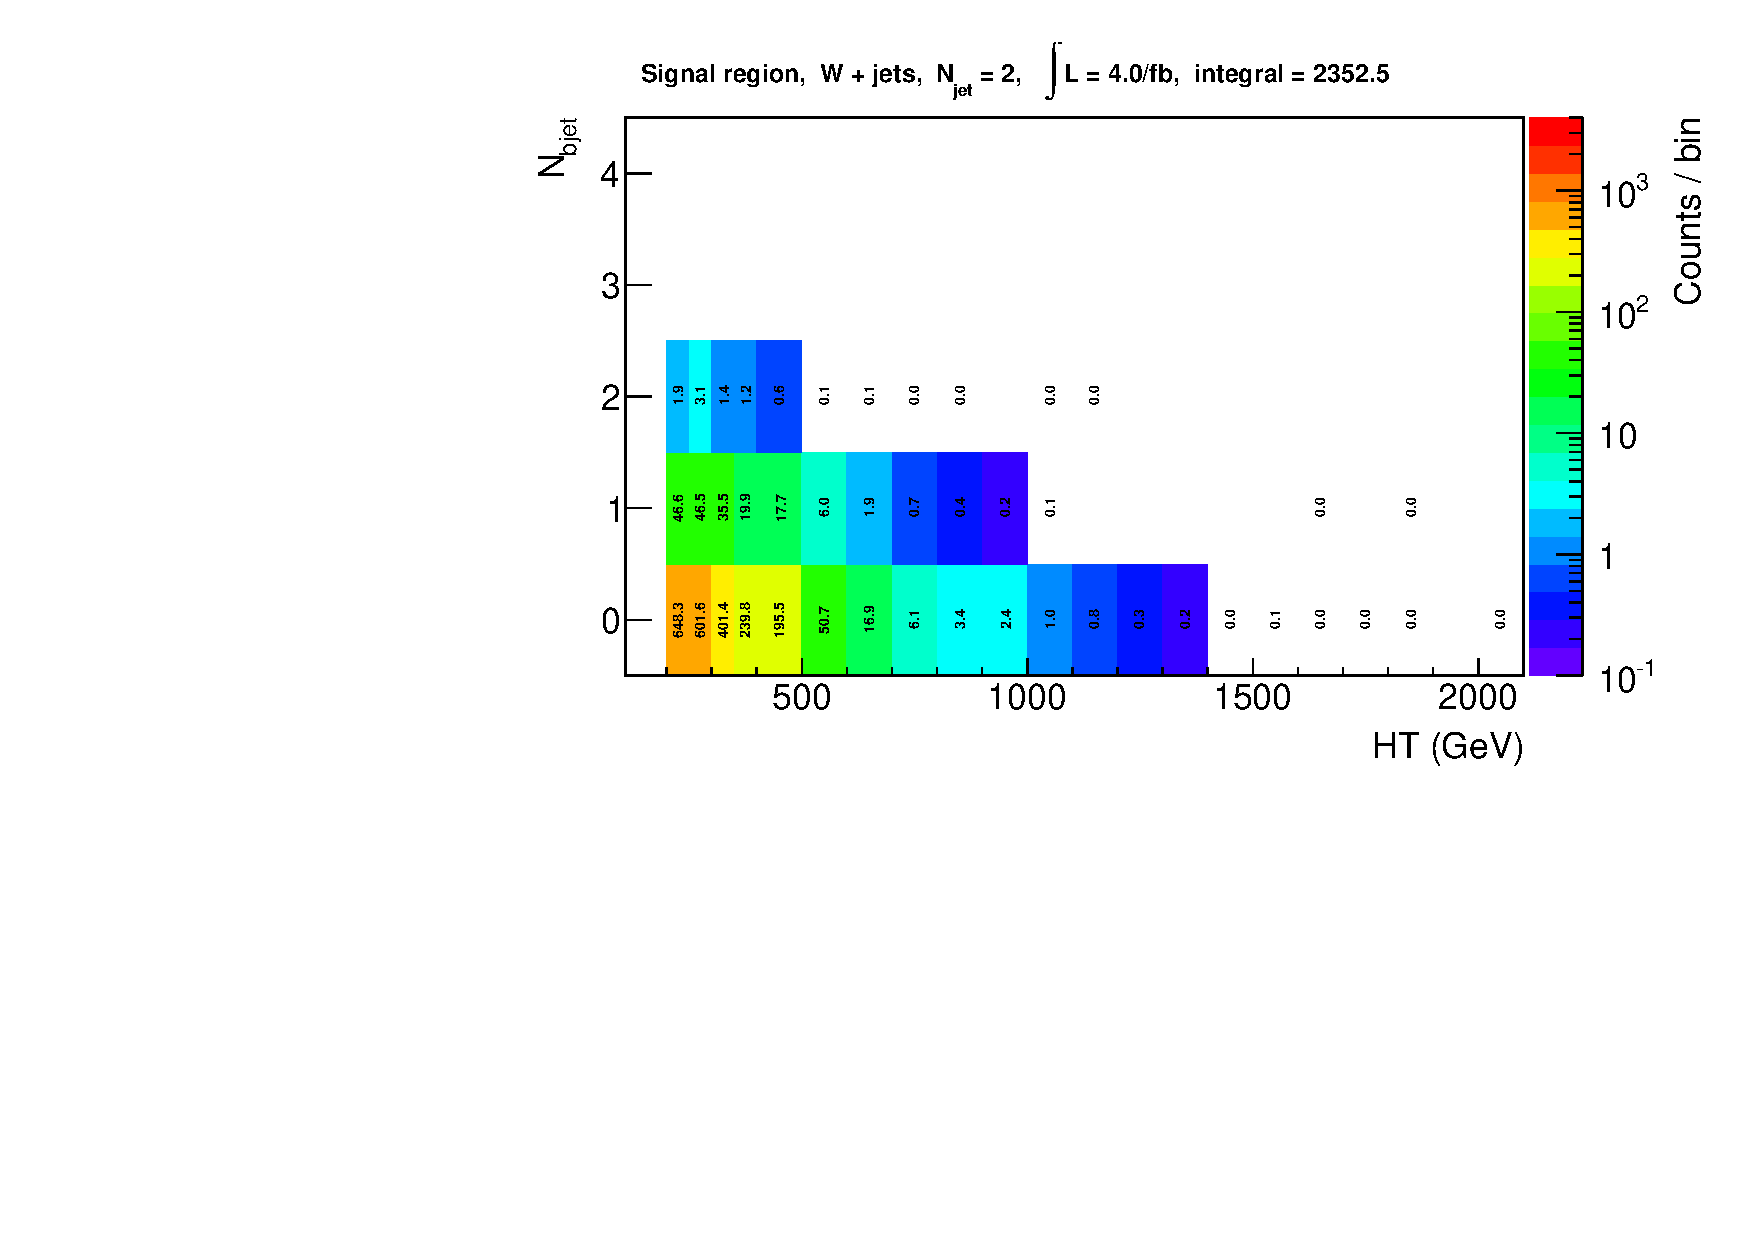
\includegraphics[width=0.5\textwidth]{figures/yieldPlots/had_wjets_eq2j.pdf}
  }~~
  \subfigure[Hadronic signal region yields for \ttbar background
  ($\njet = 2$)]{
    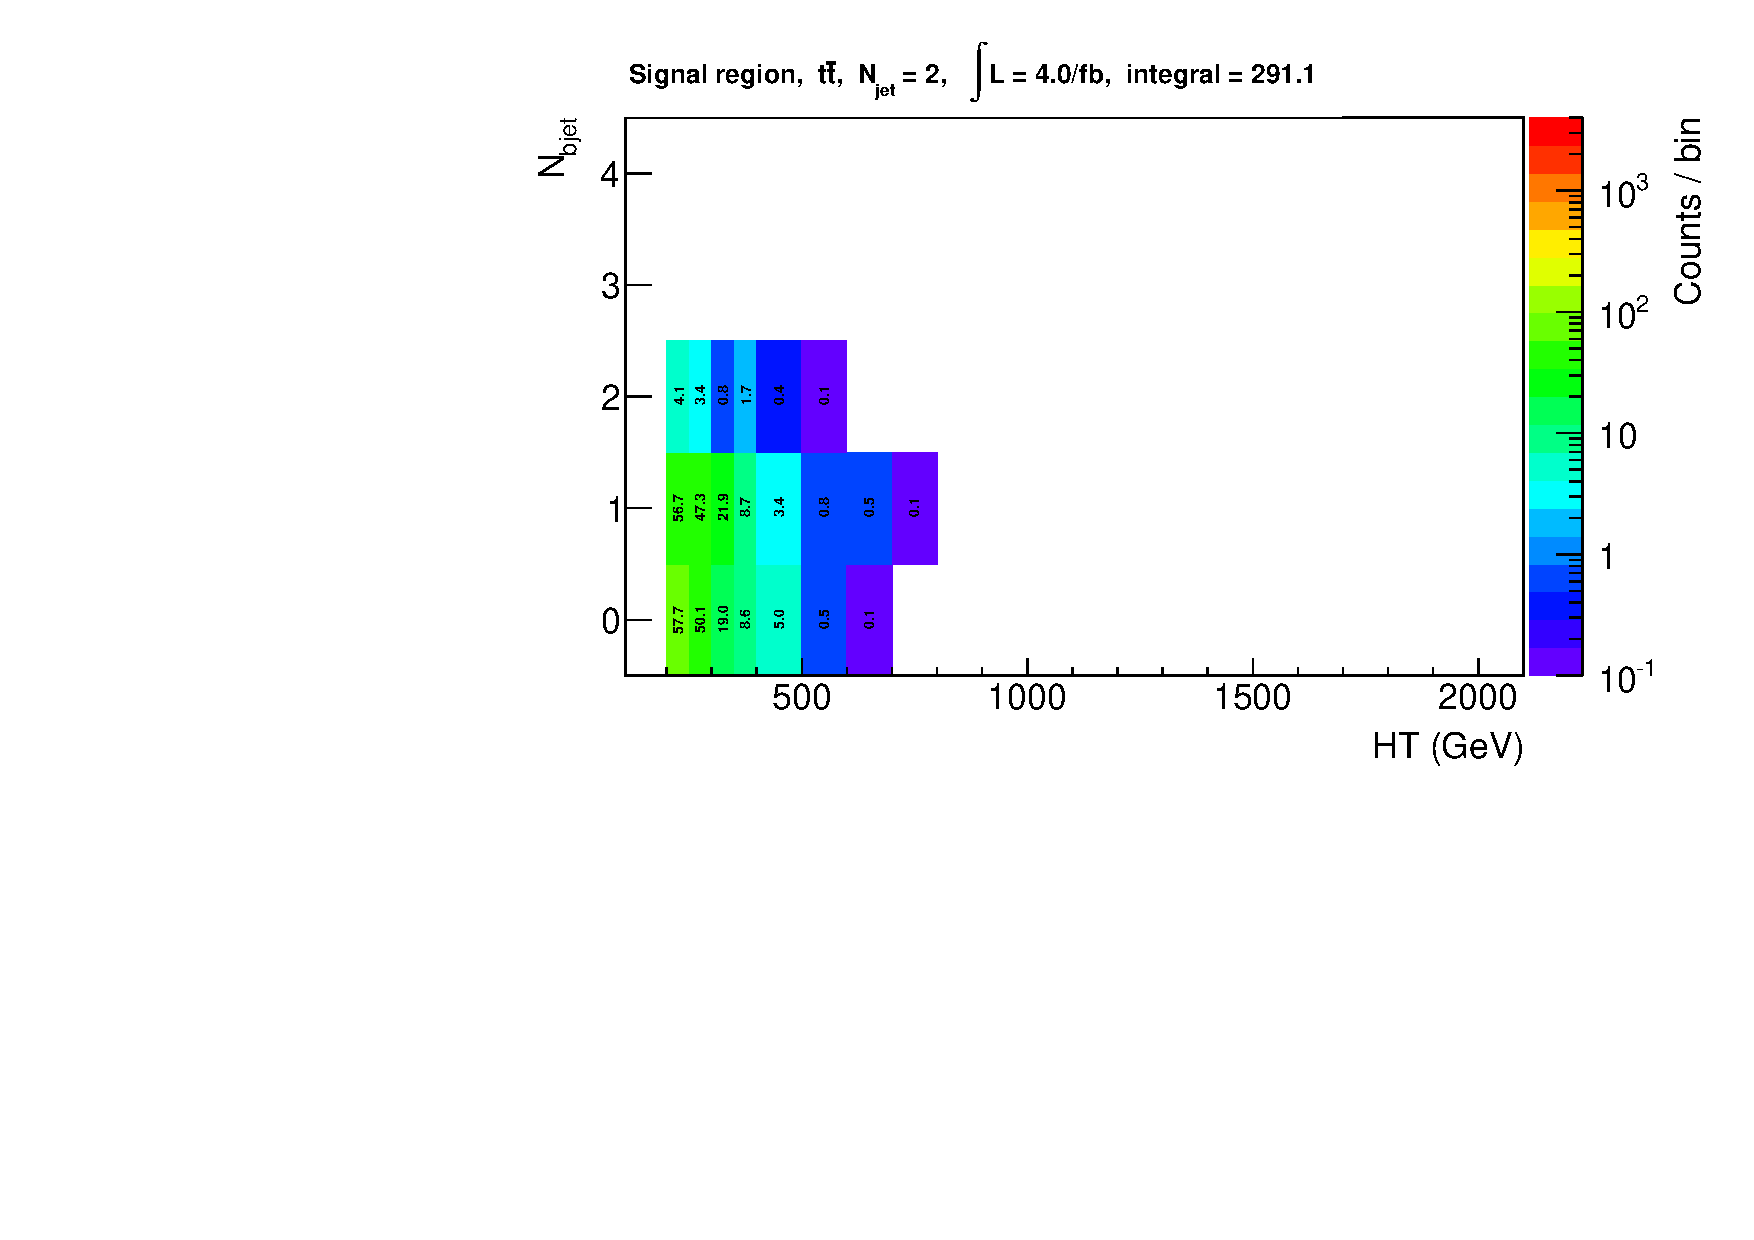
\includegraphics[width=0.5\textwidth]{figures/yieldPlots/had_ttbar_eq2j.pdf}
  }
  \caption{\label{fig:ewkYields1} Yields at $4\fbinv$ for the electroweak backgrounds in the
  hadronic signal region, $\njet=2$. The binning is chosen to be in line with the analysis
  bins. The contribution from the dominant backgrounds is shown separately.}
\end{figure}
\begin{figure}[]
  \centering
  \subfigure[Hadronic signal region yields for electroweak backgrounds
  ($\njet = 3$)]{
    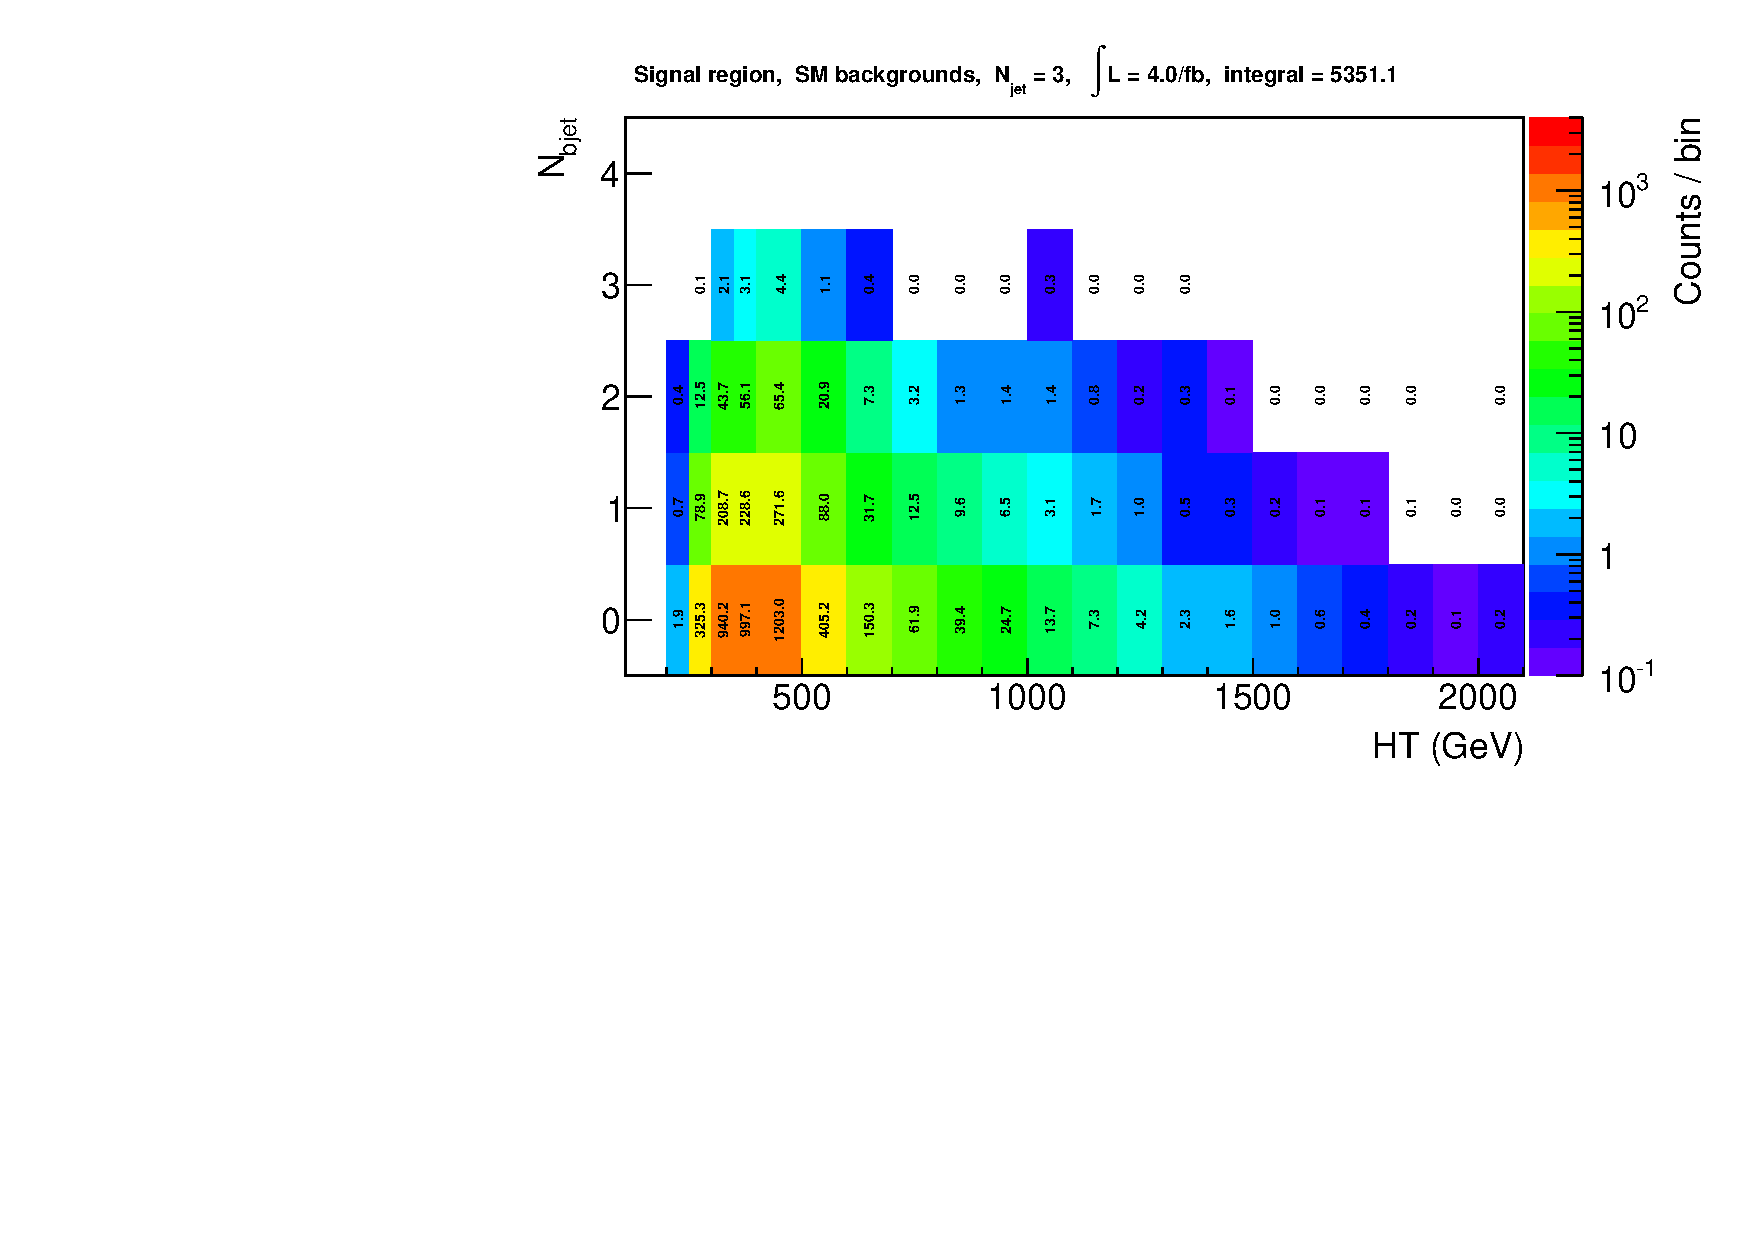
\includegraphics[width=0.5\textwidth]{figures/yieldPlots/had_ewk_eq3j.pdf}
  }~~
  \subfigure[Hadronic signal region yields for the \zInv background
  ($\njet = 3$)]{
    \includegraphics[width=0.5\textwidth]{figures/yieldPlots/had_zInv_eq3j.pdf}
  }\\
  \subfigure[Hadronic signal region yields for W~+~jets background
  ($\njet = 3$)]{
    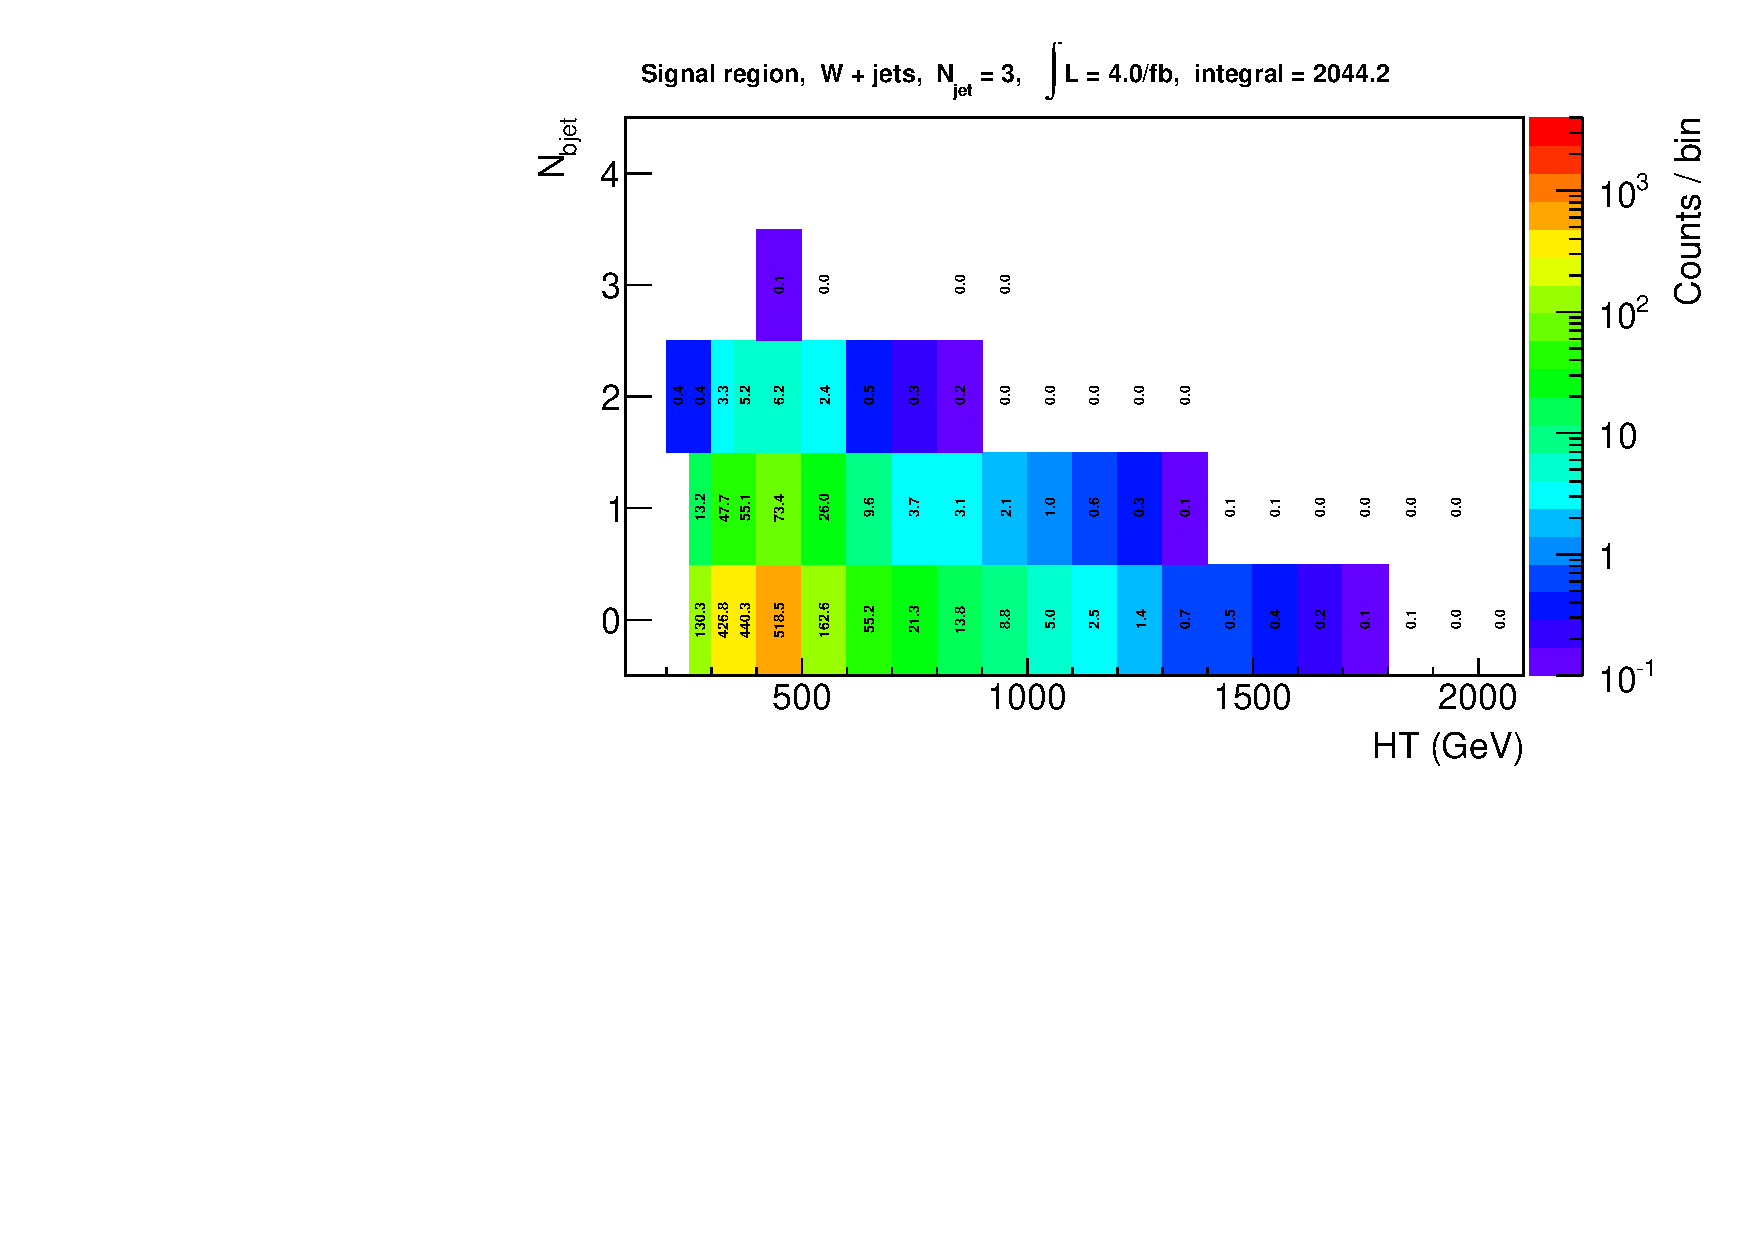
\includegraphics[width=0.5\textwidth]{figures/yieldPlots/had_wjets_eq3j.pdf}
  }~~
  \subfigure[Hadronic signal region yields for \ttbar background
  ($\njet = 3$)]{
    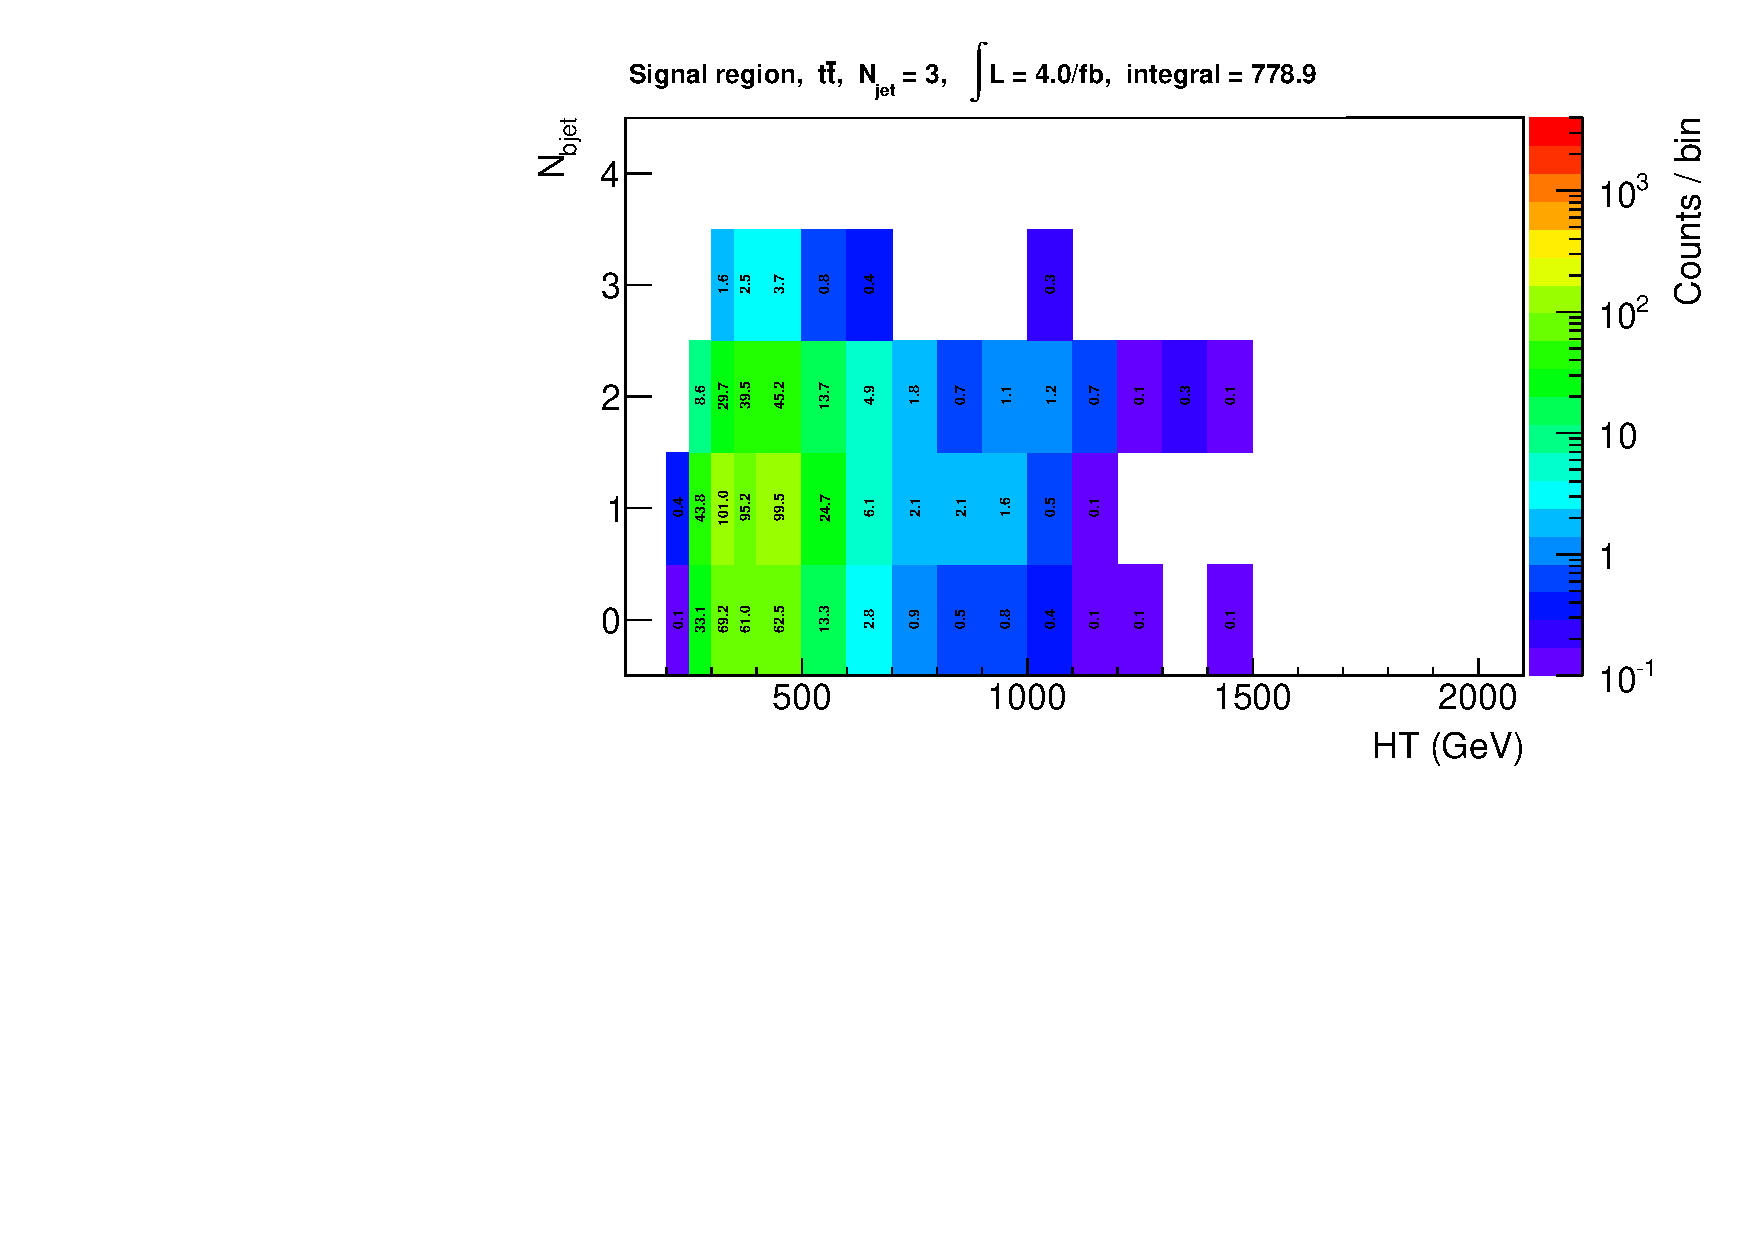
\includegraphics[width=0.5\textwidth]{figures/yieldPlots/had_ttbar_eq3j.pdf}
  }
  \caption{\label{fig:ewkYields2} Yields at $4\fbinv$ for the electroweak backgrounds in the
  hadronic signal region, $\njet=3$. The binning is chosen to be in line with the analysis
  bins. The contribution from the dominant backgrounds is shown separately.}
\end{figure}
\begin{figure}[]
  \centering
  \subfigure[Hadronic signal region yields for electroweak backgrounds
  ($\njet = 4$)]{
    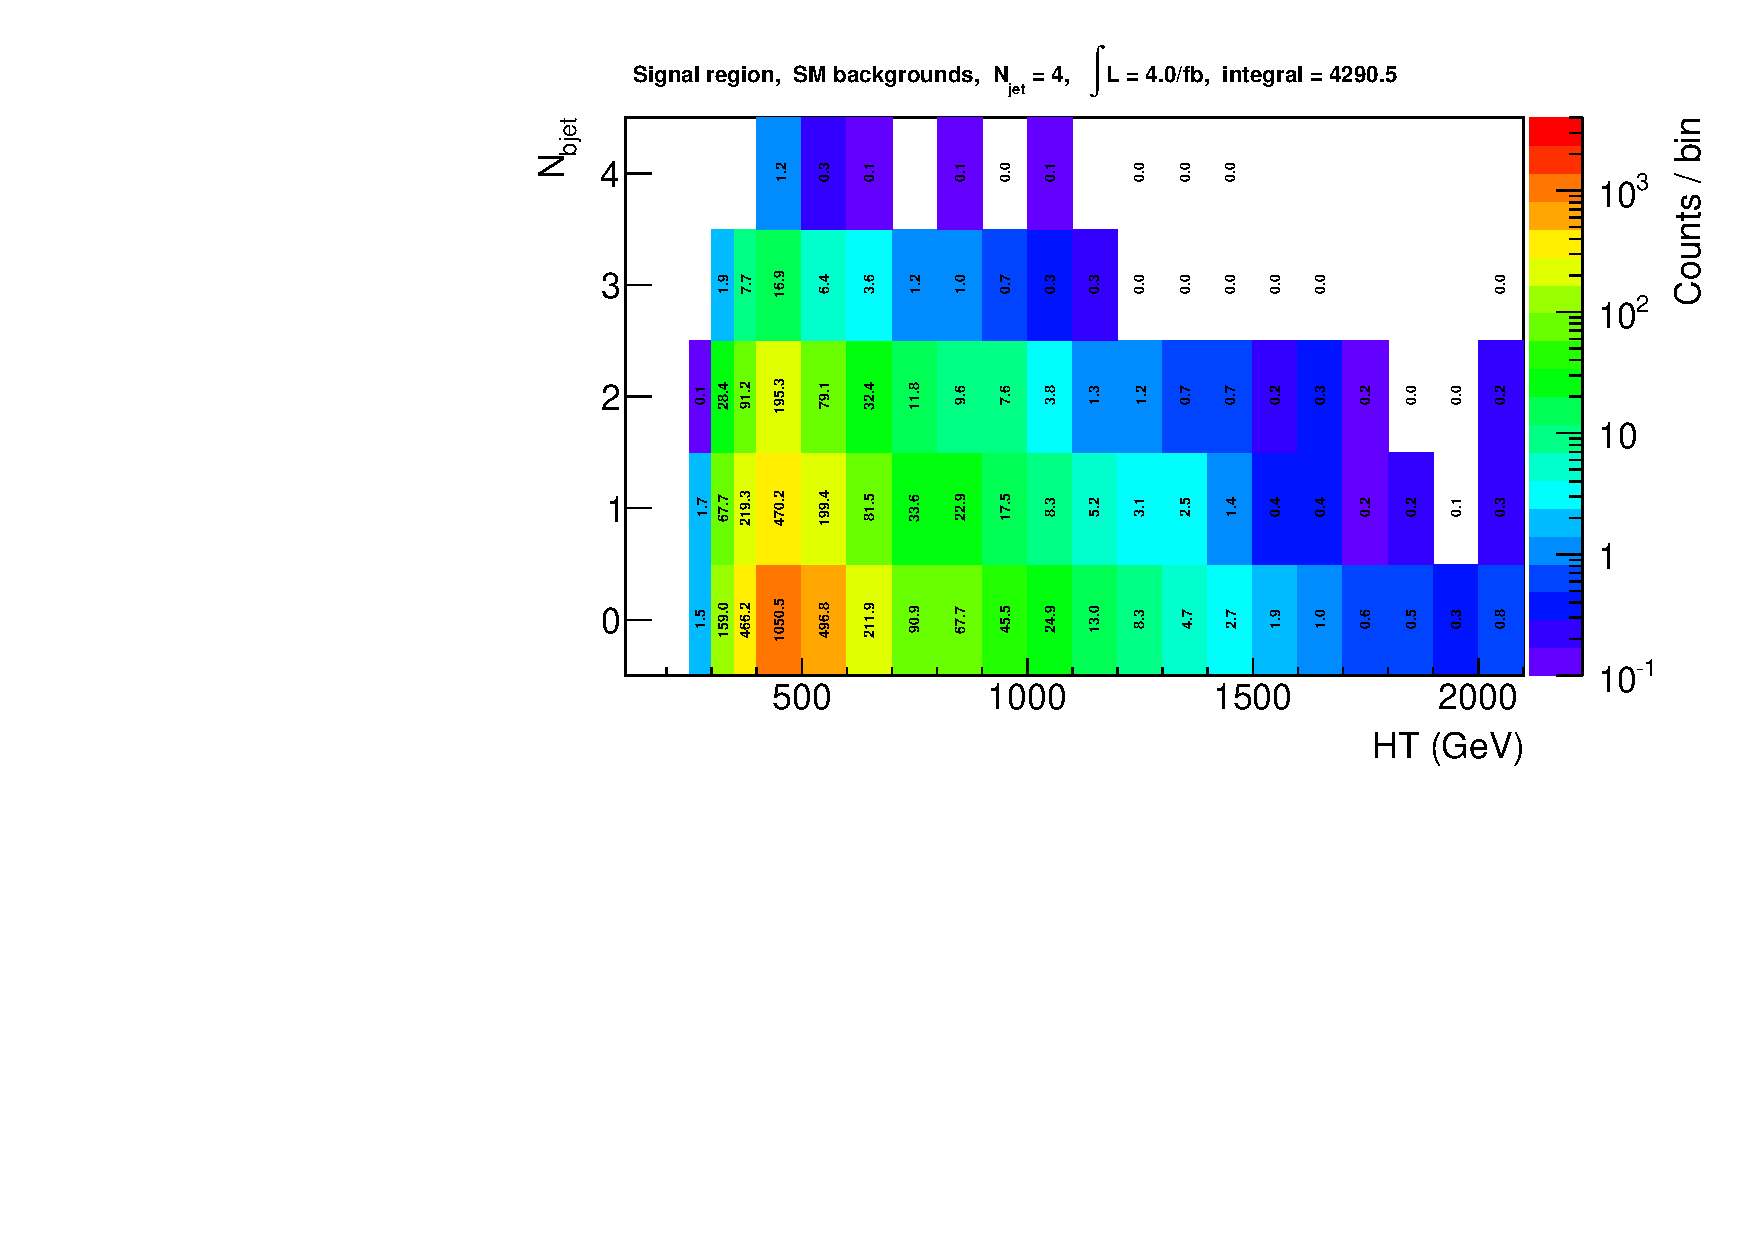
\includegraphics[width=0.5\textwidth]{figures/yieldPlots/had_ewk_eq4j.pdf}
  }~~
  \subfigure[Hadronic signal region yields for the \zInv background
  ($\njet = 4$)]{
    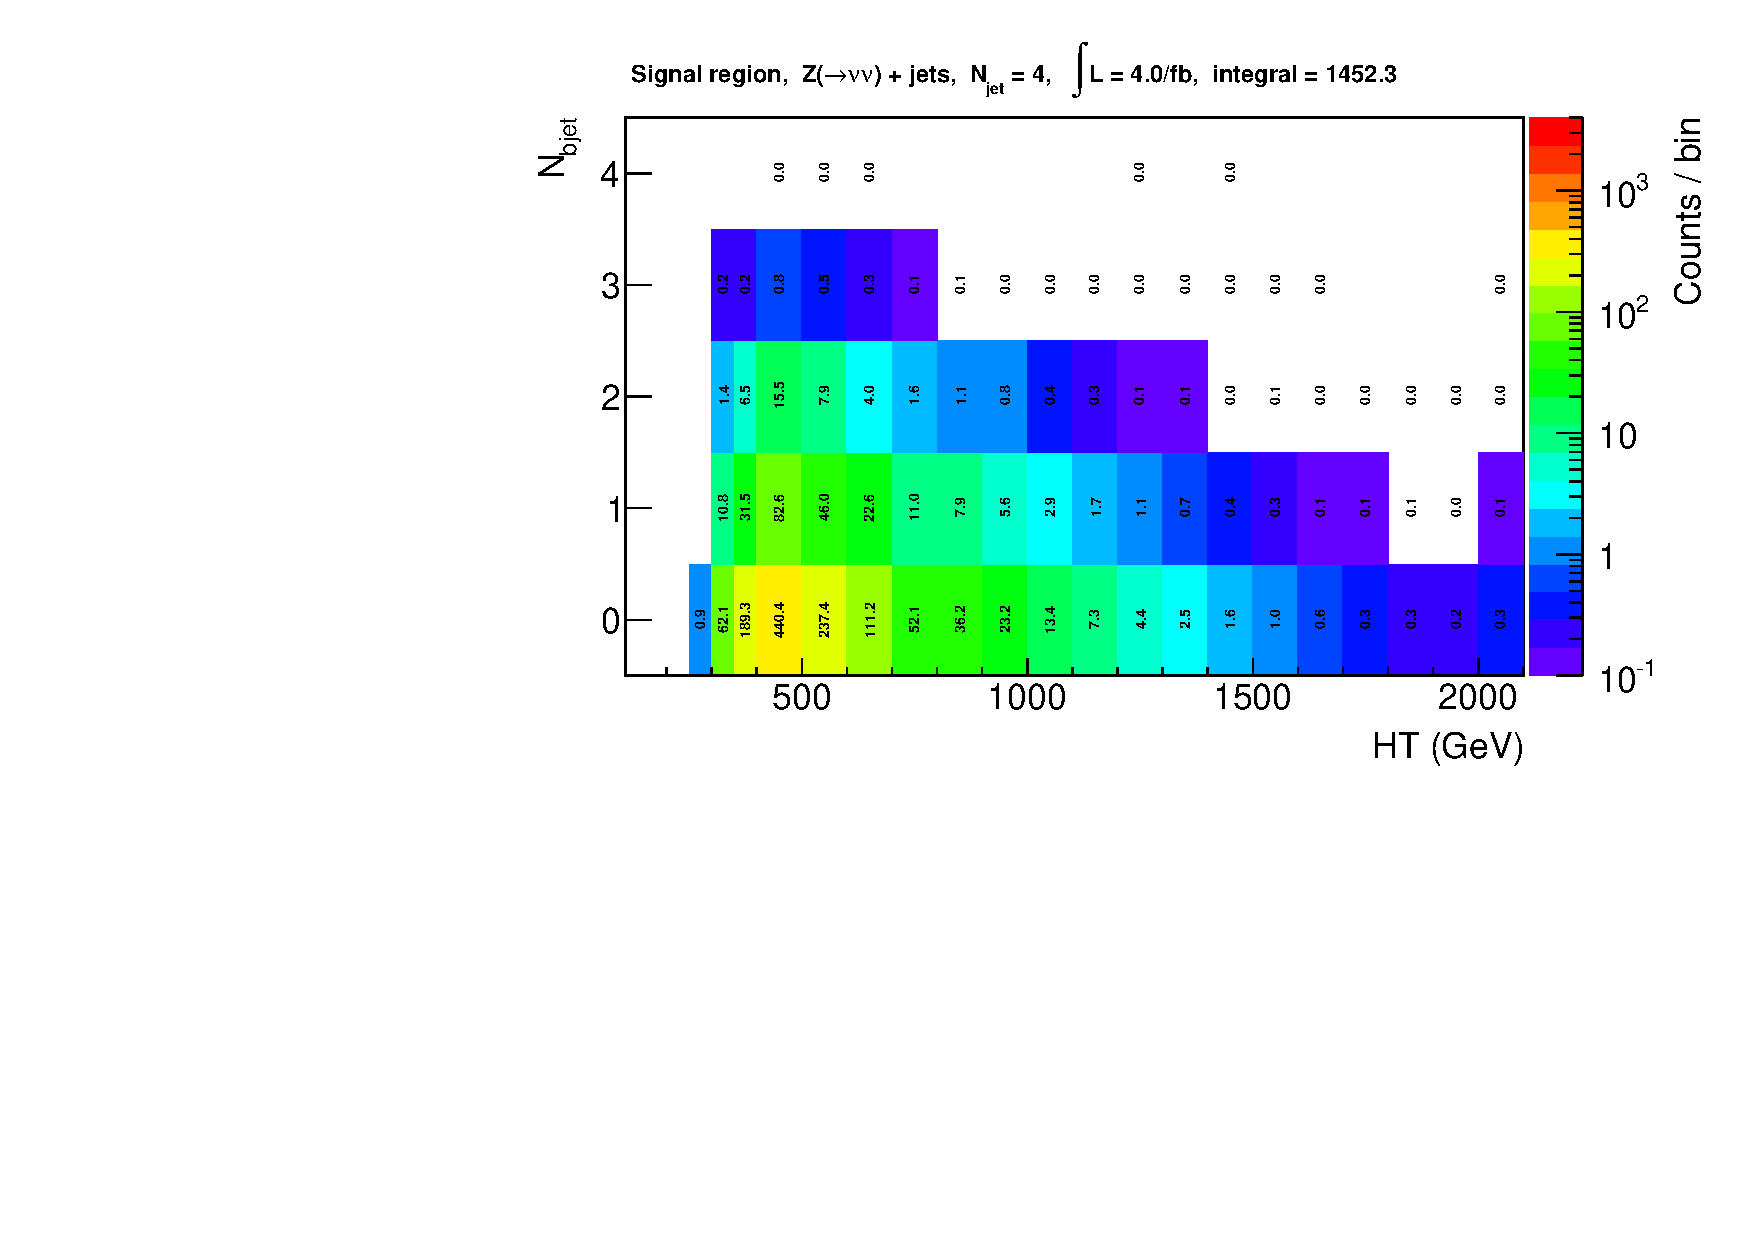
\includegraphics[width=0.5\textwidth]{figures/yieldPlots/had_zinv_eq4j.pdf}
  }\\
  \subfigure[Hadronic signal region yields for W~+~jets background
  ($\njet = 4$)]{
    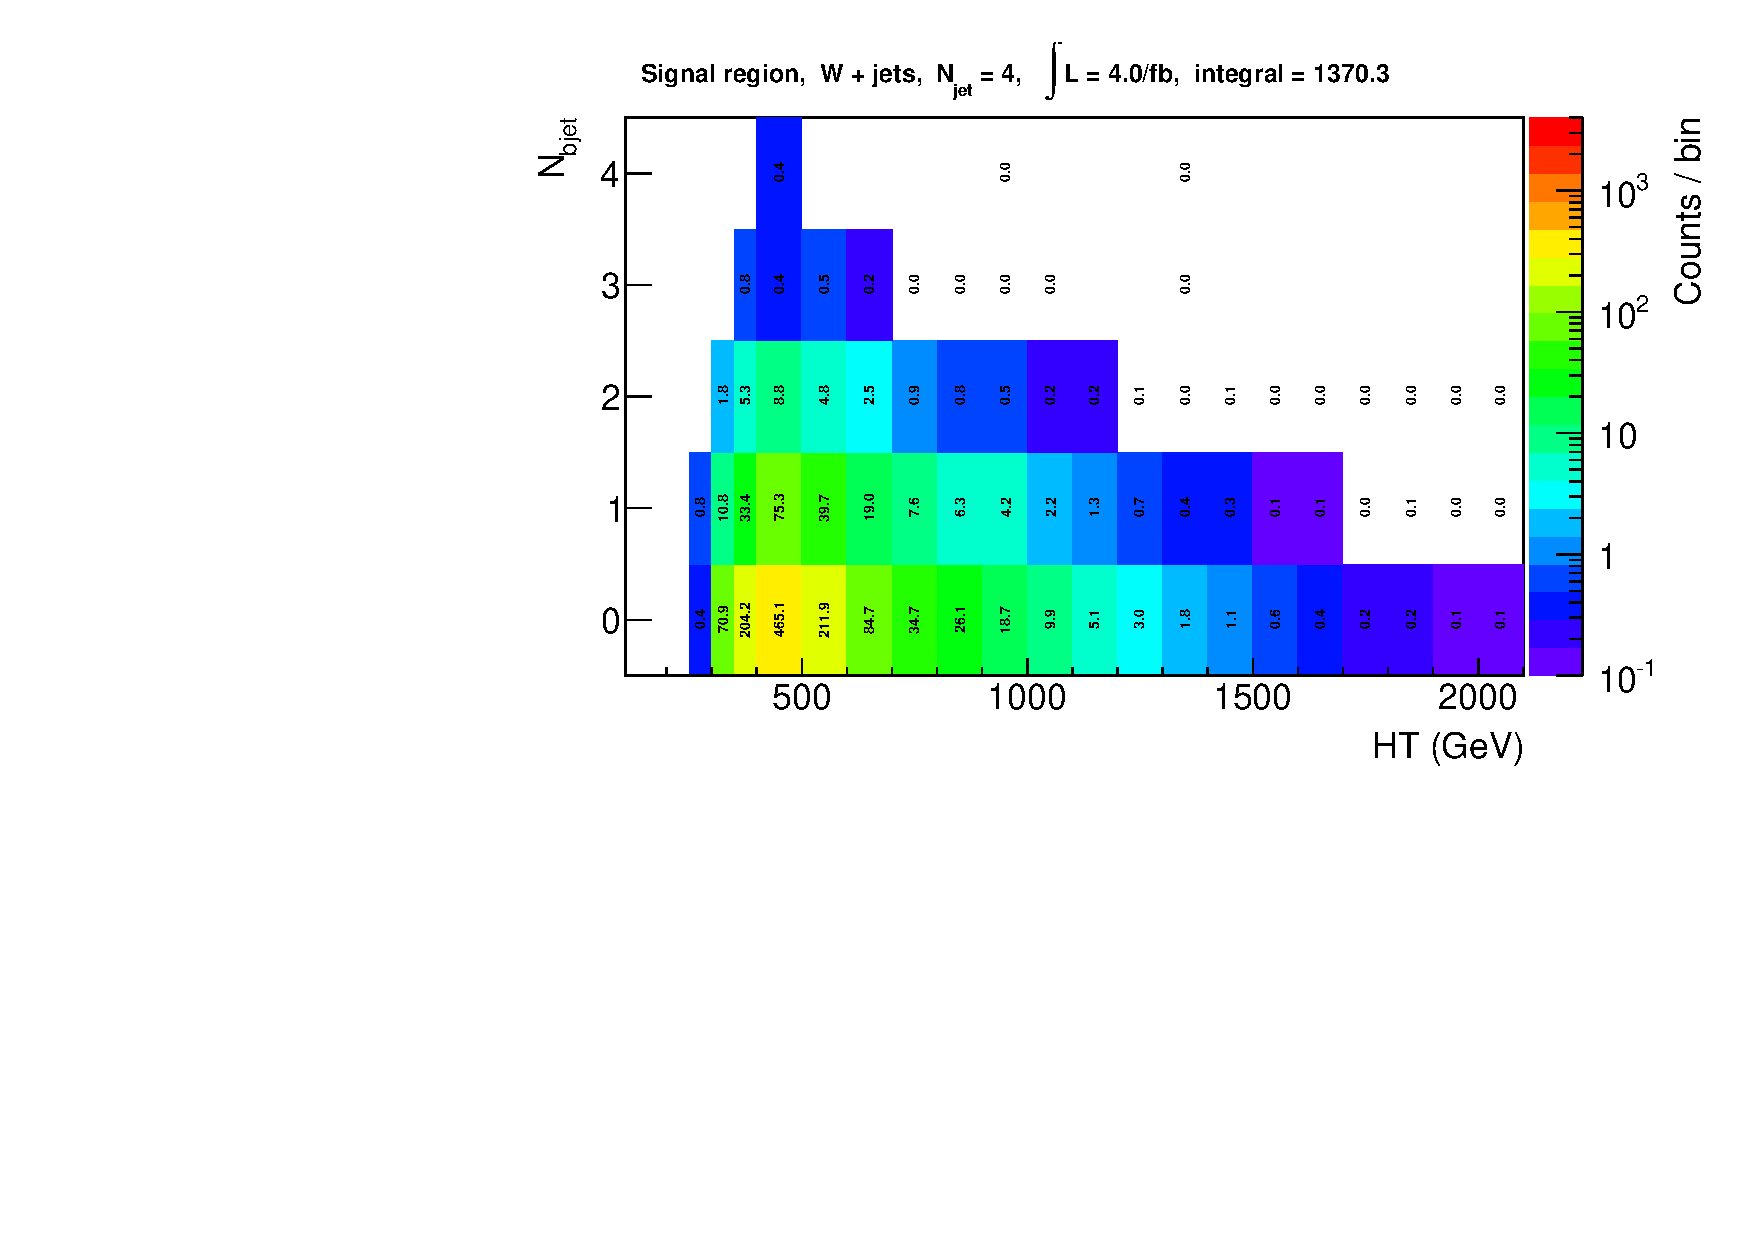
\includegraphics[width=0.5\textwidth]{figures/yieldPlots/had_wjets_eq4j.pdf}
  }~~
  \subfigure[Hadronic signal region yields for \ttbar background
  ($\njet = 4$)]{
    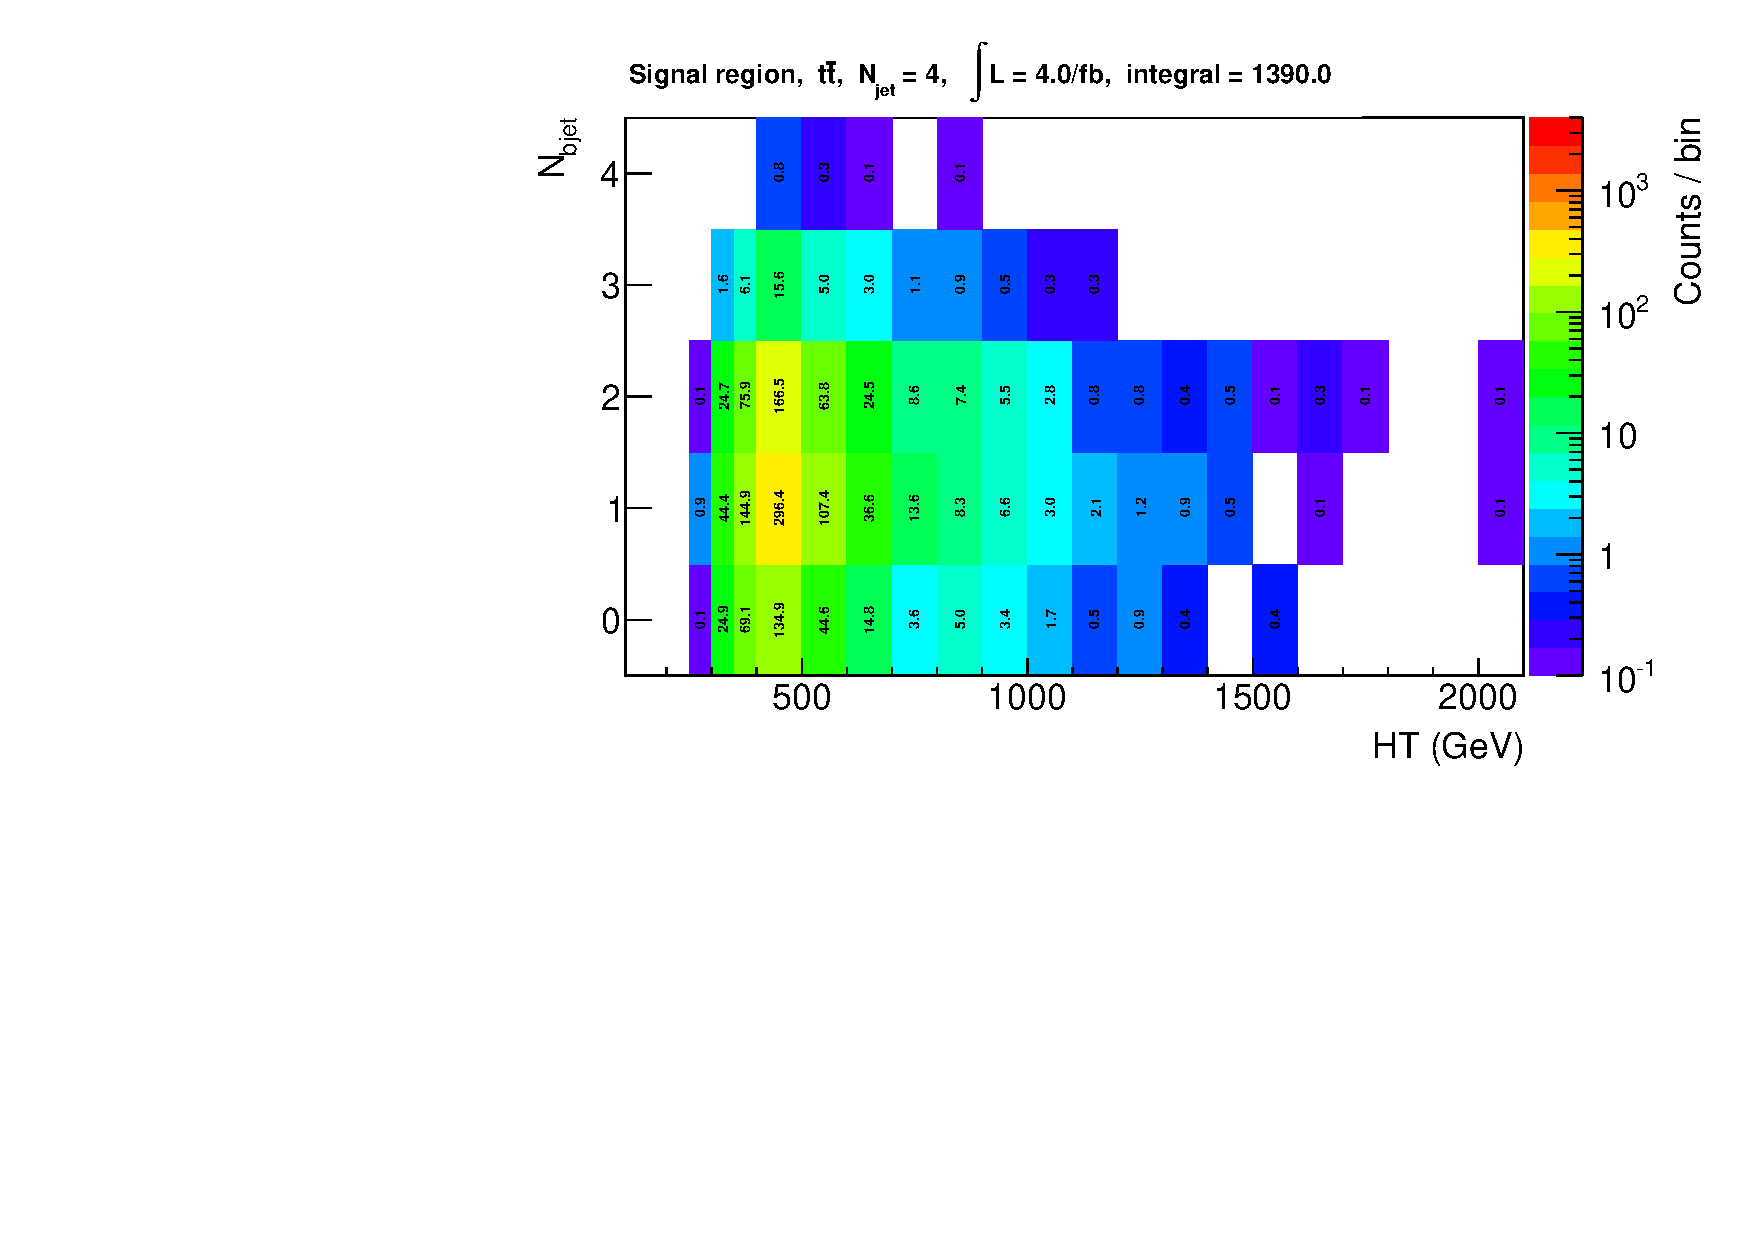
\includegraphics[width=0.5\textwidth]{figures/yieldPlots/had_ttbar_eq4j.pdf}
  }
  \caption{\label{fig:ewkYields3} Yields at $4\fbinv$ for the electroweak backgrounds in the
  hadronic signal region, $\njet=4$. The binning is chosen to be in line with the analysis
  bins. The contribution from the dominant backgrounds is shown separately.}
\end{figure}
\begin{figure}[]
  \centering
  \subfigure[Hadronic signal region yields for electroweak backgrounds
  ($\njet \geq 5$)]{
    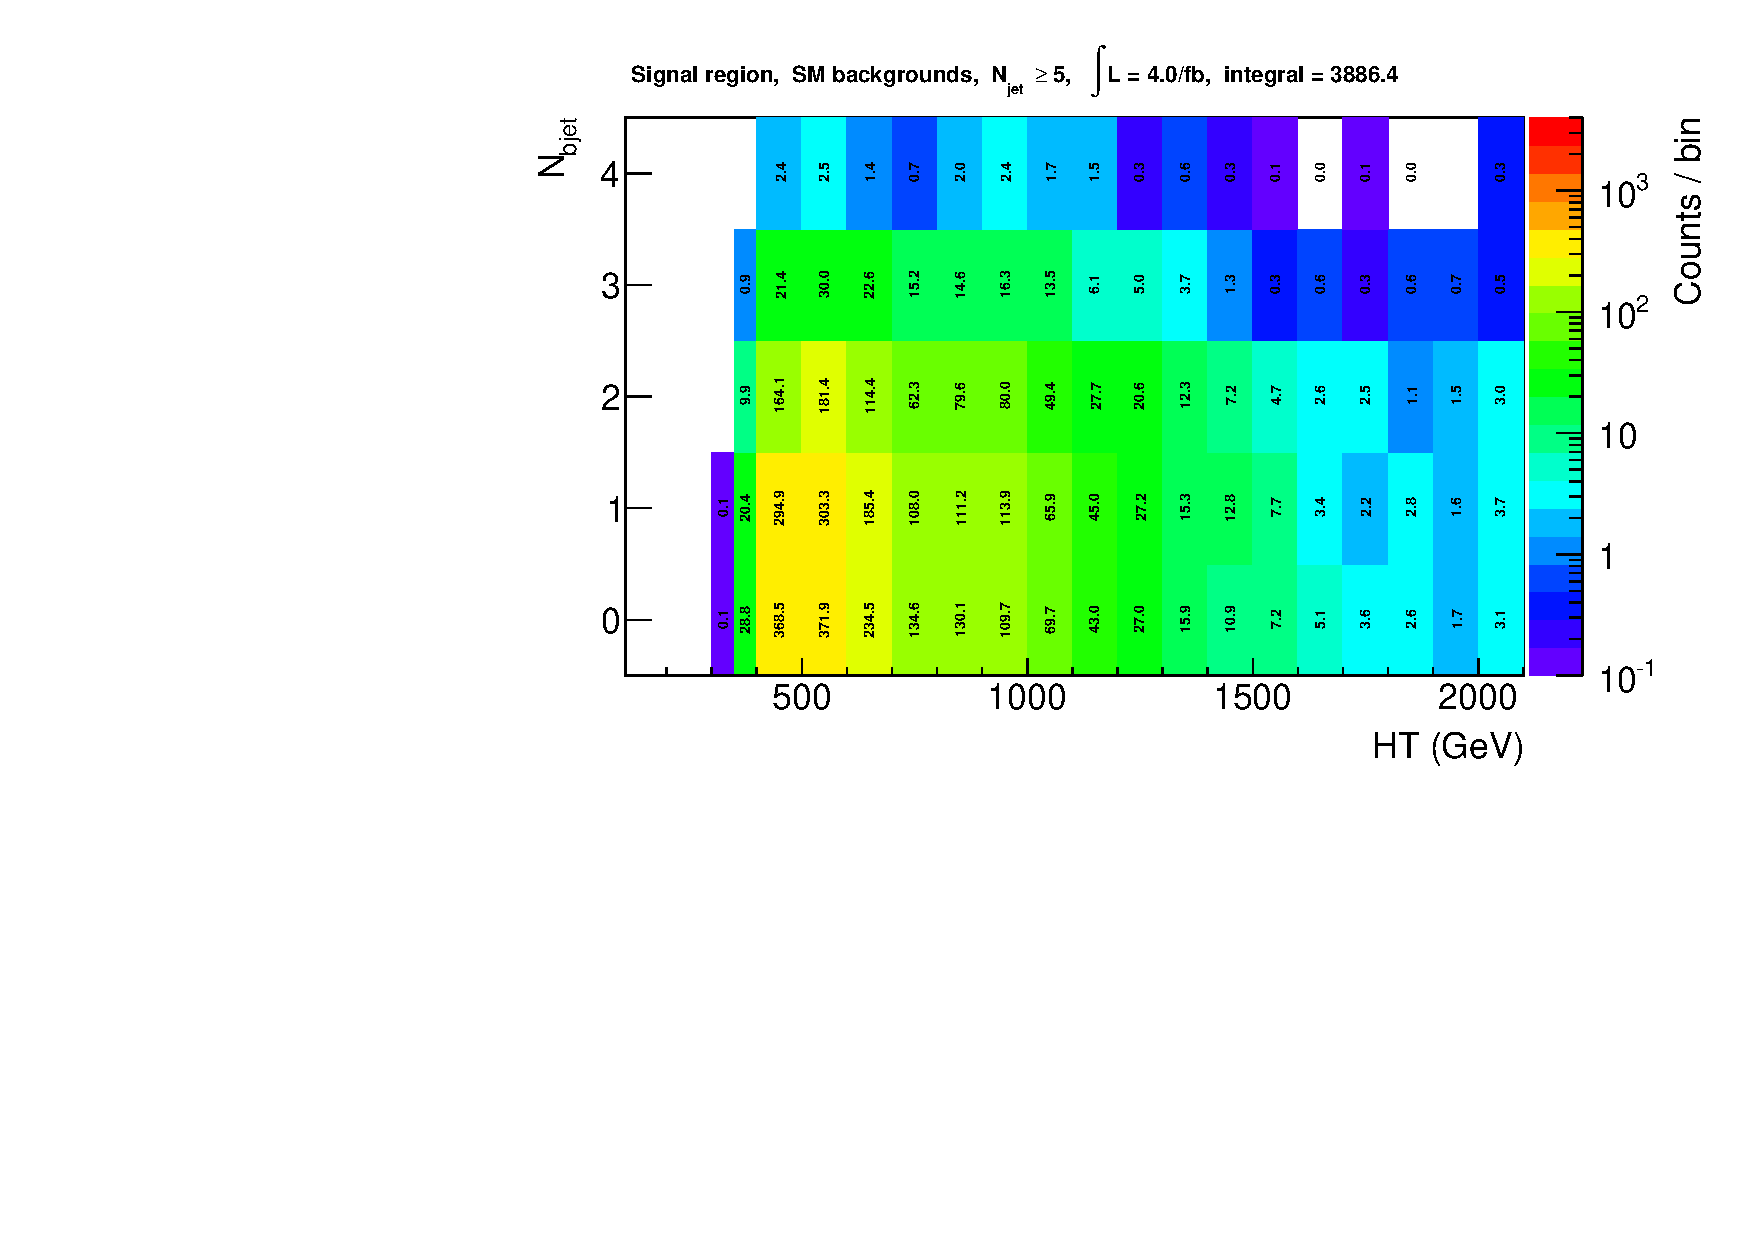
\includegraphics[width=0.5\textwidth]{figures/yieldPlots/had_ewk_ge5j.pdf}
  } ~~
  \subfigure[Hadronic signal region yields for the \zInv background
  ($\njet \geq 5$)]{
    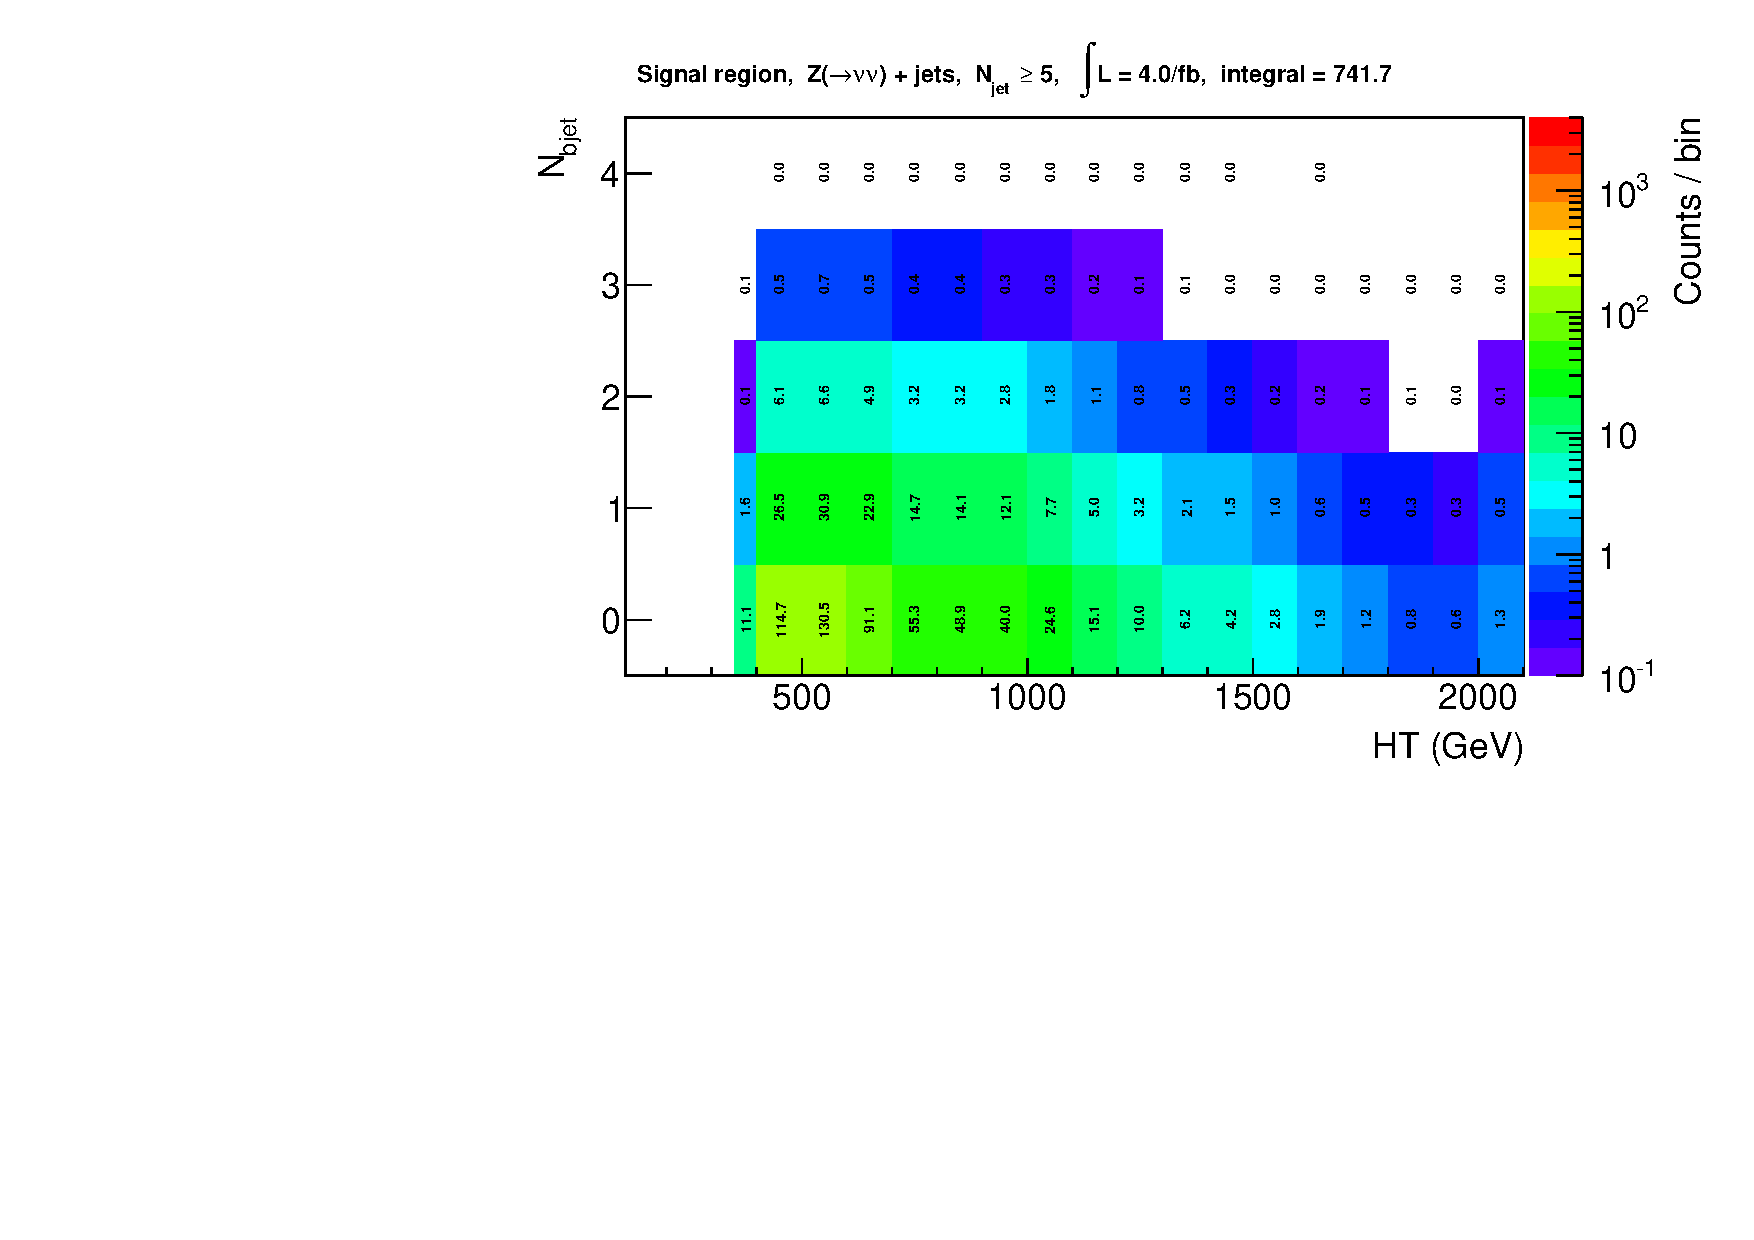
\includegraphics[width=0.5\textwidth]{figures/yieldPlots/had_zinv_ge5j.pdf}
  }\\
  \subfigure[Hadronic signal region yields for W~+~jets background
  ($\njet \geq 5$)]{
    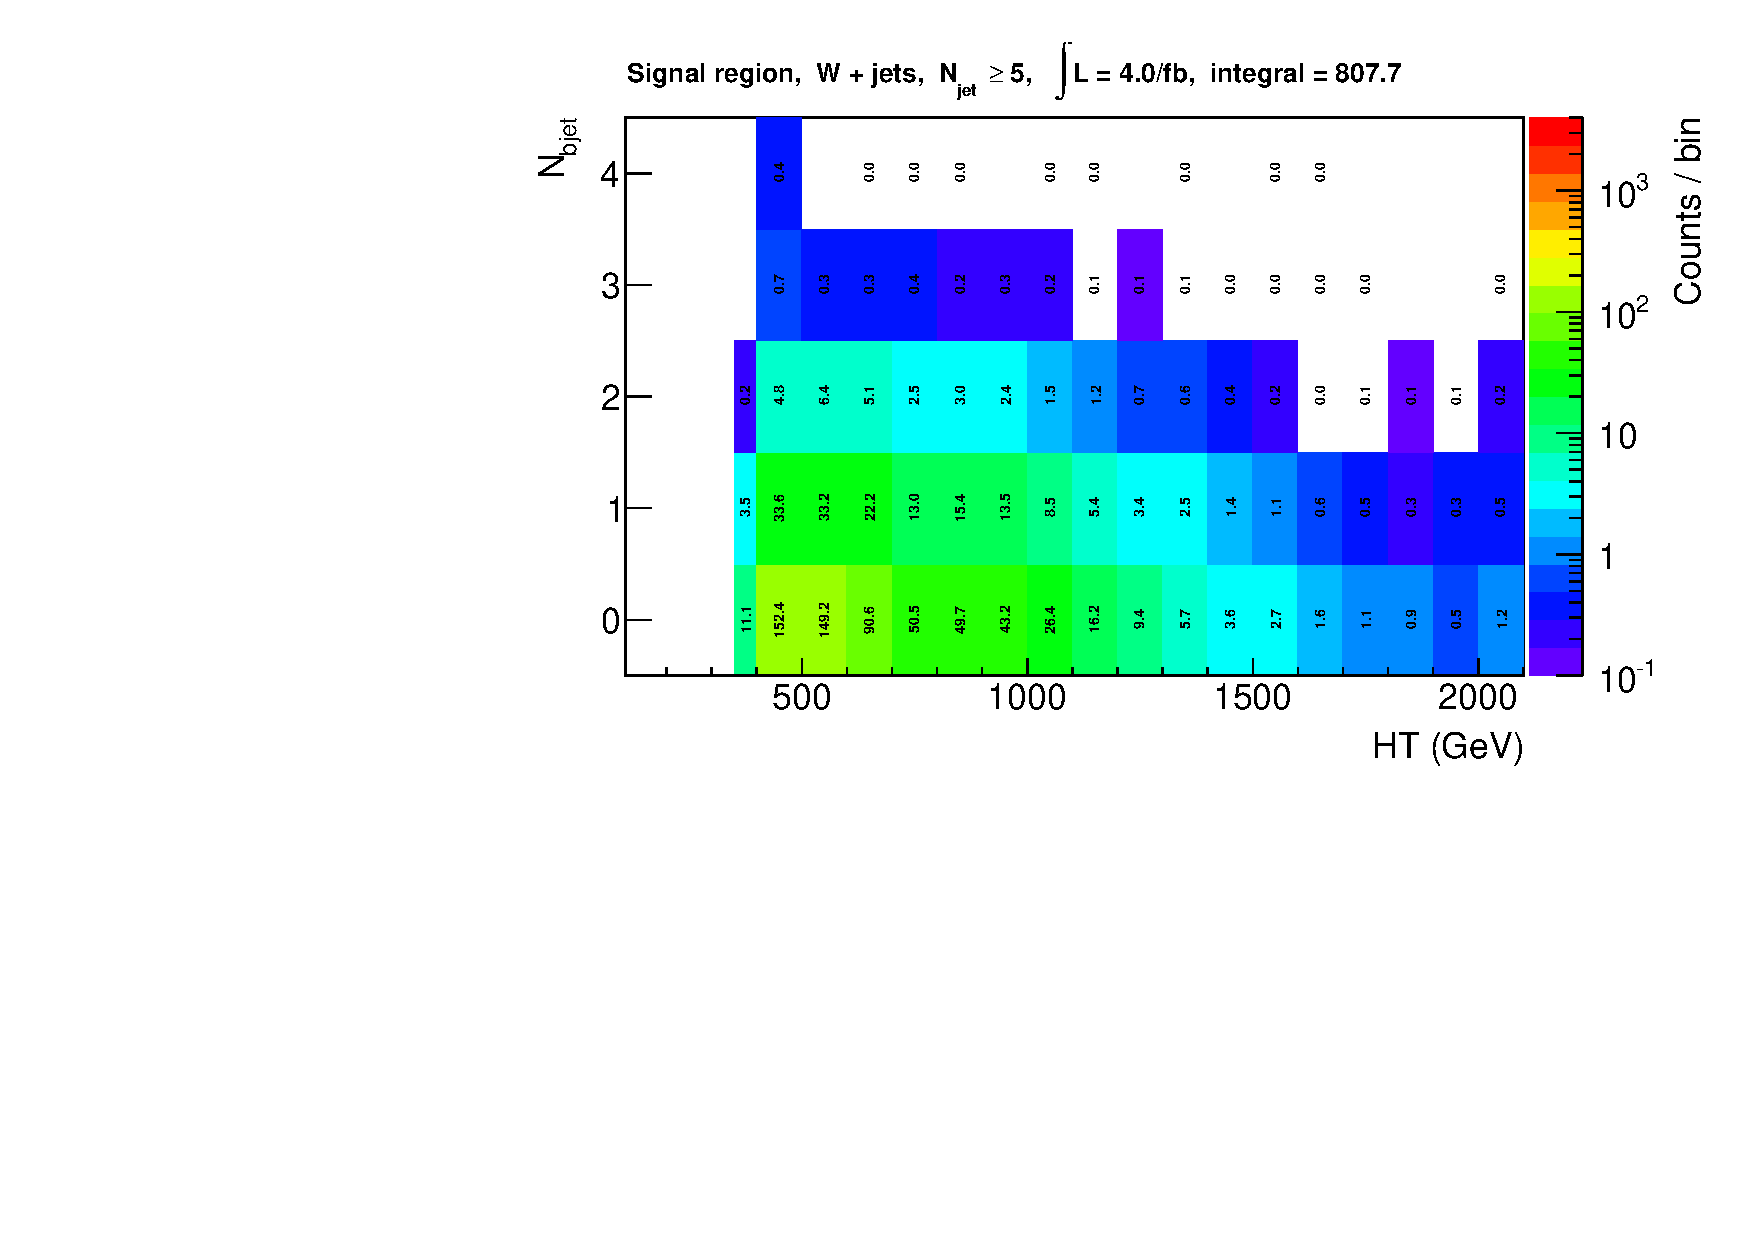
\includegraphics[width=0.5\textwidth]{figures/yieldPlots/had_wjets_ge5j.pdf}
  }~~
  \subfigure[Hadronic signal region yields for \ttbar background
  ($\njet \geq 5$)]{
    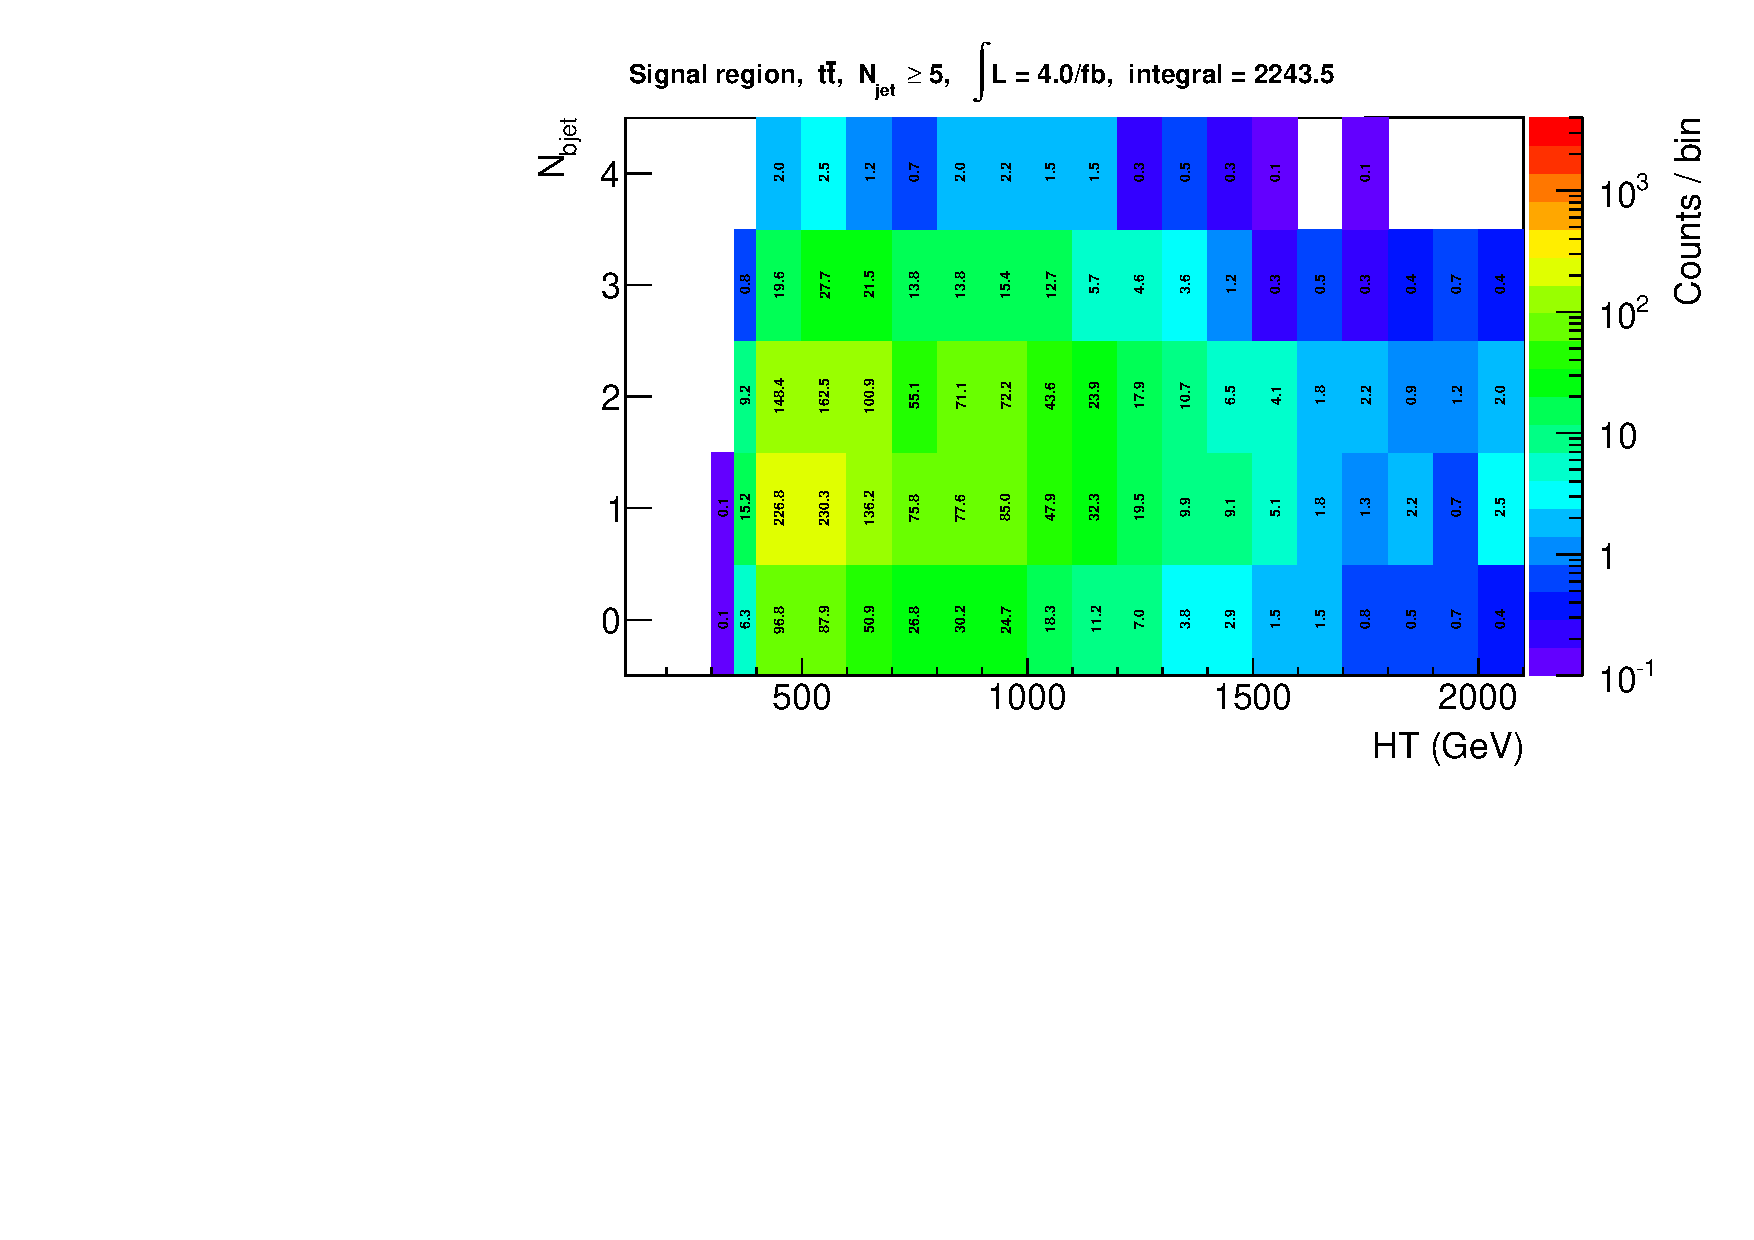
\includegraphics[width=0.5\textwidth]{figures/yieldPlots/had_ttbar_ge5j.pdf}
  }

  \\
  \subfigure[Hadronic signal region yields for T1bbbb simplified model
  \label{fig:sigYields}
  ($\njet \geq 5$)]{
    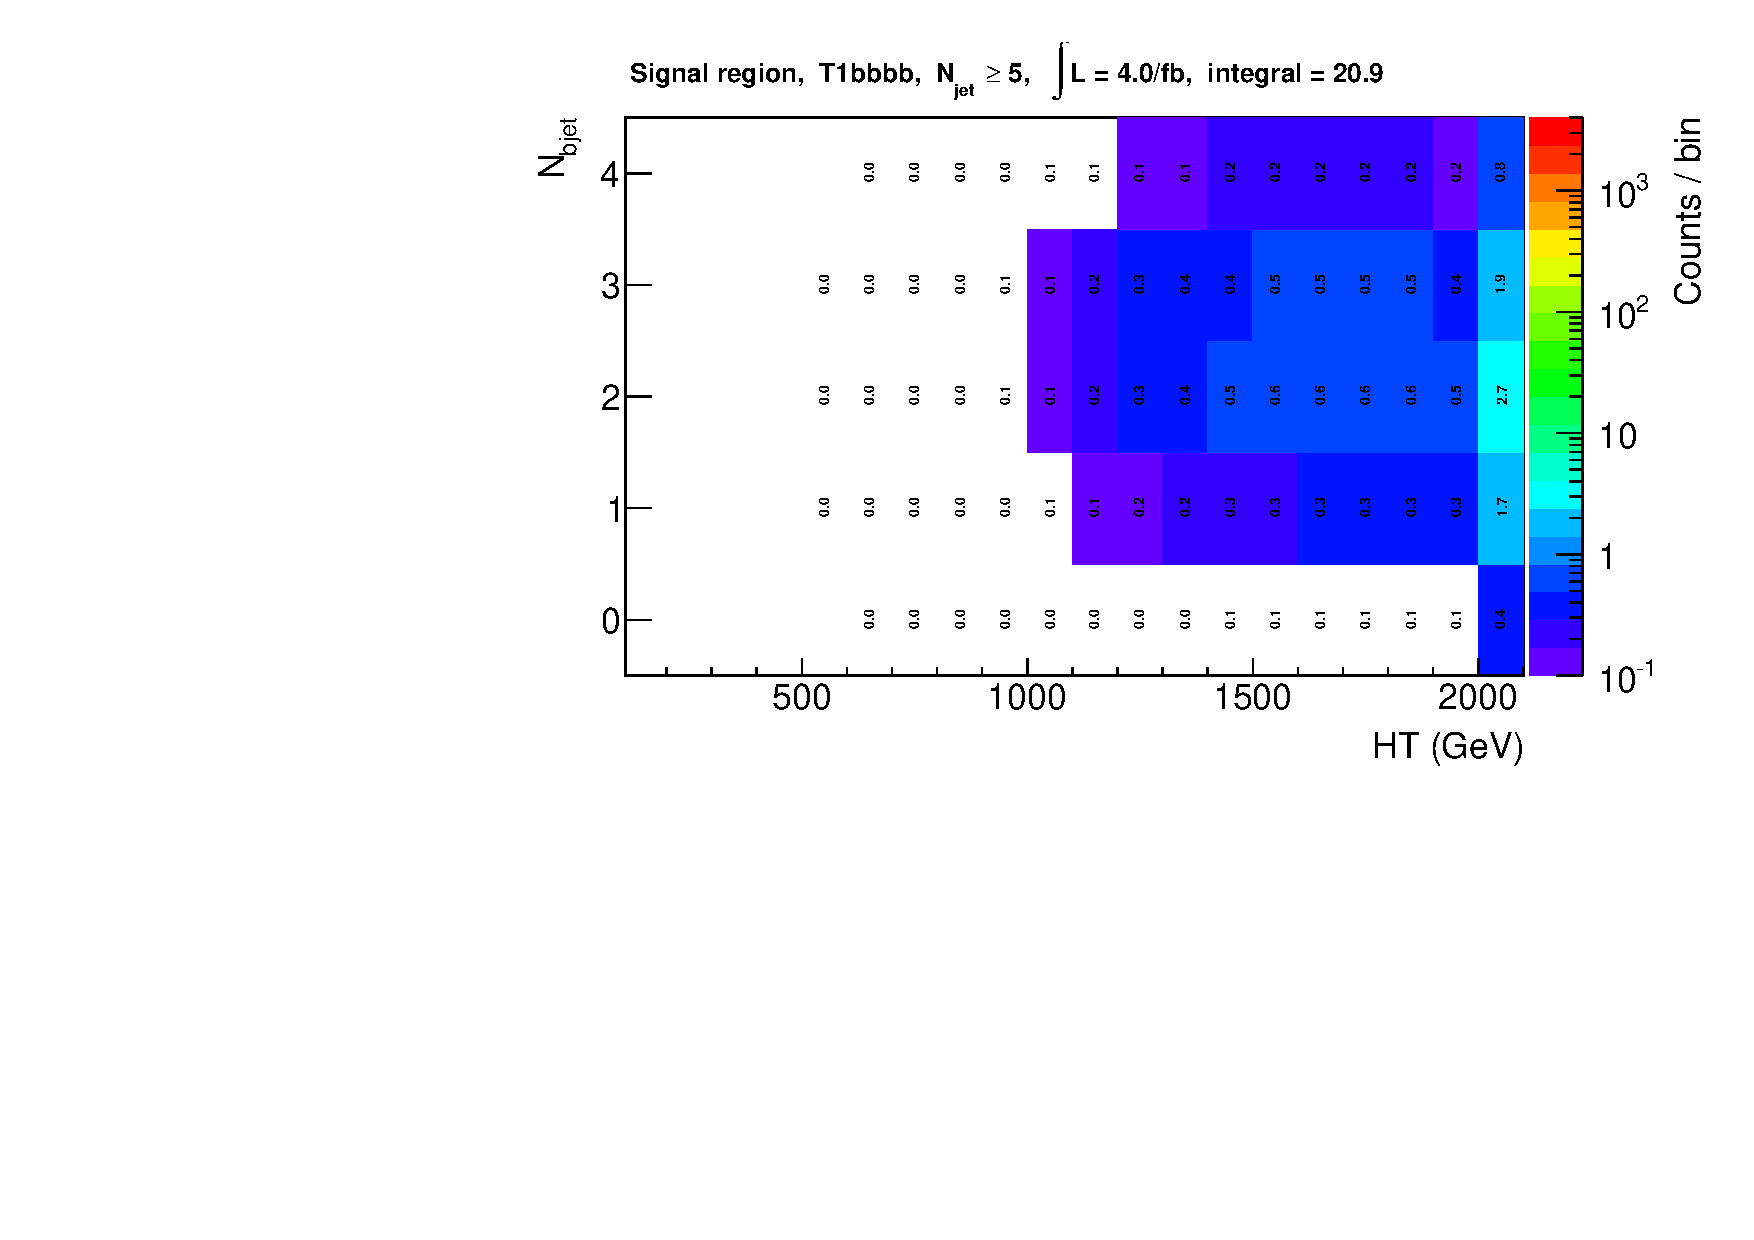
\includegraphics[width=0.5\textwidth]{figures/yieldPlots/sig_T1bbbb_ge5j.pdf}
  }
  \\
  \caption{\label{fig:ewkYields4} Yields at $4\fbinv$ for the electroweak backgrounds in the
  hadronic signal region, $\njet\geq5$. The binning is chosen to be in line with the analysis
  bins. The contribution from the dominant backgrounds is shown separately.}
\end{figure}

%%____________________________________________________________________________||
\subsection{Yields in the control samples}

The yields in the \mj, \mmj and \gj control samples can be seen in
Figures~\ref{fig:muYields}, \ref{fig:mumuYields} and \ref{fig:gammaYields}
respectively. The number of events in each of these bins is important for
working out how far we can extend in our analysis bins. We require there to be
enough events in the control samples to allow robust data driven prediction of
the backgrounds.

\begin{figure}[h!]
  \centering
  \subfigure[Yields from \texorpdfstring{\mj}{muon plus jets} control sample
  ($\njet = 2$)]{
    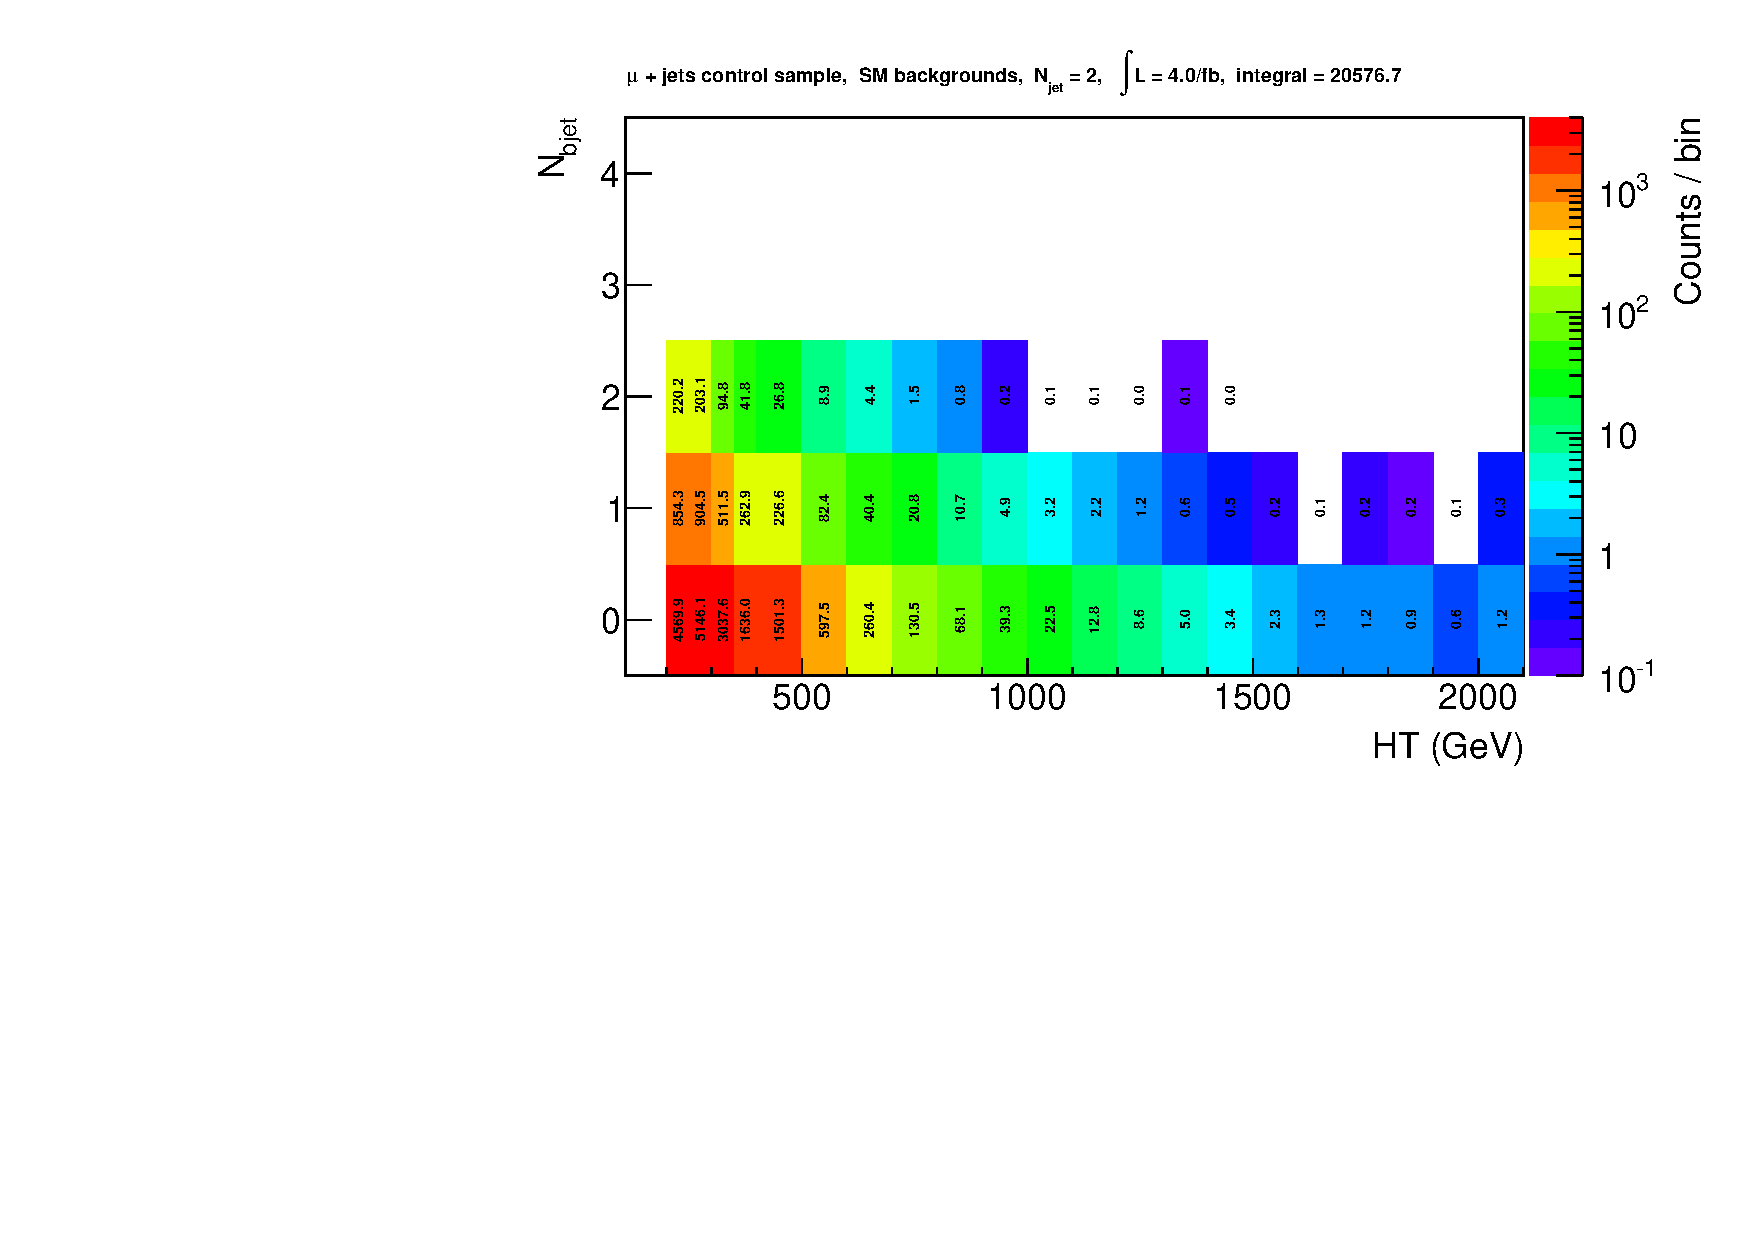
\includegraphics[width=0.5\textwidth]{figures/yieldPlots/mu_ewk_eq2j.pdf}
  }~~
  \subfigure[Yields from \texorpdfstring{\mj}{muon plus jets} control sample
  ($\njet = 3$)]{
    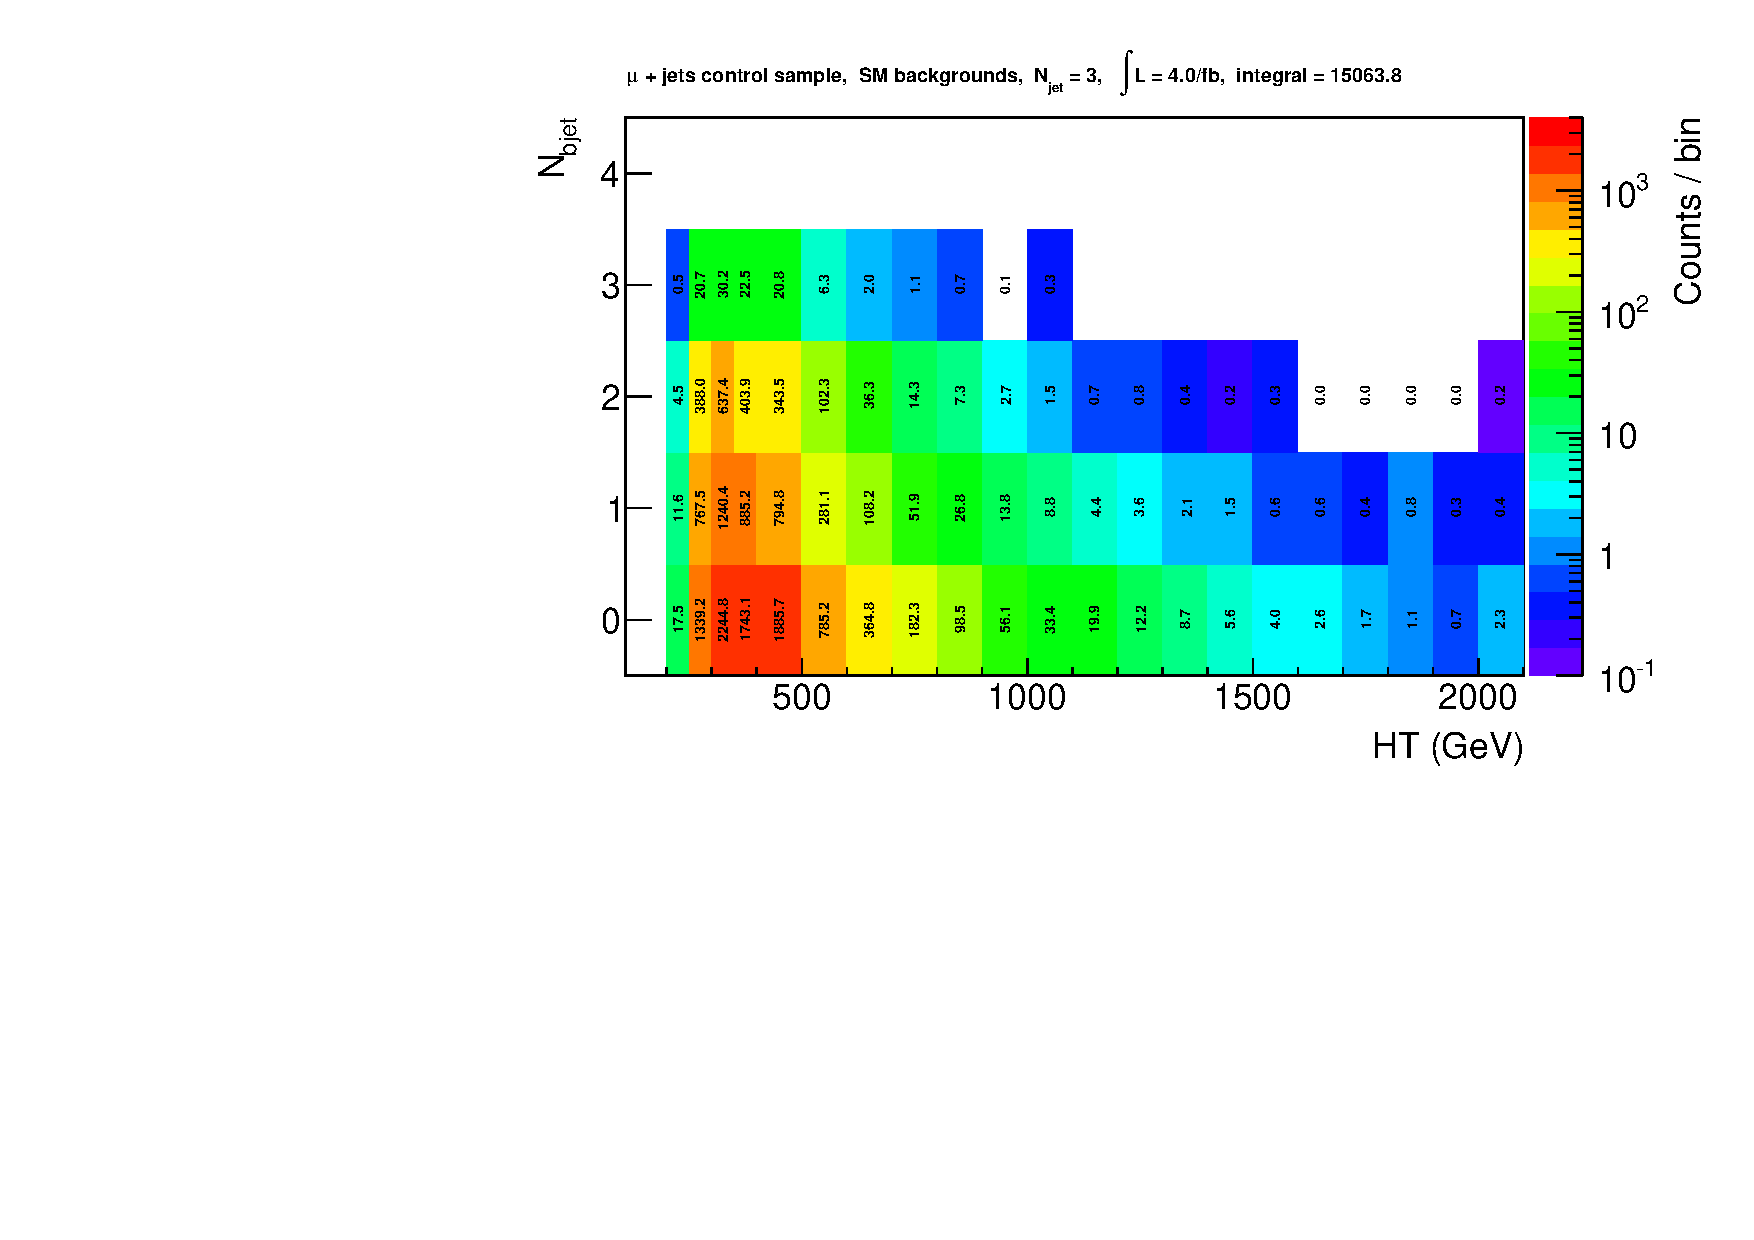
\includegraphics[width=0.5\textwidth]{figures/yieldPlots/mu_ewk_eq3j.pdf}
  }
  \\
  \subfigure[Yields from \texorpdfstring{\mj}{muon plus jets} control sample
  ($\njet = 4$)]{
    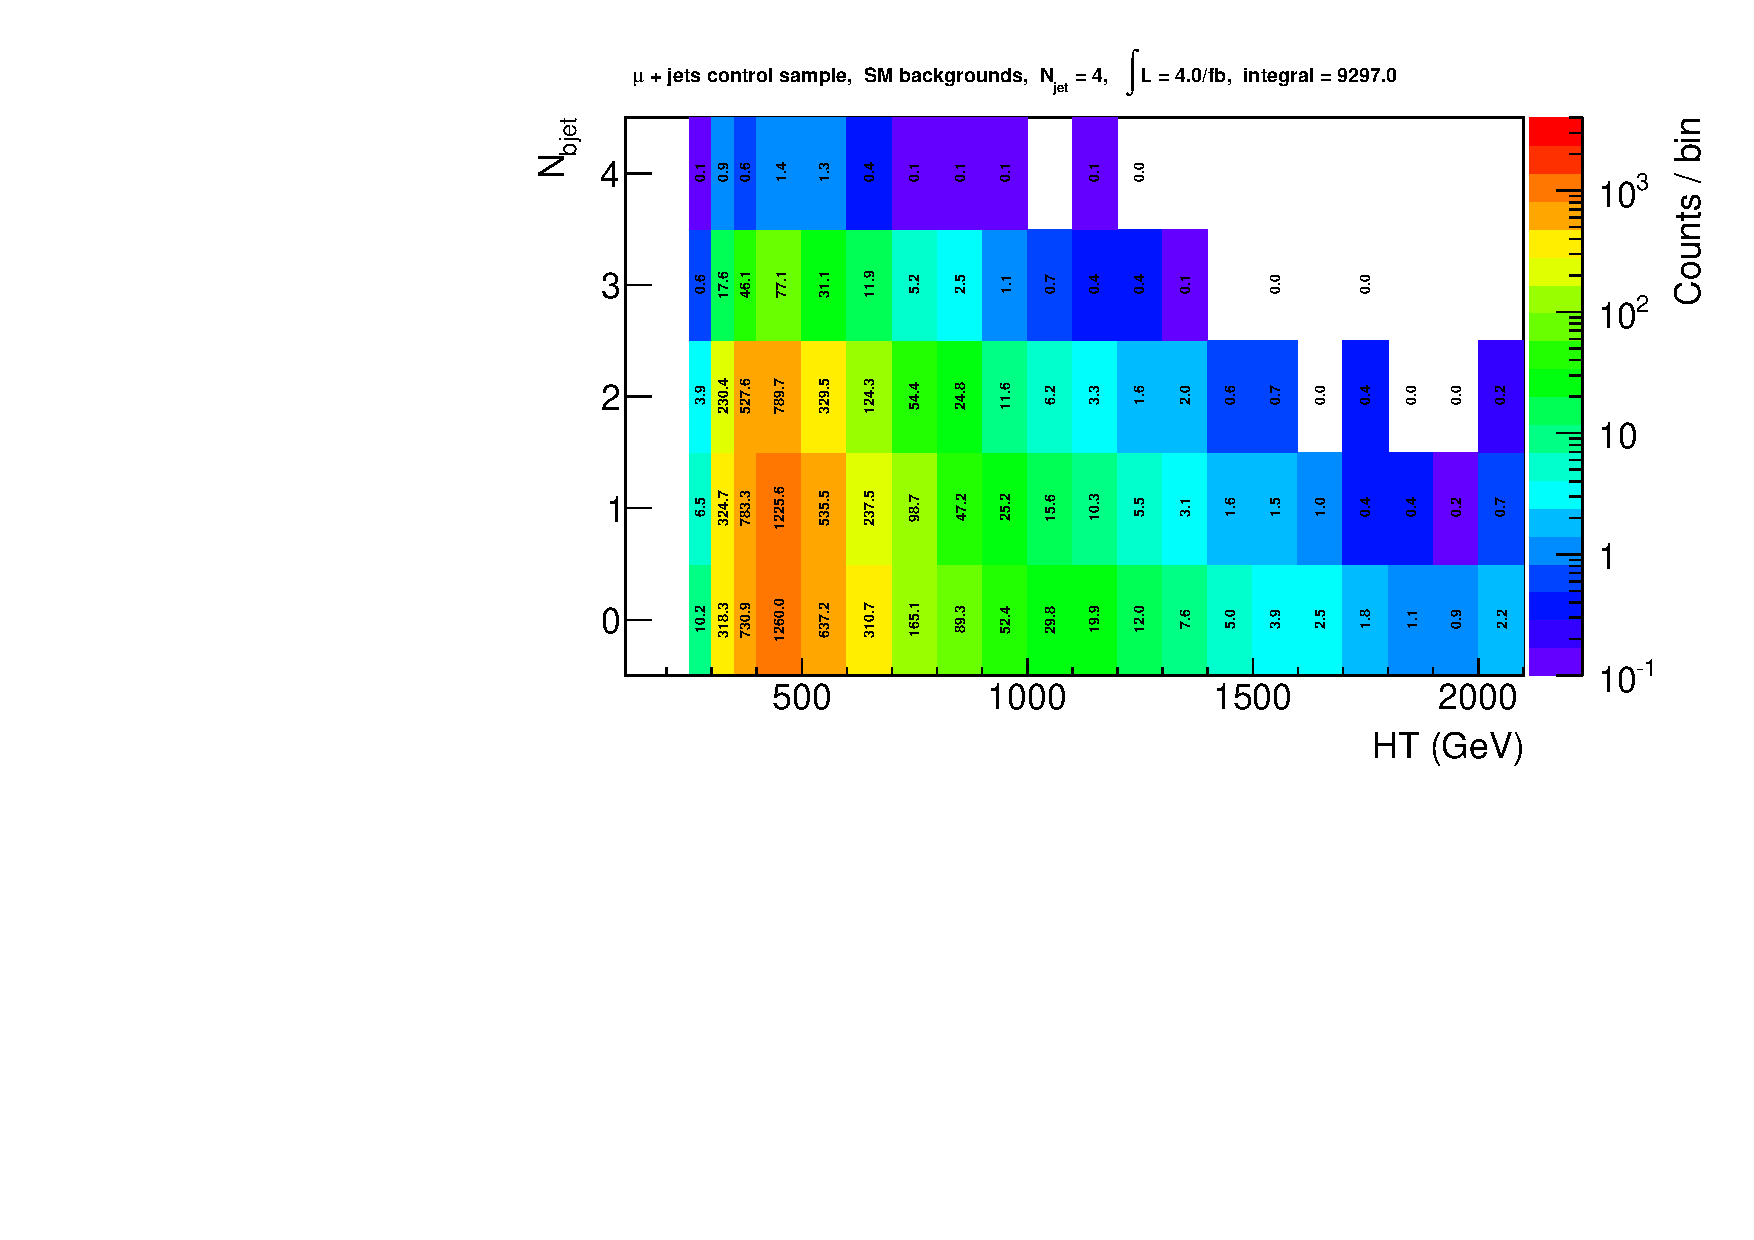
\includegraphics[width=0.5\textwidth]{figures/yieldPlots/mu_ewk_eq4j.pdf}
  }~~
  \subfigure[Yields from \texorpdfstring{\mj}{muon plus jets} control sample
  ($\njet \geq 5$)]{
    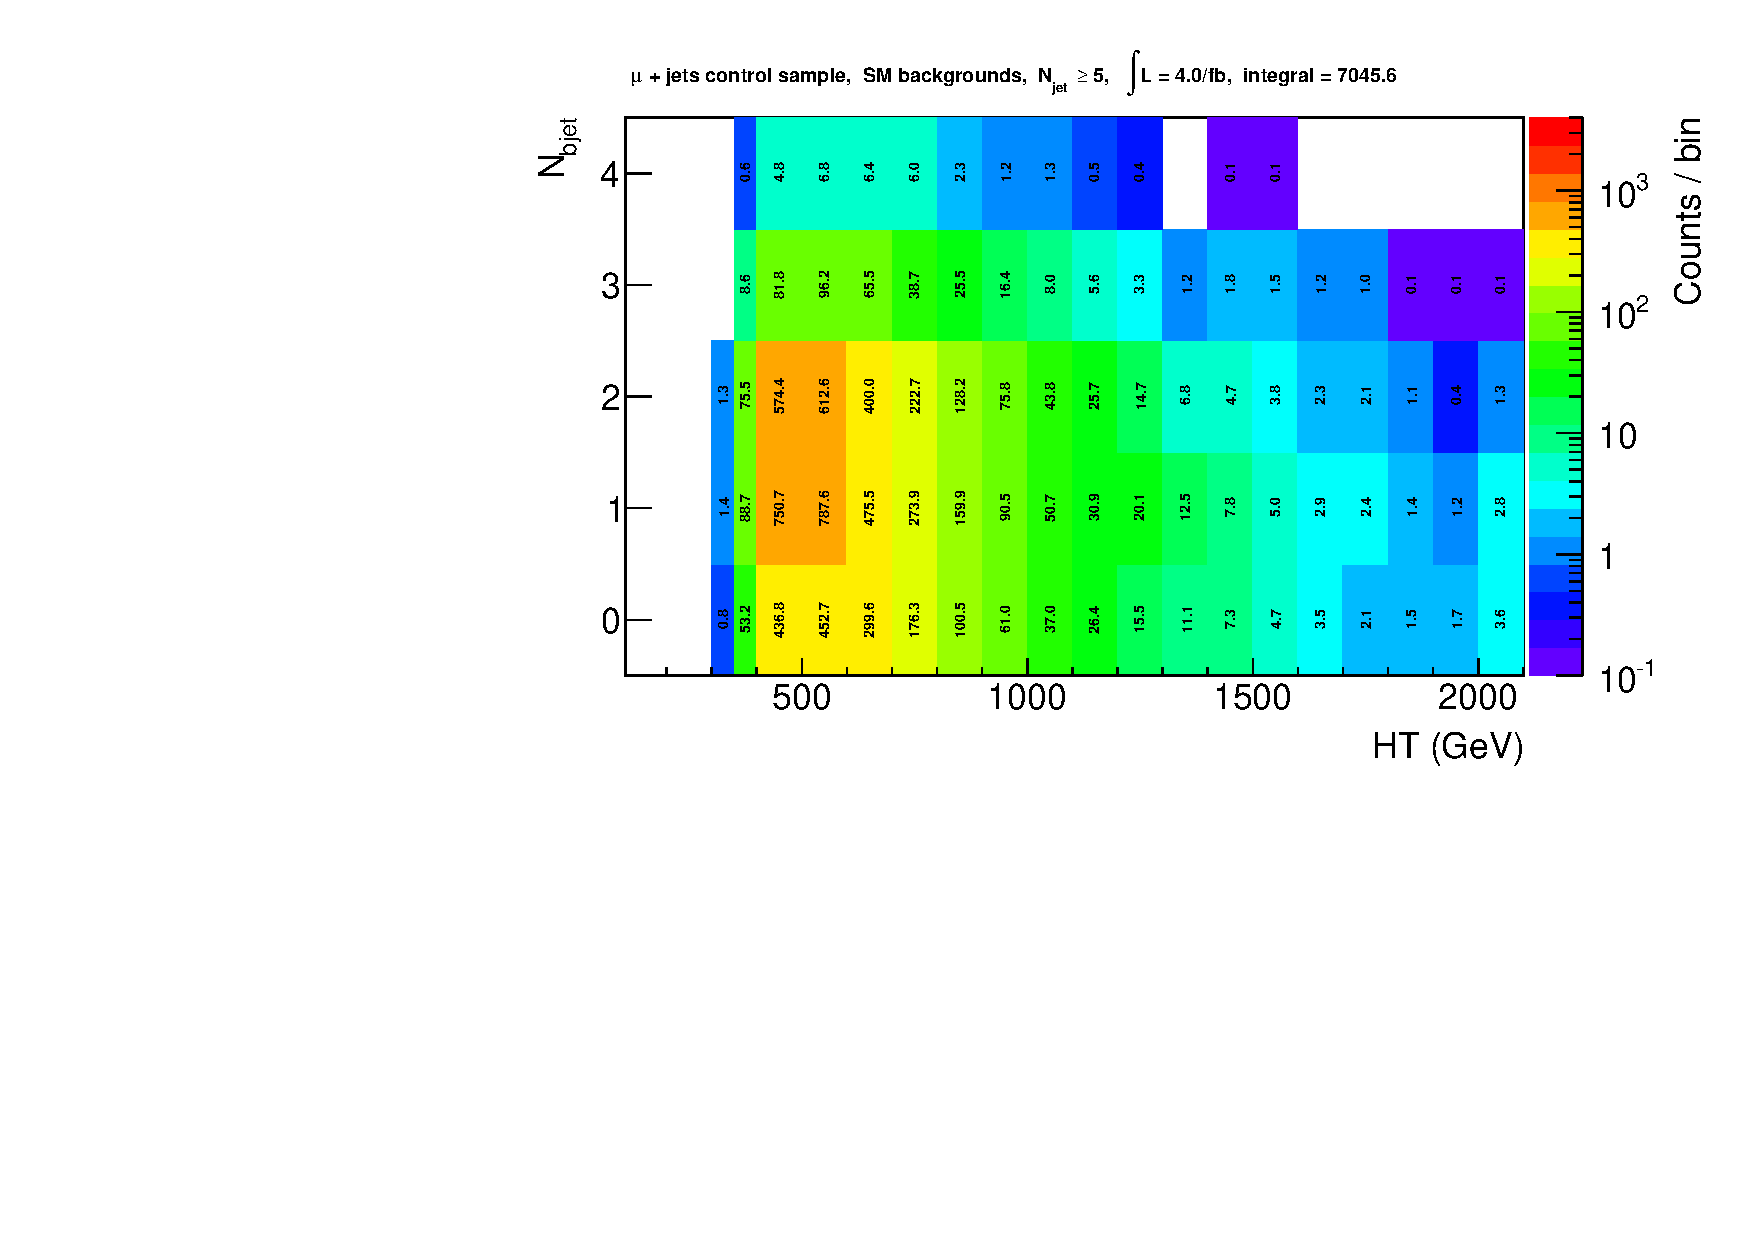
\includegraphics[width=0.5\textwidth]{figures/yieldPlots/mu_ewk_ge5j.pdf}
  } 
  \\
  \caption{\label{fig:muYields} Yields at $4\fbinv$ for the W~+~jets and \ttbar
  MC contributions to the \texorpdfstring{\mj}{muon plus jets} control sample. }
\end{figure}

\begin{figure}[h!]
  \centering
  \subfigure[Yields from \texorpdfstring{\mmj}{di-muon plus jets} control sample
  ($\njet = 2$)]{
    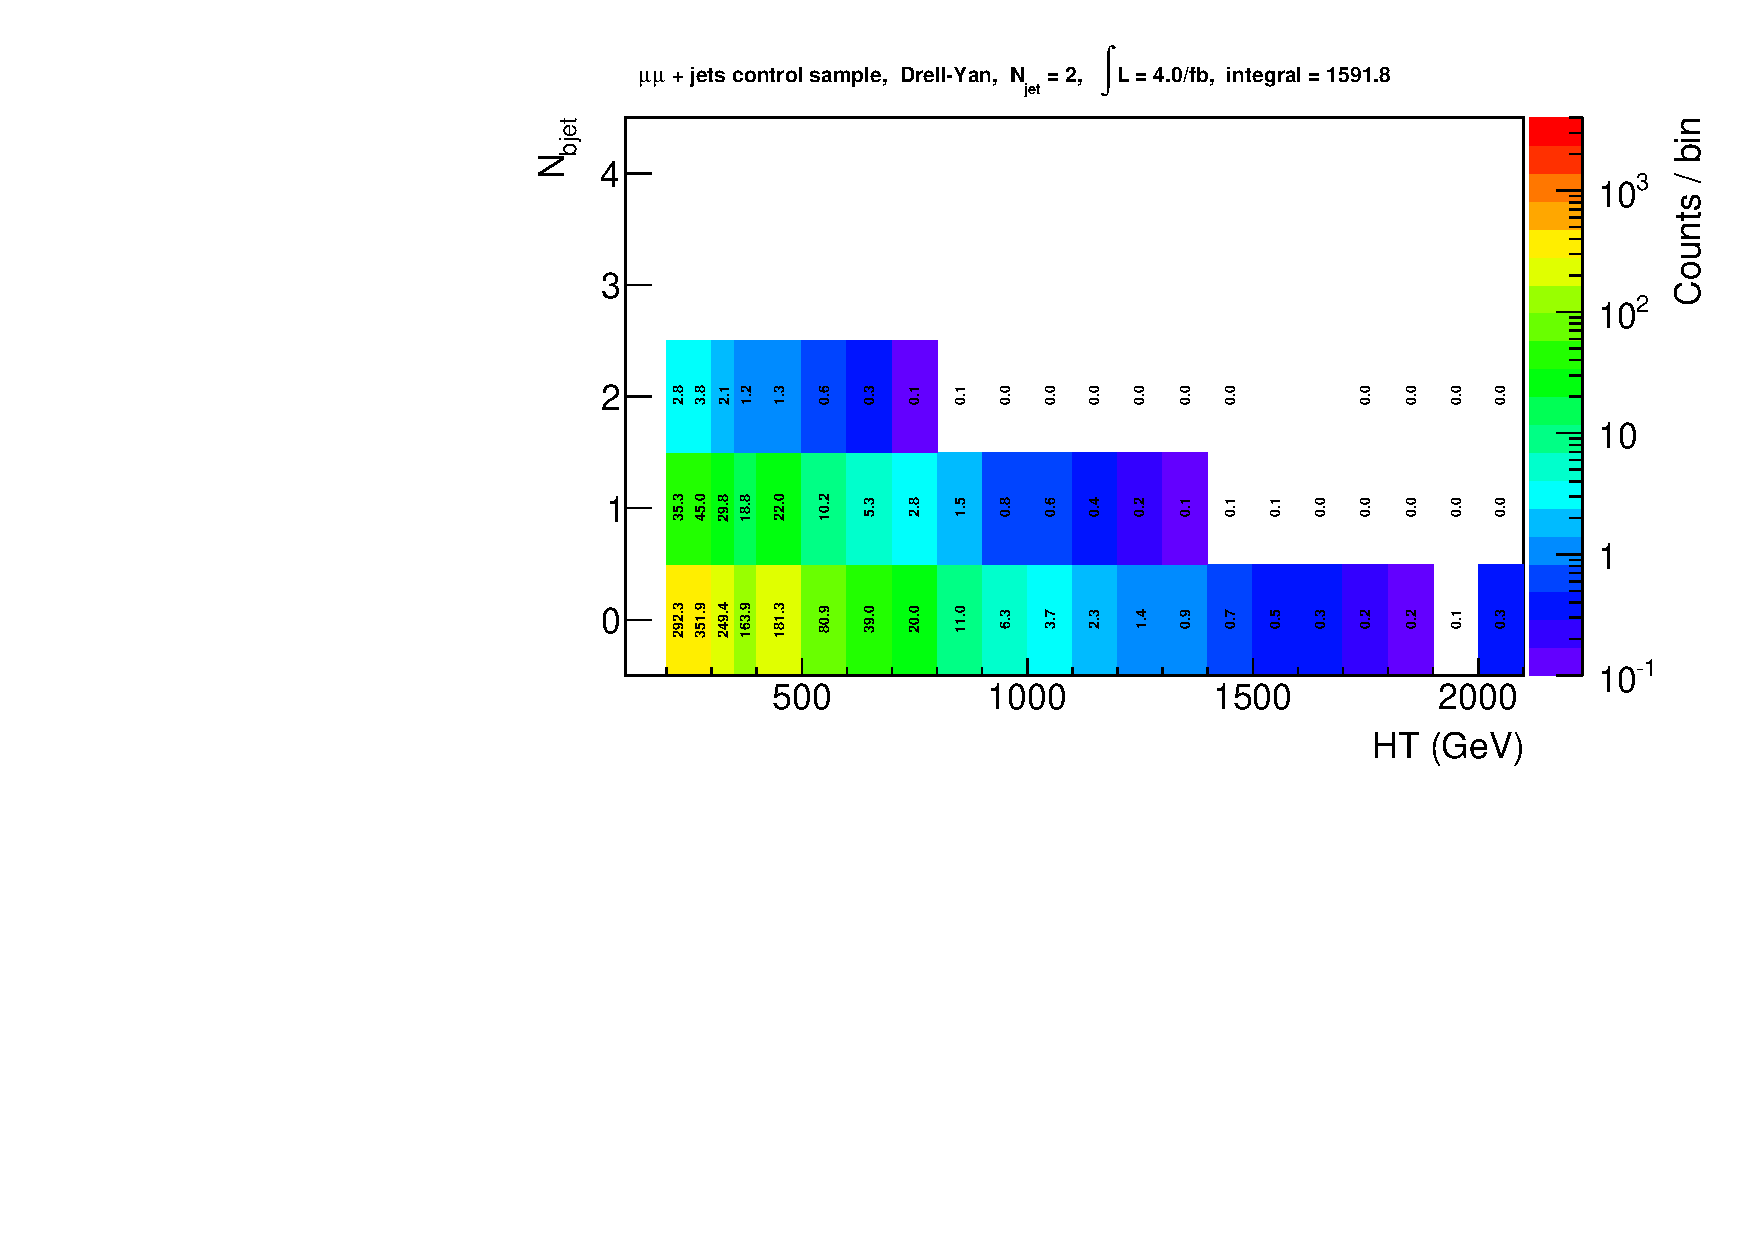
\includegraphics[width=0.5\textwidth]{figures/yieldPlots/mm_dy_eq2j.pdf}
  }~~
  \subfigure[Yields from \texorpdfstring{\mmj}{di-muon plus jets} control sample
  ($\njet = 3$)]{
    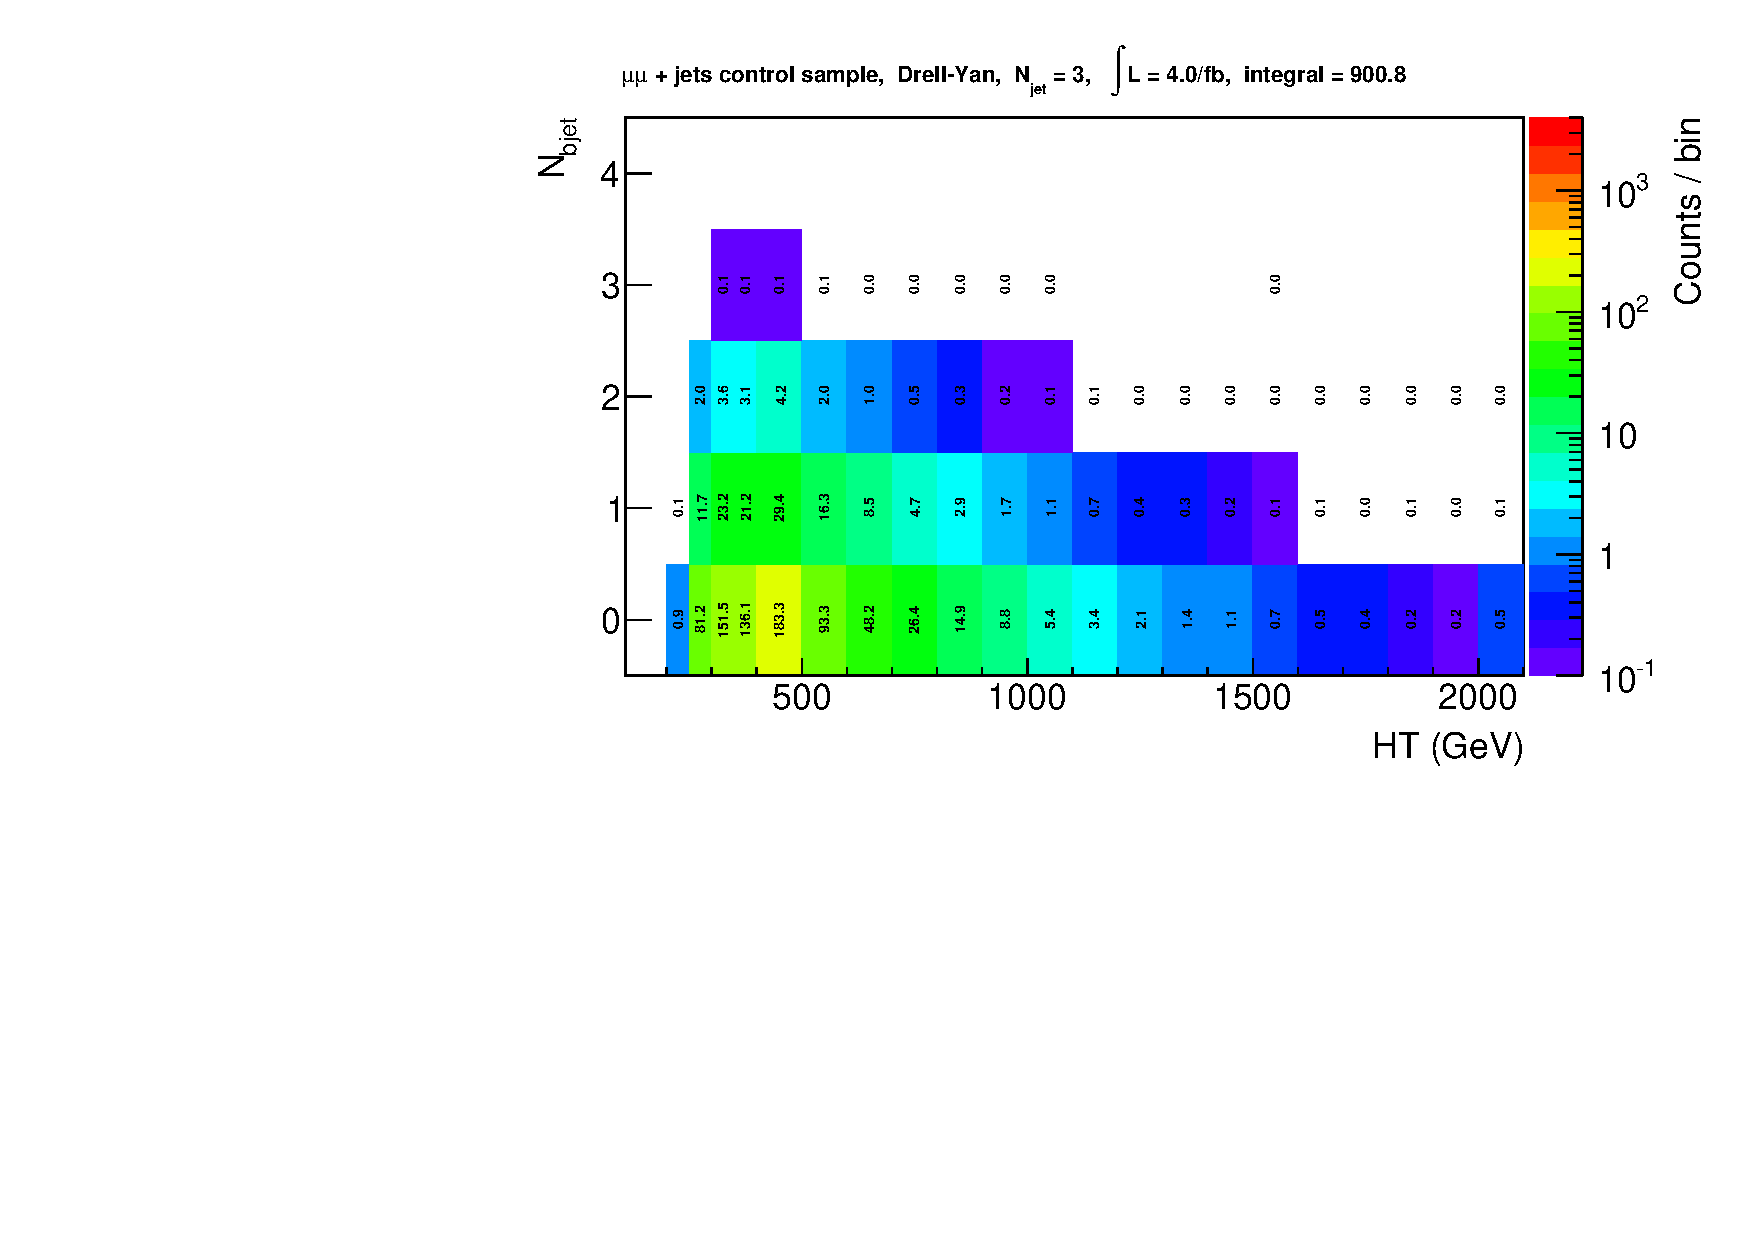
\includegraphics[width=0.5\textwidth]{figures/yieldPlots/mm_dy_eq3j.pdf}
  }
  \\
  \subfigure[Yields from \texorpdfstring{\mmj}{di-muon plus jets} control sample
  ($\njet = 4$)]{
    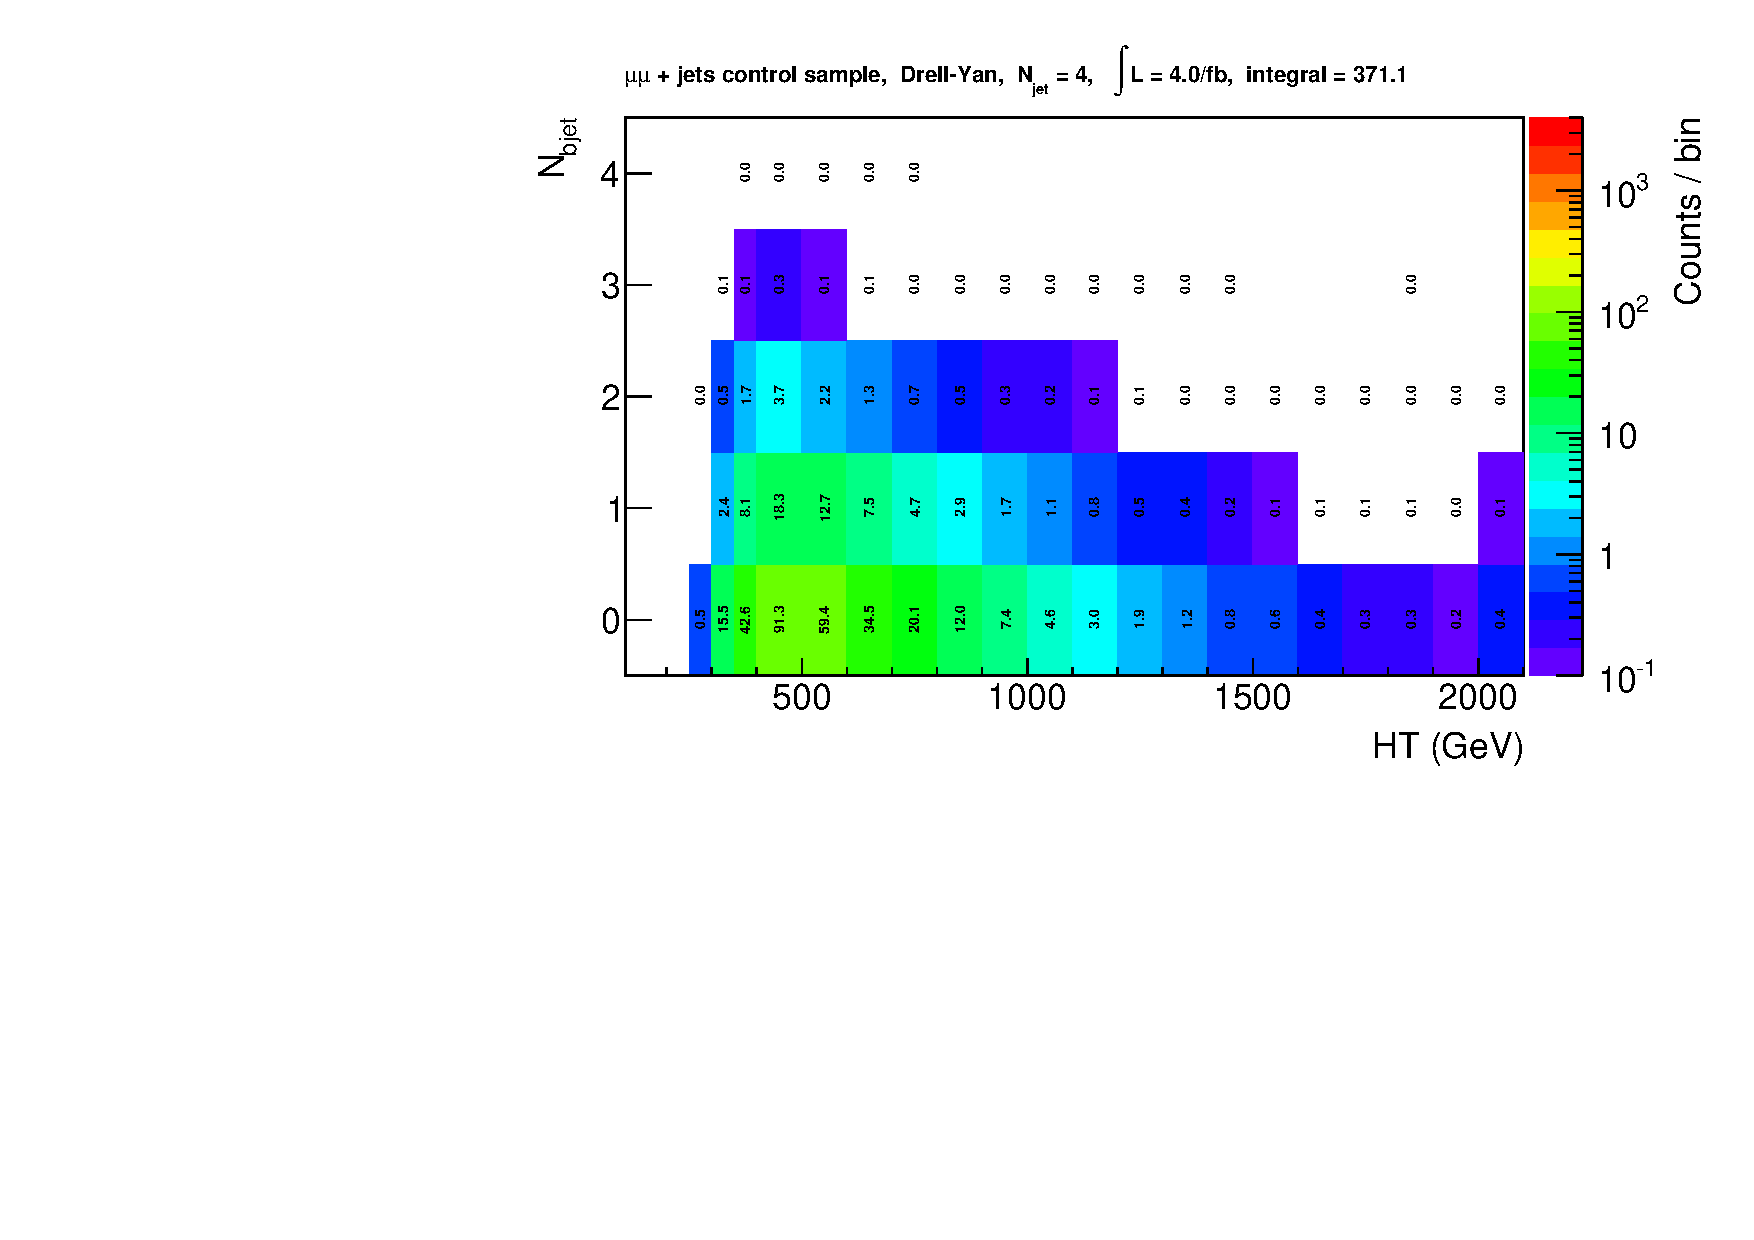
\includegraphics[width=0.5\textwidth]{figures/yieldPlots/mm_dy_eq4j.pdf}
  }~~
  \subfigure[Yields from \texorpdfstring{\mmj}{di-muon plus jets} control sample
  ($\njet \geq 5$)]{
    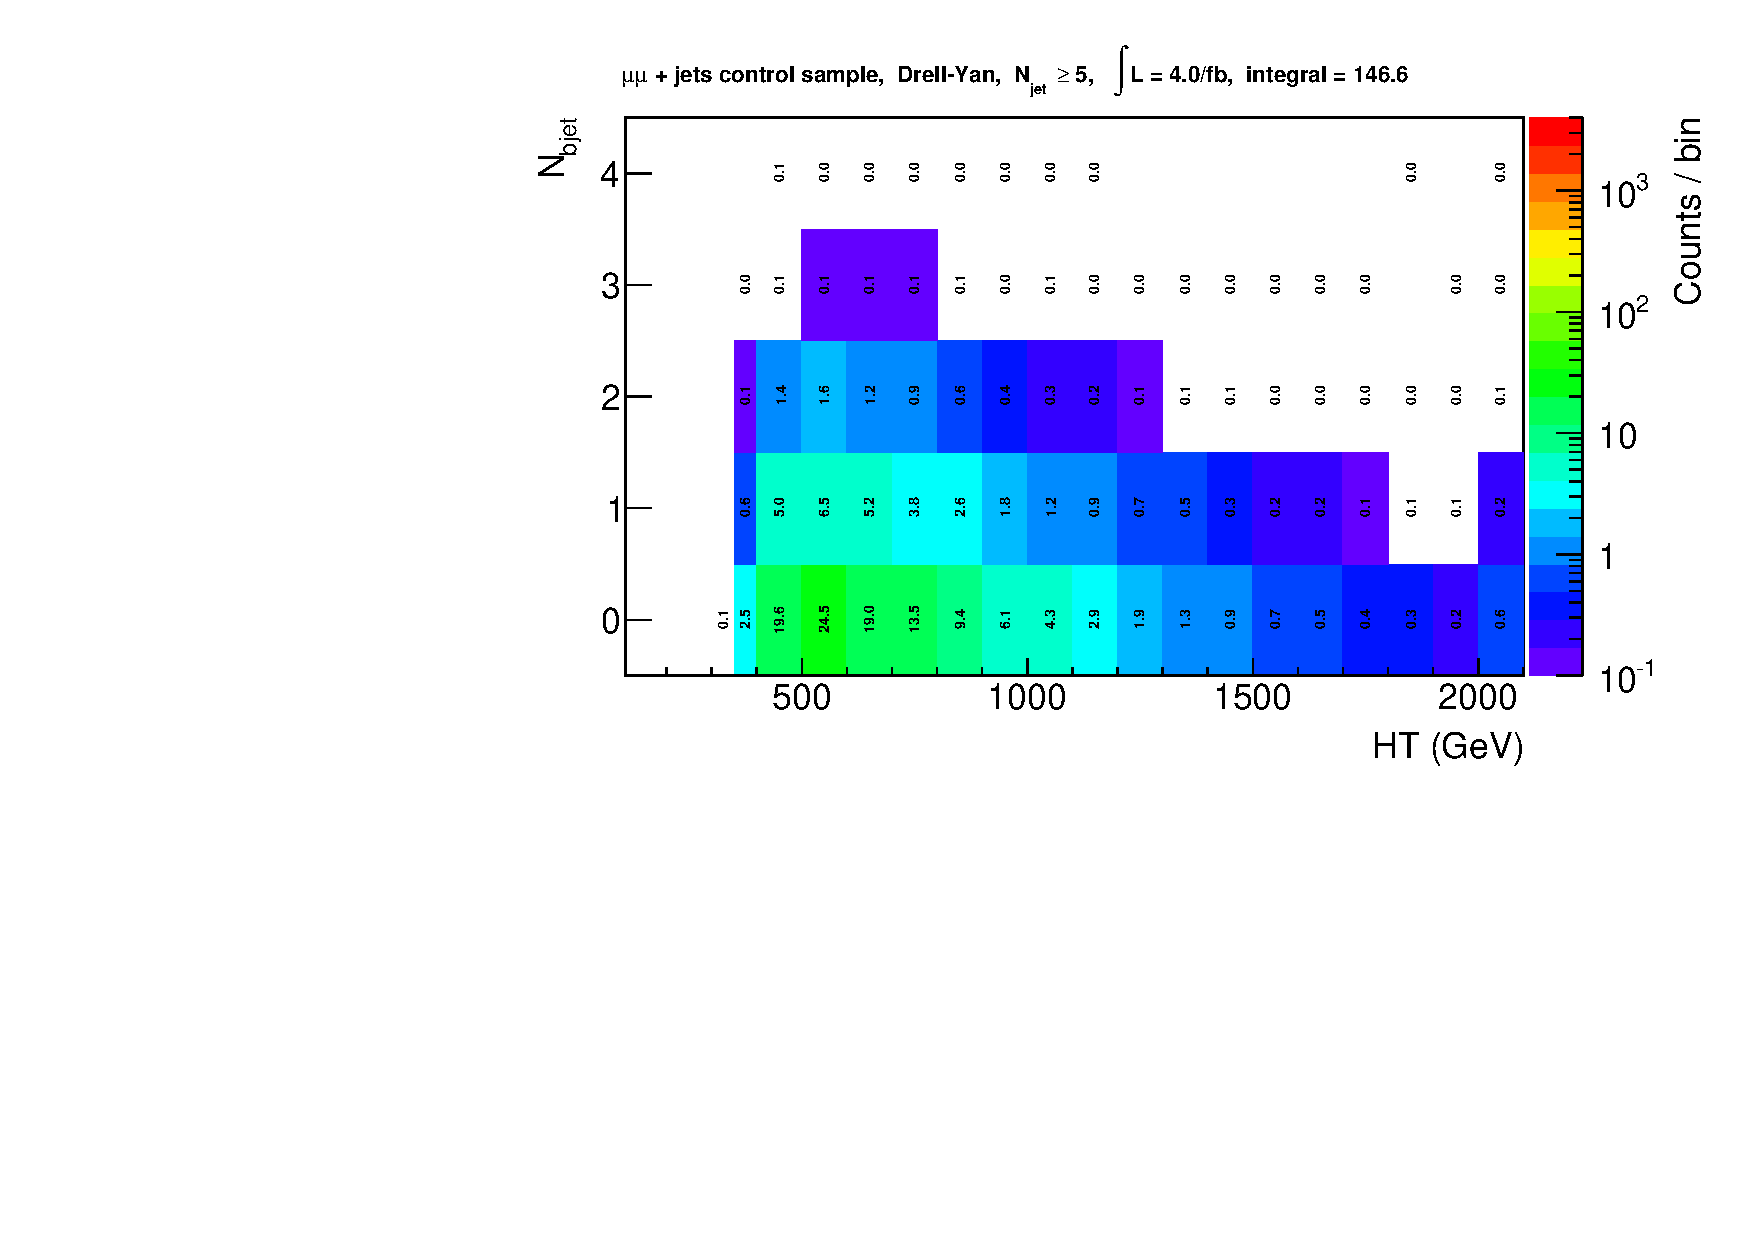
\includegraphics[width=0.5\textwidth]{figures/yieldPlots/mm_dy_ge5j.pdf}
  } 
  \\
  \caption{\label{fig:mumuYields} Yields at $4\fbinv$ for the DY~+~jets MC 
  contributions to the \texorpdfstring{\mmj}{di-muon plus jets} control sample. }
\end{figure}

\begin{figure}[h!]
  \centering
  \subfigure[Yields from \texorpdfstring{\gj}{photon plus jets} control sample
  ($\njet = 2$)]{
    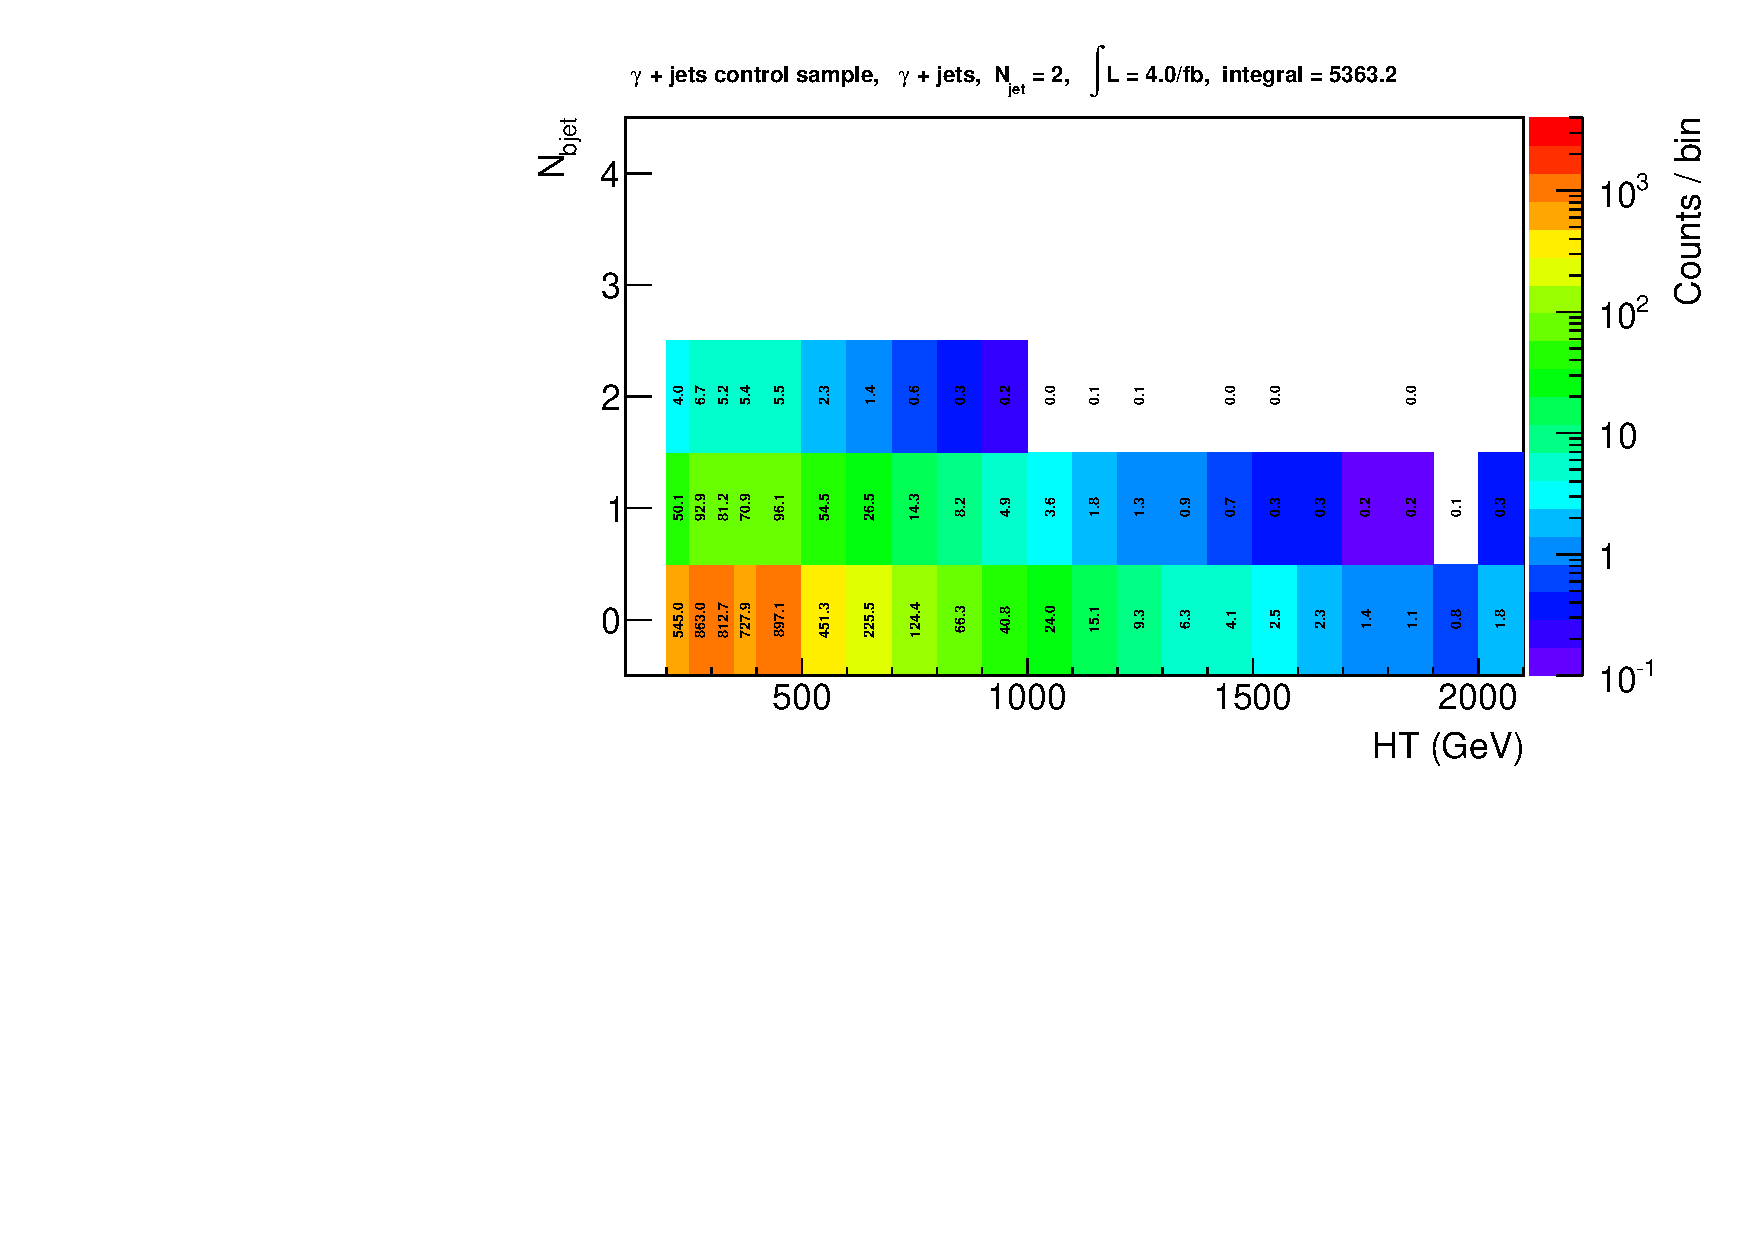
\includegraphics[width=0.5\textwidth]{figures/yieldPlots/ph_gjets_eq2j.pdf}
  }~~
  \subfigure[Yields from \texorpdfstring{\gj}{photon plus jets} control sample
  ($\njet = 3$)]{
    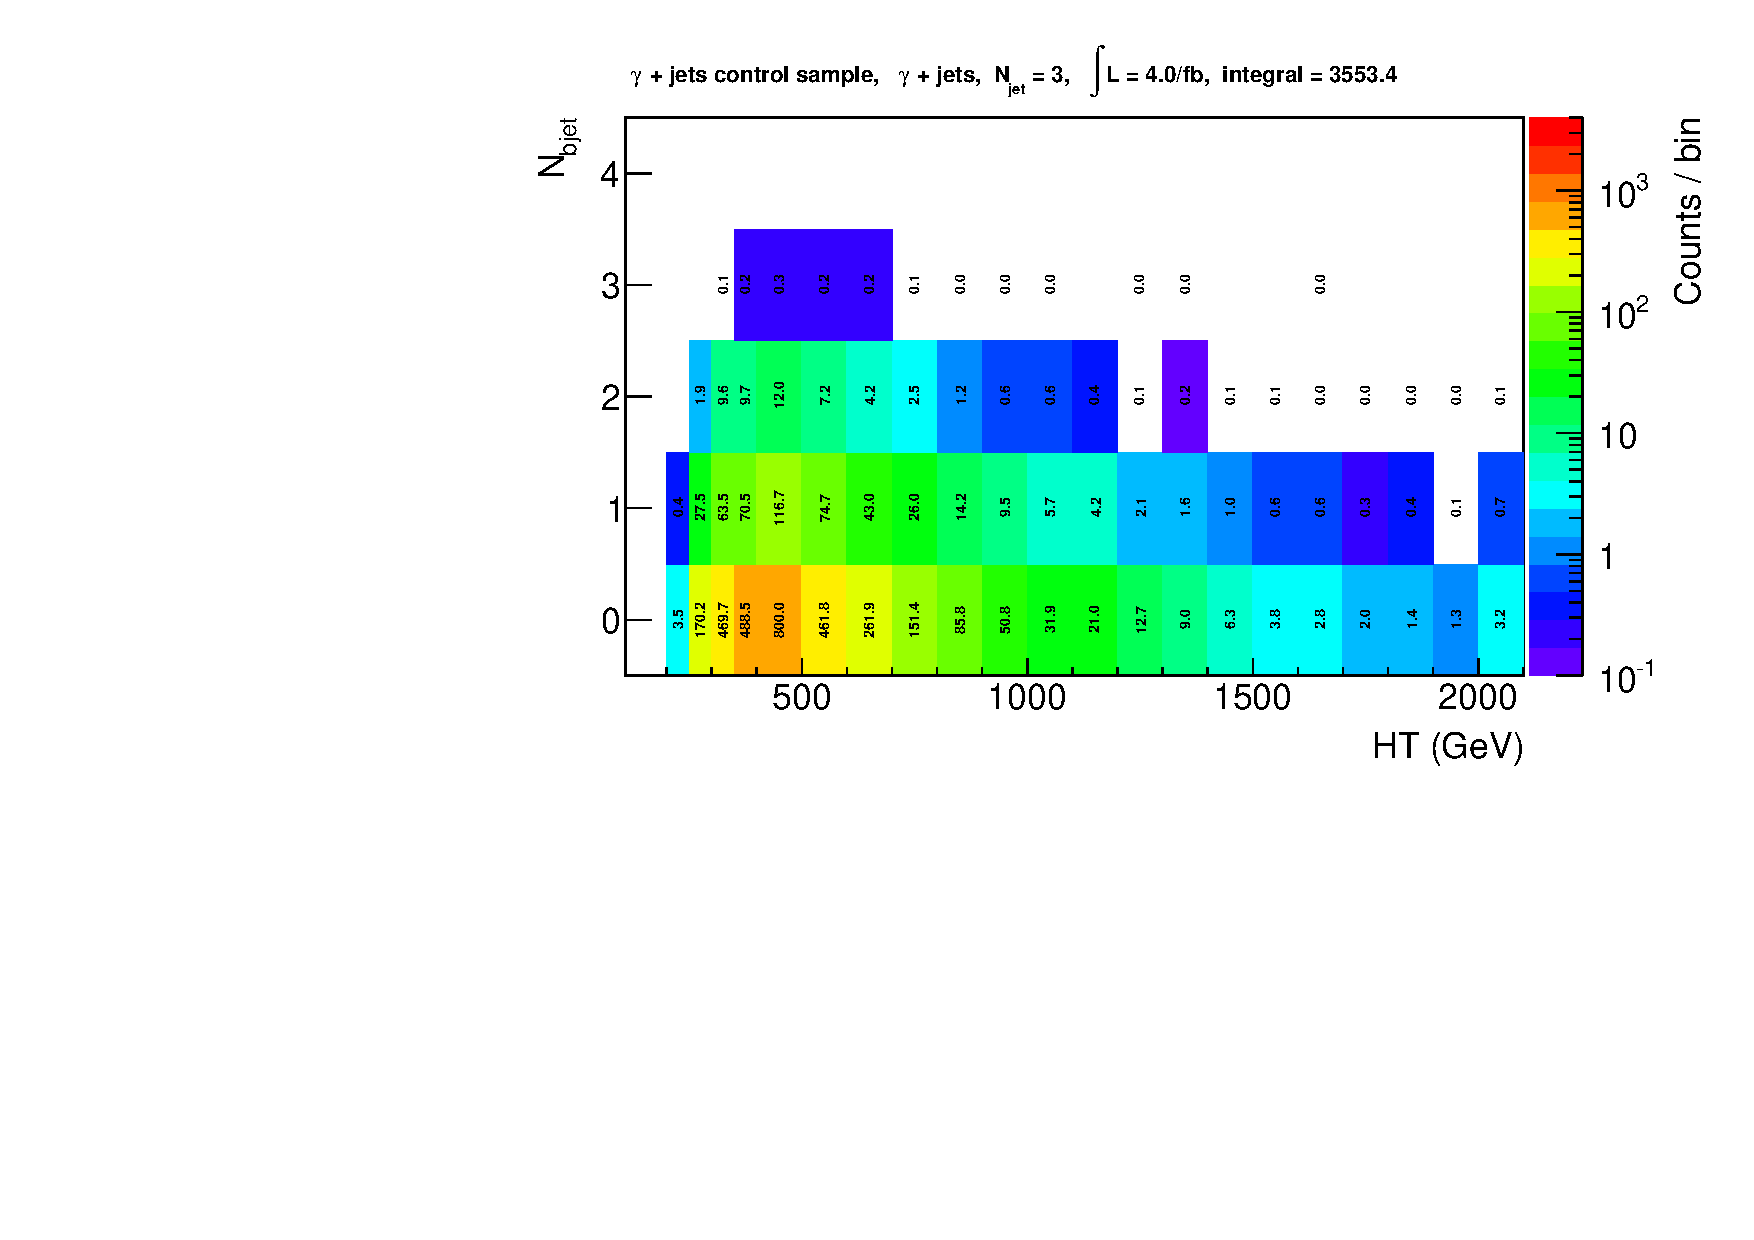
\includegraphics[width=0.5\textwidth]{figures/yieldPlots/ph_gjets_eq3j.pdf}
  }
  \\
  \subfigure[Yields from \texorpdfstring{\gj}{photon plus jets} control sample
  ($\njet = 4$)]{
    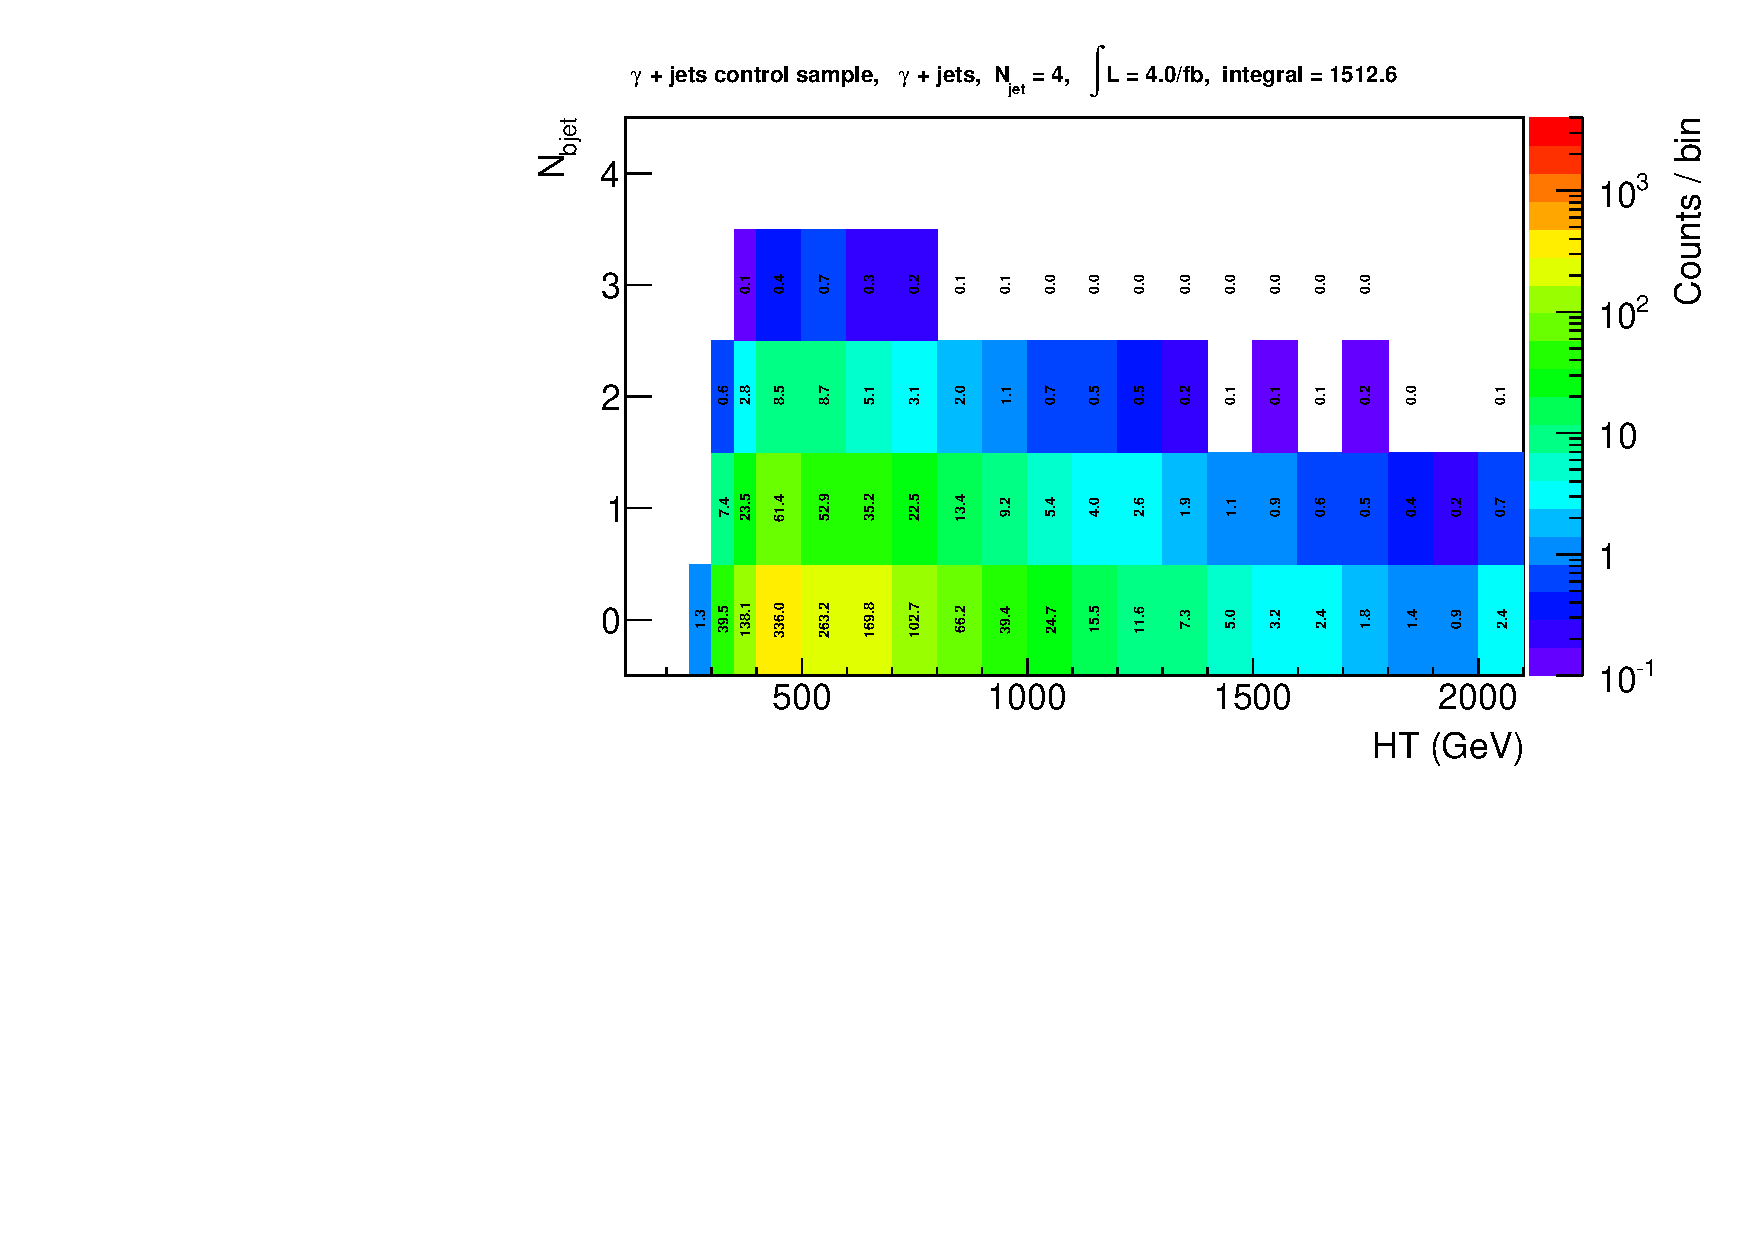
\includegraphics[width=0.5\textwidth]{figures/yieldPlots/ph_gjets_eq4j.pdf}
  }~~
  \subfigure[Yields from \texorpdfstring{\gj}{photon plus jets} control sample
  ($\njet \geq 5$)]{
    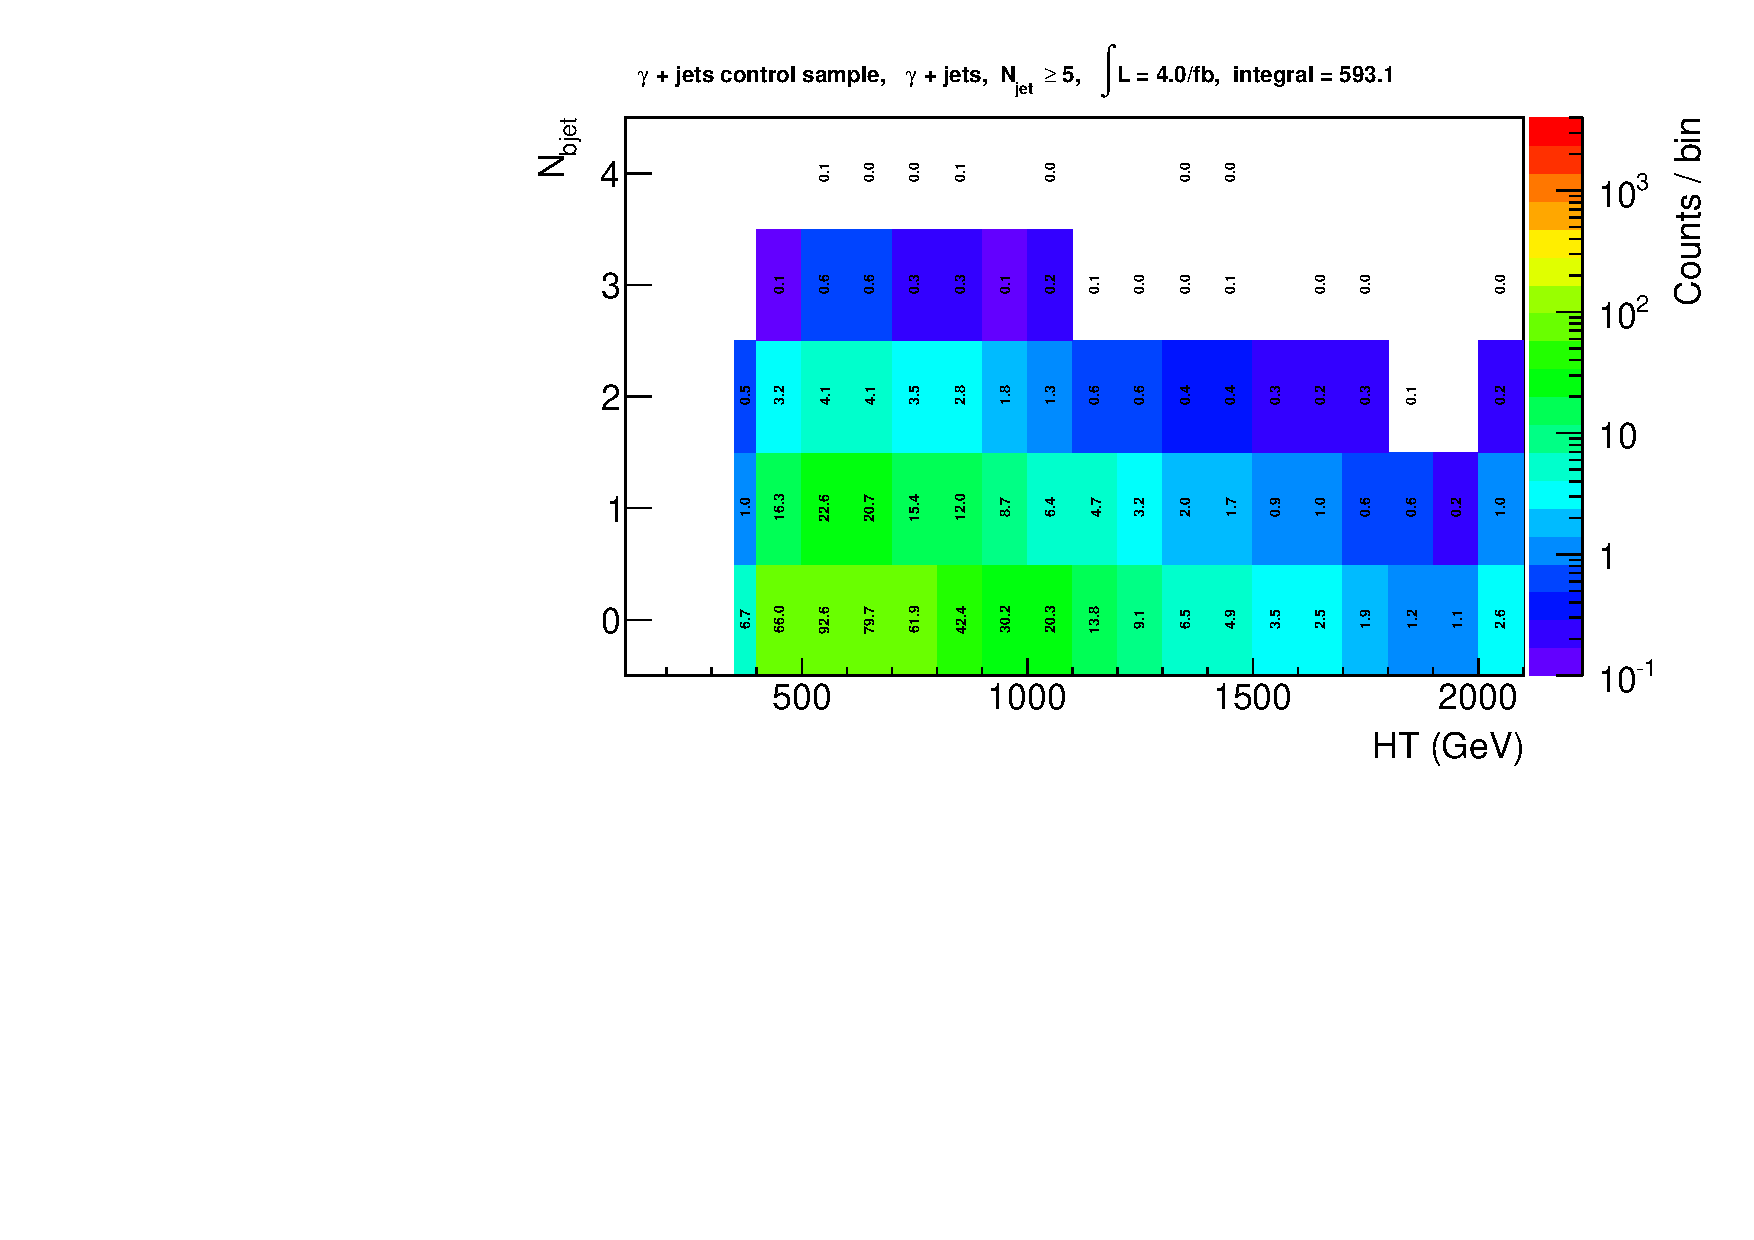
\includegraphics[width=0.5\textwidth]{figures/yieldPlots/ph_gjets_ge5j.pdf}
  } 
  \\
  \caption{\label{fig:gammaYields} Yields at $4\fbinv$ for the GJets MC 
  contributions to the \texorpdfstring{\gj}{photon plus jets} control sample. }
\end{figure}

%%____________________________________________________________________________||
\subsection{The improvement of sensitivity to SUSY and DM models with binning changes}

\subsubsection{Signal }\label{sec:asym_bin}

For a typical compressed model, Fig.~\ref{fig:asymMotivation} shows the second jet \PT
distribution for two different \HT bins. In the low \HT case a large portion of
the events are killed by requiring the second jet to have $\ET>100\gev$. 

We therefore add an new analysis category where the leading jet is required to fulfil 
momenta of jet $\ET>100\gev$ and sub-leading jet $40\gev<\ET<100\gev$. This new category 
results in new asymmetric jet bins split also in $\njet$, $\nb$ and \HT. The asymmetric jet bin
results in much larger acceptance for monojet-type and ISR induced event topologies like DM signals
and compresses SUSY scenarios. 
For the simplified model T2tt with $m_{stop}=425\gev$ and $m_{LSP}=325\gev$, 
including these bins increases signal acceptance by around a factor 3, for the DM models a factor of five is observed.
The asymmetric bins will be added to the nominal selection, thus in combination the for all models the analysis power can only improve or remain constant.
\begin{figure}[h!]
  \centering
  \subfigure[Second jet \PT for $200\gev<\HT<250\gev$, $\alphat>0.65$]{
    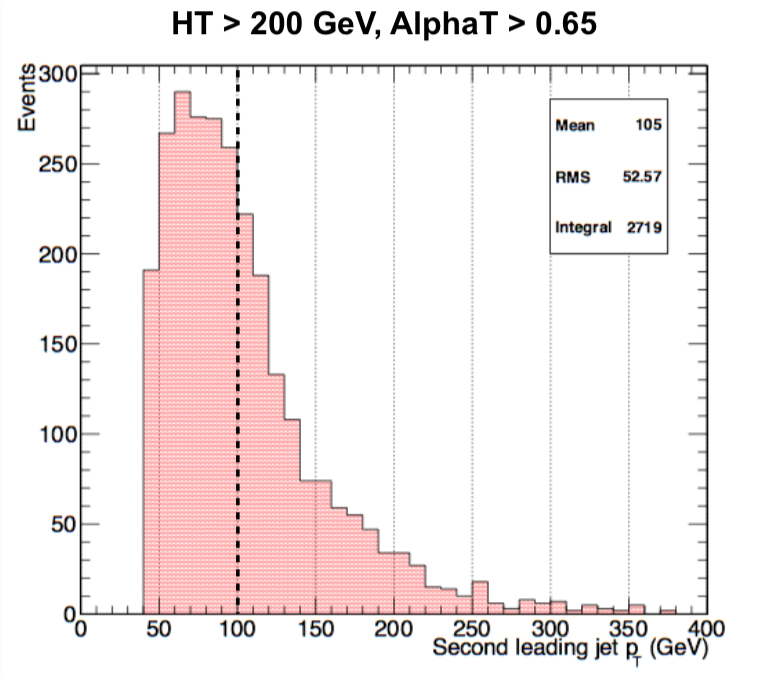
\includegraphics[width=0.5\textwidth]{figures/asymPlots/secondJetPtlowHT}
  }~~
  \subfigure[Second jet \PT for $400\gev<\HT>500\gev$, $\alphat>0.52$]{
    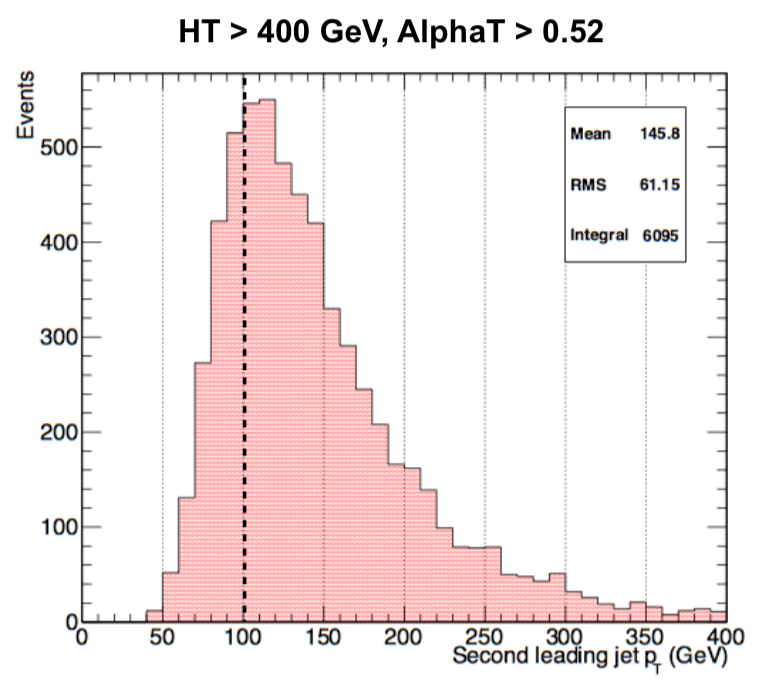
\includegraphics[width=0.5\textwidth]{figures/asymPlots/secondJetPthigherHT}
  }
  \\
  \caption{\label{fig:asymMotivation} The second leading jet \PT for different
  cases of \HT after a baseline signal selection: $\njet\geq2$, lead jet
  $\ET>100\gev$, lepton vetoes. Made with the T2tt ($m_{STOP}=425\gev$, $m_{LSP}=325\gev$) simplified model sample.}
\end{figure}

\subsubsection{Extension of \HT bins}

The production of heavy SUSY particles, such as gluino pair
production, will result in large values of \HT . This is illustrated in the high 
\HT of events in Fig.~\ref{fig:sigYields}. To increase the sensitivity
of the analysis to these kinds of models, the \HT bins can be extended to higher
values. The only limit placed on this value is that there are enough events in the
relevant control samples, to allow a data driven background prediction. The
number of events is deemed to be sufficient when their statistical uncertainty is
approximately equal to the expected systematic uncertainty for the bin in
question. Initial studies suggest it should be possible to extend up to
$\HT=1600$, possibly even $\HT=2000$. This would give a great increase in the
signal over background ratio, particularly for gluino mediated models.

\clearpage
%%____________________________________________________________________________||
\subsection{Signal yields for the asymmetric selection}
The effect of the asymmetric bins designed to increase acceptance for monojet-type and ISR induced final stats has been tested using the DM samples defined in Tab.~\ref{tab:datasets_dm}. Details regarding the asymmetric jet categories are given in Sec.~\ref{sec:asym_bin}.
For illustration purposes we consider only the bins up to $H_\textrm{T}=700$~GeV and jet multiplicities up to $n_j=4$ in Tab.~\ref{tab:sig_yields_AVDM_nom}-\ref{tab:sig_yields_VDM_asym}.

\begin{table}[h]
\topcaption{Signal yields for $H_\textrm{T}$ up to 700~GeV and up to 4 jets in the nominal selection for the axial-vector DM sample.}
\small
\begin{tabular}{lllllllll}
\hline \hline
$H_\textrm{T}$                 &     200 &            250 &             300&             350&             400&             500&             600&             700  \\\hline\hline
$2j 0b$&          16 (0.04)&	   25 (0.03)&	   24 (0.03)&	   19 (0.03)&	   24 (0.03)&	   14 (0.04)&	    7 (0.05)&	    5 (0.07) \\\hline
$2j 1b$&           1 (0.13)&	    2 (0.10)&	    2 (0.10)&	    2 (0.11)&	    3 (0.08)&	    2 (0.12)&	    1 (0.16)&	    1 (0.20) \\\hline
$2j 2b$&           0 (0.50)&	    0 (0.50)&	    0 (0.38)&	    0 (0.41)&	    0 (0.45)&	    0 (0.58)&	    0 (0.58)&	    0 (1.00) \\\hline
$3j 0b$&           0 ( nan)&	    5 (0.07)&	   14 (0.04)&	   18 (0.03)&	   31 (0.03)&	   20 (0.03)&	   13 (0.04)&	    8 (0.05) \\\hline
$3j 1b$&           0 ( nan)&	    0 (0.21)&	    2 (0.12)&	    2 (0.10)&	    4 (0.07)&	    3 (0.09)&	    2 (0.10)&	    1 (0.12) \\\hline
$3j 2b$&           0 ( nan)&	    0 (1.00)&	    0 (0.30)&	    0 (0.30)&	    1 (0.20)&	    0 (0.23)&	    0 (0.32)&	    0 (0.38) \\\hline
$3j 3b$&           0 ( nan)&	    0 ( nan)&	    0 ( nan)&	    0 ( nan)&	    0 ( nan)&	    0 ( nan)&	    0 (1.00)&	    0 (1.00) \\\hline
$4j 0b$&           0 ( nan)&	    0 (0.71)&	    1 (0.13)&	    6 (0.06)&	   15 (0.04)&	   15 (0.04)&	   10 (0.05)&	    7 (0.06) \\\hline
$4j 1b$&           0 ( nan)&	    0 ( nan)&	    0 (0.33)&	    1 (0.17)&	    3 (0.09)&	    2 (0.09)&	    2 (0.11)&	    2 (0.12) \\\hline
$4j 2b$&           0 ( nan)&	    0 ( nan)&	    0 (1.00)&	    0 (0.41)&	    0 (0.22)&	    0 (0.22)&	    0 (0.25)&	    0 (0.50) \\\hline
$4j 3b$&           0 ( nan)&	    0 ( nan)&	    0 ( nan)&	    0 ( nan)&	    0 ( nan)&	    0 ( nan)&	    0 (1.00)&	    0 ( nan) \\\hline
$4j 4b$&           0 ( nan)&	    0 ( nan)&	    0 ( nan)&	    0 ( nan)&	    0 ( nan)&	    0 ( nan)&	    0 ( nan)&	    0 ( nan) \\\hline
\hline
\end{tabular}
\label{tab:sig_yields_AVDM_nom}
\end{table}

\begin{table}[h]
\topcaption{Signal yields for $H_\textrm{T}$ up to 700~GeV and up to 4 jets in the asymmetric jet selection for the axial-vector DM sample.}
\begin{tabular}{lllllllll}
\hline \hline
$H_\textrm{T}$                 &     200 &            250 &             300&             350&             400&             500&             600&             700  \\\hline\hline
Asym. $2j 0b$&     66 (0.02)&	   34 (0.02)&	   20 (0.03)&	   12 (0.04)&	   13 (0.04)&	    6 (0.06)&	    2 (0.09)&	    1 (0.14) \\\hline
Asym. $2j 1b$&      5 (0.06)&	    3 (0.08)&	    2 (0.11)&	    1 (0.12)&	    1 (0.13)&	    1 (0.18)&	    0 (0.35)&	    0 (0.45) \\\hline
Asym. $2j 2b$&      0 (0.27)&	    0 (0.33)&	    0 (0.45)&	    0 (0.50)&	    0 (0.41)&	    0 (1.00)&	    0 ( nan)&	    0 (1.00) \\\hline
Asym. $3j 0b$&     15 (0.04)&	   24 (0.03)&	   18 (0.03)&	   10 (0.05)&	    9 (0.05)&	    3 (0.08)&	    1 (0.13)&	    0 (0.24) \\\hline
Asym. $3j 1b$&      2 (0.12)&	    3 (0.09)&	    2 (0.10)&	    1 (0.12)&	    1 (0.14)&	    0 (0.23)&	    0 (0.32)&	    0 (0.50) \\\hline
Asym. $3j 2b$&      0 (0.26)&	    0 (0.25)&	    0 (0.27)&	    0 (0.45)&	    0 (0.33)&	    0 (0.58)&	    0 (1.00)&	    0 ( nan) \\\hline
Asym. $3j 3b$&      0 (1.00)&	    0 ( nan)&	    0 (1.00)&	    0 (1.00)&	    0 ( nan)&	    0 ( nan)&	    0 ( nan)&	    0 ( nan) \\\hline
Asym. $4j 0b$&      0 (0.58)&	    3 (0.09)&	    7 (0.06)&	    6 (0.06)&	    5 (0.06)&	    2 (0.11)&	    1 (0.19)&	    0 (0.27) \\\hline
Asym. $4j 1b$&      0 (1.00)&	    0 (0.28)&	    1 (0.14)&	    1 (0.15)&	    1 (0.17)&	    0 (0.23)&	    0 (0.33)&	    0 (0.58) \\\hline
Asym. $4j 2b$&      0 ( nan)&	    0 (0.50)&	    0 (0.30)&	    0 (0.41)&	    0 (0.58)&	    0 (0.71)&	    0 (0.71)&	    0 ( nan) \\\hline
Asym. $4j 3b$&      0 ( nan)&	    0 (1.00)&	    0 ( nan)&	    0 ( nan)&	    0 ( nan)&	    0 ( nan)&	    0 ( nan)&	    0 ( nan) \\\hline
Asym. $4j 4b$&      0 ( nan)&	    0 ( nan)&	    0 ( nan)&	    0 ( nan)&	    0 ( nan)&	    0 ( nan)&	    0 ( nan)&	    0 ( nan) \\\hline
\hline              
\end{tabular}
\label{tab:sig_yields_AVDM_asym}
\end{table}





\begin{table}[h]
\topcaption{Signal yields for $H_\textrm{T}$ up to 700~GeV and up to 4 jets in the nominal selection for the vector DM sample.}
\small
\begin{tabular}{lllllllll}
\hline \hline
$H_\textrm{T}$                 &     200 &            250 &             300&             350&             400&             500&             600&             700  \\\hline\hline
$2j 0b$&          16 (0.04)&	   31 (0.03)&	   31 (0.03)&	   24 (0.03)&	   36 (0.02)&	   21 (0.03)&	   12 (0.04)&	    9 (0.05) \\\hline
$2j 1b$&           1 (0.13)&	    3 (0.09)&	    3 (0.08)&	    3 (0.08)&	    5 (0.07)&	    3 (0.08)&	    2 (0.11)&	    1 (0.12) \\\hline
$2j 2b$&           0 (0.58)&	    0 (0.28)&	    0 (0.35)&	    0 (0.50)&	    0 (0.28)&	    0 (0.33)&	    0 (0.58)&	    0 (0.58) \\\hline
$3j 0b$&           0 (0.41)&	    6 (0.06)&	   18 (0.03)&	   23 (0.03)&	   42 (0.02)&	   30 (0.03)&	   19 (0.03)&	   13 (0.04) \\\hline
$3j 1b$&           0 ( nan)&	    1 (0.18)&	    2 (0.09)&	    3 (0.08)&	    7 (0.05)&	    6 (0.06)&	    4 (0.07)&	    3 (0.09) \\\hline
$3j 2b$&           0 ( nan)&	    0 (0.58)&	    0 (0.41)&	    0 (0.21)&	    1 (0.16)&	    0 (0.21)&	    0 (0.23)&	    0 (0.24) \\\hline
$3j 3b$&           0 ( nan)&	    0 ( nan)&	    0 ( nan)&	    0 ( nan)&	    0 ( nan)&	    0 (1.00)&	    0 (1.00)&	    0 ( nan) \\\hline
$4j 0b$&           0 ( nan)&	    0 (1.00)&	    2 (0.11)&	    6 (0.06)&	   21 (0.03)&	   20 (0.03)&	   14 (0.04)&	   10 (0.04) \\\hline
$4j 1b$&           0 ( nan)&	    0 ( nan)&	    0 (0.23)&	    1 (0.14)&	    4 (0.07)&	    4 (0.07)&	    3 (0.08)&	    2 (0.09) \\\hline
$4j 2b$&           0 ( nan)&	    0 ( nan)&	    0 (0.58)&	    0 (0.50)&	    1 (0.18)&	    1 (0.19)&	    1 (0.19)&	    1 (0.20) \\\hline
$4j 3b$&           0 ( nan)&	    0 ( nan)&	    0 ( nan)&	    0 ( nan)&	    0 ( nan)&	    0 (0.50)&	    0 (0.71)&	    0 ( nan) \\\hline
$4j 4b$&           0 ( nan)&	    0 ( nan)&	    0 ( nan)&	    0 ( nan)&	    0 ( nan)&	    0 ( nan)&	    0 ( nan)&	    0 ( nan) \\\hline
\hline
\end{tabular}
\label{tab:sig_yields_VDM_nom}
\end{table}

\begin{table}[h]
\topcaption{Signal yields for $H_\textrm{T}$ up to 700~GeV and up to 4 jets in the asymmetric jet selection for the vector DM sample.}
\begin{tabular}{lllllllll}
\hline \hline
$H_\textrm{T}$                 &     200 &            250 &             300&             350&             400&             500&             600&             700  \\\hline\hline
Asym. $2j 0b$&     71 (0.02)&	   40 (0.02)&	   26 (0.03)&	   18 (0.03)&	   19 (0.03)&	    9 (0.05)&	    4 (0.07)&	    3 (0.09) \\\hline
Asym. $2j 1b$&      6 (0.06)&	    4 (0.07)&	    3 (0.09)&	    2 (0.10)&	    2 (0.10)&	    1 (0.14)&	    1 (0.16)&	    0 (0.24) \\\hline
Asym. $2j 2b$&      0 (0.21)&	    0 (0.28)&	    0 (0.45)&	    0 (0.58)&	    0 (0.33)&	    0 (0.58)&	    0 ( nan)&	    0 (1.00) \\\hline
Asym. $3j 0b$&     18 (0.03)&	   29 (0.03)&	   22 (0.03)&	   13 (0.04)&	   13 (0.04)&	    5 (0.06)&	    2 (0.09)&	    1 (0.13) \\\hline
Asym. $3j 1b$&      2 (0.11)&	    4 (0.07)&	    3 (0.08)&	    2 (0.11)&	    2 (0.10)&	    1 (0.15)&	    0 (0.22)&	    0 (0.27) \\\hline
Asym. $3j 2b$&      0 (0.29)&	    0 (0.27)&	    0 (0.23)&	    0 (0.28)&	    0 (0.32)&	    0 (0.50)&	    0 (0.71)&	    0 ( nan) \\\hline
Asym. $3j 3b$&      0 ( nan)&	    0 ( nan)&	    0 ( nan)&	    0 ( nan)&	    0 ( nan)&	    0 ( nan)&	    0 ( nan)&	    0 ( nan) \\\hline
Asym. $4j 0b$&      0 (0.58)&	    3 (0.08)&	    9 (0.05)&	    9 (0.05)&	    8 (0.05)&	    3 (0.08)&	    1 (0.13)&	    1 (0.17) \\\hline
Asym. $4j 1b$&      0 ( nan)&	    1 (0.17)&	    1 (0.13)&	    2 (0.12)&	    2 (0.12)&	    0 (0.20)&	    0 (0.32)&	    0 (0.41) \\\hline
Asym. $4j 2b$&      0 ( nan)&	    0 (0.58)&	    0 (0.35)&	    0 (0.24)&	    0 (0.32)&	    0 (0.50)&	    0 (1.00)&	    0 (0.71) \\\hline
Asym. $4j 3b$&      0 ( nan)&	    0 ( nan)&	    0 ( nan)&	    0 (1.00)&	    0 (1.00)&	    0 (1.00)&	    0 ( nan)&	    0 ( nan) \\\hline
Asym. $4j 4b$&      0 ( nan)&	    0 ( nan)&	    0 ( nan)&	    0 ( nan)&	    0 ( nan)&	    0 ( nan)&	    0 ( nan)&	    0 ( nan) \\\hline
\hline
\end{tabular}
\label{tab:sig_yields_VDM_asym}
\end{table}


One see that the acceptance gained in addition to the nominal selection is typically about a factor of five larger and mainly in low $H_\textrm{T}$ and jet multiplicity bin.
However, the background expectation for this additional bins are also increasing as seen in Tab. .

Figures~\ref{fig:DM_AV_Yields1}-~\ref{fig:DM_V_Yields2} show the yields obtained for the nominal and asymmetric selection for all $H_\textrm{T}$ and jet multiplicities.

\begin{figure}[]
  \centering
  \subfigure[Hadronic signal region yields for the axial vector DM model, nominal selection.
  ($\njet = 2$)]{
    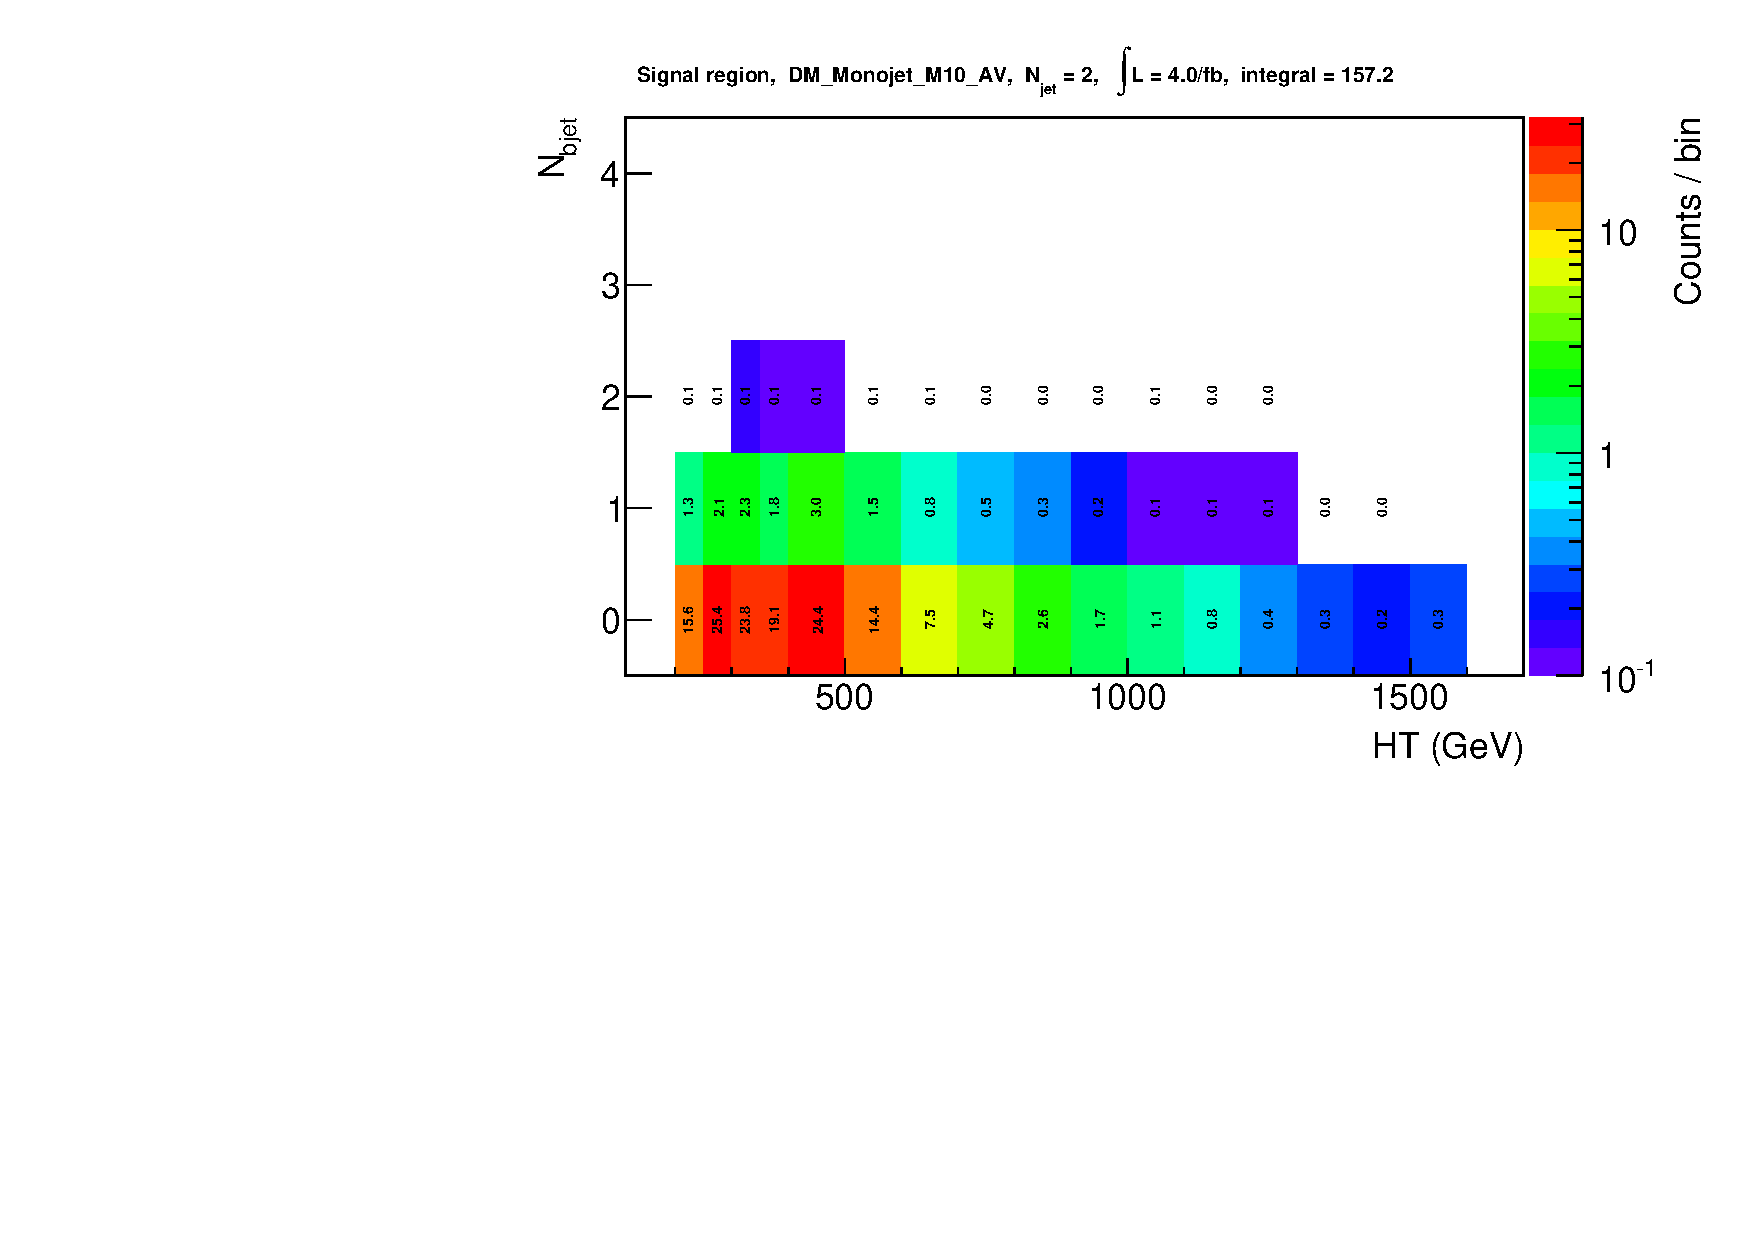
\includegraphics[width=0.5\textwidth]{figures/yieldPlots/sig_DM_Monojet_M10_AV_eq2j.pdf}
  }~~
  \subfigure[Hadronic signal region yields for the axial vector DM model, asymmetric selection.
  ($\njet = 2$)]{
    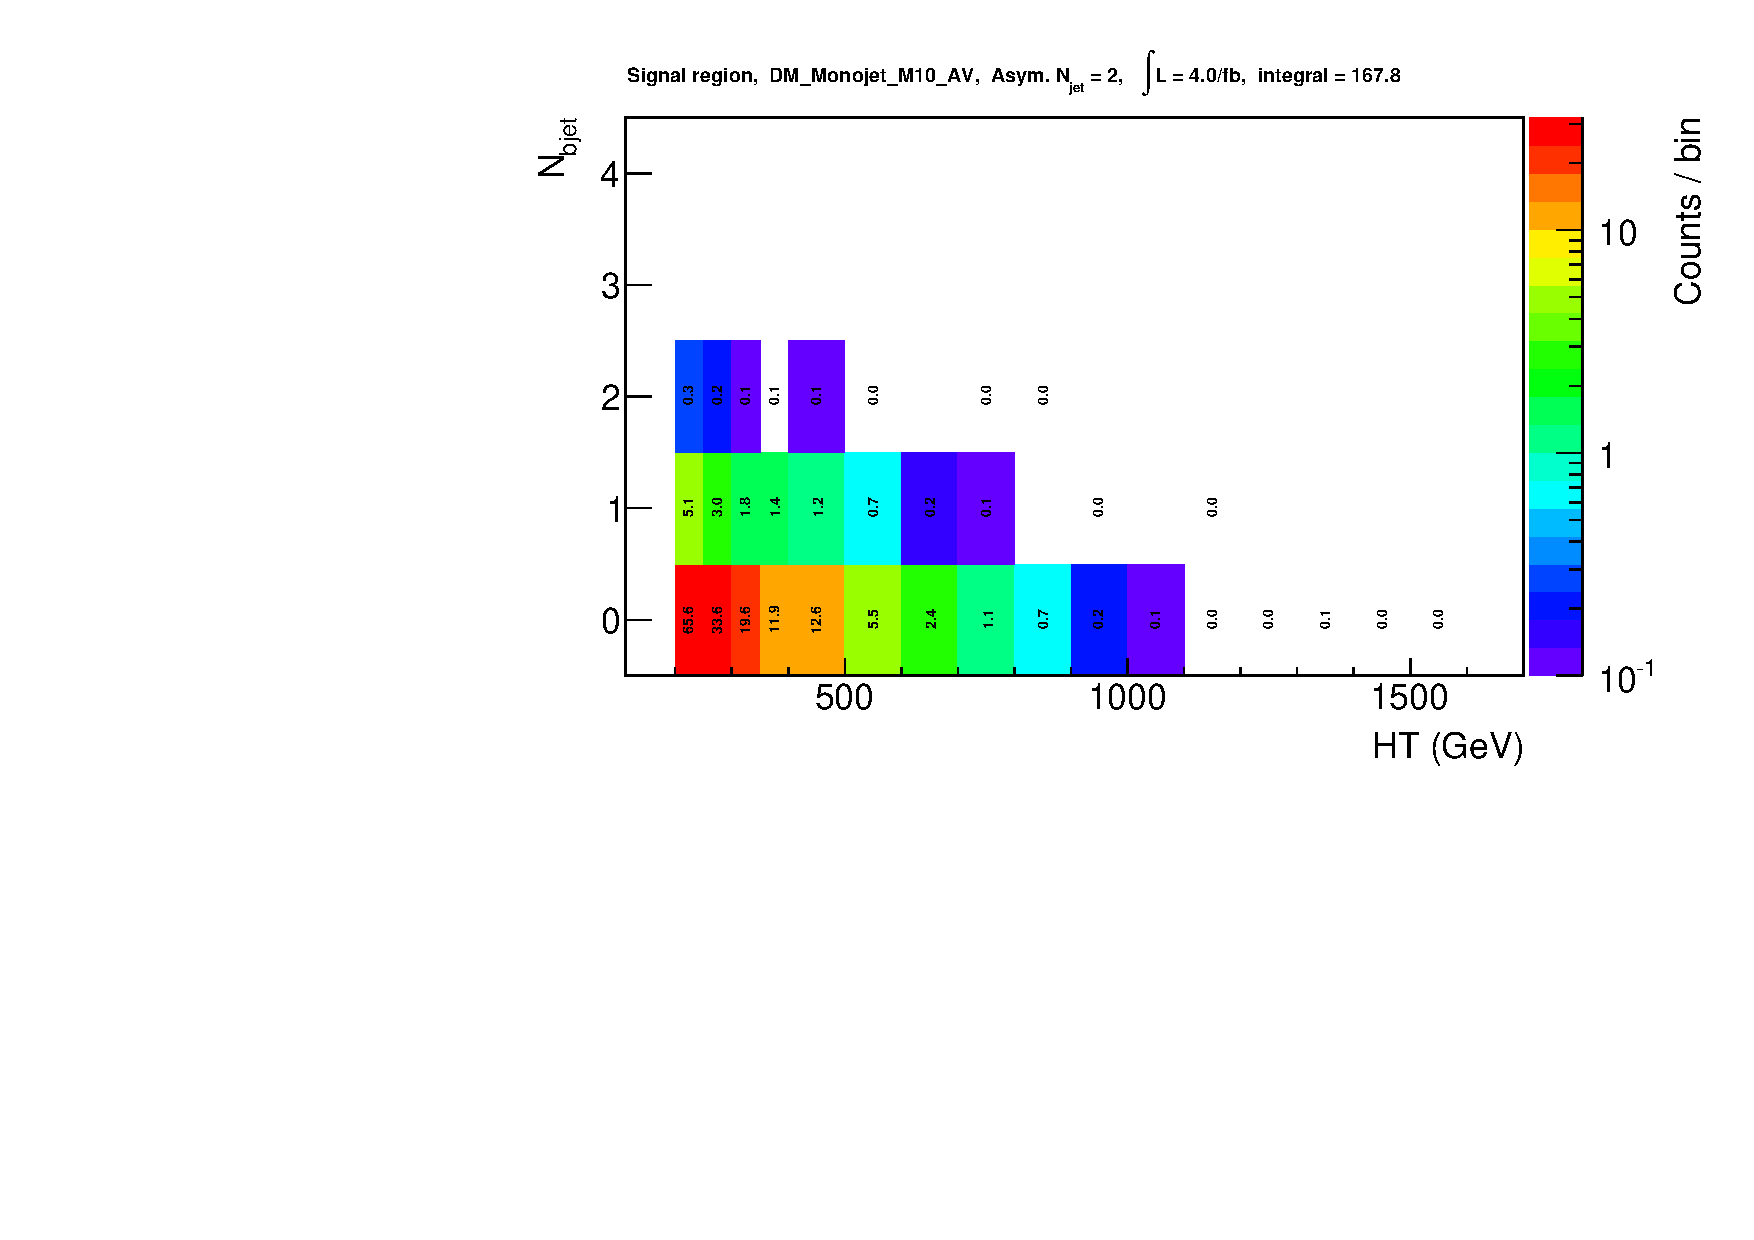
\includegraphics[width=0.5\textwidth]{figures/yieldPlots/sig_DM_Monojet_M10_AV_eq2jAsym.pdf}
  }\\

  \subfigure[Hadronic signal region yields for the axial vector DM model, nominal selection.
  ($\njet = 2$)]{
    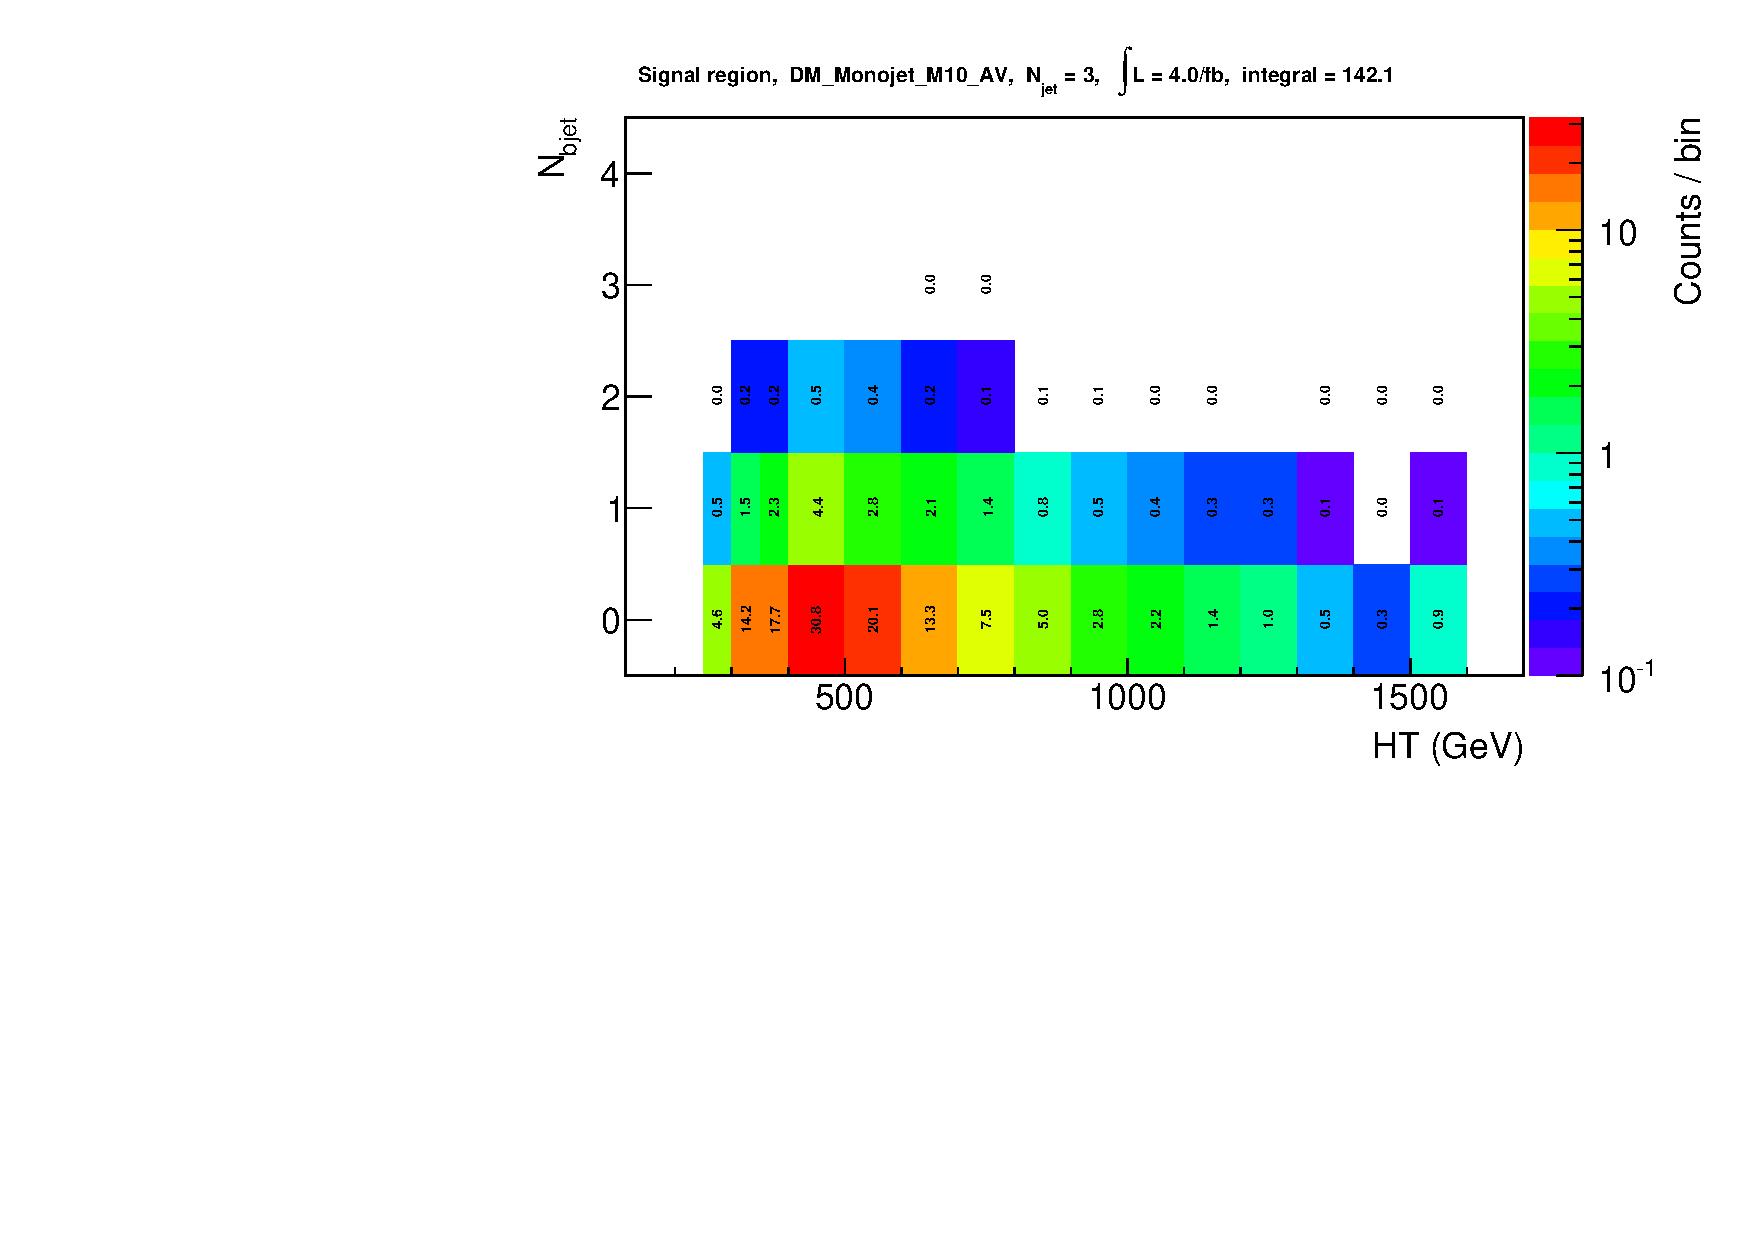
\includegraphics[width=0.5\textwidth]{figures/yieldPlots/sig_DM_Monojet_M10_AV_eq3j.pdf}
  }~~
  \subfigure[Hadronic signal region yields for the axial vector DM model, asymmetric selection.
  ($\njet = 2$)]{
    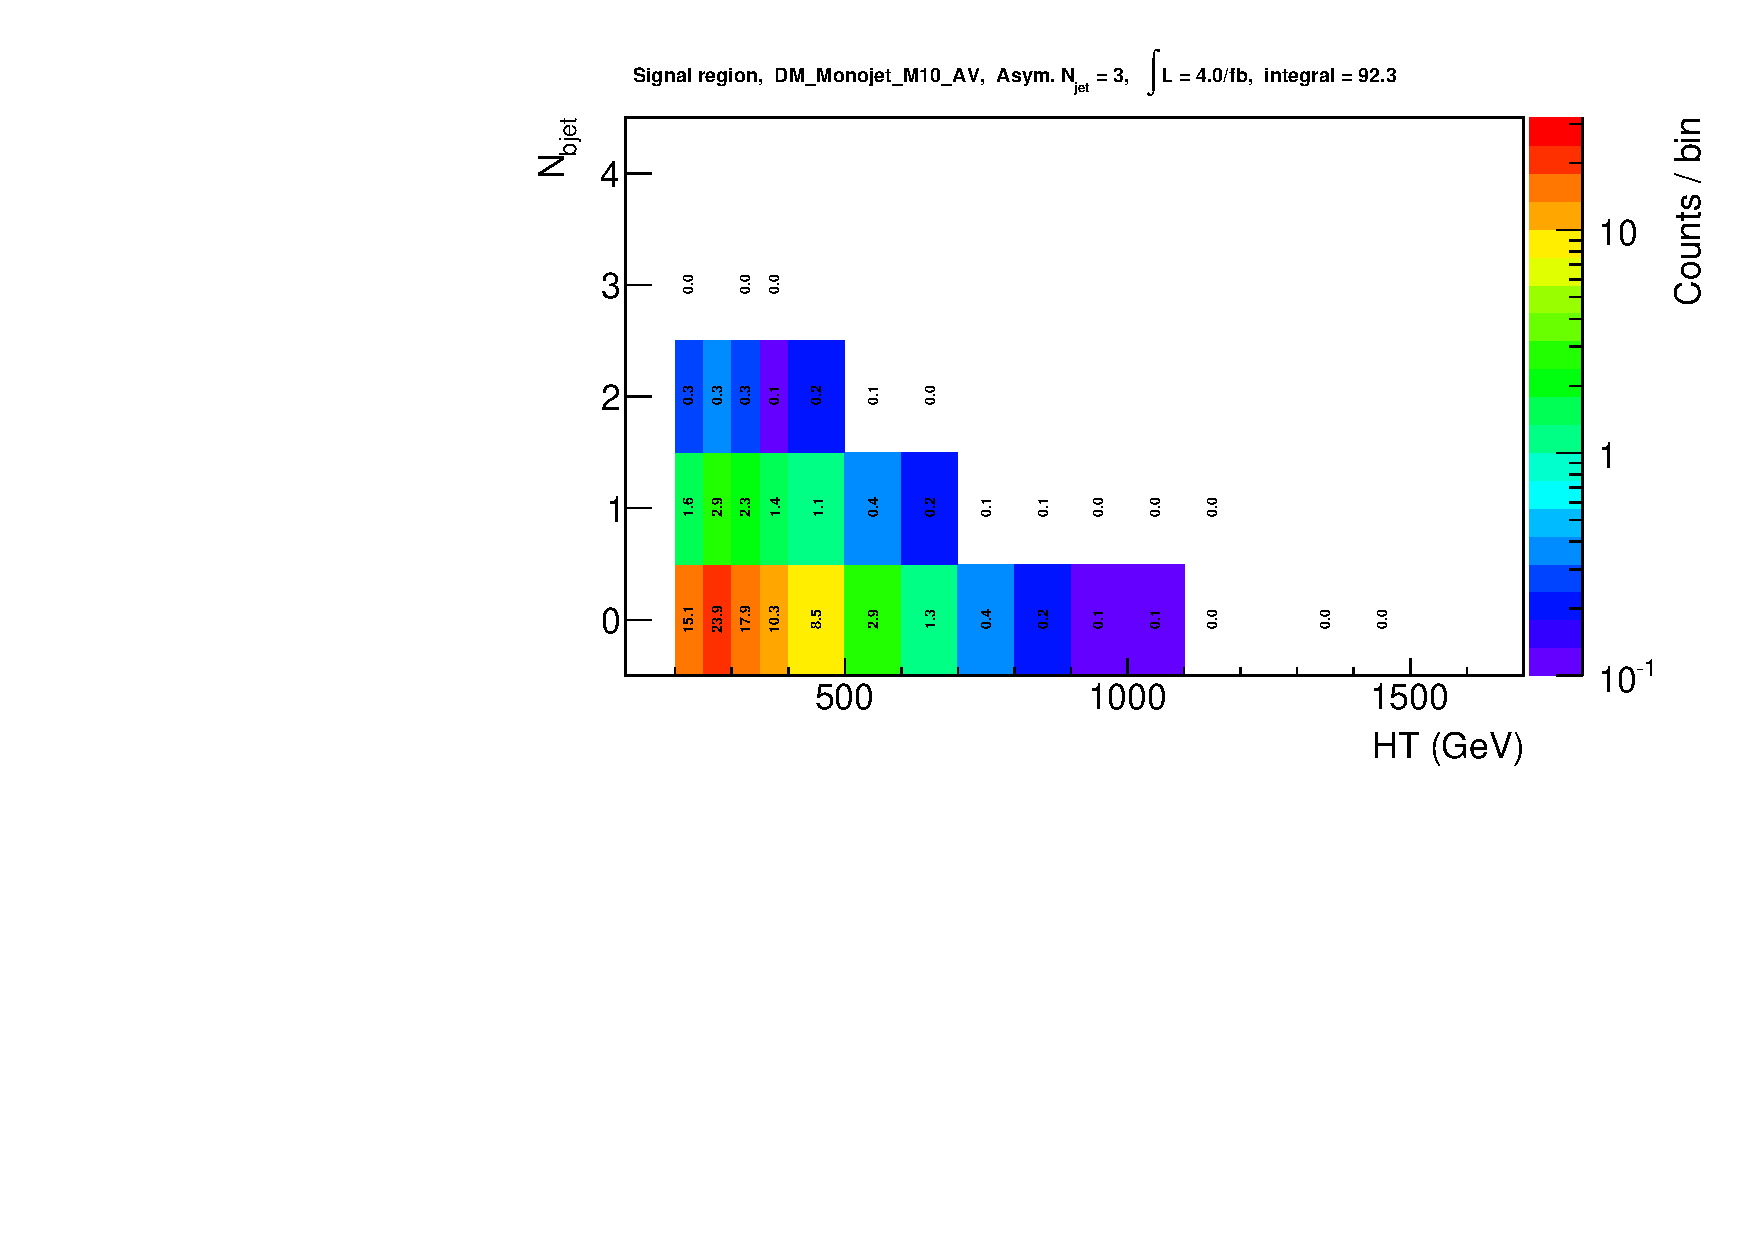
\includegraphics[width=0.5\textwidth]{figures/yieldPlots/sig_DM_Monojet_M10_AV_eq3jAsym.pdf}
  }\\
  \caption{\label{fig:DM_AV_Yields1} Yields at $4\fbinv$ for the AV DM model in the
  hadronic signal region, for $\njet=2,3$. The binning corresponds to the analysis  bins. }
\end{figure}



\begin{figure}[]
  \centering
  \subfigure[Hadronic signal region yields for the axial vector DM model, nominal selection.
  ($\njet = 2$)]{
    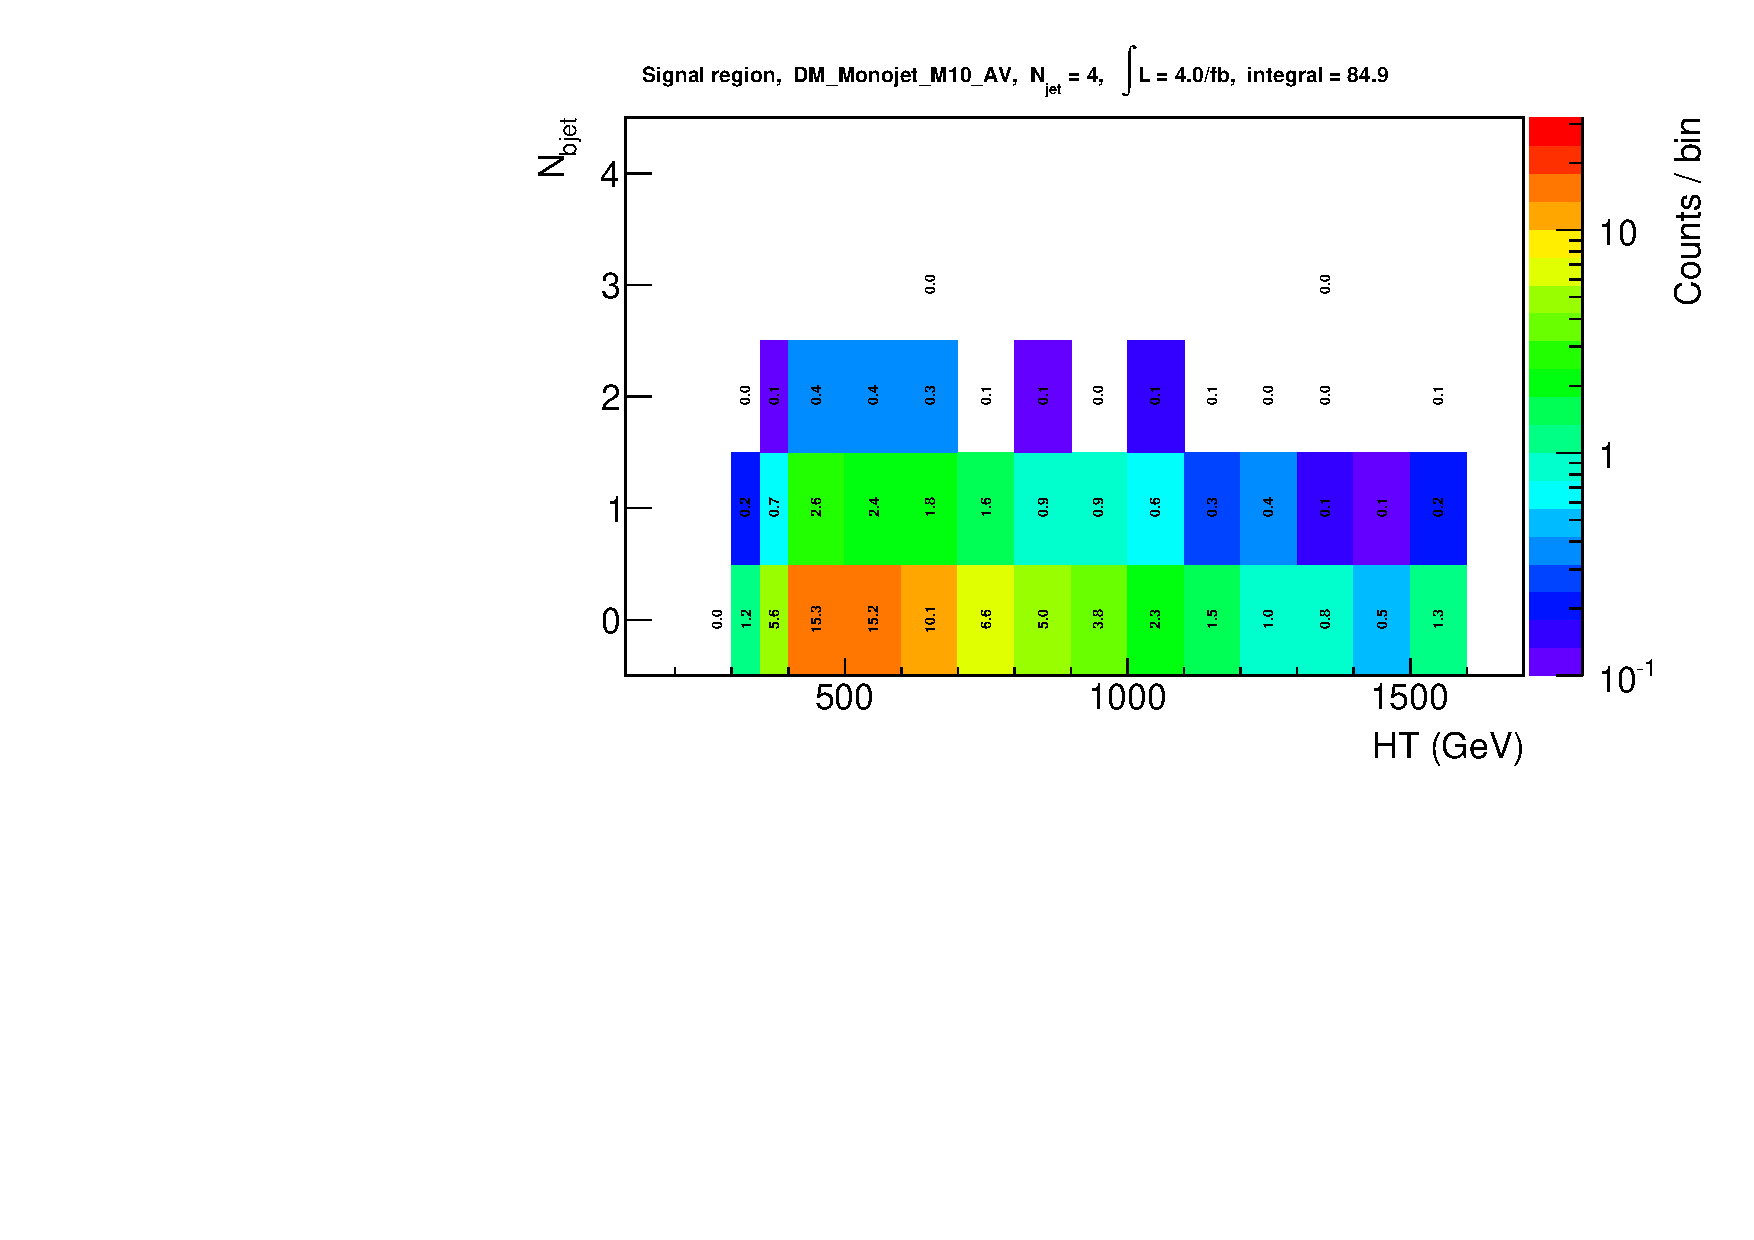
\includegraphics[width=0.5\textwidth]{figures/yieldPlots/sig_DM_Monojet_M10_AV_eq4j.pdf}
  }~~
  \subfigure[Hadronic signal region yields for the axial vector DM model, asymmetric selection.
  ($\njet = 2$)]{
    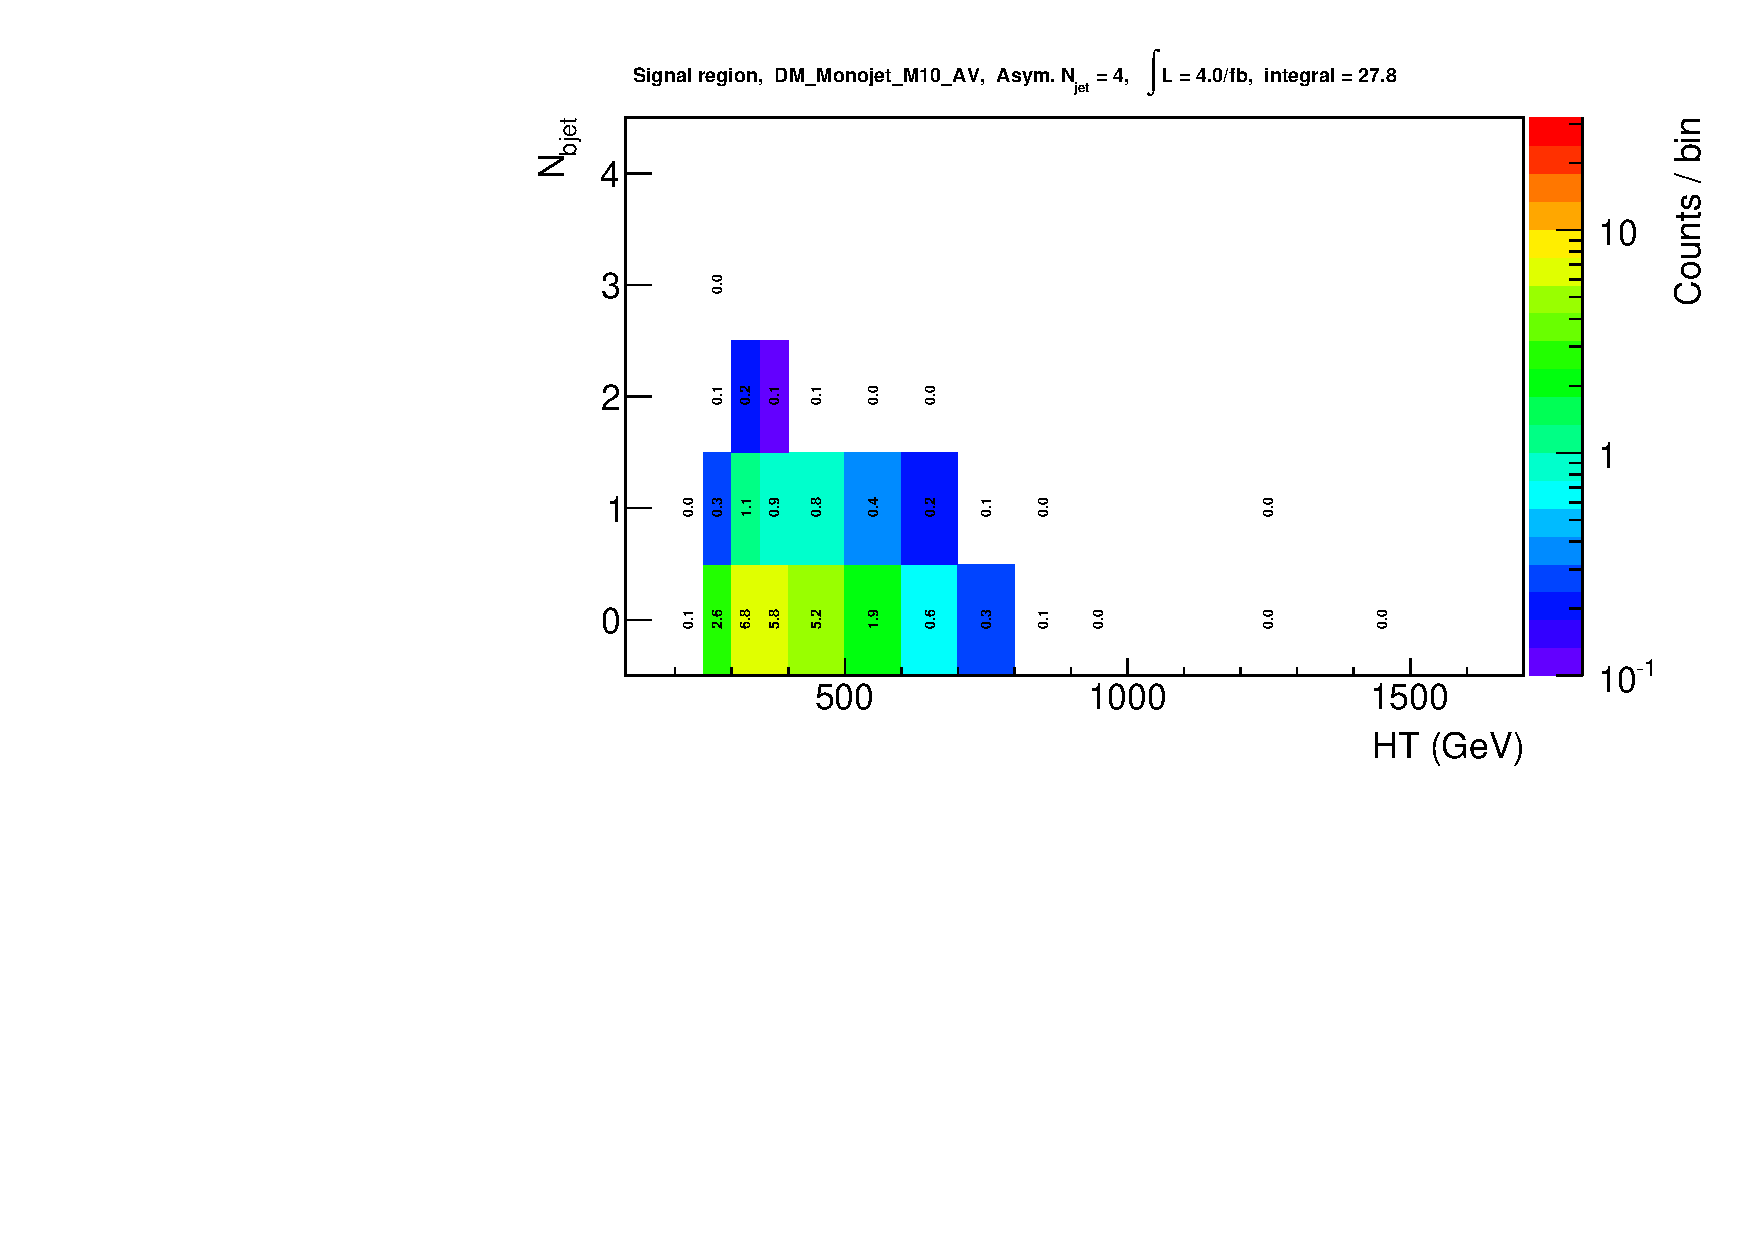
\includegraphics[width=0.5\textwidth]{figures/yieldPlots/sig_DM_Monojet_M10_AV_eq4jAsym.pdf}
  }\\

  \subfigure[Hadronic signal region yields for the axial vector DM model, nominal selection.
  ($\njet = 5$)]{
    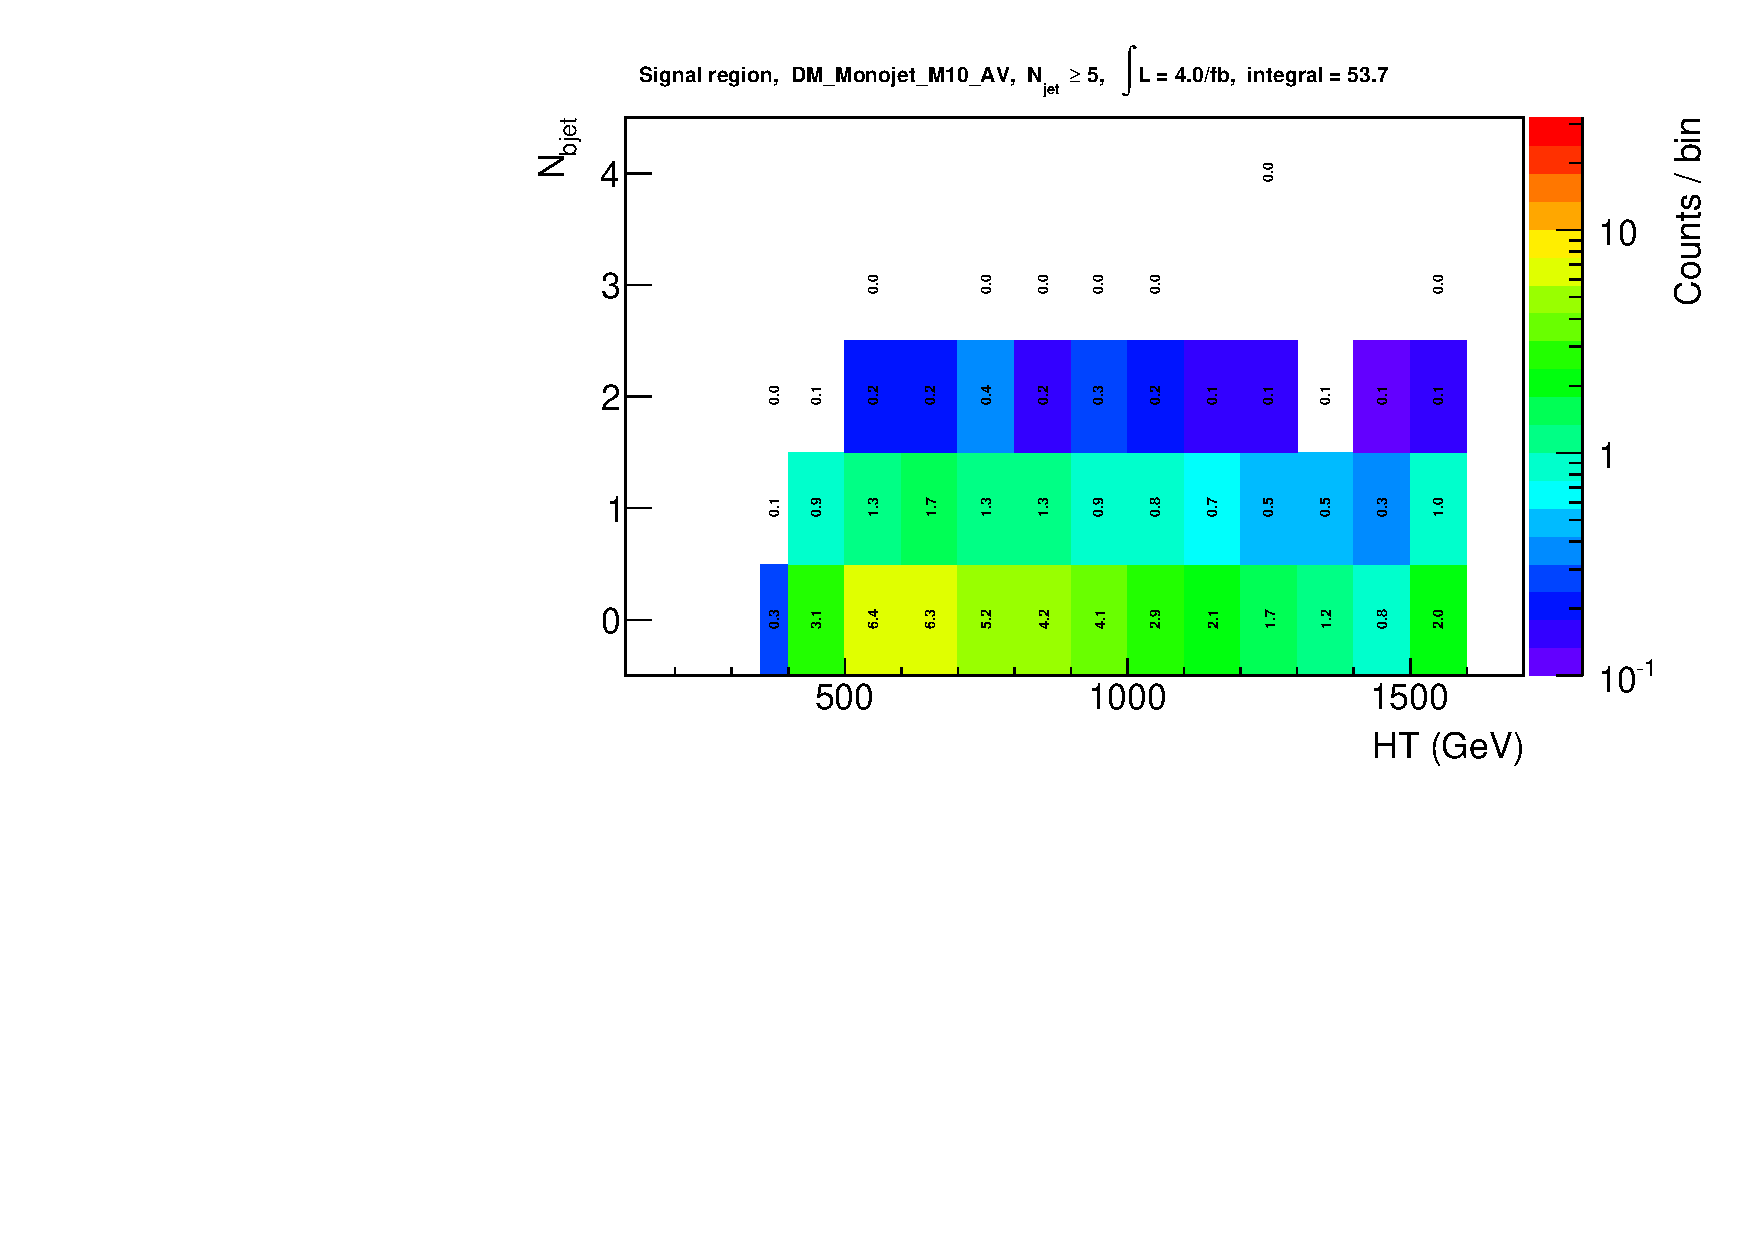
\includegraphics[width=0.5\textwidth]{figures/yieldPlots/sig_DM_Monojet_M10_AV_ge5j.pdf}
  }~~
  \subfigure[Hadronic signal region yields for the axial vector DM model, asymmetric selection.
  ($\njet = 5$)]{
    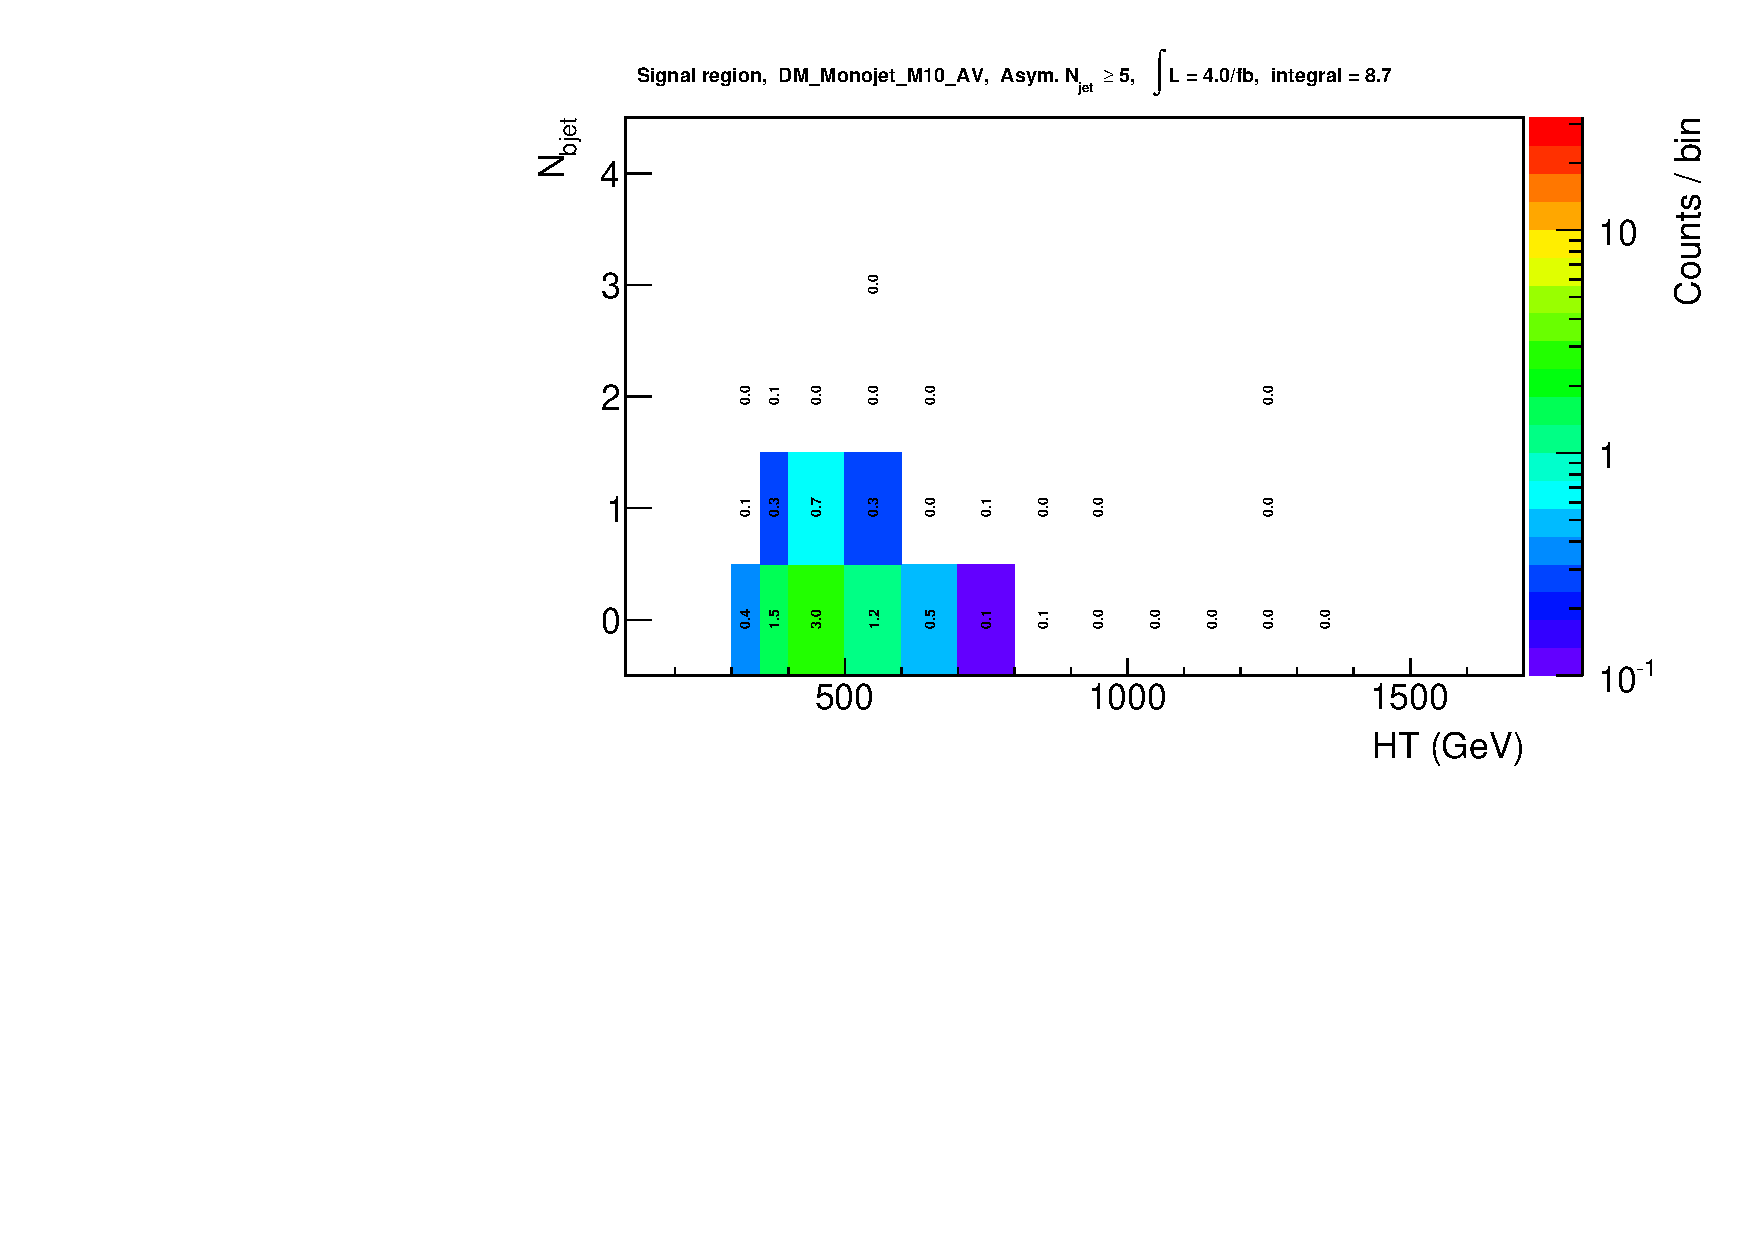
\includegraphics[width=0.5\textwidth]{figures/yieldPlots/sig_DM_Monojet_M10_AV_ge5jAsym.pdf}
  }
  \caption{\label{fig:DM_AV_Yields2} Yields at $4\fbinv$ for the AV DM in the
  hadronic signal region, for $\njet=4,5$. The binning corresponds to the analysis  bins. }
\end{figure}




\begin{figure}[]
  \centering
  \subfigure[Hadronic signal region yields for the axial vector DM model, nominal selection.
  ($\njet = 2$)]{
    \includegraphics[width=0.5\textwidth]{figures/yieldPlots/sig_DM_Monojet_M1000_V_eq2j.pdf}
  }~~
  \subfigure[Hadronic signal region yields for the axial vector DM model, asymmetric selection.
  ($\njet = 2$)]{
    \includegraphics[width=0.5\textwidth]{figures/yieldPlots/sig_DM_Monojet_M1000_V_eq2jAsym.pdf}
  }\\

  \subfigure[Hadronic signal region yields for the axial vector DM model, nominal selection.
  ($\njet = 2$)]{
    \includegraphics[width=0.5\textwidth]{figures/yieldPlots/sig_DM_Monojet_M1000_V_eq3j.pdf}
  }~~
  \subfigure[Hadronic signal region yields for the axial vector DM model, asymmetric selection.
  ($\njet = 2$)]{
    \includegraphics[width=0.5\textwidth]{figures/yieldPlots/sig_DM_Monojet_M1000_V_eq3jAsym.pdf}
  }\\
  \caption{\label{fig:DM_V_Yields1} Yields at $4\fbinv$ for the AV DM model in the
  hadronic signal region, for $\njet=2,3$. The binning corresponds to the analysis  bins. }
\end{figure}



\begin{figure}[]
  \centering
  \subfigure[Hadronic signal region yields for the axial vector DM model, nominal selection.
  ($\njet = 2$)]{
    \includegraphics[width=0.5\textwidth]{figures/yieldPlots/sig_DM_Monojet_M1000_V_eq4j.pdf}
  }~~
  \subfigure[Hadronic signal region yields for the axial vector DM model, asymmetric selection.
  ($\njet = 2$)]{
    \includegraphics[width=0.5\textwidth]{figures/yieldPlots/sig_DM_Monojet_M1000_V_eq4jAsym.pdf}
  }\\

  \subfigure[Hadronic signal region yields for the axial vector DM model, nominal selection.
  ($\njet = 5$)]{
    \includegraphics[width=0.5\textwidth]{figures/yieldPlots/sig_DM_Monojet_M1000_V_ge5j.pdf}
  }~~
  \subfigure[Hadronic signal region yields for the axial vector DM model, asymmetric selection.
  ($\njet = 5$)]{
    \includegraphics[width=0.5\textwidth]{figures/yieldPlots/sig_DM_Monojet_M1000_V_ge5jAsym.pdf}
  }
  \caption{\label{fig:DM_V_Yields2} Yields at $4\fbinv$ for the AV DM in the
  hadronic signal region, for $\njet=4,5$. The binning corresponds to the analysis  bins. }
\end{figure}







Corresponding figures for the $Tbbbb$ models are presented in Fig.\ref{fig:Tbbb_Yields2}.%~\ref{fig:Tbbb_Yields1}-~

%no point in showing these as there are no events

%\begin{figure}[]
%  \centering
%  \subfigure[Hadronic signal region yields for the axial vector DM model, nominal selection.
%  ($\njet = 2$)]{
%    \includegraphics[width=0.5\textwidth]{figures/yieldPlots/sig_T1bbbb_eq2j.pdf}
%  }~~
%  \subfigure[Hadronic signal region yields for the axial vectorDM model, asymetric selection.
%  ($\njet = 2$)]{
%    \includegraphics[width=0.5\textwidth]{figures/yieldPlots/sig_T1bbbb_eq2jAsym.pdf}
%  }\\
%
%  \subfigure[Hadronic signal region yields for the axial vector DM model, nominal selection.
%  ($\njet = 2$)]{
%    \includegraphics[width=0.5\textwidth]{figures/yieldPlots/sig_T1bbbb_eq3j.pdf}
%  }~~
%  \subfigure[Hadronic signal region yields for the axial vectorDM model, asymetric selection.
%  ($\njet = 2$)]{
%    \includegraphics[width=0.5\textwidth]{figures/yieldPlots/sig_T1bbbb_eq3jAsym.pdf}
%  }\\
%  \caption{\label{fig:Tbbb_Yields1} Yields at $4\fbinv$ for the $Tbbbb$ model in the
%  hadronic signal region, for $\njet=2,3$. The binning corresponds to the analysis  bins. }
%\end{figure}



\begin{figure}[]
  \centering
  \subfigure[Hadronic signal region yields for the T1bbbb simplified model, nominal selection.
  ($\njet = 4$)]{
    \includegraphics[width=0.5\textwidth]{figures/yieldPlots/sig_T1bbbb_eq4j.pdf}
  }~~
  \subfigure[Hadronic signal region yields for the T1bbbb simplified model, asymmetric selection.
  ($\njet = 4$)]{
    \includegraphics[width=0.5\textwidth]{figures/yieldPlots/sig_T1bbbb_eq4jAsym.pdf}
  }\\

  \subfigure[Hadronic signal region yields for the T1bbbb simplified model, nominal selection.
  ($\njet \geq 5$)]{
    \includegraphics[width=0.5\textwidth]{figures/yieldPlots/sig_T1bbbb_ge5j.pdf}
  }~~
  \subfigure[Hadronic signal region yields for the T1bbbb simplified model, asymmetric selection.
  ($\njet \geq 5$)]{
    \includegraphics[width=0.5\textwidth]{figures/yieldPlots/sig_T1bbbb_ge5jAsym.pdf}
  }
  \caption{\label{fig:Tbbb_Yields2} Yields at $4\fbinv$ for the $T1bbbb$ in the
  hadronic signal region, for $\njet=4,5$. The binning corresponds to the analysis  bins. }
\end{figure}




\clearpage

%%____________________________________________________________________________||


%%____________________________________________________________________________||
\subsection{Background yields for the asymmetric selection}


As in Sec.~\ref{sec:bkgd-comp} the yields are also assessed for the asymmetric jet selection.
The plots presenting the yields for the electroweak backgrounds can be found in in Figs~\ref{fig:ewkYields1}-\ref{fig:ewkYields4}. 
The breakdown of the three dominant background processes,\zInv , \ttbar and $W+\textrm{jets}$, are also presented. 
Other background processes like single top and diboson processes, is found to be negligible and are therefore not 
shown.

\begin{figure}[]
  \centering
  \subfigure[Hadronic signal region yields for electroweak backgrounds
  ($\njet = 2$)]{
    \includegraphics[width=0.5\textwidth]{figures/yieldPlots/had_ewk_eq2jAsym.pdf}
  }~~
  \subfigure[Hadronic signal region yields for the \zInv background
  ($\njet = 2$)]{
    \includegraphics[width=0.5\textwidth]{figures/yieldPlots/had_zinv_eq2jAsym.pdf}
  }\\
  \subfigure[Hadronic signal region yields for W~+~jets background
  ($\njet = 2$)]{
    \includegraphics[width=0.5\textwidth]{figures/yieldPlots/had_wjets_eq2jAsym.pdf}
  }~~
  \subfigure[Hadronic signal region yields for \ttbar background
  ($\njet = 2$)]{
    \includegraphics[width=0.5\textwidth]{figures/yieldPlots/had_ttbar_eq2jAsym.pdf}
  }
  \caption{\label{fig:ewkYields1} Yields at $4\fbinv$ for the electroweak backgrounds in the
  hadronic signal region, $\njet=2$. The binning is chosen to be in line with the analysis
  bins. The contribution from the dominant backgrounds is shown separately.}
\end{figure}
\begin{figure}[]
  \centering
  \subfigure[Hadronic signal region yields for electroweak backgrounds
  ($\njet = 3$)]{
    \includegraphics[width=0.5\textwidth]{figures/yieldPlots/had_ewk_eq3jAsym.pdf}
  }~~
  \subfigure[Hadronic signal region yields for the \zInv background
  ($\njet = 3$)]{
    \includegraphics[width=0.5\textwidth]{figures/yieldPlots/had_zInv_eq3jAsym.pdf}
  }\\
  \subfigure[Hadronic signal region yields for W~+~jets background
  ($\njet = 3$)]{
    \includegraphics[width=0.5\textwidth]{figures/yieldPlots/had_wjets_eq3jAsym.pdf}
  }~~
  \subfigure[Hadronic signal region yields for \ttbar background
  ($\njet = 3$)]{
    \includegraphics[width=0.5\textwidth]{figures/yieldPlots/had_ttbar_eq3jAsym.pdf}
  }
  \caption{\label{fig:ewkYields2} Yields at $4\fbinv$ for the electroweak backgrounds in the
  hadronic signal region, $\njet=3$. The binning is chosen to be in line with the analysis
  bins. The contribution from the dominant backgrounds is shown separately.}
\end{figure}
\begin{figure}[]
  \centering
  \subfigure[Hadronic signal region yields for electroweak backgrounds
  ($\njet = 4$)]{
    \includegraphics[width=0.5\textwidth]{figures/yieldPlots/had_ewk_eq4jAsym.pdf}
  }~~
  \subfigure[Hadronic signal region yields for the \zInv background
  ($\njet = 4$)]{
    \includegraphics[width=0.5\textwidth]{figures/yieldPlots/had_zinv_eq4jAsym.pdf}
  }\\
  \subfigure[Hadronic signal region yields for W~+~jets background
  ($\njet = 4$)]{
    \includegraphics[width=0.5\textwidth]{figures/yieldPlots/had_wjets_eq4jAsym.pdf}
  }~~
  \subfigure[Hadronic signal region yields for \ttbar background
  ($\njet = 4$)]{
    \includegraphics[width=0.5\textwidth]{figures/yieldPlots/had_ttbar_eq4jAsym.pdf}
  }
  \caption{\label{fig:ewkYields3} Yields at $4\fbinv$ for the electroweak backgrounds in the
  hadronic signal region, $\njet=4$. The binning is chosen to be in line with the analysis
  bins. The contribution from the dominant backgrounds is shown separately.}
\end{figure}
\begin{figure}[]
  \centering
  \subfigure[Hadronic signal region yields for electroweak backgrounds
  ($\njet \geq 5$)]{
    \includegraphics[width=0.5\textwidth]{figures/yieldPlots/had_ewk_ge5jAsym.pdf}
  } ~~
  \subfigure[Hadronic signal region yields for the \zInv background
  ($\njet \geq 5$)]{
    \includegraphics[width=0.5\textwidth]{figures/yieldPlots/had_zinv_ge5jAsym.pdf}
  }\\
  \subfigure[Hadronic signal region yields for W~+~jets background
  ($\njet \geq 5$)]{
    \includegraphics[width=0.5\textwidth]{figures/yieldPlots/had_wjets_ge5jAsym.pdf}
  }~~
  \subfigure[Hadronic signal region yields for \ttbar background
  ($\njet \geq 5$)]{
    \includegraphics[width=0.5\textwidth]{figures/yieldPlots/had_ttbar_ge5jAsym.pdf}
  }
  \caption{\label{fig:ewkYields4} Yields at $4\fbinv$ for the electroweak backgrounds in the
  hadronic signal region, $\njet\geq5$. The binning is chosen to be in line with the analysis
  bins. The contribution from the dominant backgrounds is shown separately.}
\end{figure}

%%____________________________________________________________________________||
\subsubsection{Background yields for control regions}

The yields in the \mj, \mmj and \gj control samples can be seen in
Figures~\ref{fig:muYields}, \ref{fig:mumuYields} and \ref{fig:gammaYields}
respectively. The number of events in each of these bins is important for
working out how far we can extend in our analysis bins. We require there to be
enough events in the control samples to allow robust data driven prediction of
the backgrounds.

\begin{figure}[h!]
  \centering
  \subfigure[Yields from \texorpdfstring{\mj}{muon plus jets} control sample
  ($\njet = 2$)]{
    \includegraphics[width=0.5\textwidth]{figures/yieldPlots/mu_ewk_eq2jAsym.pdf}
  }~~
  \subfigure[Yields from \texorpdfstring{\mj}{muon plus jets} control sample
  ($\njet = 3$)]{
    \includegraphics[width=0.5\textwidth]{figures/yieldPlots/mu_ewk_eq3jAsym.pdf}
  }
  \\
  \subfigure[Yields from \texorpdfstring{\mj}{muon plus jets} control sample
  ($\njet = 4$)]{
    \includegraphics[width=0.5\textwidth]{figures/yieldPlots/mu_ewk_eq4jAsym.pdf}
  }~~
  \subfigure[Yields from \texorpdfstring{\mj}{muon plus jets} control sample
  ($\njet \geq 5$)]{
    \includegraphics[width=0.5\textwidth]{figures/yieldPlots/mu_ewk_ge5jAsym.pdf}
  } 
  \\
  \caption{\label{fig:muYields} Yields at $4\fbinv$ for the W~+~jets and \ttbar
  MC contributions to the \texorpdfstring{\mj}{muon plus jets} control sample. }
\end{figure}

\begin{figure}[h!]
  \centering
  \subfigure[Yields from \texorpdfstring{\mmj}{di-muon plus jets} control sample
  ($\njet = 2$)]{
    \includegraphics[width=0.5\textwidth]{figures/yieldPlots/mm_dy_eq2jAsym.pdf}
  }~~
  \subfigure[Yields from \texorpdfstring{\mmj}{di-muon plus jets} control sample
  ($\njet = 3$)]{
    \includegraphics[width=0.5\textwidth]{figures/yieldPlots/mm_dy_eq3jAsym.pdf}
  }
  \\
  \subfigure[Yields from \texorpdfstring{\mmj}{di-muon plus jets} control sample
  ($\njet = 4$)]{
    \includegraphics[width=0.5\textwidth]{figures/yieldPlots/mm_dy_eq4jAsym.pdf}
  }~~
  \subfigure[Yields from \texorpdfstring{\mmj}{di-muon plus jets} control sample
  ($\njet \geq 5$)]{
    \includegraphics[width=0.5\textwidth]{figures/yieldPlots/mm_dy_ge5jAsym.pdf}
  } 
  \\
  \caption{\label{fig:mumuYields} Yields at $4\fbinv$ for the DY~+~jets MC 
  contributions to the \texorpdfstring{\mmj}{di-muon plus jets} control sample. }
\end{figure}

\begin{figure}[h!]
  \centering
  \subfigure[Yields from \texorpdfstring{\gj}{photon plus jets} control sample
  ($\njet = 2$)]{
    \includegraphics[width=0.5\textwidth]{figures/yieldPlots/ph_gjets_eq2jAsym.pdf}
  }~~
  \subfigure[Yields from \texorpdfstring{\gj}{photon plus jets} control sample
  ($\njet = 3$)]{
    \includegraphics[width=0.5\textwidth]{figures/yieldPlots/ph_gjets_eq3jAsym.pdf}
  }
  \\
  \subfigure[Yields from \texorpdfstring{\gj}{photon plus jets} control sample
  ($\njet = 4$)]{
    \includegraphics[width=0.5\textwidth]{figures/yieldPlots/ph_gjets_eq4jAsym.pdf}
  }~~
  \subfigure[Yields from \texorpdfstring{\gj}{photon plus jets} control sample
  ($\njet \geq 5$)]{
    \includegraphics[width=0.5\textwidth]{figures/yieldPlots/ph_gjets_ge5jAsym.pdf}
  } 
  \\
  \caption{\label{fig:gammaYields} Yields at $4\fbinv$ for the GJets MC 
  contributions to the \texorpdfstring{\gj}{photon plus jets} control sample. }
\end{figure}



%%%____________________________________________________________________________||
\section{Background estimation}
\label{sec:background}

\subsection{Estimation for QCD multijet events \label{sec:qcd}}
\subsubsection{Introduction}

A large proportion of background events is from QCD mulitjet production, due to the large cross sections and lack of precise theoretical
predictions for the cross sections and kinematic properties of multijet events. With respect to this, the approach of this analysis, like in the previous analysis, is to suppress the multijet background to a negligible level over the goal of high efficiency for any given signal model.
 
Any contamination from QCD multijet events is controlled primarily through the \alphat variable, which is able to distiguish with high efficiency the sources of ``fake'' \met, such as jet energy mismeasurement, from those with ``genuine'' \met, such as neutrinos. Any residual leakage from QCD multijet production is removed with an additional ``\met cleaning'' cut: $\mhtmet < 1.25$, which ensures that any soft jets below the $\Et$ threshold do not contribute significantly to our estimator of missing transverse energy, \mht.

In the previous analysis a conservative cut of $\alphat > 0.65,0.6,0.55$ was applied. Possibilities to loosen the \alphat cut, especially in high \scalht are being investigated. This aims at increasing the acceptance of heavy-gluino model at high \scalht. Importantly, the signal region is defined such that the contribution from QCD multijet events is expected to be {\it negligible}. Specifically, the required level of suppression is considered sufficient for any potential QCD multijet contribution to be negligible with respect to, and absorbed fully by, the systematic uncertainties on the SM processes for which significant genuine \met is expected, predominantly V + jets and \ttbar. The requirement on \alphat is explained in Section~\ref{sec:selection}.

After the \alphat cut, the dominant backgrounds in the signal region are processes in which genuine \met is present in the final state, as expected from \wj, \ttbar, and $\znunu\ + \textrm{jets}$.

The method used to determine the \alphat threshold is described below, in Section~\ref{sec:qcd-method}.

\subsubsection{Method}
\label{sec:qcd-method}
This method uses both the events passing and failing the requirement $\mhtmet < 1.25$ to estimate the number of QCD multijet events. The \alphat threshold is set such that the number of QCD multijet events is at sub-percent level to the expected contribution from EWK processes. The method comprises the following steps.

\begin{enumerate}
\item\label{item:data} A data sample rich in QCD multijet events is
  collected with the (prescaled) \httrigger triggers; this sample is
  defined by the full signal region selection criteria (defined in
  Section~\ref{sec:selection}) except for the requirements on \alphat
  and \mhtmet; the event counts, $N^{\rm data}_{i,j}$, are binned
  according to \alphat (bin $i$) and \mhtmet (bin $j$).
\item\label{item:mj} A second data sample rich in \mj events is
  collected; this sample
  is defined by the full \mj control region selection criteria
  (defined in Section~\ref{sec:def-control-samples}) with no
  requirements on \alphat and \mhtmet; the event counts,
  $n^{\mu}_{i,j}$, are binned according to \alphat (bin $i$) and
  \mhtmet (bin $j$), identical to the sample defined above.
\item\label{item:ewk} The contribution, $n^{\rm EWK}_{i,j}$ from the
  sum of all EWK processes in the QCD-enriched sample is estimated per
  bin ($i,j$) in \alphat and \mhtmet from the EWK-enriched \mj sample
  using {\it transfer factors} obtained from simulation following the
  method described in the next section
\item\label{item:qcd} The EWK contribution is subtracted from the data
  counts in the QCD-enriched sample to obtain an estimate for the QCD
  multijet contribution per bin, \ie $n^{\rm QCD}_{i,j} = n^{\rm
    data}_{i,j} - n^{\rm EWK}_{i,j}$.
\item Two bins in \mhtmet are considered: bin $j=0$ corresponds to
  events that satisfy the signal region requirement $\mhtmet < 1.25$,
  and bin $j=1$ corresponds to the inverted requirement $\mhtmet >
  1.25$. With this binning, an estimate for the number of QCD multijet
  events that pass and fail the \mhtmet requirement is determined as a
  function of the \alphat bin $i$ as follows: $R_{i}^{\mhtmet} =
  n^{\rm QCD}_{i,0} / n^{\rm QCD}_{i,1}$.
\item\label{item:ratio} The ratio $R_{i}^{\mhtmet}$ is parameterised
  by an exponentially falling function of \alphat. A fit to the ratios
  obtained from data within the range $0.505 < \alphat < 0.545$ is
  performed separately for each signal region bin defined in terms of
  \njet, \nb, and \scalht and is used to extrapolate to higher values
  of \alphat. An estimate for the number of QCD multijet events with
  \alphat above a threshold value corresponding to bin $k$ can be
  determined by taking the product of the fit expectation and the QCD
  estimate in the \mhtmet sideband bin ($i,1$) for each bin $i$ and
  summing over all bins where $i \geq k$ as follows: $N^{\rm QCD}_{k}
  = \sum\limits^{\infty}_{i=k} R_{i}^{\mhtmet} \cdot n^{\rm
    QCD}_{i,1}$.
\item The QCD multijet prediction is determined as a function of the
  threshold on \alphat (\ie as a function of bin $k$).
\item The \alphat threshold value used to defined the signal region is
  chosen such that the prediction for the QCD background is at the
  sub-percent level with respect to the corresponding expected
  contribution from EWK processes: $N^{\rm QCD}_{k} \lesssim 0.01
  \cdot N^{\rm EWK}_{k}$.
\end{enumerate}

Further data-driven studies are carried out to determine the \alphat threshold properly and reduce contributions from QCD multijets events to a negligible level in the signal region, while remaining sufficient sensitivity.

\subsection{Estimation for processes with genuine \met}
\subsubsection{Introduction}
The remaining backgrounds in the signal region, after the imposition of \alphat and \mhtmet cuts, are from SM processes with genuine \met. The main backgrounds include $\znunu\ + \textrm{jets}$, \wj, \zj, \ttbar. Contributions from SM processes such as single-top, Drell-Yan, and diboson production are also expected.

To estimate the contributions from these backgrounds, three data control sample are used, which are binned identically to the signal region: $\mu$ + jets, $\mu\mu$ + jets and $\gamma$ + jets. Their definitions are in Section \ref{sec:selection}. $\mu\mu$ + jets and $\gamma$ + jets control sample are used to estimate the irreducible background \znunu + jets events, while $\mu$ + jets control sample is used to estimate all other SM processes. The selection criteria for these control regions are defined such that any potential contaminations from SUSY models and QCD multijets are negligible. The possiblity to add an additional control sample with $e$ + jets is being investigated.


\subsubsection{Method}
\label{sec:ewk-method}
The method to estimate these SM background contributions relies on the use of a transfer factor. A transfer factor is the ratio of the yields obtained from MC simulation, defined for each \scalht, $n_{jet}$, $n_b$ bin of a control sample:
\begin{equation}
  \label{equ:tf-ratio}
  {\rm TF} = \frac{N_{\rm MC}^{\rm signal}(\scalht,\njet,\nb)}{N_{\rm
      MC}^{\rm control}(\scalht,\njet,\nb)} 
\end{equation}

where $\npre^{\rm signal}(\scalht,\njet,\nb)$ is the predicted yield for the corresponding bin of the signal region, and $\npre^{\rm control}(\scalht,\njet,\nb)$ is the one for the control region.

By this transfer factor, the ``na\"ive'' prediction for the total SM background can be calculated, with $\nobs^{\rm control}(\scalht,\njet,\nb)$, the observed yield in the control region, by:

\begin{equation}
  \label{equ:pred-method}
  \npre^{\rm signal}(\scalht,\njet,\nb) = \frac{N_{\rm MC}^{\rm
      signal}(\scalht,\njet,\nb)}{N_{\rm MC}^{\rm
      control}(\scalht,\njet,\nb)} \times \nobs^{\rm
    control}(\scalht,\njet,\nb)   
\end{equation}

When constructing the transfer factors, the MC expectations for the following SM processes are considered: W + jets ($N_{\rm W}$), \ttbar + jets ($N_{\ttbar}$), \znunu\ + jets ($N_{\znunu}$), DY + jets ($N_{\mathrm DY}$), \gj ($N_\gamma$), single top + jets production via the s, t, and tW-channels ($N_{\rm top}$), and WW + jets, WZ + jets, and ZZ + jets ($N_{\rm di-boson}$). Details on the MC samples used are given in Sec.~\ref{sec:datasets}. All MC samples are normalised to appropriate intergrated luminosities for PHYS14 studies.

The selection criteria for the three control samples closely resemble those for the signal region, differing mainly through the use of a muon, di-muon, or photon {\it tag} (that is ignored in the calculation of jet-based kinematic variables such as \scalht, \mht, \alphat, \etc) and some minimal additional kinematic requirements (\eg invariant or transerve mass windows) to obtain W, Z, and \ttbar-enriched event samples. The same selection criteria are designed to suppress signal contamination in the control samples so that unbiased data-driven estimates for the SM backgrounds in the signal region can be made. More detail on the selection criteria can be found in Section \ref{sec:selection}.

Many systematic effects are expected to cancel largely in the transfer factor. However, a systematic uncertainty is assigned to each transfer factor to account for theoretical uncertainties and effects such as the mismodelling of kinematics (\eg acceptances) and instrumental effects (\eg reconstruction efficiencies).

In the end, a fitting prcedure that provides the final result is defined formally by the likelihood model described in Sec.~\ref{sec:sensitivity}. In summary, the observation in each bin (defined in terms of the variables \njet, \nb, and \scalht) of the signal sample is modelled as Poisson-distributed about the sum of a SM expectation (and a potential signal contribution). The components of this SM expectation are related to the expected yields in the control samples via transfer factors derived from simulation. The observations in each bin (again defined by \njet, \nb, and \scalht) of the control samples are similarly modelled as Poisson-distributed about the expectated yields for each control sample. In this way, for a given bin, the observed yields in the signal and control samples are all connected via the transfer factors derived from simulation.

%%____________________________________________________________________________||

\section{Estimation for QCD multijet events \label{sec:qcd}}

One of the major challenges for searches of new physics in the jets +
\met final state is the control of background events from QCD multijet
production. The difficulties in the determination of precise estimates
for this background stem from the large cross sections expected in the
high-energy, high-luminosity hadron collider environment at the LHC,
which are further compounded by the lack of precise theoretical
predictions for the cross sections and kinematic properties of
multijet events. Hence, without special consideration and treatment,
significant uncertainties on large background expectations can
overwhelm any potential sensitivity to new physics signatures.

With regards to QCD multijet production, the approach of this analysis
is to favour the suppression of the multijet background to a
negligible level over the goal of high efficiency for any given signal
model. A conservative uncertainty on a negligible contribution is our
preferred approach for the first analysis, over a procedure that
attempts to accurately estimate a non-negligible contribution from
multijet events. When more data are available, we might also attempt to
further lower thresholds and to establish a data-driven approach to
measure any residual multijet background in the signal region. For the
analysis, however, the level of contamination should be sufficiently
small (\ie sub-percent level) such that the associated uncertainty, even
if large, will be sub-dominant with respect to the uncertainties on the
remaining SM backgrounds with genuine \met such as \wj, \znunu, and
\ttbar, henceforth labelled as non-multijet processes.




Any contamination from QCD multijet events is controlled primarily
through the \alphat and \bdphi variables. The \alphat variable is able
to distiguish with high efficiency the sources of ``fake'' \met, such
as jet energy mismeasurement, from those with ``genuine'' \met, such
as neutrinos. The \bdphi variable is particularly efficient at
identifying jets that suffer both under- and over-measurements in
(otherwise balanced) multijet events. The variable is also
particularly suited to identifying multijet events exhibiting
significant \met due to the production of neutrinos (collinear with a
jet axis) in semileptonic heavy-flavour decays. Both variables are
capable of reducing the yields from multijet events by several orders
of magnitude.

%A couple of simple considerations can give an indication as to what
%thresholds provide adequate protection against jet threshold effects
%or QCD multijet events suffering from ``extreme'' instrumental
%effects. In the case of \bdphi, instrumental effects leading to jet
%\Pt mismeasurement will result in an \mht vector collinear in $\phi$
%with respect to the affected jet axis. In the case of heavy flavour
%decays, the neutrinos will be approximately collinear with respect to
%the jet axis. The threshold requirement on \bdphi is expected to be
%approximately similar to the anti-\kt cone size parameter value of
%0.4. In the case of \alphat, consider a balanced ``mercedes''
%three-jet event in which the jets are separated from their neighbour
%by $\Delta \phi = 120^\textrm{o}$ and each jet has a transverse energy
%of $\Et \approx x\GeV$. Assume that two jets have transverse energies
%just above a jet transverse energy threshold of $X\gev$ and the third
%falls just below. \ie, two jets satisfy $x + \delta x > X\gev$ and the
%third jet satisfies $x - \delta x > X\gev$, such that only two of the
%three jets are considered by the analysis and what was a ``balanced''
%three-jet event is considered as a dijet event with ``fake'' missing
%transerve energy from the jet below threshold. Using
%Eq. (\ref{eq:alphat3}) and in the limit $\delta x \rightarrow 0$ and
%$x \rightarrow X$, then $\scalht = 2x$, $\mht = x$, and $\dht =
%0$. Hence, Eq. (\ref{eq:alphat3}) simplifies to $\alphat =
%\frac{1}{2}\cdot\frac{1 - (0/2x)}{\sqrt{1 - (x/2x)^2}} =
%\frac{1}{2}\cdot\frac{1}{\sqrt(0.75)} = 0.577$.  In the case of a
%similarly balanced ``mercedes'' event at a higher scale, \ie when $x =
%2X$, if one jet suffers a severe undermeasurement of greater than
%50\%, then the jet will fall below the threshold $X$ and the ``full''
%\Pt (equal to $2x$) of the jet will be lost. Still, the \alphat value
%will be 0.577.  (For completeness: the case when all three jets are
%just above threshold, \ie, a perfectly balanced multijet event, then
%$\scalht = 3x$, $\mht = 0$, and $\dht = x$, hence $\alphat = 0.5$.)
%The topology described above is considered to be an extreme case of a
%multijet event generating ``fake'' \met due to a threshold effect
%(potentially compounded by a severe undermeasurement). It is important
%to note that the aforementioned requirement $\mhtmet < 1.25$ would
%likely reject this (extreme) event on the basis of a large discrepancy
%in \mht and \met. More generally, the \mhtmet variable is used to the
%filter the rare occurance in which multiple jets below threshold are
%relatively collinear in $\phi$, thus significantly biasing the \mht
%value (high) with respect to \met. 
%@@ WHAT ABOUT LOWER ALPHAT THRESHOLDS AT HIGHER HT? 
%@@ IS JET THRESHOLD EFFECT LESS IMPORTANT? 

The \alphat thresholds required to control multijet contamination to
the required level were determined by a method used in the Run~1
analysis. The method takes advantage of a multijet-enriched sidebands
in the variables \alphat and \mhtmet, the latter of which is used to
filter QCD multijet events that contain soft jets below threshold
contributing significantly to \mht. The method relies on the
exponential modelling of the number of events passing and failing a
requirement on the variable \mhtmet (\ie the pass/fail ratio \rmhtmet)
as a function of \alphat for a given signal region bin (defined in
terms of \njet, \nb, and \scalht). In essence, an ABCD approach is
used that takes into account the correlation between the variables
\rmhtmet and \alphat.

The method can be summarised as follows. The events in the sideband
are collected with the \texttt{HLT\_HTxxx} prescaled triggers
described in Sec.~\ref{sec:}. Events are binned according to \alphat
and \mhtmet. Any contribution from non-multijet backgrounds in each
bin is estimated from the muon data control samples and transfer
factors determined from simulation (using the method described in
Sec.~\ref{}) and subtracted from the data counts. Any remaining counts
are assumed to arise from multijet production. The number of counts
integrated below and above the threshold $\mhtmet = 1.25$, \ie the
pass/fail ratio \rmhtmet, is determined as a function of bins in
\alphat. The observed ratio and its dependence on \alphat is then
parameterised by an exponentially falling function in a low \alphat
sideband region and extrapolated to higher values of \alphat. An
estimate for the number of multijet events above a threshold value of
\alphat is determined by taking the product of the fit expectation and
the (non-multijet-subtracted) counts in the \mhtmet sideband. The
prediction is determined as a function of an \alphat threshold, which
is chosen when the prediction reaches the sub-percent level with
respect to the contribution from all non-multijet processes. All
relevant statistical uncertainties are propagated through to the
multijet prediction. Alternative functional forms are considered,
which are used to derive a systematic uncertainty on the multijet
prediction. 

\begin{figure}[!h]
  \centering
  \subfigure[Low \njet multiplicities.]{
    \includegraphics[width=0.5\textwidth]{figures/qcd/ratio_le3j_eq0b_200}
  } 
  \subfigure[High \njet multiplicities]{
    \includegraphics[width=0.5\textwidth]{figures/qcd/ratio_ge4j_eq0b_200}
  } \\
  \caption{Ratio of multijet events passing and failing the \mhtmet
    requirement as a function of \alphat as measured in data for the
    (a) low and (b) high jet multiplicities in
    the low \HT region ($200 < \HT < 275\gev$). }
  \label{fig:qcd-ratio-data}
\end{figure}

Figure~\ref{fig:qcd-ratio-data} shows the ratio \rmhtmet determined
from 8~TeV data as a function of \alphat for (a) low and (b) high jet
multiplicities in the low \HT region ($200 < \HT < 275\gev$).  Also
shown in each figure is the result of an exponential fit (red solid
line) in a low \alphat sideband. The red band represents the
statistical uncertainties associated with the maximum-likelihood
values of the fit parameters. An alternative fit (blue solid line)
with an additional parameter included as a power term allows for
``deviations'' away from the assumed exponential behaviour. The
maximum-likelihood values for the 3-parameter fits and their
uncertainties (blue band) are propagated through to the predictions,
which are assumed to represent an appropriate systematic uncertainty.

Based on studies of 8~TeV data, the expectation is that the
\HT-dependent \alphat thresholds defined in
Table~\ref{tab:sr-selections} and the requirement of $\bdphi > 0.3$
will be sufficient to reduce the multijet contamination in all bins of
the signal region to the sub-percent with respect to the total
non-multijet background. With this level of suppression, it is
expected that the uncertainty associated with the residual multijet
contamination to be sub-dominant with respect to, and fully aborbed
by, the systematic uncertainties on the non-multijet backgrounds,
which are expected to be at the level of $\sim$5\% or larger. 


%%____________________________________________________________________________||

\section{Background estimation for processes with genuine \met}
\label{sec:backgroundmet}}
\subsection{Overview of SM background processes}

Once all the signal region selection requirements have been imposed,
the contribution from QCD multijet events is expected to be
negligible, as demonstrated in Section~\ref{}. In the absence of
multijet events, the background counts in the signal region arise from
SM processes with significant \met in the final state. In events with
low counts of jets and b-quark jets, the largest backgrounds with
genuine \met are from the associated production of W or Z bosons with
jets, followed by either the weak decays \znunu or \wtaunu, where the
$\tau$ decays hadronically and is identified as a jet; or by leptonic
decays that are not rejected by the dedicated electron or muon
vetoes. The veto of events containing isolated tracks is efficient at
further suppressing these backgrounds as well as the single-prong
hadronic decay of the tau lepton. At higher jet and b-quark jet
multiplicities, top quark production followed by semileptonic weak top
quark decay becomes important.  Residual contributions from processes
such as single-top-quark, $\ttbar$V or $\ttbar$H, diboson, and
Drell-Yan production are also expected. These SM processes are
collectively referred to as the non-multijet backgrounds.

%The production of W and Z bosons in association with jets is simulated
%with the \MADGRAPH V5~\cite{madgraph} event generator. The production
%of \ttbar and single-top quark events is generated with
%\POWHEG~\cite{powheg}, and diboson events are produced with
%\PYTHIA6.4~\cite{pythia}. For all simulated samples, \PYTHIA6.4 is
%used to describe parton showering and hadronisation. All samples are
%generated using the \textsc{cteq6l1}~\cite{Pumplin:2002vw} parton
%distribution functions (PDF). The description of the detector response
%is implemented using the \GEANTfour~\cite{geant} package. 
The simulated samples are normalised using the most accurate cross
section calculations currently available, usually with
next-to-next-to-leading-order (NNLO) accuracy. To model the effects of
pileup, the simulated events are generated with a nominal distribution
of pp interactions per bunch crossing, which will then be reweighted
to match the pileup distribution as measured in data. 

\subsection{The ``transfer factor'' method}
\label{sec:ewk-method}

The method used to estimate the aforementioned SM background
contributions in the hadronic signal region relies on the use of a
transfer factor (TF) determined from MC samples to transform the
observed yield in a given \scalht, jet (\njet) and b-tag (\nb)
multiplicity bin of a control sample, $\nobs^{\rm
  control}(\njet,\nb,\scalht)$, into a predicted yield for the
corresponding bin of the hadronic signal region, $\npre^{\rm
  signal}(\njet,\nb,\scalht)$. The choice of \njet and \nb event
categorisation and \scalht binning in the control samples is identical
to that for the signal region, as defined in
Section~\ref{sec:selection}. 

Each transfer factor is simply a ratio of the yields obtained from MC
simulation for the same bin of the signal region and a given control
sample:

\begin{equation}
  \label{equ:tf-ratio}
  {\rm TF} = \frac{N_{\rm MC}^{\rm signal}(\njet,\nb,\scalht)}{N_{\rm
      MC}^{\rm control}(\njet,\nb,\scalht)} 
\end{equation}

In this way, predictions of background counts from SM processes can be
made based on the various control samples:

\begin{equation}
  \label{equ:pred-method}
  \npre^{\rm signal}(\njet,\nb,\scalht) = \frac{N_{\rm MC}^{\rm
      signal}(\njet,\nb,\scalht)}{N_{\rm MC}^{\rm
      control}(\njet,\nb,\scalht)} \times \nobs^{\rm
    control}(\njet,\nb,\scalht)   
\end{equation}

When constructing the transfer factors, the MC expectations for the
following SM processes are considered: W + jets ($N_{\rm W}$), \ttbar
+ jets ($N_{\ttbar}$), \znunu\ + jets ($N_{\znunu}$), DY + jets
($N_{\mathrm DY}$), \gj ($N_\gamma$), single top + jets
production via the s, t, and tW-channels ($N_{\rm top}$), WW +
jets, WZ + jets, and ZZ + jets ($N_{\rm di-boson}$), and $\ttbar$V or
$\ttbar$H ($N_{\rm {\ttbar}X}$). Details on the MC
samples used are given in Sec.~\ref{sec:mc-samples}. All MC samples
are normalised to the intergrated luminosity of the appopriate data
sample.

The selection criteria for the data control samples closely resemble
those for the signal region, differing mainly through the use of a
lepton or photon object {\it tag} (that is ignored in the calculation
of jet-based kinematic variables such as \scalht, \mht, \alphat, \etc)
and minimal additional kinematic requirements (\eg invariant or
transerve mass windows) to obtain W, Z, and \ttbar-enriched event
samples. The same selection criteria are designed to suppress signal
contamination in the control samples so that unbiased data-driven
estimates for the SM backgrounds in the signal region can be
made. More detail on the selection criteria can be found in Section
\ref{sec:selection}.

The transfer factors account for differences in cross sections and
branching ratios, acceptance and reconstruction efficiencies, and/or
kinematic requirements between the signal and control regions. Any
dependence on \njet, \nb, or \HT is largely attributible to
differences in acceptance due to the presence or otherwise of \alphat
or \mht requirements.

Many systematic effects are expected to cancel largely in the transfer
factor. However, a systematic uncertainty is assigned to each transfer
factor to account for theoretical uncertainties and effects such as
the mismodelling of kinematics (\eg acceptances) and instrumental
effects (\eg reconstruction efficiencies).

In the end, a fitting prcedure that provides the final result is
defined formally by the likelihood model described in
Sec.~\ref{sec:sensitivity}. In summary, the observation in each bin
(defined in terms of the variables \njet, \nb, and \scalht) of the
signal sample is modelled as Poisson-distributed about the sum of a SM
expectation (and a potential signal contribution). The components of
this SM expectation are related to the expected yields in the control
samples via transfer factors derived from simulation. The observations
in each bin (again defined by \njet, \nb, and \scalht) of the control
samples are similarly modelled as Poisson-distributed about the
expectated yields for each control sample. In this way, for a given
bin, the observed yields in the signal and control samples are
connected via the transfer factors derived from simulation. 



The transfer factors are shown in tables below.

\begin{table}[!h]
  \scriptsize
  \centering
  \topcaption{Transfer factors from the \mj control region to the \zInv~ background
    The letter ``a'' in \njet \eg ``2a''  indicates the asymmetric \njet bins}
  \label{tab:mj-zinv-tf}
  \begin{tabular}
    {c|c|ccccccc}
    \hline\hline
          &     & \multicolumn{7}{c}{\scalht (\gev)} \\ 
    \njet & \nb & 200-250 & 250-300 & 300-350 & 350-400 & 400-600 & 600-800 & 800-\infty \\  
    \hline
	2 & 0 & 0.172 $\pm$0.003 & 0.162 $\pm$0.002 & 0.163 $\pm$0.002 & 0.159 $\pm$0.002 & 0.133 $\pm$0.001 & 0.084 $\pm$0.001 & 0.443 $\pm$0.004 \\ 
	2 & 1 & 0.080 $\pm$0.003 & 0.086 $\pm$0.003 & 0.099 $\pm$0.004 & 0.106 $\pm$0.005 & 0.094 $\pm$0.002 & 0.063 $\pm$0.002 & 0.380 $\pm$0.014 \\ 
	3 & 0 & 0.116 $\pm$0.033 & 0.112 $\pm$0.003 & 0.162 $\pm$0.003 & 0.205 $\pm$0.003 & 0.187 $\pm$0.001 & 0.117 $\pm$0.001 & 0.394 $\pm$0.003 \\ 
	3 & 1 & 0.016 $\pm$0.011 & 0.026 $\pm$0.002 & 0.038 $\pm$0.002 & 0.058 $\pm$0.002 & 0.070 $\pm$0.001 & 0.059 $\pm$0.001 & 0.248 $\pm$0.006 \\ 
	4 & 0 & -- & 0.099 $\pm$0.040 & 0.166 $\pm$0.008 & 0.183 $\pm$0.005 & 0.202 $\pm$0.002 & 0.151 $\pm$0.001 & 0.358 $\pm$0.003 \\ 
	4 & 1 & -- & -- & 0.026 $\pm$0.003 & 0.034 $\pm$0.002 & 0.045 $\pm$0.001 & 0.046 $\pm$0.001 & 0.155 $\pm$0.003 \\ 
	$\ge$5 & 0 & -- & -- & 0.011 $\pm$0.012 & 0.120 $\pm$0.013 & 0.156 $\pm$0.002 & 0.136 $\pm$0.002 & 0.265 $\pm$0.003 \\ 
	$\ge$5 & 1 & -- & -- & -- & 0.011 $\pm$0.003 & 0.023 $\pm$0.001 & 0.024 $\pm$0.000 & 0.062 $\pm$0.001 \\ 
	2a & 0 & 0.216 $\pm$0.002 & 0.226 $\pm$0.003 & 0.247 $\pm$0.004 & 0.244 $\pm$0.005 & 0.242 $\pm$0.003 & 0.198 $\pm$0.004 & 0.953 $\pm$0.031 \\ 
	2a & 1 & 0.112 $\pm$0.002 & 0.139 $\pm$0.004 & 0.172 $\pm$0.008 & 0.176 $\pm$0.011 & 0.179 $\pm$0.007 & 0.137 $\pm$0.011 & 0.655 $\pm$0.082 \\ 
	3a & 0 & 0.157 $\pm$0.002 & 0.166 $\pm$0.002 & 0.230 $\pm$0.004 & 0.221 $\pm$0.005 & 0.180 $\pm$0.003 & 0.124 $\pm$0.004 & 0.788 $\pm$0.038 \\ 
	3a & 1 & 0.041 $\pm$0.001 & 0.042 $\pm$0.001 & 0.073 $\pm$0.003 & 0.087 $\pm$0.004 & 0.083 $\pm$0.003 & 0.056 $\pm$0.006 & 0.485 $\pm$0.084 \\ 
	4a & 0 & 0.065 $\pm$0.011 & 0.094 $\pm$0.003 & 0.171 $\pm$0.004 & 0.233 $\pm$0.006 & 0.259 $\pm$0.005 & 0.123 $\pm$0.006 & 0.737 $\pm$0.064 \\ 
	4a & 1 & 0.010 $\pm$0.004 & 0.016 $\pm$0.001 & 0.030 $\pm$0.001 & 0.045 $\pm$0.002 & 0.067 $\pm$0.002 & 0.048 $\pm$0.006 & 0.339 $\pm$0.069 \\ 
	$\ge$5a & 0 & -- & 0.062 $\pm$0.030 & 0.132 $\pm$0.010 & 0.160 $\pm$0.007 & 0.184 $\pm$0.004 & 0.163 $\pm$0.010 & 0.462 $\pm$0.072 \\ 
	$\ge$5a & 1 & -- & 0.008 $\pm$0.008 & 0.018 $\pm$0.002 & 0.021 $\pm$0.002 & 0.024 $\pm$0.001 & 0.029 $\pm$0.002 & 0.124 $\pm$0.026 \\ 
	
\hline\hline
  \end{tabular}
\end{table}

\begin{table}[!h]
  \scriptsize
  \centering
  \topcaption{Transfer factors from the \ej control region to the \zInv~ background.
    The letter ``a'' in \njet \eg ``2a''  indicates the asymmetric \njet bins}
  \label{tab:ej-zinv-tf}
  \begin{tabular}
    {c|c|ccccccc}
    \hline\hline
          &     & \multicolumn{7}{c}{\scalht (\gev)} \\ 
    \njet & \nb & 200-250 & 250-300 & 300-350 & 350-400 & 400-600 & 600-800 & 800-\infty \\  
    \hline
	2 & 0 & 0.222 $\pm$0.003 & 0.203 $\pm$0.003 & 0.201 $\pm$0.003 & 0.193 $\pm$0.003 & 0.160 $\pm$0.001 & 0.099 $\pm$0.001 & 0.523 $\pm$0.005 \\ 
	2 & 1 & 0.100 $\pm$0.004 & 0.108 $\pm$0.004 & 0.120 $\pm$0.005 & 0.126 $\pm$0.006 & 0.117 $\pm$0.003 & 0.072 $\pm$0.003 & 0.443 $\pm$0.017 \\ 
	3 & 0 & 0.112 $\pm$0.033 & 0.136 $\pm$0.004 & 0.199 $\pm$0.004 & 0.250 $\pm$0.004 & 0.228 $\pm$0.001 & 0.139 $\pm$0.001 & 0.467 $\pm$0.004 \\ 
	3 & 1 & 0.029 $\pm$0.021 & 0.033 $\pm$0.002 & 0.046 $\pm$0.002 & 0.073 $\pm$0.002 & 0.087 $\pm$0.001 & 0.070 $\pm$0.002 & 0.286 $\pm$0.008 \\ 
	4 & 0 & -- & 0.147 $\pm$0.063 & 0.201 $\pm$0.010 & 0.231 $\pm$0.006 & 0.247 $\pm$0.002 & 0.183 $\pm$0.002 & 0.420 $\pm$0.004 \\ 
	4 & 1 & -- & -- & 0.034 $\pm$0.003 & 0.042 $\pm$0.002 & 0.055 $\pm$0.001 & 0.057 $\pm$0.001 & 0.191 $\pm$0.005 \\ 
	$\ge$5 & 0 & -- & -- & 0.007 $\pm$0.008 & 0.137 $\pm$0.015 & 0.195 $\pm$0.003 & 0.165 $\pm$0.002 & 0.318 $\pm$0.004 \\ 
	$\ge$5 & 1 & -- & -- & -- & 0.014 $\pm$0.003 & 0.029 $\pm$0.001 & 0.028 $\pm$0.001 & 0.077 $\pm$0.001 \\ 
	2a & 0 & 0.263 $\pm$0.002 & 0.274 $\pm$0.003 & 0.281 $\pm$0.005 & 0.278 $\pm$0.006 & 0.271 $\pm$0.004 & 0.219 $\pm$0.005 & 1.049 $\pm$0.037 \\ 
	2a & 1 & 0.138 $\pm$0.003 & 0.167 $\pm$0.005 & 0.203 $\pm$0.010 & 0.211 $\pm$0.014 & 0.210 $\pm$0.009 & 0.165 $\pm$0.013 & 0.688 $\pm$0.111 \\ 
	3a & 0 & 0.192 $\pm$0.003 & 0.203 $\pm$0.002 & 0.277 $\pm$0.005 & 0.273 $\pm$0.006 & 0.209 $\pm$0.004 & 0.143 $\pm$0.005 & 0.891 $\pm$0.045 \\ 
	3a & 1 & 0.051 $\pm$0.002 & 0.052 $\pm$0.001 & 0.088 $\pm$0.003 & 0.099 $\pm$0.005 & 0.102 $\pm$0.004 & 0.080 $\pm$0.009 & 0.454 $\pm$0.066 \\ 
	4a & 0 & 0.069 $\pm$0.011 & 0.119 $\pm$0.004 & 0.207 $\pm$0.005 & 0.284 $\pm$0.007 & 0.322 $\pm$0.006 & 0.141 $\pm$0.007 & 0.732 $\pm$0.070 \\ 
	4a & 1 & 0.014 $\pm$0.005 & 0.019 $\pm$0.001 & 0.038 $\pm$0.002 & 0.056 $\pm$0.002 & 0.080 $\pm$0.003 & 0.051 $\pm$0.006 & 0.294 $\pm$0.061 \\ 
	$\ge$5a & 0 & -- & 0.074 $\pm$0.036 & 0.159 $\pm$0.012 & 0.206 $\pm$0.009 & 0.231 $\pm$0.006 & 0.195 $\pm$0.012 & 0.488 $\pm$0.063 \\ 
	$\ge$5a & 1 & -- & 0.009 $\pm$0.009 & 0.023 $\pm$0.003 & 0.026 $\pm$0.002 & 0.028 $\pm$0.001 & 0.030 $\pm$0.003 & 0.109 $\pm$0.024 \\ 
	
\hline\hline
  \end{tabular}
\end{table}

\begin{table}[!h]
  \scriptsize
  \centering
  \topcaption{Transfer factors from the \gj control region to the \zInv~ background.
    The letter ``a'' in \njet \eg ``2a''  indicates the asymmetric \njet bins}
  \label{tab:gj-zinv-tf}
  \begin{tabular}
    {c|c|ccccccc}
    \hline\hline
          &     & \multicolumn{7}{c}{\scalht (\gev)} \\ 
    \njet & \nb & 200-250 & 250-300 & 300-350 & 350-400 & 400-600 & 600-800 & 800-\infty \\  
    \hline
	2 & 0 & 0.924 $\pm$0.022 & 0.836 $\pm$0.017 & 0.828 $\pm$0.020 & 0.804 $\pm$0.020 & 0.795 $\pm$0.009 & 0.757 $\pm$0.012 & 0.647 $\pm$0.006 \\ 
	2 & 1 & 0.891 $\pm$0.071 & 0.841 $\pm$0.056 & 0.859 $\pm$0.063 & 0.903 $\pm$0.068 & 0.843 $\pm$0.027 & 0.728 $\pm$0.034 & 0.632 $\pm$0.016 \\ 
	3 & 0 & 0.782 $\pm$0.368 & 0.877 $\pm$0.044 & 0.854 $\pm$0.025 & 0.903 $\pm$0.021 & 0.836 $\pm$0.008 & 0.766 $\pm$0.009 & 0.637 $\pm$0.005 \\ 
	3 & 1 & -- & 0.834 $\pm$0.115 & 0.739 $\pm$0.058 & 0.879 $\pm$0.051 & 0.835 $\pm$0.020 & 0.730 $\pm$0.021 & 0.628 $\pm$0.012 \\ 
	4 & 0 & -- & 0.347 $\pm$0.188 & 0.930 $\pm$0.077 & 0.912 $\pm$0.038 & 0.889 $\pm$0.010 & 0.820 $\pm$0.010 & 0.671 $\pm$0.006 \\ 
	4 & 1 & -- & -- & 0.773 $\pm$0.150 & 0.943 $\pm$0.092 & 0.909 $\pm$0.024 & 0.813 $\pm$0.022 & 0.682 $\pm$0.013 \\ 
	$\ge$5 & 0 & -- & -- & -- & 0.881 $\pm$0.176 & 0.961 $\pm$0.022 & 0.869 $\pm$0.014 & 0.742 $\pm$0.008 \\ 
	$\ge$5 & 1 & -- & -- & -- & 1.158 $\pm$0.662 & 0.905 $\pm$0.041 & 0.894 $\pm$0.028 & 0.740 $\pm$0.014 \\ 
	2a & 0 & 0.861 $\pm$0.009 & 0.840 $\pm$0.014 & 0.820 $\pm$0.020 & 0.854 $\pm$0.028 & 0.789 $\pm$0.014 & 0.795 $\pm$0.025 & 0.815 $\pm$0.022 \\ 
	2a & 1 & 0.857 $\pm$0.030 & 0.822 $\pm$0.044 & 0.923 $\pm$0.076 & 0.912 $\pm$0.088 & 0.824 $\pm$0.042 & 0.656 $\pm$0.060 & 0.699 $\pm$0.056 \\ 
	3a & 0 & 1.007 $\pm$0.021 & 0.856 $\pm$0.016 & 0.852 $\pm$0.021 & 0.796 $\pm$0.026 & 0.809 $\pm$0.020 & 0.705 $\pm$0.034 & 0.729 $\pm$0.028 \\ 
	3a & 1 & 0.958 $\pm$0.059 & 0.864 $\pm$0.046 & 0.855 $\pm$0.058 & 0.761 $\pm$0.066 & 0.827 $\pm$0.050 & 0.508 $\pm$0.060 & 0.683 $\pm$0.070 \\ 
	4a & 0 & 0.695 $\pm$0.192 & 0.923 $\pm$0.056 & 0.929 $\pm$0.034 & 0.964 $\pm$0.037 & 0.886 $\pm$0.023 & 0.788 $\pm$0.055 & 0.723 $\pm$0.046 \\ 
	4a & 1 & 1.824 $\pm$1.950 & 0.891 $\pm$0.136 & 0.837 $\pm$0.071 & 0.934 $\pm$0.082 & 0.916 $\pm$0.051 & 0.684 $\pm$0.102 & 0.832 $\pm$0.128 \\ 
	$\ge$5a & 0 & -- & 0.326 $\pm$0.218 & 1.007 $\pm$0.140 & 1.165 $\pm$0.094 & 1.015 $\pm$0.039 & 0.900 $\pm$0.068 & 0.839 $\pm$0.087 \\ 
	$\ge$5a & 1 & -- & -- & 1.087 $\pm$0.336 & 1.178 $\pm$0.206 & 1.070 $\pm$0.088 & 0.845 $\pm$0.120 & 0.772 $\pm$0.164 \\ 
	
\hline\hline
  \end{tabular}
\end{table}

\begin{table}[!h]
  \scriptsize
  \centering
  \topcaption{Transfer factors from the \mj control region to the ttW background.
    The letter ``a'' in \njet \eg ``2a''  indicates the asymmetric \njet bins}
  \label{tab:mj-ttw-tf}
  \begin{tabular}
    {c|c|ccccccc}
    \hline\hline
          &     & \multicolumn{7}{c}{\scalht (\gev)} \\ 
    \njet & \nb & 200-250 & 250-300 & 300-350 & 350-400 & 400-600 & 600-800 & 800-\infty \\  
    \hline
	2 & 0 & 0.150 $\pm$0.004 & 0.124 $\pm$0.003 & 0.111 $\pm$0.003 & 0.105 $\pm$0.003 & 0.073 $\pm$0.001 & 0.030 $\pm$0.001 & 0.231 $\pm$0.004 \\ 
	2 & 1 & 0.121 $\pm$0.006 & 0.094 $\pm$0.005 & 0.088 $\pm$0.006 & 0.077 $\pm$0.006 & 0.052 $\pm$0.003 & 0.029 $\pm$0.004 & 0.190 $\pm$0.013 \\ 
	2 & 2 & 0.030 $\pm$0.005 & 0.040 $\pm$0.008 & 0.021 $\pm$0.008 & 0.042 $\pm$0.013 & 0.028 $\pm$0.006 & 0.008 $\pm$0.003 & 0.175 $\pm$0.054 \\ 
	3 & 0 & 0.068 $\pm$0.041 & 0.101 $\pm$0.005 & 0.161 $\pm$0.005 & 0.179 $\pm$0.005 & 0.143 $\pm$0.002 & 0.058 $\pm$0.001 & 0.234 $\pm$0.004 \\ 
	3 & 1 & 0.026 $\pm$0.020 & 0.073 $\pm$0.004 & 0.092 $\pm$0.004 & 0.110 $\pm$0.004 & 0.094 $\pm$0.003 & 0.039 $\pm$0.003 & 0.185 $\pm$0.009 \\ 
	3 & 2 & 0.094 $\pm$0.096 & 0.026 $\pm$0.003 & 0.046 $\pm$0.003 & 0.072 $\pm$0.005 & 0.070 $\pm$0.004 & 0.029 $\pm$0.005 & 0.104 $\pm$0.015 \\ 
	3 & $\ge3$ & -- & 0.006 $\pm$0.006 & 0.038 $\pm$0.011 & 0.084 $\pm$0.020 & 0.076 $\pm$0.017 & 0.046 $\pm$0.026 & 0.026 $\pm$0.017 \\ 
	4 & 0 & -- & 0.028 $\pm$0.020 & 0.219 $\pm$0.015 & 0.226 $\pm$0.009 & 0.207 $\pm$0.003 & 0.091 $\pm$0.002 & 0.254 $\pm$0.004 \\ 
	4 & 1 & -- & 0.104 $\pm$0.045 & 0.121 $\pm$0.008 & 0.136 $\pm$0.005 & 0.134 $\pm$0.003 & 0.065 $\pm$0.003 & 0.184 $\pm$0.008 \\ 
	4 & 2 & -- & 0.103 $\pm$0.063 & 0.092 $\pm$0.010 & 0.109 $\pm$0.005 & 0.103 $\pm$0.003 & 0.048 $\pm$0.004 & 0.144 $\pm$0.013 \\ 
	4 & $\ge3$ & -- & -- & 0.060 $\pm$0.021 & 0.110 $\pm$0.018 & 0.080 $\pm$0.009 & 0.056 $\pm$0.014 & 0.092 $\pm$0.032 \\ 
	$\ge$5 & 0 & -- & -- & -- & 0.202 $\pm$0.030 & 0.231 $\pm$0.005 & 0.133 $\pm$0.004 & 0.266 $\pm$0.005 \\ 
	$\ge$5 & 1 & -- & -- & 0.312 $\pm$0.160 & 0.110 $\pm$0.014 & 0.141 $\pm$0.003 & 0.084 $\pm$0.003 & 0.180 $\pm$0.005 \\ 
	$\ge$5 & 2 & -- & -- & 0.071 $\pm$0.074 & 0.074 $\pm$0.012 & 0.121 $\pm$0.003 & 0.071 $\pm$0.003 & 0.158 $\pm$0.006 \\ 
	$\ge$5 & $\ge3$ & -- & -- & -- & 0.088 $\pm$0.032 & 0.132 $\pm$0.009 & 0.075 $\pm$0.007 & 0.149 $\pm$0.012 \\ 
	2a & 0 & 0.187 $\pm$0.002 & 0.160 $\pm$0.003 & 0.148 $\pm$0.005 & 0.128 $\pm$0.006 & 0.095 $\pm$0.003 & 0.058 $\pm$0.004 & 0.226 $\pm$0.014 \\ 
	2a & 1 & 0.134 $\pm$0.004 & 0.120 $\pm$0.006 & 0.126 $\pm$0.011 & 0.087 $\pm$0.011 & 0.068 $\pm$0.006 & 0.049 $\pm$0.008 & 0.179 $\pm$0.076 \\ 
	2a & 2 & 0.055 $\pm$0.005 & 0.053 $\pm$0.011 & 0.091 $\pm$0.029 & 0.092 $\pm$0.040 & 0.039 $\pm$0.016 & 0.015 $\pm$0.016 & 0.220 $\pm$0.210 \\ 
	3a & 0 & 0.162 $\pm$0.003 & 0.163 $\pm$0.003 & 0.208 $\pm$0.006 & 0.170 $\pm$0.007 & 0.094 $\pm$0.004 & 0.044 $\pm$0.005 & 0.231 $\pm$0.023 \\ 
	3a & 1 & 0.110 $\pm$0.003 & 0.111 $\pm$0.003 & 0.165 $\pm$0.006 & 0.164 $\pm$0.010 & 0.060 $\pm$0.005 & 0.021 $\pm$0.005 & 0.169 $\pm$0.042 \\ 
	3a & 2 & 0.061 $\pm$0.003 & 0.056 $\pm$0.003 & 0.112 $\pm$0.007 & 0.152 $\pm$0.015 & 0.047 $\pm$0.009 & -- & -- \\ 
	3a & $\ge3$ & 0.044 $\pm$0.009 & 0.033 $\pm$0.007 & 0.087 $\pm$0.022 & 0.285 $\pm$0.118 & 0.105 $\pm$0.119 & -- & -- \\ 
	4a & 0 & 0.056 $\pm$0.017 & 0.103 $\pm$0.006 & 0.217 $\pm$0.007 & 0.282 $\pm$0.010 & 0.242 $\pm$0.008 & 0.045 $\pm$0.007 & 0.253 $\pm$0.035 \\ 
	4a & 1 & 0.030 $\pm$0.009 & 0.063 $\pm$0.003 & 0.136 $\pm$0.004 & 0.184 $\pm$0.006 & 0.181 $\pm$0.008 & 0.026 $\pm$0.010 & 0.135 $\pm$0.061 \\ 
	4a & 2 & 0.011 $\pm$0.006 & 0.038 $\pm$0.003 & 0.097 $\pm$0.004 & 0.139 $\pm$0.007 & 0.175 $\pm$0.011 & 0.017 $\pm$0.013 & 0.041 $\pm$0.032 \\ 
	4a & $\ge3$ & -- & 0.041 $\pm$0.009 & 0.091 $\pm$0.011 & 0.127 $\pm$0.020 & 0.147 $\pm$0.030 & 0.176 $\pm$0.214 & -- \\ 
	$\ge$5a & 0 & -- & 0.121 $\pm$0.064 & 0.246 $\pm$0.022 & 0.308 $\pm$0.016 & 0.297 $\pm$0.010 & 0.167 $\pm$0.021 & 0.284 $\pm$0.083 \\ 
	$\ge$5a & 1 & -- & 0.015 $\pm$0.030 & 0.122 $\pm$0.009 & 0.180 $\pm$0.007 & 0.199 $\pm$0.005 & 0.097 $\pm$0.018 & 0.279 $\pm$0.104 \\ 
	$\ge$5a & 2 & -- & 0.080 $\pm$0.032 & 0.104 $\pm$0.009 & 0.144 $\pm$0.007 & 0.165 $\pm$0.005 & 0.116 $\pm$0.019 & 0.113 $\pm$0.074 \\ 
	$\ge$5a & $\ge3$ & -- & 0.083 $\pm$0.087 & 0.105 $\pm$0.023 & 0.157 $\pm$0.019 & 0.151 $\pm$0.012 & 0.084 $\pm$0.031 & -- \\ 
	
\hline\hline
  \end{tabular}
\end{table}

\begin{table}[!h]
  \scriptsize
  \centering
  \topcaption{Transfer factors from the \ej control region to the ttW background.
    The letter ``a'' in \njet \eg ``2a''  indicates the asymmetric \njet bins}
  \label{tab:ej-ttw-tf}
  \begin{tabular}
    {c|c|ccccccc}
    \hline\hline
          &     & \multicolumn{7}{c}{\scalht (\gev)} \\ 
    \njet & \nb & 200-250 & 250-300 & 300-350 & 350-400 & 400-600 & 600-800 & 800-\infty \\  
    \hline
	2 & 0 & 0.193 $\pm$0.005 & 0.156 $\pm$0.004 & 0.136 $\pm$0.004 & 0.127 $\pm$0.004 & 0.088 $\pm$0.002 & 0.035 $\pm$0.001 & 0.272 $\pm$0.005 \\ 
	2 & 1 & 0.152 $\pm$0.008 & 0.117 $\pm$0.006 & 0.106 $\pm$0.008 & 0.091 $\pm$0.008 & 0.065 $\pm$0.004 & 0.033 $\pm$0.004 & 0.222 $\pm$0.015 \\ 
	2 & 2 & 0.042 $\pm$0.008 & 0.054 $\pm$0.010 & 0.027 $\pm$0.011 & 0.050 $\pm$0.015 & 0.033 $\pm$0.007 & 0.010 $\pm$0.004 & 0.172 $\pm$0.053 \\ 
	3 & 0 & 0.066 $\pm$0.040 & 0.124 $\pm$0.006 & 0.198 $\pm$0.006 & 0.218 $\pm$0.006 & 0.174 $\pm$0.002 & 0.069 $\pm$0.002 & 0.277 $\pm$0.004 \\ 
	3 & 1 & 0.047 $\pm$0.036 & 0.090 $\pm$0.005 & 0.111 $\pm$0.005 & 0.138 $\pm$0.006 & 0.116 $\pm$0.003 & 0.047 $\pm$0.004 & 0.214 $\pm$0.011 \\ 
	3 & 2 & 0.110 $\pm$0.111 & 0.034 $\pm$0.004 & 0.056 $\pm$0.004 & 0.083 $\pm$0.006 & 0.082 $\pm$0.004 & 0.033 $\pm$0.006 & 0.117 $\pm$0.017 \\ 
	3 & $\ge3$ & -- & 0.008 $\pm$0.008 & 0.049 $\pm$0.014 & 0.112 $\pm$0.027 & 0.091 $\pm$0.020 & 0.060 $\pm$0.034 & 0.035 $\pm$0.022 \\ 
	4 & 0 & -- & 0.042 $\pm$0.031 & 0.266 $\pm$0.019 & 0.285 $\pm$0.011 & 0.253 $\pm$0.004 & 0.110 $\pm$0.003 & 0.298 $\pm$0.005 \\ 
	4 & 1 & -- & 0.125 $\pm$0.055 & 0.157 $\pm$0.011 & 0.168 $\pm$0.006 & 0.162 $\pm$0.003 & 0.079 $\pm$0.004 & 0.227 $\pm$0.010 \\ 
	4 & 2 & -- & 0.167 $\pm$0.104 & 0.112 $\pm$0.012 & 0.138 $\pm$0.007 & 0.125 $\pm$0.004 & 0.057 $\pm$0.005 & 0.176 $\pm$0.016 \\ 
	4 & $\ge3$ & -- & -- & 0.067 $\pm$0.024 & 0.137 $\pm$0.023 & 0.102 $\pm$0.011 & 0.066 $\pm$0.016 & 0.130 $\pm$0.046 \\ 
	$\ge$5 & 0 & -- & -- & -- & 0.231 $\pm$0.035 & 0.288 $\pm$0.007 & 0.160 $\pm$0.004 & 0.319 $\pm$0.006 \\ 
	$\ge$5 & 1 & -- & -- & 0.319 $\pm$0.166 & 0.136 $\pm$0.017 & 0.177 $\pm$0.004 & 0.100 $\pm$0.003 & 0.222 $\pm$0.007 \\ 
	$\ge$5 & 2 & -- & -- & 0.167 $\pm$0.180 & 0.092 $\pm$0.015 & 0.146 $\pm$0.004 & 0.087 $\pm$0.004 & 0.191 $\pm$0.008 \\ 
	$\ge$5 & $\ge3$ & -- & -- & -- & 0.094 $\pm$0.035 & 0.158 $\pm$0.011 & 0.091 $\pm$0.009 & 0.176 $\pm$0.015 \\ 
	2a & 0 & 0.228 $\pm$0.003 & 0.194 $\pm$0.004 & 0.168 $\pm$0.006 & 0.146 $\pm$0.007 & 0.106 $\pm$0.004 & 0.064 $\pm$0.004 & 0.249 $\pm$0.016 \\ 
	2a & 1 & 0.164 $\pm$0.005 & 0.144 $\pm$0.008 & 0.149 $\pm$0.013 & 0.105 $\pm$0.014 & 0.079 $\pm$0.007 & 0.059 $\pm$0.010 & 0.188 $\pm$0.083 \\ 
	2a & 2 & 0.068 $\pm$0.007 & 0.066 $\pm$0.014 & 0.099 $\pm$0.032 & 0.132 $\pm$0.058 & 0.045 $\pm$0.019 & 0.021 $\pm$0.023 & 0.372 $\pm$0.370 \\ 
	3a & 0 & 0.198 $\pm$0.004 & 0.200 $\pm$0.004 & 0.251 $\pm$0.007 & 0.211 $\pm$0.009 & 0.109 $\pm$0.005 & 0.051 $\pm$0.006 & 0.261 $\pm$0.026 \\ 
	3a & 1 & 0.135 $\pm$0.004 & 0.138 $\pm$0.003 & 0.198 $\pm$0.007 & 0.185 $\pm$0.012 & 0.074 $\pm$0.007 & 0.029 $\pm$0.007 & 0.158 $\pm$0.036 \\ 
	3a & 2 & 0.076 $\pm$0.004 & 0.070 $\pm$0.003 & 0.138 $\pm$0.008 & 0.176 $\pm$0.018 & 0.062 $\pm$0.012 & -- & -- \\ 
	3a & $\ge3$ & 0.055 $\pm$0.011 & 0.049 $\pm$0.010 & 0.111 $\pm$0.029 & 0.254 $\pm$0.102 & 0.032 $\pm$0.033 & -- & -- \\ 
	4a & 0 & 0.059 $\pm$0.018 & 0.132 $\pm$0.007 & 0.262 $\pm$0.009 & 0.343 $\pm$0.013 & 0.300 $\pm$0.010 & 0.051 $\pm$0.007 & 0.252 $\pm$0.037 \\ 
	4a & 1 & 0.040 $\pm$0.012 & 0.077 $\pm$0.004 & 0.170 $\pm$0.005 & 0.227 $\pm$0.008 & 0.214 $\pm$0.010 & 0.028 $\pm$0.011 & 0.117 $\pm$0.053 \\ 
	4a & 2 & 0.013 $\pm$0.008 & 0.046 $\pm$0.003 & 0.119 $\pm$0.005 & 0.171 $\pm$0.008 & 0.203 $\pm$0.013 & 0.025 $\pm$0.018 & 0.022 $\pm$0.017 \\ 
	4a & $\ge3$ & -- & 0.056 $\pm$0.013 & 0.110 $\pm$0.014 & 0.151 $\pm$0.024 & 0.176 $\pm$0.036 & 0.118 $\pm$0.126 & -- \\ 
	$\ge$5a & 0 & -- & 0.145 $\pm$0.077 & 0.296 $\pm$0.027 & 0.397 $\pm$0.022 & 0.374 $\pm$0.013 & 0.200 $\pm$0.025 & 0.300 $\pm$0.084 \\ 
	$\ge$5a & 1 & -- & 0.016 $\pm$0.033 & 0.159 $\pm$0.011 & 0.226 $\pm$0.009 & 0.238 $\pm$0.007 & 0.100 $\pm$0.018 & 0.245 $\pm$0.094 \\ 
	$\ge$5a & 2 & -- & 0.131 $\pm$0.053 & 0.129 $\pm$0.011 & 0.178 $\pm$0.008 & 0.199 $\pm$0.007 & 0.135 $\pm$0.022 & 0.136 $\pm$0.090 \\ 
	$\ge$5a & $\ge3$ & -- & 0.143 $\pm$0.153 & 0.123 $\pm$0.027 & 0.194 $\pm$0.024 & 0.196 $\pm$0.016 & 0.154 $\pm$0.058 & -- \\ 
	
\hline\hline
  \end{tabular}
\end{table}

\clearpage

\subsection{Adding the \mht dimension}

The aforementioned description of the TFs provide an estimate of the
total SM background as a function of the (\njet,\nb,\HT) bin that is
integrated over \mht. However, the analysis takes advantage of \mht
distribution obtained from simulation. This information is propagated
to the likelihood model via an \mht template per (\njet,\nb,\HT) bin,
which is equivalent to dicing the numerator of the TF according to
\mht, \ie $N_{\rm MC}^{\rm signal}(\njet,\nb,\scalht,\mht)$. In this
regard, the TFs described above provide an estimate of the
normalisation for each \mht template.

\subsection{Data control samples used in the method}

To estimate the contributions from these backgrounds, five data
control regions are used, which are binned identically to the signal
region: \mj, \mmj, ej, \eej, and \gj. Their definitions are provided
in Section \ref{sec:selection}. The selection criteria for these
control regions are defined such that any potential contamination from
new physics processes or QCD multijets is negligible.

Currently, the projected sensitivity of the analysis is based on
predictions of SM background components made from control regions as
follows. For events containing exactly zero or one b-tagged jets, the
\ej (enriched in \wej) and \gj control samples are used to estimate
the irreducible \znunu + jets background, while the \mj control sample
is used to estimate all remaining SM processes (predominately \wj and
\ttbar). For events containing two or more b-tagged jets, both the \mj
and \ej samples are used to predict the total SM background (dominated
by \ttbar). 

It is planned to use also the \mj sample (enriched in \wmj) to predict
the \znunu + jets background (as well as \wej and \gj events) and also
the \ej sample to predict the \wj and \ttbar backgrounds plus residual
contributions (as well as \mj).

%The \gj and \zmumu + jets processes have similar kinematic properties
%when the photon or muons are ignored~\cite{Bern:2011pa} albeit
%different acceptances. In addition, the \gj process has a larger
%production cross section than \znunu + jets events.

%The \mj data sample provides an estimate for the total contribution
%from all other SM processes, which is dominated by \ttbar and W-boson
%production. Residual contributions from processes such as
%single-top-quark, diboson, and Drell-Yan production are also
%estimated. For the category of events satisfying $\nb \geq 2$, in
%which the contribution from $\znunu + \text{jets}$ events is
%suppressed to a negligible level, the \mj sample is also used to
%estimate this small contribution rather than using the statistically
%limited \mmj and \gj samples. Hence, only the \mj sample is used to
%estimate the total SM background for events satisfying $\nb \geq 2$,
%whereas all three data control samples are used for events satisfying
%$\nb \leq 1$.

%%____________________________________________________________________________||
\section{Systematic uncertainties in background estimation}
\label{sec:systematics}

This section addresses the estimation of systematic uncertainties
associated with the predictions of the non-multijet backgrounds. Since
this analysis aims to rely as much as possible on the data control
samples to check for sources of bias and derive and/or cross check
systematic uncertainties, a detailed study can only be meaningfully
carried out with data. The strategies that will be employed to
ascertain the presence of biases or otherwise, and the procedures used
to derive systematic uncertainties, are described below. The MC-based
expectations for uncertainties in the background predictions under the
assumption of zero bias (\ie, only the statistical component) are
presented. The assumptions made in the projections of physics reach
that are detailed in Section \ref{sec:susy} are also outlined.

Two types of systematic uncertainty are considered separately. First,
the normalisation uncertainties affect the background predictions for
the signal region in each (\nb,\njet,\HT) bin (integrated over \mht)
These uncertainties are estimated with closure tests, described in
Sections~\ref{sec:bkgdnorm-syst} and \ref{sec:syst-from-closure}.

Second, systematic effects that may result in the migration of
(simulated) events between \mht bins within a given (\njet,\nb,\HT)
bin is accounted for by providing alternative templates to the nominal
\mht template obtained from simulation. These alternative \mht
templates may be derived from, or at least cross checked with, the
data control samples, as described in Section~\ref{sec:syst-on-shape}.

% % Maybe we can re-use this table at some point
% \begin{table}[h!]
%   \caption{Systematic uncertainties on the transfer factors as a
%     function of \scalht.}  
%   \label{tab:bkgd-syst}
%   \setlength{\extrarowheight}{2.5pt}
%   \centering
%   \begin{tabular}{ llccc }
%     \hline
%     \hline
%     \scalht region [GeV] & 200-600 & 600-1000  & $>1000$  \\ 
%     \hline
%     Uncertainty [\%] & 10 & 20 & 30 \\
%     \hline
%     \hline
%   \end{tabular}
% \end{table}
%
% The uncertainties associated with the b-tag ``fomula method'' used
% during Run~1 are ascertained through a dedicated procedure and are
% assumed to be sub-dominant with respect to the \scalht-dependent
% uncertainties derived from the closure tests, as observed during
% Run~1. 
%\clearpage

\subsection{Closure tests}
\label{sec:closure-tests-desc}
\label{sec:bkgdnorm-syst}

The background estimates are determined in each (\nb,\njet,\HT) bin by
defining transfer factors from control region to signal region, as
described in Section \ref{sec:selection}. Since the transfer factors
are obtained from simulation, an appropriate systematic uncertainty is
assigned to each transfer factor to account for limitations in the
simulation modelling of event kinematics and instrumental effects. The
next two sections describe how the systematic uncertainties are
determined from closure tests in data.

The sensitivity of the transfer factors to potential limitations in
the simulation modelling is established through sets of closure tests,
which confront data yields measured in one data control (sub-)sample
against the predictions determined from another data control
(sub-)sample as a function of \scalht. \ie, an extrapolation is made
from one control (sub-)sample to another (rather than to the signal
region) in bins of \scalht via appropriate transfer factors, again
determined from simulation. A large ensemble (\ie hundreds) of
statistically independent closure tests are performed between a number
of control (sub-)samples to identify any potential sources of bias in
the transfer factors.

The level of statistical consistency between the predicted and
observed yields of each closure test in the ensemble is inspected, in
the absence of any bias in the transfer factors. The level of
agreement between the predicted and observed yields is expressed as
the ratio $(\nobs - \npre)/\npre$ while considering only the
statistical uncertainties on \npre and \nobs. Therefore, the level of
closure is defined by the statistical significance of a deviation in
the ratio from zero. A set of closure tests comprise ratios determined
for each \scalht bin. In this way, a set of closure tests allow to
establish the presence of significant biases or otherwise, and any
possible dependence on \scalht. If statistically significant biases
are observed, further studies are required to understand and correct
for these biases.

Under the assumption of closure for the full ensemble of tests,
systematic uncertainties on the transfer factors are derived for each
\njet and \nb category and \scalht bin. The treatment for
estimating the systematic uncertainties on the transfer factors is
described in Section~\ref{sec:syst-from-closure}.

Thirteen sets of closure tests use the five data control samples to
probe key ingredients of the simulation modelling of the SM
backgrounds with genuine \met as a function of \scalht. These are
shown in Fig.~\ref{fig:closure} for both 3 \ifb and 10 \ifb and two
different jet multiplicity bins: $\njet = 4$ and $\geq 5$. 

%create mode 100644 notes/AN-15-004/trunk/figures/closureTests/summary_plots10fb.pdf
%create mode 100644 notes/AN-15-004/trunk/figures/closureTests/summary_plots1fb.pdf
%create mode 100644 notes/AN-15-004/trunk/figures/closureTests/summary_plots3fb.pdf
%create mode 100644 notes/AN-15-004/trunk/figures/closureTests/systOut2d10fb.pdf
%create mode 100644 notes/AN-15-004/trunk/figures/closureTests/systOut2d1fb.pdf
%create mode 100644 notes/AN-15-004/trunk/figures/closureTests/systOut2d3fb.pdf
\begin{figure}[h!]
  \begin{center}
    \subfigure[$L_{\rm int} = 3\fbinv, \njet = 4$]{\includegraphics[width=0.5\textwidth]{figures/closureTests/eq4j_htClosure_3fb.pdf}} ~~
    \subfigure[$L_{\rm int} = 3\fbinv, \njet \geq 5$]{\includegraphics[width=0.5\textwidth]{figures/closureTests/ge5j_htClosure_3fb.pdf}} \\
    \subfigure[$L_{\rm int} = 10\fbinv, \njet = 4$]{\includegraphics[width=0.5\textwidth]{figures/closureTests/eq4j_htClosure_10fb.pdf}} ~~
    \subfigure[$L_{\rm int} = 10\fbinv, \njet \geq 5$]{\includegraphics[width=0.5\textwidth]{figures/closureTests/ge5j_htClosure_10fb.pdf}} \\
    \caption{Sets of closure tests (open symbols) overlaid on top of
      the systematic uncertainty estimates used for each of the seven
      \scalht bins (shaded bands), for two different integrated
      luminosity scenarios (rows) and for two different jet
      multiplicity bins (columns).}
    \label{fig:closure}
  \end{center} 
\end{figure}

The first three sets of closure tests are carried out between the \mj
sample and the \ej sample. These cross check the two different lepton
identification efficiencies for three b-tag multiplicity scenarios,
\njet = 0 (red circles), 1 (times symbols) and $\geq$2 (squares).
%% In particular, the 0 b-tag sub-sample is enriched in $W$+jets events, while the $\geq$2 b-tags is very pure in \ttbar.
% The first three sets of closure tests are carried out within the $\mu$
% + jets sample. The first set (indicated by circles) probes the
% modelling of the \alphat distribution in genuine \met events as a
% function of \scalht. This is important to verify the approach of using
% \mj and \mmj samples without an \alphat requirement to make background
% predictions in the signal region, as described in
% Sec.~\ref{sec:larger}. The tests confront data yields in the \mj
% sample with an \alphat requirement against predictions determined in a
% \mj sample with the \alphat requirement inverted. As usual,
% corresponding expectations from simulation are obtained to construct
% the transfer factors required to make the predictions.

The fourth (triangles) and fifth (green crosses) sets probe the
sensitivity of the transfer factors to the relative admixture of
events from the $W$ + jets and \ttbar processes by varying the number
of b-tagged jets within the \mj sample. These tests are conservative,
as the admixture changes little between the \mj sample and the signal
region (as there is no extrapolation in \nb), whereas the closure
tests use sub-samples with different \nb bins and therefore different
admixtures of W + jets and \ttbar events. \eg, the former uses a
W-enriched sub-sample (selected by requiring zero b-jets) to predict
yields in a \ttbar-enriched sub-sample (selected by requiring one
b-jet).  These two tests also probe the modelling of the
reconstruction of b-quark jets, although this is addressed more
precisely by dedicated studies involving varying the uncertainties in
b-tag scale factors, as the one performed in the previous analysis,
see for instance \cite{CMS_AN_2013-366}. This study will be repeated
for this analysis.

The sixth (hollow stars) and seventh (inverse triangles) set deal with
the consistency of the prediction of \wej with $\gamma$ + jets in two
different b-tag multiplicity bins. This is important for understanding
the consistency of the \znunu + jets background predictions from both
\wej events and the \gj process and the associated assumptions (such
as the negligible effect of the vector boson mass on kinematic
distributions from the V + jets and \gj samples under sufficient
boost). Additional checks between these two sub-samples (and also
between the single and di-lepton sub-samples) will also be performed
with the charge of the single lepton sample taken into consideration,
which will allow to probe the simulation modelling of acceptance
effects due to W polarisation.

The eighth (diamonds) and ninth (brown asterisk), connecting the $\mu$
+ jets and $\mu\mu$ + jets control samples for two different \nb bins
(zero and one) addresses the modelling of vector boson production
(including the handling of contamination from \ttbar). The muon
trigger and reconstruction efficiencies are also probed, given that
exactly one and two muons are required in the two control
samples. However, dedicated data-driven methods are used to measure
the muon trigger and reconstruction efficiencies, with values taken
from the muon POG.

The tenth (solid stars) and eleventh (red crosses) deal with the
consistency between the Z$\rightarrow$ee + jets and $\gamma$ + jets
samples, which is a further check on the validity of using the \gj
process to predict the \znunu\, + jets process.

The twelfth, and thirteenth tests probe the simulation modelling of
jet multiplicity in the \ej (green asterisk), and \eej (blue circles),
which is checked due to the exclusive binning in jet multiplicity.  As
in the case of the W + jets / \ttbar admixture, this set of tests is a
very conservative check, as predictions are always made from the same
jet multiplicity bin, whereas the closure tests translate between the
two bins.

The aforementioned closure tests are not the only ones considered or
checked, \ie, the list above is not exhaustive. However, they are a
representative set that cover the main potential sources of bias in
the transfer factors derived from simulation. 

Each set of closure tests should demonstrate {\bf in data}, within the
statistical precision of each test, that there are no significant
biases or dependencies on \njet nor \scalht inherent in the transfer
factors obtained from simulation. The MC-based studies shown above
close by construction, but provide information on the precision at
which biases can be probed, \ie they provide lower bounds on the
systematic uncertainties that can be derived (described below), which
can be interpreted as a systematic uncertainty limited by statistical
uncertainties associated with the data (and simulation).

Prior to deriving uncertainties, each individual set of closure tests
(as a function of \HT) is inspected for closure. Zero and first order
polynomial fits are performed along the \scalht dimension for each set
of closure tests per jet category. The fits will be inspected for any
indication of bias averaged over \scalht as well as any
\scalht-dependant bias.

\subsection{Systematic uncertainties in the transfer factors\label{sec:syst-from-closure}}

Once it is established that no significant bias or trend is observed
for any set of closure tests, the systematic uncertainties associated
with the transfer factors are determined. The statistical precision of
the closure tests is considered a suitable benchmark for determining
the systematic uncertainties that are assigned to the transfer
factors, as it is only the statistical uncertainties associated with
the tests that limit our knowledge of whether closure is actually
achieved or otherwise.

The systematic uncertainties in the transfer factors can be considered
as a ``normalisation'' uncertainty in the SM background predictions,
which are determined per \scalht bin per (\njet,\nb) category and are
assumed to be fully uncorrelated between the different (\njet,\nb)
categories and \HT bins. Further details are provided in Section
\ref{sec:likelihood}. 

The systematic uncertainty is estimated by taking the quadrature sum
of the weighted mean and (square root of) sample variance for the
closure tests within the given \scalht bin. To find ``expected
systematics'', \nobs and \npre are taken from the same Monte Carlo
(that guarantees closure) but the statistical errors are from the
unweighted and weighted counts respectively. The expected systematic
uncertainty is then taken as the weighted mean of the error on the
closure tests. This is an estimator of the expected variance assuming
no bias that should be found in data. 

This procedure yields the values quoted in
Figure~\ref{fig:systematics}, which shows the systematic uncertainty
on the transfer factor as a function of the \HT and (\nb,\njet)
category, extracted for two integrated luminosity scenarios: 3 \ifb
and 10 \ifb. A clear dependence on integrated luminosity is a
reflection of the fully statistical nature of the ``systematic'' in
the absence of bias. A missing entry implies that the statistics were
insufficient to complete the necessary set of closure tests and the
\scalht bin is not used for this (\njet,\nb) category. In addition to
the zero and first order polynomial fits mentioned above, a comparison
of the magnitude of the systematic found in data with that expected
from simulation (\ie in the absence of bias) will provide an
additional indication of any genuine bias.

\begin{figure}[]
  \centering
  \subfigure[Systematic uncertainties for 3 \ifb]{
    \includegraphics[width=0.5\textwidth]{figures/closureTests/systOut2d3fb.pdf}
  } ~~
  \subfigure[Systematic uncertainties for 10 \ifb]{
    \includegraphics[width=0.5\textwidth]{figures/closureTests/systOut2d10fb.pdf}
  }
  \caption{\label{fig:systematics} Expected systematics derived from the closure tests shown for
the 3 \ifb and 10 \ifb scenarios}
\end{figure}

Finally, an additional dedicated study is used to determine the
systematic uncertainties that arise from uncertainties in scale factor
corrections related to b-tag modelling. These are generally found to
be small, at the percent level, and are typically sub-dominant with
respect to the systematic uncertainties derived from the closure
tests. However, if not sub-dominant, these additional uncertainties
are propagated through to the final total.

%% b jet multiplicity categories and also the seven \scalht regions,
%% which is a conservative approach given that one can expect some
%% correlation between adjacent \scalht bins (due to comparable
%% kinematics). This approach of decorrelating the \scalht regions
%% should be contrasted against the fits that do assume a correlated 
%% behaviour in \scalht.

\subsection{Systematic uncertainties in the \mht dimension\label{sec:syst-on-shape}}

The estimate of the number of events per (\njet,\nb,\HT) bin,
integrated over \mht, is determined from data control samples, with
the associated systematic error determined from closure tests
described in Section \ref{sec:syst-from-closure}. This section
describes the method used to determine the systematic uncertainties in
how events are distributed according to \mht. 

Several potential sources of uncertainty will be considered, such as
ISR, JES, PDF, b-tag scale factors, etc, as detailed below. In
general, for each source of systematic, the \mht templates are found
based on $\pm$1$\sigma$ variations in the relevant source of
uncertainty. The alternative templates reflect the magnitude of the
migration of events between bins in \mht (but not in \njet, \nb, nor
\HT, which is encapsulated by the normalisation systematic
uncertainties from closure tests). If the systematic source is found
to be significant, the template variations will be included in the
likelihood. 

An indicative behaviour is shown in Figure~\ref{fig:jec-shape} by
considering the variation of jet energy scale given the uncertainties
determined in Run~1. The relative change in the \mht distribution is
determined when varying the energy of all jets in an event up or down
according to a \pt- and $\eta$-dependent jet energy scale uncertainty
(\ie vary the event scale up and down), as recommended by the JetMET
POG. 

Fianlly, studies are underway with the aim of establishing procedures
based on data (akin to the closure tests) that will help to either
estimate dominant source of uncertainty related to how events are
distributed in \mht, or to at least provide data-driven cross checks.
An attempt to avoid a reliance solely on variations in simulation is
considered important for a discover-orientated analysis. The current
ongoing studies are based on Run~1 data.

%While simulation-based studies are also ongoing, some comments are
%made below on some of the potential sources of uncertainty that are
%expected to be dominant. This list is clearly not exhaustive.
%
%{\bf Jet energy scale:} 
%
\begin{figure}[]
  \centering
  \includegraphics[width=0.5\textwidth]{figures/closureTests/mhtJetSyst_SMS_T1bbbb_2J_mGl1000_mLSP900_JEC_ge3b_ge5j_800_1600.png}
  \caption{\label{fig:jec-shape} Alternative \mht templates that
    refect uncertainties in the jet energy scale corrections for
    $\geq$5 jets, $\geq$3 b-jets, and $\scalht > 800\gev$ bin for the
    10 \ifb luminosity scenario.}
\end{figure}
%
%{\bf PDF uncertainties:}
%
%\newcommand{\lcr}{Left: $\frac{\epsilon_{CTEQ6L1}}{\epsilon_{CT10}}$,
%  center: $\frac{\epsilon_{CTEQ6L1}}{\epsilon_{MSTW08}}$, right:
%  $\frac{\epsilon_{CTEQ6L1}}{\epsilon_{NNPDF2.1}}$}
%
%The samples are produced with the \verb!CTEQ6L1! PDF set by default.
%The shape is compared with that obtained with three alternative PDF
%sets: \verb!CT10!, \verb!NNPDF2.1!, and \verb!MSTW2008!. The envelope
%and its uncertainties are determined following the PDF4LHC
%recommendation~\cite{pdf4lhc}. 
%
%{\bf Initial state radiation:}
%
%Will have to cook up a recipe for this\ldots
%
%
%{\bf \texorpdfstring{\mht/\met}{MHT/MET} cleaning cut:}
%
%The efficiencies for the requirement $\mht/\met < 1.25$ must be
%measured in data and simulation as a function of \mht for each \scalht
%bin. The ratio of these two efficiencies should be unity. Deviation
%from unity is taken to represent the uncertainties on the simulation
%modelling of this variable for processes with significant, genuine
%\met. This can be used to define templates for the uncertainty on this
%quantity.
%
%{\bf Dead ECAL filter:}
%
%The ratio of efficiencies observed in data and simulation for the dead
%ECAL filter may be used as in Section~\ref{sec:sms-syst-mht-met} to
%templates for the uncertainty from the Dead ECAL filter.

%%____________________________________________________________________________||
\section{Likelihood model}
\label{sec:likelihood}

\textbf{FIXME: this section is a copy&paste of the old likelihood chapter}
\subsection{Likelihood model}

Consider a given category of event as defined by \njet and \nb.

%%%%%%%%%%%%%%%%%%%%%%%%%%%%%%%%
\subsubsection{Hadronic sample}
\label{sec:hadronicLikelihood}
%%%NOTE - MUST CHANGE SYSTEMATICS WHEN DECIDED HOW TO PROPERLEY DEAL WITH THEM!!!!!
Let $N$ be the number of bins of \HT, which need not have equal width.
Let $n^i$ represent the number of events observed satisfying all
selection requirements in each \HT bin $i$.  Then the likelihood of
the observations is written this way:

\begin{equation}
L_{hadronic}=\prod_i \mathrm{Pois}(n^i |\, b^i + s^i)
\label{eq:hadronicLikelihood}
\end{equation}

where $b^i$ represents the expected Standard Model background in bin
$i$, $s^i$ represents the expected number of signal events in bin $i$,
and $\mathrm{Pois}$ represents the Poisson distribution.  It is
assumed that:

\begin{equation}
  b^i\equiv \ewk^i
  \label{eq:ewkTotal}
\end{equation}

where $\ewk^i$ is the expected yield of electroweak events in bin $i$.
By construction, the contribution from QCD events is expected to be negligible, 
Sec.~\ref{sec:qcd}



%%%%%%%%%%%%%%%%%%%%%%%%%%%%%%%%
\subsubsection{Electroweak control samples\label{sec:ewk}}

Let \fZinv{i} represent the expected yield from \znunu in bin $i$
divided by the expected electroweak background $\ewk^{i}$.  It is
a floating parameter limited between zero and one.

Let:

\begin{equation}
  \zInv{i} \equiv \fZinv{i} \times \ewk^i 
  \label{eq:ZinvEwk}
\end{equation}

\begin{equation}
  ttW^{i} \equiv (1-\fZinv{i})\times \ewk^i
  \label{eq:ttWEwk}
\end{equation}

The variable $\zInv{i}$ thus represents the expected number of \znunu
events in \HT bin $i$ of the hadronically selected sample, and the
variable $ttW^i$ represents the expected number of events from SM
$W$-boson production (including top quark decays) in \HT bin $i$ of
the hadronically selected sample.

In each bin $i$ of \HT, there are three measurements: $n_{ph}^i$,
$n_{\mu}^i$, and $n_{\mu\mu}^i$, representing the event counts in the
photon, single-muon, and double-muon control samples.  Each of these
measurements has a corresponding yield in simulated data: $MC_{ph}^i$,
$MC_{\mu}^i$, and $MC_{\mu\mu}^i$.  The simulation also gives expected
amounts of $\zInv{}$ and $t\bar{t}+W$ in the hadronically-selected
sample: $MC_{\zInv{}}^i$ and $MC_{t\bar{t}+W}^i$.  After defining

\begin{equation}
r_{ph}^i = \frac{MC_{ph}^i}{MC_{\zInv{}}^i};\, r_{\mu\mu}^i =
\frac{MC_{\mu\mu}^i}{MC_{\zInv{}}^i};\, r_{\mu}^i =
\frac{MC_{\mu}^i}{MC_{t\bar{t}+W}^i}\quad ,
\end{equation}

these likelihood functions are used:

\begin{equation}
\label{eq:photonLikelihood}
L_{ph}= \prod_i \mathrm{Pois}(n_{ph}^i |\, \rho_{phZ}^j \cdot
r_{ph}^{i} \cdot \zInv{i})
\end{equation}

\begin{equation}
\label{eq:mumuLikelihood}
L_{\mu\mu}=\prod_i \mathrm{Pois}(n_{\mu\mu}^i |\, \rho_{\mu\mu Z}^j
\cdot r_{\mu\mu}^{i} \cdot \zInv{i})
\end{equation}

\begin{equation}
\label{eq:muonLikelihood}
L_{\mu}=\prod_i \mathrm{Pois}(n_{\mu}^i |\, \rho_{\mu W}^j \cdot
r_{\mu}^{i} \cdot ttW^{i} + s_{\mu}^i)\quad .
\end{equation}

Equation~\ref{eq:photonLikelihood} can be used to estimate the maximum
likelihood value for $\zInv{i}$ (the expectation for the \znunu\ +
jets background in the hadronic signal region) given the observations
$n_{ph}^i$ in the photon control sample and the ratios $r_{ph}^i$. A
similar construction is used when estimating $\zInv{i}$ from the
di-muon control sample (Equ.~\ref{eq:mumuLikelihood}) and $ttW^{i}$
from the single muon control sample
(Equ.~\ref{eq:muonLikelihood}). The measurements in each of the
control samples and the hadronic signal region, along with the ratios
$r_{ph}^{i}$, $r_{\mu\mu}^{i}$, and $r_{\mu}^{i}$, are all considered
simultaneously through the relationships defined in
Equs.~\ref{eq:ewkTotal}, \ref{eq:ZinvEwk}, and
\ref{eq:ttWEwk}. The ratios $r_{ph}^{i}$, $r_{\mu\mu}^{i}$, and
$r_{\mu}^{i}$ are simply the inverse of the translation factor (1/TF)
defined in Equ.~\ref{equ:pred-method}
(Sec.~\ref{sec:background}). More specifically, $MC_{ph}^i$,
$MC_{\mu}^i$, and $MC_{\mu\mu}^i$ are the yields obtained from MC
after applying the selection criteria for the photon, single muon and
di-muon samples (Sec.~\ref{sec:background}). The variables $MC_{t\bar{t}+W}^i$ and
$MC_{\zInv{}}^i$ are the yields obtained from MC in the signal region 
(Sec.~\ref{sec:background}).
% defined by Equs.~\ref{equ:ratio-numer-mj} and
% \ref{equ:ratio-numer-mmj} (Sec.~\ref{sec:background}), respectively.
 %, as defined by Equ.~\ref{equ:ratio-denom}

The parameters $\rho_{phZ}^j$, $\rho_{\mu\mu Z}^j$, and $\rho_{\mu
  W}^j$ represent ``correction factors'' that accommodate the
systematic uncertainties associated with the control-sample-based
background constraints.  The quantities $\sigma_{phZ}^j$,
$\sigma_{\mu\mu Z}^j$, and $\sigma_{\mu W}^j$ represent the relative
systematic uncertainties for the control sample constraints, taken
into account with the following terms:

\begin{equation}
\label{eq:ewkSyst}
L_{\rm EWK\, syst.}=\prod_j \mathrm{Logn}( 1.0 |\,\rho_{\mu W}^j,
\sigma_{\mu W}^j)\times \mathrm{Logn}( 1.0 |\,\rho_{\mu\mu Z}^j,
\sigma_{\mu\mu Z}^j)\times \mathrm{Logn}( 1.0 |\,\rho_{phZ}^j,
\sigma_{phZ}^j) \quad ,
\end{equation}

where Logn is the log-normal
distribution~\cite{cousins-log-normal}:

\begin{equation}
\label{eq:log-normal}
\mathrm{Logn}(x |\,\mu,\sigma_{\mathrm{rel.}}) =
\frac{1}{x\sqrt{2\pi}\ln{k}}\exp{\left(-\frac{\ln^2{\left(\frac{x}{\mu}\right)}}{2\ln^2{k}}\right)};\quad
k=1+\sigma_{\mathrm rel.}\quad. 
\end{equation}

Seven (resp. one) parameters per control sample are used to span up to
eleven (resp. four) \HT bins, as shown in Table~\ref{tab:systMap}.
This is subject to change as new binning regimes are investigated.

\begin{table}\centering
\caption{The systematic parameters used in \HT bins.  Left: categories
  with up to eleven bins; right: category with four bins.}
\label{tab:systMap}
\footnotesize
\begin{tabular}{lccccccccccc}
\hline
\hline
\HT bin ($i$)         & 0 & 1 & 2 & 3 & 4 & 5 & 6 & 7 & 8 & 9 & 10 \\
\hline
syst. parameter ($j$) & 0 & 1 & 2 & 3 & 3 & 4 & 4 & 5 & 5 & 6 & 6 \\
\hline
\hline
\end{tabular} \ \ 
\begin{tabular}{lccccc}
\hline
\hline
\HT bin ($i$)         & 0 & 1 & 2 & 3\\
\hline
syst. parameter ($j$) & 0 & 0 & 0 & 0\\
\hline
\hline
\end{tabular}
\end{table}

\newcommand{\rpi}{\ensuremath{r_{\mu}^{\prime\ i}}\xspace}

Alternatively, the single muon sample can be used to constrain the
total EWK background thus:

\begin{equation}
\rpi \equiv \frac{MC_{\mu}^i}{MC_{t\bar{t}+W+\zInv{}}^i}\quad ;
\end{equation}
\begin{equation}
\label{eq:muonLikelihoodTotalEwk}
L_{\mu}=\prod_i \mathrm{Pois}(n_{\mu}^i |\, \rho_{\mu W}^j \cdot
\rpi \cdot \ewk^{i} + s_{\mu}^i)\quad .
\end{equation}

The photon and di-muon likelihoods are dropped, as are the parameters
\fZinv{}.

%%%%%%%%%%%%%%%%%%%%%%%%%%%%%%%%
\subsubsection{Contributions from signal}
\label{sec:signalContrib}

Let $x$ represent the cross section for a particular signal model, and
let $l$ represent the recorded luminosity.  Let $\epsilon^{i}_{had}$
(resp.  $\epsilon^{i}_{\mu}$) be the analysis efficiency as simulated
for the model in \HT bin $i$ of the hadronic (resp. single muon
control) sample.  Let $\delta$ represent the relative uncertainty on
the signal yield, assumed to be fully correlated among the bins, and
let $\rho_{sig}$ represent the ``correction factor'' to the signal
yield which accommodates this uncertainty.  Let $f$ represent an
unknown multiplicative factor on the signal cross section, for which
an allowed interval shall be determined.

Then the expected hadronic signal yield $s^i$ from
Equation~\ref{eq:hadronicLikelihood} is written as $s^i \equiv
f\rho_{sig} xl\epsilon_{had}^i$, and the ``signal contamination'' in
the muon control sample $s_{\mu}^i$ from
Equation~\ref{eq:muonLikelihood} is treated analogously: $s_{\mu}^i
\equiv f\rho_{sig} xl\epsilon_{\mu}^i$.  The systematic uncertainty on
the signal efficiency is included via an additional term in the
likelihood:

\begin{equation}
L_{sig}=\mathrm{Logn}(1.0 |\,\rho_{sig}, \delta) \quad .
\end{equation}

%%%%%%%%%%%%%%%%%%%%%%%%%%%%%%%%
\subsubsection{Total likelihood}
\label{sec:totalLikelihood}

The likelihood function for a given selection $k$ is the product of
the terms described in the previous sections:

\begin{equation}
L^k = L_{hadronic}^k \times L_{\mu}^k \times L_{ph}^k \times
L_{\mu\mu}^k\times L_{\rm EWK\, syst.}^k \quad .
\end{equation}

In a category with 11 \HT bins and three control samples (single muon,
di-muon, and photon), there are 40 nuisance parameters:
$\{\ewk^{i}\}_{i=0}^{10}$, $\{\fZinv{i}\}_{i=0}^{10}$, $\rho_{phZ}^j$
(with $j=3,4,5,6$), $\rho_{\mu\mu Z}^j$, $\rho_{\mu W}^j$, (with
$j=0,1,2,3,4,5,6$).  In a category with eight \HT bins and one control
sample (single muon), there are 18 nuisance parameters (drop
$\{\fZinv{i}\}_{i=0}^{10}$, $\rho_{phZ}^j$, $\rho_{\mu\mu Z}^j$).  In
a category with three \HT bins and one control sample (single muon),
there are five nuisance parameters: $\ewk^{0,1,2,3}$, $\rho_{\mu
  W}^0$.  When considering signal, there is also the parameter
$\rho_{sig}$; when multiple categories are fit simultaneously, the
total likelihood is


\begin{equation}
L = L_{sig}\times \prod_k L_{hadronic}^k
\times L_{\mu}^k \times L_{ph}^k \times L_{\mu\mu}^k \times L_{\rm EWK\, syst.}^k \quad .
\end{equation}

\subsection{Signal models and efficiencies\label{sec:signal}}
To interpret the results of this search, simplified
models~\cite{Alwall:2008ag,Alwall:2008va,sms} are used. These
effective models use only a limited set of sparticles (production and
decay) and enable comprehensive studies of individual SUSY event
topologies. The simplified model studies can be performed in terms of
fundamental properties such as decay modes, production cross sections,
and sparticle masses. As gluinos provide an early discovery potential, the model
T1bbbb is used here to demonstrate sensitivity.

Signal efficiency times acceptance is determined per model per event
category (\njet,\nb) per \scalht bin. Systematic
uncertainties on the signal efficiencies are determined per model
following the 2012 analysis (see Section~\ref{sec:sig-syst}). Due to CPU
limitations, only a subset of event categories (but all \scalht bins
within a category) are considered for interpretation with each
simplified model. 

%The efficiency time acceptance for an inclusive

%selection on \scalht and for the relevant categories are shown.
The simplified models considered for the Phys14 exercise are summarised in
Table~\ref{tab:simplified-models}. The event categories considered for
each model interpretation are listed. The choice of which categories
is made by comparing the expected upper limit on the signal cross section 
per model mass point achieved for each individual event category. 
The categories are then ranked according to their expected (exclusion) reach 
and the most sensitive categories are used. 

%The second method is based on a signal
%injection test that highlights the expected signal significance per
%signal region bin. The event categories that demonstrate the largest
%significances across all \scalht bins are chosen. The former method is
%presently used.

\begin{table}[h!]
  \caption{A summary of the simplified models considered for
    interpretation. The event categories considered for each model are
    listed.}  
  \label{tab:simplified-models}
  \setlength{\extrarowheight}{2.5pt}
  \centering
  \begin{tabular}{ llccc }
    \hline
    \hline
    Model                  & Production/decay mode & ($m_{\rm SUSY},m_{\rm LSP}$) [GeV]  & (\njet,\nb) event categories considered        \\ 
    \hline
    \texttt{T1bbbb}           & \Tonebbbb & (1500,100)               & (4,2), (4,$\geq 3$), ($\geq 5$,2), ($\geq 5$,$\geq 3$) \\ % (2--3,1), 
    % \texttt{T2bw (x=0.25)}  & \Ttwobw               & FIXME: ANA-CATS \\
    % \texttt{T2bw (x=0.75)}  & \Ttwobw               & FIXME: ANA-CATS \\
    % \texttt{T2tt}           & \Ttwott               & FIXME: ANA-CATS \\
    \hline
    \hline
  \end{tabular}
\end{table}

\subsection{Systematic uncertainties on signal efficiency times}
\label{sec:sig-syst}

For the Phys14 exercise the systematic uncertainty for the signal region 
is assumed to be unchanged from that in the previous analysis. 
Thus a systematic uncertainty of $10\%$ is applied. The systematic 
uncertainty in the signal acceptance times efficiency is determined per mass 
point per event category (\njet,\nb) per
\scalht bin (inclusive on $\scalht > 200$). The effect of
uncertainties on the luminosity measurement, the parton distribution
functions, the jet energy scale, initial state radiation, and the
efficiencies of various cuts (including the \mht/\met filter, the
``dead ECAL'' filter, etc)
%and the lepton/photon vetoes)
used in the candidate signal event selection are considered. Each
contribution is considered to be independent and all contributions are
summed in quadrature to obtain a total systematic uncertainty per mass
point per category per \scalht bin. A 10\% uncertainty on the signal
acceptance is assumed. 

\newpage

\subsection{Results}

%Tables~\ref{tab:t1bbbb_1500_100} and~\ref{tab:t1bbbb_1000_900} show
Table~\ref{tab:results} shows
the expected performance for the model \verb!T1bbbb! with two mass
scenarios, ($m_{\rm gluino} = 1500,m_{\rm LSP} = 100\gev$) and
($m_{\rm gluino} = 1000,m_{\rm LSP} = 900\gev$), and an integrated
luminosity of 4\fbinv. The tables list both significances and R-values
for the \scalht and \alphat variables, along with a range of
alternative variables, including \mht, \met, effective mass (\meff),
and finally the projection of the \mht vector onto the plane
transverse to the event thrust axis (\mhttt). The two most sensitive
bins in each variable are used, and each result is based on a
combination of bins from four events categories: (\njet,\nb) = (4,2),
(4,$\geq$3), ($\geq$5,2), and ($\geq$5,$\geq$3). All signal region
selection criteria are applied, including $\scalht > 900\gev$ and
$\mht > 130\gev$. The background systematic uncertainty is assumed to
be 30\% for this selection and a systematic uncertainty on signal
acceptance of 10\% is assumed. The results were produced with the
Higgs combination tool and rely on the use of \cls and
pseudo-experiments.

The results with the \scalht and \alphat requirements listed in 
%Tables~\ref{tab:t1bbbb_1500_100} and~\ref{tab:t1bbbb_1000_900} represent
Table~\ref{tab:results} represents 
the baseline performance with no optimisation beyond a minimal choice
in categories and binning. Further optimisations are possible, such as
increasing the number of categories and bins used in the statistical
interpretation. Some example alternatives to \scalht and \alphat are
also shown, which increase the significance to as much as
$\sim4\sigma$. Investigations concerning the choice of an additional
discriminating variable(s) are ongoing.

It should be noted that, while encouraging, such optimisations are
sensitive to the assumed level of control when extrapolating into the
tails of kinematic distributions, particularly for this class of
models (involving very heavy objects). Ultimately, these assumptions
are limited by event counts in data control samples, which are the
only way to validate the use of transfer factors (as done in this
analysis), or the accuracy of MC modelling of kinematic shapes, or the
assumptions implicit in the parameterisation of shapes in data or MC,
etc. The reliance on data-driven methods, cross-checks, and control
variables is of paramount important as we probe a new mass regime in
Run~2.

%\begin{table}
%  \centering
%  \caption{Significances and R-values for \texttt{T1bbbb} ($m_{\rm
%      gluino} = 1500, m_{\rm LSP} = 100\gev$).}
%  \label{tab:t1bbbb_1500_100}
%  \footnotesize
%  \begin{tabular}{lccccccccccc}
%    \hline
%    \hline
%    Variable & Binning                & Significance & R-value ($\pm1\sigma$ exptal.) \\
%    \hline
%    \scalht  & 1400--1700, $\geq$1700 & 1.9$\sigma$  & $1.08^{+0.69}_{-0.42}$         \\
%    \alphat  & 0.55--0.65, $\geq$0.65 & 2.1$\sigma$  & $1.04^{+0.74}_{-0.43}$         \\
%    \mhttt   & 130--200, $\geq$200    & 2.9$\sigma$  & $0.74^{+0.53}_{-0.27}$         \\
%    \meff    & 1750--2500, $\geq$2500 & 3.2$\sigma$  & $0.64^{+0.40}_{-0.27}$         \\
%    \mht     & 500--700, $\geq$700    & 4.1$\sigma$  & $0.45^{+0.30}_{-0.17}$         \\
%    \met     & 500--700, $\geq$700    & 4.2$\sigma$  & $0.43^{+0.28}_{-0.15}$         \\
%    \hline
%    \hline
%  \end{tabular} 
%\end{table}

%\begin{table}
%  \centering
%  \caption{Significances and R-values for \texttt{T1bbbb} ($m_{\rm
%      gluino} = 1000, m_{\rm LSP} = 900\gev$).}
%  \label{tab:t1bbbb_1000_900}
%  \footnotesize
%  \begin{tabular}{lccccccccccc}
%    \hline
%    \hline
%    Variable & Binning                & Significance & R-value    ($\pm1\sigma$ exptal.) \\
%    \hline
%    \scalht  & 1400--1700, $\geq$1700 & 0.2$\sigma$  & $8.93^{+6.26}_{-3.87}$            \\
%    \alphat  & 0.55--0.65, $\geq$0.65 & 2.2$\sigma$  & $0.93^{+0.63}_{-0.40}$            \\
%    \mhttt   & 130--200, $\geq$200    & 1.0$\sigma$  & $2.38^{+1.60}_{-0.98}$           \\
%    \meff    & 1750--2500, $\geq$2500 & 0.7$\sigma$  & $2.90^{+1.77}_{-1.24}$            \\
%    \mht     & 500--700, $\geq$700    & 3.1$\sigma$  & $0.62^{+0.38}_{-0.24}$            \\
%    \met     & 500--700, $\geq$700    & 3.2$\sigma$  & $0.60^{+0.36}_{-0.24}$            \\
%    \hline
%    \hline
%  \end{tabular} 
%\end{table}

\begin{table}
  \centering
  \caption{Significances and R-values for various models.}
  \label{tab:results}
  \footnotesize
  \begin{tabular}{llcccc}
    \hline
    \hline
    &  & \multicolumn{2}{c}{\texttt{T1bbbb} (1500,100)} & \multicolumn{2}{c}{\texttt{T1bbbb} (1000,900)} \\
    Variable & Binning                & Significance & R-value ($\pm1\sigma_{\rm exptal}$) & Significance & R-value ($\pm1\sigma_{\rm exptal}$) \\
    \hline                                                                                                                              
    \scalht  & 1400--1700, $\geq$1700 & 1.9$\sigma$  & $1.08^{+0.69}_{-0.42}$              & 0.2$\sigma$  & $8.93^{+6.26}_{-3.87}$              \\
    \alphat  & 0.55--0.65, $\geq$0.65 & 2.1$\sigma$  & $1.04^{+0.74}_{-0.43}$              & 2.2$\sigma$  & $0.93^{+0.63}_{-0.40}$              \\
    \mhttt   & 130--200, $\geq$200    & 2.9$\sigma$  & $0.74^{+0.53}_{-0.27}$              & 1.0$\sigma$  & $2.38^{+1.60}_{-0.98}$              \\
    \meff    & 1750--2500, $\geq$2500 & 3.2$\sigma$  & $0.64^{+0.40}_{-0.27}$              & 0.7$\sigma$  & $2.90^{+1.77}_{-1.24}$              \\
    \mht     & 500--700, $\geq$700    & 4.1$\sigma$  & $0.45^{+0.30}_{-0.17}$              & 3.1$\sigma$  & $0.62^{+0.38}_{-0.24}$              \\
    \met     & 500--700, $\geq$700    & 4.2$\sigma$  & $0.43^{+0.28}_{-0.15}$              & 3.2$\sigma$  & $0.60^{+0.36}_{-0.24}$              \\
    \hline
    \hline
  \end{tabular} 
\end{table}

%Comment to let me make a commit called first draft



%%____________________________________________________________________________||

%%____________________________________________________________________________||
\section{Interpretation in Simplified SUSY models}
\label{sec:susy}
To interpret the results of this search, simplified
models~\cite{Alwall:2008ag,Alwall:2008va,sms} for the production of supersymmetric particles are considered. 
They use only a limited set of sparticles in the production and
decay and enable comprehensive studies of individual SUSY event
topologies. These studies can be performed in terms of
fundamental properties such as decay modes, production cross sections and sparticle masses. 
In order to gauge the early discovery potential, simplified models corresponding to both gluino and squark pair production 
are considered in this exercise, corresponding to different scenarios for the mass-splitting between the sparticle and the LSP. 

\subsection{Signal models and efficiencies}
\label{subsec:susy_models}

The full list of models considered is in table \ref{tab:simplified-models}. 
The signal efficiency times acceptance is determined per model per event
category (\njet,\nb) per \HT bin. 
Systematic uncertainties on the signal efficiencies are determined 
following the 2012 analysis (see Section~\ref{sec:sig-syst}). Due to CPU
limitations, only a subset of event categories (but all \scalht bins
within a category) are considered to extract the final result. 
The categories included in the fit are the ten most sensitive 
for each model and are listed in table \ref{tab:simplified-models}. 

\begin{landscape}

\begin{table}[h!]
  \caption{A summary of the simplified benchmark models considered in 
    this exercise. The models labelled as ``T1'' correspond to the pair production of gluinos, while 
    those labelled as ``T2'' correspond to the pair production of squarks (stop, sbottom or degenerate light flavour). 
    The event categories considered for each model are listed. 
    For the jet multiplicity categorisation, the ``$j$'' refers to the ``symmetric'' selection, while ``$a$'' refers to the ``asymmetric'' one.}  
  \label{tab:simplified-models}
  %% \setlength{\extrarowheight}{2.5pt}
  \centering
  %% \begin{tabular*}{\textwidth}{ llcc }
  \begin{tabular*}{1.4\textwidth}{ llcl }
    \hline
    \hline
    %% Model & Production/decay mode & ($m_{\rm SUSY},m_{\rm LSP}$) [GeV] & (\njet,\nb) event categories \\ 
    Model & Production/decay mode & ($m_{\rm SUSY},m_{\rm LSP}$) [GeV] & (\nb,\njet) event categories \\ 
    \hline    
    \multirow{2}{*}{T1bbbb 1500,100} & \multirow{2}{*}{\Tonebbbb} & \multirow{2}{*}{(1500,100)} & {\small $ (2b,\geq5j), (\geq3b,\geq5j), (1b,\geq5j), (2b,\geq5a)$} \\
    & & & {\small $ (2b,4j), (1b,4j), (\geq3b,\geq5a), (2b,4a), (1b,3a), (2b,3j)$} \\ \hline
    \multirow{2}{*}{T1bbbb 1000,900} & \multirow{2}{*}{\Tonebbbb} & \multirow{2}{*}{(1000,900)} & {\small $ (2b,\geq5j), (\geq3b,\geq5j), (1b,\geq5j), (2b,\geq5a)$} \\
    & & & {\small $ (2b,4j), (1b,4j), (\geq3b,\geq5a), (2b,4a), (1b,3a), (2b,3j)$} \\ \hline
    \multirow{2}{*}{T1qqqq 1400,100} & \multirow{2}{*}{\Toneqqqq} & \multirow{2}{*}{(1400,100)} & {\small $ (0b,\geq5j), (1b,\geq5j), (0b,4j), (2b,\geq5j)$} \\
    & & & {\small $ (1b,4j), (0b,3j), (2b,4j), (\geq3b,\geq5j), (1b,3j), (2b,3j)$} \\ \hline
    \multirow{2}{*}{T1qqqq 1000,800} & \multirow{2}{*}{\Toneqqqq} & \multirow{2}{*}{(1000,800)} & {\small $ (0b,\geq5j), (1b,\geq5j), (0b,4j), (0b,\geq5a)$} \\
    & & & {\small $ (2b,\geq5j), (1b,4j), (0b,4a), (0b,3j), (0b,3a), (\geq3b,\geq5j)$} \\ \hline
    \multirow{2}{*}{T1tttt 1500,100} & \multirow{2}{*}{\Tonetttt} & \multirow{2}{*}{(1500,100)} & {\small $ (\geq3b,\geq5j), (2b,\geq5j), (1b,\geq5j), (0b,\geq5j)$} \\
    & & & {\small $ (2b,4j), (1b,4j), (\geq3b,4j), (2b,3j), (1b,\geq5a), (0b,4j)$} \\ \hline
    \multirow{2}{*}{T1tttt 1200,800} & \multirow{2}{*}{\Tonetttt} & \multirow{2}{*}{(1200,800)} & {\small $ (\geq3b,\geq5j), (2b,\geq5j), (\geq3b,\geq5a), (1b,\geq5j)$} \\
    & & & {\small $ (2b,\geq5a), (1b,\geq5a), (0b,\geq5j), (0b,\geq5a), (2b,4j), (\geq3b,4j)$} \\ \hline
    \hline
    \multirow{2}{*}{T2tt 650,325}    & \multirow{2}{*}{\Ttwott}   & \multirow{2}{*}{(650,550)} & {\small $ (1b,\geq5j), (\geq3b,\geq5j), (2b,4j), (2b,\geq5a)$} \\
    & & & {\small $ (1b,4j), (0b,\geq5j), (2b,4a), (\geq3b,\geq5a), (1b,4a), (1b,3j)$} \\ \hline
    \multirow{2}{*}{T2tt 500,325}    & \multirow{2}{*}{\Ttwott}   & \multirow{2}{*}{(500,325)} & {\small $ (1b,\geq5j), (2b,\geq5j), (\geq3b,\geq5j), (2b,\geq5a)$} \\
    & & & {\small $ (0b,\geq5j), (1b,4j), (\geq3b,\geq5a), (2b,4j), (0b,\geq5a), (1b,4a)$} \\ \hline
    \multirow{2}{*}{T2tt 425,325}    & \multirow{2}{*}{\Ttwott}   & \multirow{2}{*}{(425,325)} & {\small $ (0b,\geq5j), (1b,\geq5j), (0b,\geq5a), (0b,4j)$} \\
    & & & {\small $ (2b,\geq5j), (1b,4j), (0b,4a), (0b,3j), (1b,4a), (0b,3a)$} \\ \hline
    \multirow{2}{*}{T2qq 600,550}    & \multirow{2}{*}{\Ttwoqq}   & \multirow{2}{*}{(600,550)} & {\small $ (0b,\geq5j), (1b,\geq5j), (0b,4j), (0b,\geq5a)$} \\
    & & & {\small $ (0b,4a), (0b,3j), (0b,3a), (1b,4j), (2b,\geq5j), (1b,4a)$} \\ \hline
    \multirow{2}{*}{T2qq 1200,100}   & \multirow{2}{*}{\Ttwoqq}   & \multirow{2}{*}{(1200,100)} & {\small $ (0b,\geq5j), (0b,4j), (0b,3j), (0b,2j)$} \\
    & & & {\small $ (1b,\geq5j), (1b,4j), (1b,3j), (1b,2j), (2b,\geq5j), (2b,4j)$} \\ \hline
    \multirow{2}{*}{T2bb 900,100}    & \multirow{2}{*}{\Ttwobb}   & \multirow{2}{*}{(900,100)} & {\small $ (2b,3j), (2b,2j), (2b,\geq5j), (2b,4j)$} \\
    & & & {\small $ (1b,2j), (1b,\geq5j), (1b,3j), (1b,4j), (\geq3b,\geq5j), (0b,\geq5j)$} \\ \hline
    \multirow{2}{*}{T2bb 600,580}    & \multirow{2}{*}{\Ttwobb}   & \multirow{2}{*}{(600,580)} & {\small $ (1b,\geq5j), (0b,\geq5j), (0b,3j), (0b,4j)$} \\
    & & & {\small $ (1b,4j), (1b,3j), (0b,2j), (2b,\geq5j), (0b,3a), (0b,2a)$} \\ 
    \hline
    \hline
  \end{tabular*}
\end{table}

\end{landscape}

\subsection{Systematic uncertainties on signal efficiency times acceptance}
\label{sec:sig-syst}

For these results the same systematic uncertainty on the signal yield 
as in the previous Run 1 analysis is assumed \cite{CMS_AN_2013-366}. 
The following sources of uncertainty were considered: 
luminosity, the parton distribution
functions, the jet energy scale, the initial state radiation, the
efficiencies of the \mht/\met filter and the ``dead ECAL'' filter. 
Each contribution is considered to be independent and all contributions are
summed in quadrature. \\
A flat 15\% uncertainty is applied, fully correlated across all the bins (see Section \ref{sec:likelihood}). 
The uncorrelated approach has been checked to give very similar results. \\
No shape uncertainty for the signal is considered in these results, 
but dedicated studies will be carried on in the future about this.


\subsection{Expected exclusion limits and discovery significance}
\label{subsec:susy_results}

In order to extract the signal contribution in the fit, the distribution of events according to the \mht variable, 
encoded as template histograms, is used as described in Sections \ref{sec:had-shape} and \ref{sec:likelihood}. \\
The \mht templates histograms for the backgrounds together with some benchmark models are shown in Figures ~\ref{fig:mht_eq0b_eq4j},\ref{fig:mht_eq0b_ge5j},\ref{fig:mht_eq0b_ge5a},\ref{fig:mht_eq1b_ge5j},\ref{fig:mht_eq2b_ge5a},\ref{fig:mht_ge3b_ge5j} for the most relevant \HT bins. 

\begin{figure}
  \begin{center}
    \subfigure[$350 < \HT < 400  \gev$]{\includegraphics[width=0.5\textwidth]{figures/susyResults/MHT_eq0b_eq4j_350_400.pdf}} ~~
    \subfigure[$400 < \HT < 600  \gev$]{\includegraphics[width=0.5\textwidth]{figures/susyResults/MHT_eq0b_eq4j_400_600.pdf}} \\
    \subfigure[$600 < \HT < 800  \gev$]{\includegraphics[width=0.5\textwidth]{figures/susyResults/MHT_eq0b_eq4j_600_800.pdf}} ~~
    \subfigure[$\HT > 800  \gev$]{\includegraphics[width=0.5\textwidth]{figures/susyResults/MHT_eq0b_eq4j_800_Inf.pdf}} \\
    \caption{\mht templates for the $\njet=4$, $\nb=0$ category.}
    \label{fig:mht_eq0b_eq4j}
  \end{center}
\end{figure}


\begin{figure}
  \begin{center}
    \subfigure[$400 < \HT < 600  \gev$]{\includegraphics[width=0.5\textwidth]{figures/susyResults/MHT_eq0b_ge5j_400_600.pdf}} ~~
    \subfigure[$600 < \HT < 800  \gev$]{\includegraphics[width=0.5\textwidth]{figures/susyResults/MHT_eq0b_ge5j_600_800.pdf}} \\
    \subfigure[$\HT > 800 \gev$]{\includegraphics[width=0.5\textwidth]{figures/susyResults/MHT_eq0b_ge5j_800_Inf.pdf}}
    \caption{\mht templates for the $\njet\geq 5$, $\nb=0$ category.}
    \label{fig:mht_eq0b_ge5j}
  \end{center}
\end{figure}


\begin{figure}
  \begin{center}
    \subfigure[$350 < \HT < 400  \gev$]{\includegraphics[width=0.5\textwidth]{figures/susyResults/MHT_eq0b_ge5a_350_400.pdf}} ~~
    \subfigure[$400 < \HT < 600  \gev$]{\includegraphics[width=0.5\textwidth]{figures/susyResults/MHT_eq0b_ge5a_400_600.pdf}}
    \caption{\mht templates for the $\njet\geq 5$ (asymmetric), $\nb=0$ category.}
    \label{fig:mht_eq0b_ge5a}
  \end{center}
\end{figure}


\begin{figure}
  \begin{center}
    \subfigure[$400 < \HT < 600  \gev$]{\includegraphics[width=0.5\textwidth]{figures/susyResults/MHT_eq1b_ge5j_400_600.pdf}} ~~
    \subfigure[$600 < \HT < 800  \gev$]{\includegraphics[width=0.5\textwidth]{figures/susyResults/MHT_eq1b_ge5j_600_800.pdf}} \\
    \subfigure[$\HT > 800 \gev$]{\includegraphics[width=0.5\textwidth]{figures/susyResults/MHT_eq1b_ge5j_800_Inf.pdf}}
    \caption{\mht templates for the $\njet\geq 5$, $\nb=1$ category.}
    \label{fig:mht_eq1b_ge5j}
  \end{center}
\end{figure}


\begin{figure}
  \begin{center}
    \subfigure[$350 < \HT < 400  \gev$]{\includegraphics[width=0.5\textwidth]{figures/susyResults/MHT_eq2b_ge5a_350_400.pdf}} ~~
    \subfigure[$400 < \HT < 600  \gev$]{\includegraphics[width=0.5\textwidth]{figures/susyResults/MHT_eq2b_ge5a_400_600.pdf}} \\
    \subfigure[$600 < \HT < 800  \gev$]{\includegraphics[width=0.5\textwidth]{figures/susyResults/MHT_eq2b_ge5a_600_800.pdf}} ~~
    \subfigure[$\HT > 800  \gev$]{\includegraphics[width=0.5\textwidth]{figures/susyResults/MHT_eq2b_ge5a_800_Inf.pdf}} \\
    \caption{\mht templates for the $\njet=5$ (asymmetric), $\nb=2$ category.}
    \label{fig:mht_eq2b_ge5a}
  \end{center}
\end{figure}


\begin{figure}
  \begin{center}
    \subfigure[$400 < \HT < 600  \gev$]{\includegraphics[width=0.5\textwidth]{figures/susyResults/MHT_ge3b_ge5j_400_600.pdf}} ~~
    \subfigure[$600 < \HT < 800  \gev$]{\includegraphics[width=0.5\textwidth]{figures/susyResults/MHT_ge3b_ge5j_600_800.pdf}} \\
    \subfigure[$\HT > 800 \gev$]{\includegraphics[width=0.5\textwidth]{figures/susyResults/MHT_ge3b_ge5j_800_Inf.pdf}}
    \caption{\mht templates for the $\njet\geq 5$, $\nb\geq 3$ category.}
    \label{fig:mht_ge3b_ge5j}
  \end{center}
\end{figure}


Table~\ref{tab:results_ul} and \ref{tab:results_signif} show, respectively, 
the expected 95\% upper limit on the signal strength $\mu=\sigma/\sigma_{\mathrm{theory}}$ 
and the expected discovery significance, for all the simplified models. 
The projections are done for an integrated luminosity of 3 and 10 \ifb. 
The effect of including a ``fake'' template uncertainty (Section \ref{sec:syst-on-shape}) is compared to the result without any template systematic.  

Both the significance and the limit are computed using the asymptotic formulae and the pre-fit Asimov datasets \cite{AsymptoticFormulae}. 
The upper limits are computed using the $\text{CL}_{s}$ criterion \cite{CLsTechnique}. \\
All the statistical results are produced using the \textit{combine} tool, 
provided within the HiggsAnalysis-CombinedLimit package \cite{Combine}. \\
For each model, the categories used in the combination are listed in table \ref{tab:simplified-models}. 

\begin{table}
  \centering
  \caption{95\% C.L. upper limit on $\mu$ for the different benchmark models and the different luminosity scenarios. 
  The main result is obtained by applying 
  the ``fake'' template systematic described in Section~\ref{sec:syst-on-shape}, 
while in parentheses the result without any template systematic is reported. 
For T2qq, two degenerate light squark generations are assumed.}
  \label{tab:results_ul}
  \footnotesize
  \begin{tabular}{lcc}
    \hline
    \hline
    Signal model & $\mathcal{L} = 3 \ifb$ & $\mathcal{L} = 10 \ifb$ \\
    \hline
    \hline
    T1bbbb 1500,100  & 0.68 (0.66) & 0.33 (0.31) \\ 
    T1bbbb 1000,900  & 0.67 (0.62) & 0.35 (0.31) \\ 
    T1qqqq 1400,100  & 0.98 (0.82) & 0.54 (0.41) \\ 
    T1qqqq 1000,800  & 0.75 (0.65) & 0.42 (0.35) \\ 
    T1tttt 1500,100  & 1.9 (1.84) & 0.92 (0.86) \\  
    T1tttt 1200,800  & 3.89 (3.78) & 2.06 (1.93) \\ \hline
    T2tt 850,100     & 2.07 (1.91) & 1.13 (0.98) \\ 
    T2tt 650,325     & 2.3 (2.16) & 1.32 (1.18) \\  
    T2tt 500,325     & 3.48 (3.39) & 1.88 (1.79) \\ 
    T2tt 425,325     & 2.16 (2.02) & 1.19 (1.1) \\  
    T2qq 1200,100    & 1.75 (1.43) & 0.91 (0.7) \\  
    T2qq 600,550     & 0.57 (0.47) & 0.32 (0.24) \\ 
    T2bb 900,100     & 4.89 (3.95) & 2.84 (2.13) \\ 
    T2bb 600,580     & 1.84 (1.71) & 0.92 (0.82) \\ 
    \hline
    \hline
  \end{tabular} 
\end{table}


\begin{table}
  \centering
  \caption{Expected significance for the different benchmark models and the different luminosity scenarios. 
    The main result is obtained by applying 
  the ``fake'' template systematic described in Section \ref{sec:syst-on-shape},
while in parentheses the result without any template systematic is reported. 
For T2qq, two degenerate light squark generations are assumed.}

  \label{tab:results_signif}
  \footnotesize
  \footnotesize
  \begin{tabular}{lcc}
    \hline
    \hline
    Signal model & $\mathcal{L} = 3 \ifb$ & $\mathcal{L} = 10 \ifb$ \\
    \hline
    \hline
    T1bbbb 1500,100  & 3.0 (3.3) & 5.2 (5.9) \\  
    T1bbbb 1000,900  & 3.0 (3.4) & 5.1 (6.2) \\  
    T1qqqq 1400,100  & 1.9 (2.6) & 3.2 (4.8) \\  
    T1qqqq 1000,800  & 2.6 (3.1) & 4.6 (5.6) \\  
    T1tttt 1500,100  & 1.3 (1.4) & 2.2 (2.5) \\  
    T1tttt 1200,800  & 0.6 (0.6) & 1.0 (1.1) \\  \hline
    T2tt 850,100     & 1.0 (1.2) & 1.8 (2.1) \\  
    T2tt 650,325     & 0.9 (1.0) & 1.5 (1.7) \\  
    T2tt 500,325     & 0.6 (0.6) & 1.1 (1.2) \\  
    T2tt 425,325     & 0.9 (1.0) & 1.7 (1.9) \\  
    T2qq 1200,100    & 1.1 (1.5) & 2.1 (2.9) \\  
    T2qq 600,550     & 3.3 (4.3) & 6.0 (8.0) \\  
    T2bb 900,100     & 0.4 (0.5) & 0.7 (1.0) \\  
    T2bb 600,580     & 1.2 (1.3) & 2.2 (2.5) \\  
    \hline
    \hline
  \end{tabular} 
\end{table}


%%____________________________________________________________________________||

%%____________________________________________________________________________||
\section{Interpretation in Dark Matter models}
\label{sec:darkmatter}

In Run~1, the \alphat analysis searched for supersymmetry. Its results
were used to interpret models with supersymmetry and their simplified
models. In Run~2, we plan to extend this analysis to include searches
for the production of dark matter (DM) in the proton-proton collisions.

The properties of DM and their connections to known particles and
physical laws remain unknown. Although the Weakly Interacting Massive
Particles (WIMPs) hypothesis has guided the quest to understand this
fundamental problem, rapid experimental progress continues to exclude
large regions of the most popular dark matter models. In light of this
uncertainty, more model-independent searches for dark matter have gained
significant traction. It is important to be able to combine collider,
direct detection, and indirect detection searches in a complementary way
if we are to determine that a signal observed experimentally is indeed
from dark matter \cite{Bauer:2013ihz}.

In particular, the use of simplified models provides allows one to relate the different experimental
signatures in a relatively model-independent way~\cite{Buchmueller:2014yoa}. 

%Here it is assumed that new particles mediate the interactions between dark matter and standard model
%particles, but that these mediators are too heavy to be produced directly in experiments. Hence, the interactions can be described by a contact
%operator \cite{Beltran:2010ww}. For each operator and dark matter mass $m_\textrm{DM}$ the relic abundance, direct detection signal, and collider predictions depend on a single parameter $M_*$, which parameterizes the coupling strength of the contact interaction. 


The collider search for dark matter is a critical element of this
approach, and can provide the strongest constraints in cases where the
dark matter mass is $\lesssim 10\ \GeV$ or when the operator has
suppressed direct detection signals, e.g. in the case of
isospin-violating dark matter~\cite{Feng:2011vu} or pseudo-scalar
couplings~\cite{Buckley:2014fba}. The generic signature of dark matter
pair production in colliders is missing transverse momentum from the
dark matter and energetic visible particles that are used to tag the
event. First analyses using this final state used contact
operators~\cite{Goodman:2010ku} with couplings between dark matter and
quarks. The resulting ``monojet'' final state consisting of one or two
hard jets plus large missing transverse momentum from the dark matter.
Experimental limits using monojet final states have been published using
7 and 8 TeV LHC data \cite{Chatrchyan:2012me,ATLAS:2012ky} for a variety
of operators.
%In addition, similar final states with the form $\chi \bar \chi + X$, where $\chi$ is the dark matter particle
%and $X$ can be a photon, jet, or other particle, have been studied in the context of effective operators These additional particles are initial state radiation (ISR) 
%radiated off from the interacting partons. (e.g. \cite{Goodman:2010yf,Fox:2011pm,Petriello:2008pu,Fox:2011fx}).


%Previous CMS analyses performed the search for new physics in the monojet final state, as detailed in References~\cite{Aad:2011xw, ATLAS:2012ky} using up to $4.7\,\fbi$ 
%of data with proton-proton collision at a center-of-mass energy of $\sqrt{s}=7\,\tev$. A conference note~\cite{ATLAS-CONF-2012-147} using 8$\,\tev$ data has also been published, 
%based on half of the 2012 dataset. 


The present document also describes the planned analysis of WIMP pair production in association with light and heavy quarks using the upcoming 13~TeV data set corresponding. 
Hadronic final states of the form $\chi \bar \chi + X$, where $\chi$ is the dark matter particle and $X$ can be one or several jets have been studied in the context of effective operators. These jets are either directly produced due in the interaction between SM and DM or are initial state radiation (ISR)  radiated off from the interacting partons (e.g. \cite{Goodman:2010yf,Fox:2011pm,Petriello:2008pu,Fox:2011fx}). As detailed in Ref.~\cite{Lin:2013sca, Artoni:2013zba} particular the use of heavy quarks, namely $b$- and top quarks take advantage of quark-mass dependency of scalar couplings. The quark mass dependency comes from minimal flavor violation assumptions. Further advantages gained by the use of third generation quarks is to extend the analysis to larger jet multiplicities and therefore larger signal acceptance compared to the monojet analysis. Thus accessing a unique and orthogonal phase space. 


This analysis will also set strongest constraints for low mass dark matter, and the strongest collider constraints across a wide range of masses. We will also start to probe excesses observed in direct detection experiment at energies of about 10 GeV in the DAMA (2008), CoGent (2010/11), CREST-II (2012) and CDMS (2013) experiments but also by the Fermi-LAT (2013) satellite indicating a DM particle of about 50 GeV mass. We expect to place stringent constraints on this phase space in the near future with the $13$~TeV run.


\subsection{Signal models and efficiencies}
\label{subsec:darkmatter_models}


\subsection{Expected exclusion limits and discovery significance}
\label{subsec:darkmatter_results}


%%____________________________________________________________________________||

%%____________________________________________________________________________||
\section{Summary}
\label{sec:summary}

We report on the prospects for a missing energy plus jet search that
is sensitive to models of Supersymmetry and Dark Matter. 
%The analysis follows an inclusive approach designed to capture a wide
%scope of possible final states, use of robust methods to be
%insensitive to multijet production, instrumental effects and MC
%mis-modelling. %Thus making it ideal for early data discoveries.
The Run I analysis has been been futher developed in several areas,
including an increase in the acceptance of the signal region and an
optimisation of the signal event categorisation. One prominant example
is the relaxed requirement on the second leading jet that leads to a
significantly improved acceptance to compressed SUSY and Dark Matter
models.
%asymetric jet selection. This selection uses an orthogonal requirement
%on the sub-leading jet to improve acceptance for ISR and monojet-type
%final states. This increases the acceptance of an example compressed
%SUSY model by about a factor of three and an example DM model by as
%much as a factor of five.
All signal selections region are binned according to the number of
reconstructed jets, the scalar sum of the transverse energy of jets,
and the number of jets identified to originate from bottom
quarks. Further discriminating variables are under investigation. The
sum of standard model backgrounds per bin is estimated from a
simultaneous binned likelihood fit to event yields in the signal
region and $\mu$ + jets, $\mu\mu$ + jets, and $\gamma$ + jets control
samples.

The addition of simplified and heavy quark flavored DM models yields
to strong results on DM models in the spin-dependent and
spin-independent nucleon cross section scattering plane in a largely
model-independent way. These results may provide the strongest
constraints with early 13~TeV data for low mass Dark Matter and the
strongest collider constraints across a wide range of masses. In
particular probe excesses observed in direct detection experiments at
energies of about 10 GeV but also by the Fermi-LAT (2013) satellite
indicating a DM particle of about 50 GeV mass. We expect to
conclusively probe this region with the full Run II dataset.

Preliminary results have been shown for a SUSY simplified model
comprising pair-produced 1500\gev gluinos, each decaying to a pair of
b-quarks and the LSP (of 100\gev). The expected sensitivity with
4\fbinv is as large as $\sim4\sigma$. However, a general statement can
be made that this particular interpretation is particularly sensitive
to the assumptions placed on the level of control when extrapolating
into the tails of any kinematic distribution.

Finally, it is worth repeating the concluding statement of the
previous Section: the reliance on data-driven methods, cross-checks,
and control variables is of paramount important as we probe a new mass
regime in Run~2.

%The analysis also has been adapted to latest standards of the CMS
%collaboration. All analysis tools have been ported and verified using
%the \textsc{PHYS14} prescription in {\tt cmgtools}, the use of calojet
%off- and online has been replaced by particle flow (PF) jet and the
%trigger requirements have been adapted to maintain 2012 thresholds.
%Further plans for this analysis will be to improve/increase the
%analysis binning for large $H_\textrm{T}$, improve and maintain
%trigger thresholds using PF trigger paths and evolve the selection
%according to the running conditions with increasing luminosity.

%\begin{itemize}
%  \item summarize the PHYS14 exercise described in the other sections
%  \item mention briefly further preparation plans for Run 2
%  \item conclude with the outlook for Run 2
%\end{itemize}

%%____________________________________________________________________________||


%%____________________________________________________________________________||
\bibliography{auto_generated}

%%____________________________________________________________________________||
